\documentclass[twoside,12pt,a4paper,finnish]{book}
%\includeonly{luku01}

\usepackage[utf8]{inputenc}
\usepackage[finnish]{babel}

\usepackage{makeidx}
\usepackage{graphicx}
\usepackage{multicol}

\usepackage{listings}

\usepackage{tikz}
\usepackage{amssymb}
\usepackage{amsmath}
\usepackage{skak}
\usepackage{enumitem}
\usepackage{hyperref}
\usepackage{pifont}

\usepackage[format=plain,font=it]{caption}

\usetikzlibrary{decorations.pathreplacing}

\hypersetup{
    colorlinks,
    citecolor=black,
    filecolor=black,
    linkcolor=black,
    urlcolor=black
}

\makeindex

\lstset{language=C++,frame=single,basicstyle=\ttfamily \small,showstringspaces=false,columns=flexible,texcl=true}
\lstset{xleftmargin=20pt,xrightmargin=5pt}
\lstset{aboveskip=12pt,belowskip=8pt,float}

\lstnewenvironment{code}[1][]%
{
   \noindent
   \minipage{\linewidth} 
   \vspace{0.5\baselineskip}
   \lstset{#1}}
{\endminipage}

\begin{document}

\selectlanguage{finnish}

\author{Antti Laaksonen}
\title{Tietorakenteet ja algoritmit}
\date{}
\maketitle

\thispagestyle{empty}
~\\
\vspace{16cm}
~\\
Tietorakenteet ja algoritmit \\
Antti Laaksonen \\
Helsingin yliopisto, 2022 \\
ISBN 978-951-51-8804-5 \\

\frontmatter

\chapter{Alkusanat}

Ohjelmoinnin oppiminen on pitkä prosessi,
josta voi erottaa kaksi vaihetta.
Ensimmäinen vaihe on oppia ohjelmoinnin perustaidot,
kuten miten käyte\-tään muuttujia, ehtoja, silmukoita ja taulukoita.
Ohjelmoinnin peruskurssit käsittelevät näitä aiheita.
Toinen vaihe, johon keskitymme tällä kurssilla,
on oppia luomaan \emph{tehokkaita} algoritmeja.

Kun saamme eteemme ohjelmointiongelman,
se on portti seikkailuun, jossa voi odottaa monenlaisia haasteita.
Kaikki keinot ovat sallittuja, kunhan vain saamme aikaan
algoritmin, joka ratkaisee ongelman tehokkaasti.
Tämä kurssi opettaa monia tekniikoita ja ideoita,
joista on hyötyä algoritmisten ongelmien ratkaisemisessa.

Algoritmien suunnittelu on keskeisessä asemassa tietojenkäsittelytieteen
teoreettisessa tutkimuksessa, mutta tehokkaat algoritmit ovat
tärkeitä myös monissa käytännön sovelluksissa.
Tulemme huomaamaan kurssin aikana jatkuvasti,
mikä yhteys teoreettisilla tuloksilla on siihen,
miten hyvin algoritmit toimivat käytännössä.


\tableofcontents

\mainmatter

\chapter{Johdanto}

Kurssin \emph{Tietorakenteet ja algoritmit} tarkoituksena
on opettaa menetelmiä, joiden avulla voimme ratkaista
\emph{tehokkaasti} laskennallisia ongelmia.
Ohjelmoinnin peruskurssit ovat keskittyneet
ohjelmointitaidon opetteluun.
Nyt on aika siirtyä askel eteenpäin ja alkaa kiinnittää
huomiota myös siihen, miten nopeasti algoritmit toimivat.

Algoritmien tehokkuudella on suuri merkitys käytännössä.
Esimerkiksi netissä toimiva reittiopas on käyttökelpoinen sen vuoksi,
että se antaa ehdotuksen reitistä heti sen jälkeen, kun olemme
ilmoittaneet, mistä mihin haluamme matkustaa.
Jos reittiehdotusta pitäisi odottaa vaikkapa minuutti tai tunti,
tämä rajoittaisi paljon palvelun käyttöä.

Jotta reittiopas toimisi tehokkaasti, sen taustalla on
hyvin suunniteltu algoritmi.
Tällä kurssilla opimme, kuinka voimme luoda itse vastaavia algoritmeja.
Tutustumme kurssilla sekä algoritmien suunnittelun teoriaan että
käytäntöön -- haluamme ymmärtää syvällisesti, mistä algoritmeissa on kysymys,
mutta myös osata toteuttaa niitä käytännössä.

\section{Mitä algoritmit ovat?}

\index{algoritmi}
\index{syöte}
\index{tuloste}

\emph{Algoritmi} (\emph{algorithm}) on toimintaohje, jota seuraamalla voimme ratkaista
jonkin laskennallisen ongelman.
Algoritmille annetaan \emph{syöte} (\emph{input}),
joka kuvaa ratkaistavan ongelman tapauksen,
ja algoritmin tulee tuottaa \emph{tuloste} (\emph{output}),
joka on vastaus sille annettuun syötteeseen.

Tarkastellaan esimerkkinä ongelmaa,
jossa syötteenä on $n$ kokonaislukua sisältävä lista ja
tehtävänä on laskea lukujen summa.
Esimerkiksi jos syöte on $[2,4,1,8]$,
haluttu tuloste on 15, koska $2+4+1+8=15$.
Voimme ratkaista tämän ongelman algoritmilla,
joka käy luvut läpi silmukalla ja laskee niiden
summan muuttujaan.

Algoritmin toiminnan esittämiseen on useita mahdollisuuksia.
Yksi tapa on selostaa sanallisesti, kuinka algoritmi toimii,
kuten teimme äsken.
Toinen tapa taas on antaa jollain ohjelmointikielellä
kirjoitettu koodi, joka toteuttaa algoritmin.
Esimerkiksi voimme toteuttaa lukujen summan laskevan
algoritmin näin Java- ja Python-kielillä:

\begin{code}
int summa = 0;
for (int i = 0; i < n; i++) {
    summa += luvut[i];
}
System.out.println(summa);
\end{code}

\begin{code}
summa = 0
for i in range(n):
    summa += luvut[i]
print(summa)
\end{code}

\index{pseudokoodi}

Voimme myös esittää algoritmin \emph{pseudokoodina} (\emph{pseudocode})
todellisen ohjelmointikielen sijasta.
Tämä tarkoittaa, että kirjoitamme koodia,
joka on lähellä käytössä olevia ohjelmointikieliä, mutta voimme
päättää koodin tarkan kirjoitusasun itse ja ottaa joitakin vapauksia,
joiden ansiosta voimme kuvata algoritmin mukavammin.
Voisimme esimerkiksi esittää äskeisen algoritmin pseudokoodina seuraavasti:

\begin{code}
summa = 0
for i = 0 to n-1
    summa += luvut[i]
print(summa)
\end{code}

Pseudokoodin merkintätapoja on monenlaisia, ja
käytämme tässä kirjassa melko paljon Python-kieltä muistuttavaa pseudokoodia.
Esitämme algoritmeja pseudokoodin avulla,
koska kurssi käsittelee yleistä ohjelmoinnin teoriaa,
joka ei liity tiettyyn ohjelmointikieleen.
Tämän lisäksi tutustumme siihen, miten tietyt algoritmit
ja tietorakenteet on toteutettu Javan ja Pythonin
standardikirjastoissa.

\section{Ohjelmoinnin peruspalikat}

Kiehtova seikka ohjelmoinnissa on, että monimutkaisetkin algoritmit
syntyvät yksinkertaisista aineksista.
Käymme seuraavaksi läpi ohjelmoinnin peruspalikat,
jotka muodostavat pohjan algoritmien suunnittelulle.

\subsubsection{Muuttuja}

\index{muuttuja}
\emph{Muuttuja} (\emph{variable}) sisältää algoritmin
käsittelemää tietoa.
Pseudokoodissa käytäntönä on, että voimme käyttää muuttujia
suoraan ilman erillistä määrittelyä:

\begin{code}
a = 5
b = 7
c = a+b
\end{code}

\subsubsection{Ehtolause}

\index{ehtolause}
\emph{Ehtolause} (\emph{conditional statement}) saa ohjelman
toiminnan haarautumaan.
Käytämme pseudokoodissa seuraavaa syntaksia:

\begin{code}
if x%2 == 0
    print("parillinen")
else
    print("pariton")
\end{code}

\subsubsection{Silmukka}

\index{silmukka}
\emph{Silmukka} (\emph{loop}) toistaa sen sisällä olevaa koodia.
Merkitsemme pseudokoodissa seuraavasti for-silmukan,
joka käy läpi luvut väliltä 1--100:

\begin{code}
for i = 1 to 100
    print(i)
\end{code}

Seuraava for-silmukka käy puolestaan läpi listassa olevat alkiot:

\begin{code}
for x in lista
    print(x)
\end{code}

Toinen silmukkatyyppi on while-silmukka, joka toistaa koodia niin kauan
kuin silmukan alussa annettu ehto on voimassa.
Esimerkiksi seuraava silmukka jatkuu niin kauan kuin $x$:n arvo on ainakin 1:

\begin{code}
while x >= 1
    print(x)
    x /= 2
\end{code}

\subsubsection{Taulukko}

\index{taulukko}
\index{indeksi}

Ohjelmoinnin perustana oleva tietorakenne on \emph{taulukko} (\emph{array}),
joka sisältää kokoelman peräkkäin olevia alkioita.
Voimme viitata taulukon alkioihin \texttt{[]}-syntaksilla:

\begin{code}
luvut[0] = 4
luvut[3] = 2
\end{code}

Noudatamme kirjassa yleistä käytäntöä, jossa taulukon alkiot on indeksoitu
$0,1,\dots,n-1$, kun taulukossa on $n$ alkiota.

Taulukon ominaisuuksia ovat, että siinä on kiinteä määrä alkioita ja
pääsemme tehokkaasti käsiksi mihin tahansa alkioon indeksin perusteella.
Taulukko vastaa tiedon tallennustapaa tietokoneen muistissa,
ja voimme toteuttaa taulukon avulla minkä tahansa muun tietorakenteen.

\index{lista}

Taulukolla on ollut vahva asema perinteisissä ohjelmointikielissä,
mutta tilanne on muuttumassa.
Taulukko on Javan perustietorakenne, mutta Pythonissa
taulukon sijasta perustietorakenne onkin \emph{lista} (\emph{list}).
Voimme käyttää kuitenkin Pythonin listaa taulukon tavoin,
koska ainoa olennainen ero on, että sen koko voi muuttua.
Listan sisäinen toteutus perustuu taulukkoon,
ja luvussa 4 näemme, miten tämä tapahtuu käytännössä.

\subsubsection{Aliohjelmat}

\index{aliohjelma}
\index{proseduuri}
\index{funktio}

Käytämme kirjassa termiä \emph{proseduuri} (\emph{procedure})
aliohjelmasta, jolla ei ole palautusarvoa,
ja termiä \emph{funktio} (\emph{function}) aliohjelmasta, jolla on palautusarvo.
Esimerkiksi seuraava proseduuri tulostaa luvut $1 \dots n$:

\begin{code}
procedure tulosta(n)
    for i = 1 to n
        print(i)
\end{code}

Seuraava funktio puolestaan laskee lukujen $1 \dots n$ summan:

\begin{code}
function summa(n)
    s = 0
    for i = 1 to n
        s += i
    return s
\end{code}

Aliohjelmiin liittyvä termistö vaihtelee ohjelmointikielen mukaan:
esimerkiksi Javassa käytetään molemmissa tapauksissa termiä
\emph{metodi} ja Pythonissa käytetään termiä \emph{funktio} tai
\emph{metodi} tilanteesta riippuen.

\subsubsection{Rekursio}

\index{rekursio}

Usein algoritmien suunnittelussa esiintyvä ohjelmointitekniikka on
\emph{rekursio} (\emph{recursion}),
joka tarkoittaa, että aliohjelma kutsuu itseään.
Tässä on yksi esimerkki rekursion käyttämisestä:

\begin{code}
procedure testi(n)
    if n == 0
        return
    else
        print("moikka")
        testi(n-1)
\end{code}

Tämä proseduuri tulostaa $n$ kertaa rivin "moikka".
Esimerkiksi kutsu \texttt{testi}(3) saa aikaan seuraavan tulostuksen:

\begin{code}
moikka
moikka
moikka
\end{code}

Ideana on, että jos $n=0$, proseduuri ei tee mitään,
koska ei ole mitään tulostettavaa.
Muussa tapauksessa proseduuri tulostaa rivin "moikka"
ja kutsuu sitten itseään parametrilla $n-1$.

Käytämme rekursiota usein kurssin aikana,
ja tutustumme pikkuhiljaa tarkemmin sen mahdollisuuksiin.

\subsubsection{***}

Olemme nyt käyneet läpi ainekset,
joiden avulla voimme toteuttaa \emph{minkä tahansa} algoritmin.
On huojentava tieto, että näinkin pieni määrä tekniikoita
riittää algoritmien suunnittelussa.
Nyt kaikki on vain kiinni siitä, miten osaamme \emph{soveltaa}
näitä tekniikoita eri tilanteissa.

\chapter{Tehokkuus}

Algoritmien suunnittelussa tavoitteena on saada aikaan
algoritmeja, jotka toimivat \emph{tehokkaasti}.
Haluamme luoda algoritmeja, joiden avulla voidaan
käsitellä myös suuria aineistoja ilman,
että algoritmin suoritus kestää kauan.
Ajattelemmekin, että algoritmi on \emph{hyvä},
jos se antaa nopeasti vastauksen myös silloin,
kun tiedon määrä on suuri.

Tässä luvussa tutustumme työkaluihin, joiden avulla
voimme arvioida algoritmien tehokkuutta.
Keskeinen käsite on \emph{aikavaativuus}, joka antaa
tiiviissä muodossa kuvauksen algoritmin ajankäytöstä.
Aikavaativuuden avulla voimme muodostaa arvion
algoritmin tehokkuudesta sen rakenteen perusteella,
eikä meidän tarvitse toteuttaa ja testata algoritmia
vain saadaksemme tietää, miten nopea se on.

\section{Aikavaativuus}

\index{aikavaativuus}

Algoritmin tehokkuus riippuu siitä, montako askelta se suorittaa.
Tavoitteemme on nyt arvioida algoritmin askelten määrää
suhteessa syötteen kokoon $n$.
Esimerkiksi jos syötteenä on taulukko,
$n$ on taulukon koko,
ja jos syötteenä on merkkijono,
$n$ on merkkijonon pituus.

Tarkastellaan esimerkkinä seuraavaa algoritmia,
joka laskee, montako kertaa alkio $x$ esiintyy
$n$ lukua sisältävässä taulukossa.

\begin{code}[numbers=left]
laskuri = 0
for i = 0 to n-1
    if luvut[i] == x
        laskuri += 1
\end{code}

Voimme arvioida algoritmin tehokkuutta tutkimalla
jokaisesta rivistä, montako kertaa algoritmi suorittaa sen.
Rivi 1 suoritetaan vain kerran algoritmin alussa.
Tämän jälkeen alkaa silmukka, jossa
rivit 2 ja 3 suoritetaan molemmat $n$ kertaa
ja rivi 4 puolestaan suoritetaan $0 \dots n$
kertaa riippuen siitä, kuinka usein
luku $x$ esiintyy taulukossa.
Algoritmi suorittaa siis vähintään $2n+1$ ja enintään $3n+1$
askelta.

\index{$O$-merkintä}

Näin tarkka analyysi ei ole kuitenkaan yleensä tarpeen,
vaan riittää määrit\-tää karkea \emph{yläraja} ajankäytölle.
Algoritmi toimii ajassa $O(f(n))$ eli sen
\emph{aikavaativuus} (\emph{time complexity}) on $O(f(n))$, jos se suorittaa
enintään $c f(n)$ askelta aina silloin kun $n \ge n_0$,
missä $c$ ja $n_0$ ovat vakioita.
Esimerkiksi äskeinen algoritmi toimii ajassa $O(n)$,
koska se suorittaa enintään $4n$ askelta
kaikilla $n$:n arvoilla eli voidaan valita $c=4$ ja $n_0=1$.

\subsection{Laskusääntöjä}

Aikavaativuuden mukavana puolena on, että voimme yleensä
päätellä aikavaativuuden helposti algoritmin
rakenteesta. Tutustumme seuraavaksi laskusääntöihin,
joiden avulla tämä on mahdollista.

\subsubsection{Yksittäiset komennot}

Jos koodissa ei ole silmukoita vaan vain
yksittäisiä komentoja, sen aikavaativuus on $O(1)$.
Näin on esimerkiksi seuraavassa koodissa:

\begin{code}
c = a+b
if c >= 0
    print(c)
\end{code}

\subsubsection{Silmukat}

Merkitsemme \texttt{...} koodia,
jonka aikavaativuus on $O(1)$.
Jos koodissa on yksi silmukka,
joka suorittaa $n$ askelta,
sen aikavaativuus on $O(n)$:

\begin{code}
for i = 1 to n
    ...
\end{code}

Jos tällaisia silmukoita on kaksi sisäkkäin,
aikavaativuus on $O(n^2)$:

\begin{code}
for i = 1 to n
    for j = 1 to n
        ...
\end{code}

Yleisemmin jos koodissa on vastaavalla tavalla
$k$ sisäkkäistä silmukkaa, sen aikavaativuus on $O(n^k)$.

\index{vakiokerroin}

Huomaa, että vakiokertoimet ja matalammat termit eivät vaikuta aikavaativuuteen.
Esimerkiksi seuraavissa koodeissa silmukoissa on $2n$ ja $n-1$ askelta,
mutta kummankin koodin aikavaativuus on $O(n)$.

\begin{code}
for i = 1 to 2*n
    ...
\end{code}

\begin{code}
for i = 1 to n-1
    ...
\end{code}

\subsubsection{Peräkkäiset osuudet}

Jos koodissa on peräkkäisiä osuuksia, sen aikavaativuus on suurin
yksittäisen osuuden aikavaativuus. Esimerkiksi seuraavan koodin aikavaativuus on $O(n^2)$,
koska sen osuuksien aikavaativuudet ovat $O(n)$, $O(n^2)$ ja $O(n)$.

\begin{code}
for i = 1 to n
    ...
for i = 1 to n
    for j = 1 to n
        ...
for i = 1 to n
    ...
\end{code}

\subsubsection{Monta muuttujaa}

Joskus aikavaativuus riippuu useammasta asiasta,
jolloin kaavassa on monta muuttujaa.
Esimerkiksi seuraavan koodin aikavaativuus on $O(nm)$:

\begin{code}
for i = 1 to n
    for j = 1 to m
        ...
\end{code}

\subsubsection{Rekursiiviset algoritmit}

Rekursiivisessa algoritmissa laskemme,
montako rekursiivista kutsua teh\-dään ja kauanko
yksittäinen kutsu vie aikaa.
Tarkastellaan esimerkkinä seuraavaa
proseduuria, jota kutsutaan parametrilla $n$:

\begin{code}
procedure f(n)
    if n == 1
        return
    f(n-1)
\end{code}

Proseduuria kutsutaan yhteensä $n$ kertaa ja jokainen kutsu vie aikaa $O(1)$.
Saamme selville proseduurin aikavaativuuden kertomalla nämä arvot keskenään,
joten proseduuri vie aikaa $O(n)$.

Tarkastellaan sitten seuraavaa proseduuria:

\begin{code}
procedure g(n)
    if n == 1
        return
    g(n-1)
    g(n-1)
\end{code}

Tässä tapauksessa jokainen proseduurin kutsu tuottaa kaksi uutta kutsua,
joten proseduuria kutsutaan kaikkiaan
\[1+2+4+\dots+2^{n-1}=2^n-1\]
kertaa. Jokainen kutsu vie aikaa $O(1)$,
joten aikavaativuus on $O(2^n)$.

\subsection{Yleisiä aikavaativuuksia}

Tietyt aikavaativuudet esiintyvät usein algoritmeissa.
Käymme seuraavaksi läpi joukon tällaisia aikavaativuuksia.

\index{vakioaikainen algoritmi}

\subsubsection{$O(1)$ (vakioaikainen)}

\emph{Vakioaikainen} (\emph{constant time}) algoritmi suorittaa kiinteän määrän komentoja,
eikä syötteen suuruus vaikuta algoritmin nopeuteen.
Esimerkiksi seuraava algoritmi laskee summan $1+2+\dots+n$
vakioajassa summakaavalla:

\begin{code}
summa = n*(n+1)/2
\end{code}

\index{logaritminen algoritmi}

\subsubsection{$O(\log n)$ (logaritminen)}

\emph{Logaritminen} (\emph{logarithmic}) algoritmi puolittaa usein syötteen koon
joka askeleella.
Esimerkiksi seuraavan algoritmin aikavaativuus on $O(\log n)$:

\begin{code}
laskuri = 0
while n >= 1
    laskuri += 1
    n /= 2
\end{code}

Tärkeä seikka logaritmeihin liittyen on, että
$\log n$ on \emph{pieni} luku, kun $n$ on mikä tahansa 
tyypillinen algoritmeissa esiintyvä luku.
Esimerkiksi $\log 10^6 \approx 20$ ja $\log 10^9 \approx 30$,
kun logaritmin kantaluku on 2.
Niinpä jos algoritmi tekee jotain logaritmisessa ajassa,
siinä ei kulu kauan aikaa.

\index{lineaarinen algoritmi}

\subsubsection{$O(n)$ (lineaarinen)}

\emph{Lineaarinen} (\emph{linear}) algoritmi voi käydä läpi syötteen kiinteän määrän kertoja.
Esimerkiksi seuraava $O(n)$-algoritmi laskee taulukon lukujen summan:

\begin{code}
summa = 0
for i = 0 to n-1
    summa += taulu[i]
\end{code}

Kun algoritmin syötteenä on aineisto, jossa on $n$ alkiota,
lineaarinen aikavaativuus on yleensä paras mahdollinen,
minkä voimme saavuttaa.
Tämä johtuu siitä, että algoritmin täytyy käydä syöte
ainakin kerran läpi, ennen kuin se voi ilmoittaa vastauksen.

\subsubsection{$O(n \log n)$ (järjestäminen)}

Aikavaativuus $O(n \log n)$ viittaa usein siihen,
että algoritmin osana on \emph{järjes\-tämistä},
koska tehokkaat järjestämisalgoritmit
toimivat ajassa $O(n \log n)$.
Esimerkiksi seuraava $O(n \log n)$-aikainen
algoritmi tarkastaa, onko taulukossa kahta samaa alkiota:

\begin{code}
sort(taulu) // järjestäminen
samat = false
for i = 1 to n-1
    if taulu[i] == taulu[i-1]
        samat = true
\end{code}

Algoritmi järjestää ensin taulukon, minkä jälkeen yhtä
suuret alkiot ovat vierekkäin ja ne on helppoa löytää.
Järjestäminen vie aikaa $O(n \log n)$
ja silmukka vie aikaa $O(n)$, joten algoritmi vie
yhteensä aikaa $O(n \log n)$.

Tutustumme tarkemmin järjestämiseen ja sitä käyttäviin
algoritmeihin seuraavassa luvussa 3.

\index{neliöllinen algoritmi}

\subsubsection{$O(n^2)$ (neliöllinen)}

\emph{Neliöllinen} (\emph{quadratic}) algoritmi voi käydä läpi kaikki tavat valita
kaksi alkiota syöt\-teestä.
Esimerkiksi seuraava $O(n^2)$-algoritmi tutkii, onko taulukossa
kahta lukua, joiden summa on $x$.

\begin{code}
ok = false
for i = 0 to n-1
    for j = i+1 to n-1
        if taulu[i]+taulu[j] == x
            ok = true
\end{code}

\index{kuutiollinen algoritmi}

\subsubsection{$O(n^3)$ (kuutiollinen)}

\emph{Kuutiollinen} (\emph{cubic}) algoritmi voi käydä läpi kaikki tavat valita
kolme alkiota syöt\-teestä.
Esimerkiksi seuraava $O(n^3)$-algoritmi tutkii, onko taulukossa
kolmea lukua, joiden summa on $x$.

\begin{code}
ok = false
for i = 0 to n-1
    for j = i+1 to n-1
        for k = j+1 to n-1
            if taulu[i]+taulu[j]+taulu[k] == x
                ok = true
\end{code}

\subsubsection{$O(2^n)$ (osajoukot)}

Aikavaativuus $O(2^n)$ viittaa usein siihen,
että algoritmi käy läpi syötteen alkioiden osajoukot.

\subsubsection{$O(n!)$ (permutaatiot)}

Aikavaativuus $O(n!)$ viittaa usein siihen,
että algoritmi käy läpi syötteen alkioiden permutaatiot.

\subsection{Tehokkuuden arviointi}

Mitä hyötyä on määrittää algoritmin aikavaativuus?
Hyötynä on, että aikavaativuus antaa arvion siitä,
kuinka \emph{hyvä} algoritmi on eli miten suuria syötteitä
sillä voi käsitellä tehokkaasti.
Aikavaativuuden avulla algoritmin tehokkuudesta pystyy saamaan
hyvän käsityksen ennen algoritmin toteuttamista ja testaamista käytännössä.

Aikavaativuutta voi ajatella samalla tavalla kuin
hotellin tähti\-luokitusta: se kertoo tiiviissä muodossa,
mistä asiassa on kysymys, eikä tarvitse ottaa selvää yksityiskohdista.
Jos majoitus on neljän tähden hotellissa,
tämä antaa heti jonkin käsityksen huoneen tasosta,
vaikka tiedossa ei olisi tarkkaa listausta huoneen varustelusta.
Vastaavasti jos jonkin algoritmin aikavaativuus on $O(n \log n)$,
tämän perusteella voi heti arvioida karkeasti,
miten suuria syötteitä algoritmi pystyy käsittelemään,
vaikka algoritmin kaikki yksityiskohdat eivät olisi tiedossa.

\begin{table}
\center
\begin{tabular}{rrr}
syötteen kokoluokka $n$ & tarvittava aikavaativuus \\
\hline
10 & $O(n!)$ \\
20 & $O(2^n)$ \\
500 & $O(n^3)$ \\
5000 & $O(n^2)$ \\
$10^6$ & $O(n)$ tai $O(n \log n)$ \\
suuri & $O(1)$ tai $O(\log n)$ \\
\end{tabular}
\caption{Kuinka suuren syötteen algoritmi voi käsitellä nopeasti?}
\label{tab:algteh}
\end{table}

Yksi kiinnostava näkökulma algoritmin tehokkuuteen on,
miten suuren syötteen algoritmi voi käsitellä \emph{nopeasti}
(noin sekunnissa).
Tämä on hyvä vaatimus, kun haluamme käyttää algoritmia
jossakin käytännön sovelluksessa.
Taulukossa \ref{tab:algteh} on joitakin hyödyllisiä arvioita,
kun algoritmi suoritetaan nykyaikaisella tietokoneella.
Esimerkiksi jos meillä on $O(n^2)$-algoritmi, voimme käsitellä sillä
nopeasti syötteen, jossa on luokkaa 5000 alkiota.
Jos haluamme käsitellä tehokkaasti suurempia syötteitä,
meidän tulisi löytää $O(n)$- tai $O(n \log n)$-aikainen algoritmi.

Kannattaa silti pitää mielessä, että nämä luvut ovat vain arvioita ja algoritmin
todelliseen ajankäyttöön vaikuttavat monet asiat.
Saman algoritmin hyvä toteutus saattaa olla
kymmeniä kertoja nopeampi kuin huono toteutus,
ja suuri merkitys on myös ohjelmointikielellä,
jolla algoritmi on toteutettu.
Tässä kirjassa analysoimme algoritmeja sekä aikavaativuuksien
avulla että mittaamalla todellisia suoritusaikoja.

\subsection{Esimerkki: Merkkijonot}

Tehtävän ratkaisemiseen on usein monenlaisia algoritmeja.
Seuraavaksi ratkaisemme saman tehtävän kahdella algoritmilla,
joista ensimmäinen on suoraviivainen raa'an voiman
algoritmi, joka toimii ajassa $O(n^2)$.
Toinen algoritmi on puolestaan tehokas algoritmi,
joka vie aikaa vain $O(n)$.

Tehtävämme on seuraava: Annettuna on merkkijono,
jonka pituus on $n$ ja jokainen merkki on 0 tai 1.
Haluamme laskea, monellako tavalla voimme valita kaksi kohtaa
niin, että vasen merkki on 0 ja oikea merkki on 1.
Esimerkiksi merkkijonossa 01001 tapoja on neljä:
\underline{01}001, \underline{0}100\underline{1},
01\underline{0}0\underline{1} ja 010\underline{01}.

\subsubsection{$O(n^2)$-algoritmi}

Voimme ratkaista tehtävän raa'alla voimalla
käymällä läpi kaikki mahdolliset tavat valita vasen ja oikea kohta.
Tällöin voimme laskea yksi kerrallaan,
monessako tavassa vasen merkki on 0 ja oikea merkki on 1.
Seuraava koodi toteuttaa algoritmin:

\begin{code}
laskuri = 0
for i = 0 to n-1
    for j = i+1 to n-1
        if merkit[i] == 0 and merkit[j] == 1
            laskuri += 1
print(laskuri)
\end{code}

Algoritmin aikavaativuus on $O(n^2)$, koska siinä on kaksi
sisäkkäistä silmukkaa, jotka käyvät läpi syötteen.

\subsubsection{$O(n)$-algoritmi}

Kuinka voisimme ratkaista tehtävän tehokkaammin?
Meidän tulisi keksiä tapa, jolla saisimme
pois toisen silmukan koodista.

Tässä auttaa lähestyä ongelmaa hieman toisesta
näkökulmasta: kun olemme tietyssä kohdassa merkkijonoa,
monellako tavalla voimme muodostaa parin,
jonka oikea merkki on nykyisessä kohdassamme?
Jos olemme merkin 0 kohdalla, pareja ei ole yhtään,
mutta jos merkkinä on 1, voimme valita \emph{minkä tahansa}
vasemmalla puolella olevan merkin 0 pariin.

Tämän havainnon ansiosta riittää käydä läpi
merkkijono kerran vasemmalta oikealle ja pitää kirjaa,
montako merkkiä 0 olemme nähneet.
Sitten jokaisen merkin 1 kohdalla kasvatamme
vastausta tämänhetkisellä merkkien 0 määrällä.
Seuraava koodi toteuttaa algoritmin:

\begin{code}
laskuri = 0
nollat = 0
for i = 0 to n-1
    if merkit[i] == 0
        nollat += 1
    else
        laskuri += nollat
print(laskuri)
\end{code}

Algoritmissa on vain yksi silmukka, joka käy syötteen läpi,
joten sen aikavaativuus on $O(n)$.

\subsubsection{Algoritmien vertailua}

Meillä on nyt siis kaksi algoritmia, joiden aikavaativuudet ovat
$O(n^2)$ ja $O(n)$, mutta mitä tämä tarkoittaa käytännössä?
Saamme tämän selville toteuttamalla algoritmit jollakin
oikealla ohjelmointikielellä
ja mittaamalla niiden suoritusaikoja erikokoisilla syötteillä.

Taulukko \ref{tab:algver} näyttää vertailun tulokset,
kun algoritmit on toteutettu Javalla ja syötteinä
on satunnaisia merkkijonoja.
Pienillä $n$:n arvoilla molemmat algoritmit toimivat
hyvin tehokkaasti, mutta suuremmilla syötteillä on
nähtävissä huomattavia eroja.
Raakaan voimaan perustuva $O(n^2)$-algoritmi
alkaa hidastua selvästi testistä $n=10^4$ alkaen,
ja testissä $n=10^6$ emme jaksa enää odottaa algoritmin valmistumista.
Tehokas $O(n)$-algoritmi taas selvittää suuretkin testit
salamannopeasti.

\begin{table}
\center
\begin{tabular}{rrr}
syötteen koko $n$ & $O(n^2)$-algoritmi & $O(n)$-algoritmi \\
\hline
$10$ & 0.00 s & 0.00 s\\
$10^2$ & 0.00 s & 0.00 s\\
$10^3$ & 0.00 s & 0.00 s\\
$10^4$ & 0.14 s & 0.00 s \\
$10^5$ & 16.22 s & 0.00 s \\
$10^6$ & - - & 0.01 s \\
\end{tabular}
\caption{Algoritmien suoritusaikojen vertailu.}
\label{tab:algver}
\end{table}

Tämän kurssin jatkuvana teemana on luoda algoritmeja,
jotka toimivat tehokkaasti myös silloin, kun niille annetaan suuria syötteitä.
Tämä tarkoittaa käytännössä sitä, että algoritmin aikavaativuuden tulisi
olla $O(n)$ tai $O(n \log n)$.
Jos algoritmin aikavaativuus on esimerkiksi $O(n^2)$,
se on auttamatta liian hidas suurien syötteiden käsittelyyn.

\section{Lisää algoritmien analysoinnista}

Aikavaativuuksissa esiintyvä $O$-merkintä on yksi monista merkinnöistä,
joiden avulla voimme arvioida funktioiden kasvunopeutta.
Tutustumme seuraavaksi tarkemmin näihin merkintöihin.

\subsection{Merkinnät $O$, $\Omega$ ja $\Theta$}

\index{$O$-merkintä}
\index{$\Omega$-merkintä}
\index{$\Theta$-merkintä}

Algoritmien analysoinnissa usein esiintyviä merkintöjä ovat:

\begin{itemize}
\item \emph{Yläraja}: Funktio $g(n)$ on luokkaa $O(f(n))$, jos on olemassa vakiot $c$ ja $n_0$
niin, että $g(n) \le c f(n)$ aina kun $n \ge n_0$.
\item \emph{Alaraja}: Funktio $g(n)$ on luokkaa $\Omega(f(n))$, jos on olemassa vakiot $c$ ja $n_0$
niin, että $g(n) \ge c f(n)$ aina kun $n \ge n_0$.
\item \emph{Tarkka arvio}: Funktio $g(n)$ on luokkaa $\Theta(f(n))$, jos se on sekä luokkaa $O(f(n))$
että luokkaa $\Omega(f(n))$.
\end{itemize}

Vakion $c$ tarkoituksena on, että saamme arvion kasvunopeuden suuruusluokalle välittämättä
vakiokertoimista. Vakion $n_0$ ansiosta meidän riittää tarkastella
kasvunopeutta suurilla $n$:n arvoilla.
Voimme myös kirjoittaa $g(n)=O(f(n))$, kun haluamme ilmaista,
että funktio $g(n)$ on luokkaa $O(f(n))$,
ja vastaavasti $\Omega$- ja $\Theta$-merkinnöissä.

Kun sanomme, että algoritmi toimii ajassa $O(f(n))$, tarkoitamme, että se suorittaa
\emph{pahimmassa tapauksessa} $O(f(n))$ askelta.
Tämä on yleensä hyvä tapa ilmoittaa algoritmin tehokkuus,
koska silloin annamme takuun siitä, että algoritmin ajankäytöllä on tietty yläraja,
vaikka syöte olisi valittu mahdollisimman ikävästi algoritmin kannalta.

Tarkastellaan esimerkkinä seuraavaa algoritmia, joka laskee
taulukon lukujen summan:

\begin{code}
summa = 0
for i = 0 to n-1
    summa += taulu[i]
\end{code}

Tämä algoritmi toimii samalla tavalla riippumatta taulukon sisällöstä,
koska se käy aina läpi koko taulukon.
Niinpä yläraja ajankäytölle on $O(n)$ ja alaraja ajankäytölle on samoin $\Omega(n)$,
joten voimme sanoa, että algoritmi vie aikaa $\Theta(n)$ kaikissa tapauksissa.

Tarkastellaan sitten seuraavaa algoritmia, joka selvittää,
onko taulukossa lukua $x$:

\begin{code}
ok = false
for i = 0 to n-1
    if taulu[i] == x
        ok = true
        break
\end{code}

Tässä algoritmin pahin ja paras tapaus eroavat.
Ajankäytön yläraja on $O(n)$, koska algoritmi joutuu käymään
läpi kaikki taulukon alkiot silloin, kun luku $x$
ei esiinny taulukossa.
Toisaalta ajankäytön alaraja on $\Omega(1)$,
koska jos luku $x$ on taulukon ensimmäinen alkio,
algoritmi pysähtyy heti taulukon alussa.
Voimme myös sanoa, että algoritmi suorittaa pahimmassa
tapauksessa $\Theta(n)$ askelta ja parhaassa tapauksessa
$\Theta(1)$ askelta.

Huomaa, että $O$-merkinnän antama yläraja voi olla
\emph{mikä tahansa} yläraja, ei välttämättä tarkka yläraja.
On siis oikein sanoa esimerkiksi, että
algoritmi vie aikaa $O(n^2)$, vaikka on olemassa parempi yläraja $O(n)$.
Miksi sitten käytämme $O$-merkintää, vaikka voisimme usein myös ilmaista tarkan
ajankäytön $\Theta$-merkinnällä?
Tämä on vakiintunut ja käytännössä toimiva tapa.
Olisi hyvin harhaanjohtavaa antaa algoritmille yläraja $O(n^2)$,
jos näemme suoraan, että aikaa kuluu vain $O(n)$.

Asiaa voi ajatella niin, että $O$-merkintää käytetään algoritmin
\emph{markkinoinnissa}. Jos annamme liian suuren ylärajan, algoritmista
tulee väärä käsitys yleisölle.
Vertauksena jos myymme urheiluautoa, jonka huippunopeus on 250 km/h,
on sinänsä paikkansa pitävä väite, että autolla pystyy ajamaan 100 km/h.
Meidän ei kuitenkaan kannata antaa tällaista vähättelevää tietoa,
vaan kertoa, että autolla pystyy ajamaan 250 km/h.

Merkintöjä $O$, $\Omega$ ja $\Theta$ voi käyttää
kaikenlaisissa yhteyksissä, ei vain algoritmin ajankäytön arvioinnissa.
Esimerkiksi voimme sanoa, että algoritmi suorittaa silmukkaa $O(\log n)$ kierrosta
tai että listassa on $O(n)$ lukua.

\subsection{Tilavaativuus}

\index{tilavaativuus}

Aikavaativuuden lisäksi kiinnostava tieto algoritmista voi olla sen
\emph{tilavaativuus} (\emph{space complexity}). Tämä kuvaa sitä, miten paljon algoritmi
käyttää muistia syötteen \emph{lisäksi}.
Jos tilavaativuus on $O(1)$, algoritmi tarvitsee muistia
vain yksittäisille muuttujille.
Jos tilavaativuus on $O(n)$, algoritmi voi varata esimerkiksi aputaulukon,
jonka koko vastaa syötteen kokoa.

Tarkastellaan esimerkkinä tehtävää, jossa taulukossa on
luvut $1,2,\dots,n$ yhtä lukuun ottamatta,
ja tehtävämme on selvittää puuttuva luku.
Yksi tapa ratkaista tehtävä $O(n)$-ajassa on luoda aputaulukko,
joka pitää kirjaa mukana olevista luvuista.
Tällaisen ratkaisun tilavaativuus on $O(n)$,
koska aputaulukko vie $O(n)$ muistia.

\begin{code}
for i = 0 to n-2
    mukana[taulu[i]] = true
for i = 1 to n
    if not mukana[i]
        puuttuva = i
\end{code}

Tehtävään on kuitenkin olemassa myös toinen algoritmi,
jossa aikavaativuus on edelleen $O(n)$ mutta tilavaativuus on vain $O(1)$.
Tällainen algoritmi laskee ensin lukujen $1,2,\dots,n$ summan
ja vähentää sitten taulukossa esiintyvät luvut siitä.
Jäljelle jäävä luku on puuttuva luku.

\begin{code}
summa = 0
for i = 1 to n
    summa += i
for i = 0 to n-2
    summa -= taulu[i]
puuttuva = summa
\end{code}

Huomaa, että muuttujien ja taulukoiden lisäksi myös \emph{rekursio}
voi viedä tilaa, koska rekursiivisen aliohjelman kutsuihin liittyvät
tiedot ovat muistissa rekursiopinossa.
Esimerkiksi seuraavan proseduurin tilavaativuus on $O(n)$,
koska muistissa on korkeimmillaan $n$ kerrosta rekursiivisia kutsuja.

\begin{code}
procedure f(n)
    if n == 1
        return
    f(n-1)
\end{code}



Käytännössä tilavaativuus on yleensä sivuroolissa algoritmeissa,
koska jos algoritmi vie vain vähän aikaa, se ei \emph{ehdi} käyttää kovin paljon muistia.
Erityisesti tilavaativuus ei voi olla suurempi kuin aikavaativuus.
Niinpä riittää tavallisesti keskittyä suunnittelemaan algoritmeja,
jotka toimivat nopeasti, ja vertailla algoritmien aikavaativuuksia.

\subsection{Rajojen todistaminen}

Jos haluamme todistaa täsmällisesti, että jokin raja pätee,
meidän täytyy löytää vakiot $c$ ja $n_0$, jotka osoittavat asian.
Jos taas haluamme todistaa, että raja ei päde,
meidän täytyy näyttää, että mikään vakioiden $c$ ja $n_0$ valinta ei ole kelvollinen.

Jos haluamme todistaa rajan pätemisen,
tämä onnistuu yleensä helposti valitsemalla vakio $c$
tarpeeksi suureksi ja arvioimalla summan osia ylöspäin tarvittaessa.
Esimerkiksi jos haluamme todistaa, että $3n+5 = O(n)$, meidän tulee löytää
vakiot $c$ ja $n_0$, joille pätee, että $3n+5 \le cn$ aina kun $n \ge n_0$.
Tässä tapauksessa voimme valita esimerkiksi $c=8$ ja $n_0=1$,
jolloin voimme arvioida $3n+5 \le 3n+5n=8n$, kun $n \ge 1$.

Jos haluamme todistaa, että raja ei päde, tilanne on hankalampi,
koska meidän täytyy näyttää, että ei ole olemassa \emph{mitään} kelvollista
tapaa valita vakioita $c$ ja $n_0$.
Tässä auttaa tyypillisesti vastaoletuksen tekeminen: oletamme,
että raja pätee ja voimme valita vakiot,
ja näytämme sitten, että tämä oletus johtaa ristiriitaan.

Todistetaan esimerkkinä, että $n^2 \neq O(n)$.
Jos pätisi $n^2=O(n)$, niin olisi olemassa vakiot $c$ ja $n_0$,
joille $n^2 \le cn$ aina kun $n \ge n_0$.
Voimme kuitenkin osoittaa, että tämä aiheuttaa ristiriidan.
Jos $n^2 \le cn$, niin voimme jakaa epäyhtälön molemmat puolet $n$:llä
ja saamme $n \le c$.
Tämä tarkoittaa, että $n$ on aina enintään yhtä suuri kuin vakio $c$.
Tämä ei ole kuitenkaan mahdollista, koska $n$ voi olla miten
suuri tahansa, joten ei voi päteä $n^2 = O(n)$.

Määritelmistä lähtevä todistaminen on sinänsä mukavaa ajanvietettä,
mutta sille on äärimmäisen harvoin tarvetta käytännössä,
kun haluamme tutkia algoritmien tehokkuutta.
Voimme koko kurssin ajan huoletta päätellä algoritmin aikavaativuuden
katsomalla, mikä sen rakenne on, kuten olemme tehneet tämän luvun alkuosassa.

\chapter{Järjestäminen}

\index{järjestäminen}

\emph{Järjestäminen} (\emph{sorting}) on keskeinen algoritmiikan ongelma,
jossa tehtävänä on jär\-jestää $n$ alkiota sisältävä
taulukko suuruusjärjestykseen.
Esimerkiksi jos taulukko on $[5,2,4,2,6,1]$ ja
sen alkiot järjestetään pienimmästä suurimpaan,
tuloksena on taulukko $[1,2,2,4,5,6]$.

Tavoitteena on toteuttaa järjestäminen
\emph{tehokkaasti}.
On helppoa järjes\-tää taulukko ajassa $O(n^2)$,
mutta tämä on liian hidasta suurella taulukolla.
Tässä luvussa opimme kaksi tehokasta
järjestämisalgoritmia, jotka vievät aikaa vain $O(n \log n)$.
Toisaalta osoittautuu, että ei ole olemassa
yleistä järjestämisalgoritmia, joka toimisi nopeammin
kuin $O(n \log n)$.

Voimme käyttää järjestämistä monella tavalla
algoritmien suunnittelussa,
koska voimme usein helpottaa ongelman ratkaisemista
järjestämällä ensin aineiston.
Luvun lopussa näemme esimerkkejä ongelmista,
jotka saamme ratkaistua tehokkaasti järjestämisen avulla.

\section{Järjestäminen ajassa $O(n^2)$}

\index{lisäysjärjestäminen}

Tutustumme aluksi yksinkertaiseen järjestämisalgoritmiin,
joka järjestää $n$-alkioisen taulukon ajassa $O(n^2)$ kahden silmukan avulla.
Vaikka algoritmi ei ole nopea, se on tutustumisen arvoinen
ja antaa hyvän lähtökohdan tehokkaampien algoritmien
suunnittelemiselle.

\subsection{Lisäysjärjestäminen}

\emph{Lisäysjärjestäminen} (\emph{insertion sort}) käy läpi taulukon
vasemmalta oikealle.
Kun algoritmi tulee tiettyyn taulukon kohtaan,
se siirtää kyseisessä kohdassa olevan alkion
oikeaan paikkaan taulukon
alkuosassa niin, että taulukon alkuosa
on tämän jälkeen järjestyksessä.
Niinpä kun algoritmi pääsee taulukon loppuun,
koko taulukko on järjestyksessä.

\begin{figure}
\center
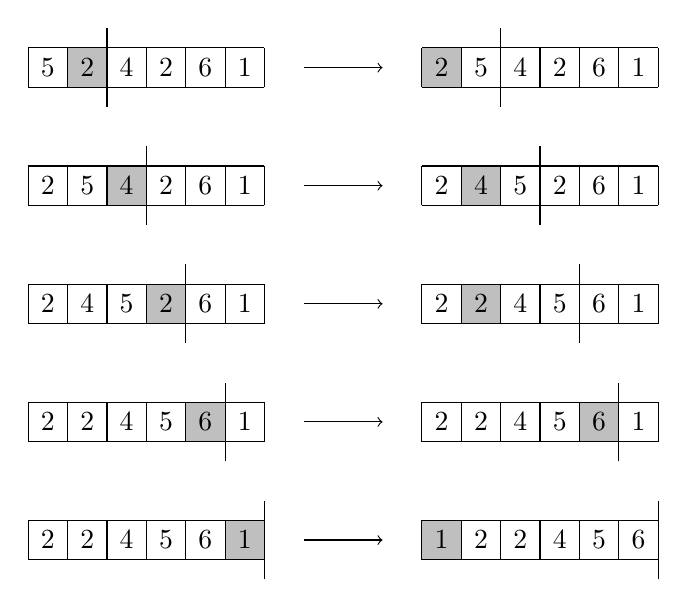
\begin{tikzpicture}[scale=0.5]
\begin{scope}
\fill[lightgray] (1,0) rectangle (2,1);
\draw (0,0) grid (6,1);
\foreach \x/\v in {0/5,1/2,2/4,3/2,4/6,5/1} \node at (0.5+\x,0.5) {\v};
\draw (2,-0.5) -- (2,1.5);
\draw[->] (7,0.5) -- (9,0.5);
\end{scope}
\begin{scope}[xshift=10cm]
\fill[lightgray] (0,0) rectangle (1,1);
\draw (0,0) grid (6,1);
\foreach \x/\v in {0/2,1/5,2/4,3/2,4/6,5/1} \node at (0.5+\x,0.5) {\v};
\draw (2,-0.5) -- (2,1.5);
\end{scope}
\begin{scope}[yshift=-3cm]
\fill[lightgray] (2,0) rectangle (3,1);
\draw (0,0) grid (6,1);
\foreach \x/\v in {0/2,1/5,2/4,3/2,4/6,5/1} \node at (0.5+\x,0.5) {\v};
\draw (3,-0.5) -- (3,1.5);
\draw[->] (7,0.5) -- (9,0.5);
\end{scope}
\begin{scope}[yshift=-3cm,xshift=10cm]
\fill[lightgray] (1,0) rectangle (2,1);
\draw (0,0) grid (6,1);
\foreach \x/\v in {0/2,1/4,2/5,3/2,4/6,5/1} \node at (0.5+\x,0.5) {\v};
\draw (3,-0.5) -- (3,1.5);
\end{scope}
\begin{scope}[yshift=-6cm]
\fill[lightgray] (3,0) rectangle (4,1);
\draw (0,0) grid (6,1);
\foreach \x/\v in {0/2,1/4,2/5,3/2,4/6,5/1} \node at (0.5+\x,0.5) {\v};
\draw (4,-0.5) -- (4,1.5);
\draw[->] (7,0.5) -- (9,0.5);
\end{scope}
\begin{scope}[yshift=-6cm,xshift=10cm]
\fill[lightgray] (1,0) rectangle (2,1);
\draw (0,0) grid (6,1);
\foreach \x/\v in {0/2,1/2,2/4,3/5,4/6,5/1} \node at (0.5+\x,0.5) {\v};
\draw (4,-0.5) -- (4,1.5);
\end{scope}
\begin{scope}[yshift=-9cm]
\fill[lightgray] (4,0) rectangle (5,1);
\draw (0,0) grid (6,1);
\foreach \x/\v in {0/2,1/2,2/4,3/5,4/6,5/1} \node at (0.5+\x,0.5) {\v};
\draw (5,-0.5) -- (5,1.5);
\draw[->] (7,0.5) -- (9,0.5);
\end{scope}
\begin{scope}[yshift=-9cm,xshift=10cm]
\fill[lightgray] (4,0) rectangle (5,1);
\draw (0,0) grid (6,1);
\foreach \x/\v in {0/2,1/2,2/4,3/5,4/6,5/1} \node at (0.5+\x,0.5) {\v};
\draw (5,-0.5) -- (5,1.5);
\end{scope}
\begin{scope}[yshift=-12cm]
\fill[lightgray] (5,0) rectangle (6,1);
\draw (0,0) grid (6,1);
\foreach \x/\v in {0/2,1/2,2/4,3/5,4/6,5/1} \node at (0.5+\x,0.5) {\v};
\draw (6,-0.5) -- (6,1.5);
\draw[->] (7,0.5) -- (9,0.5);
\end{scope}
\begin{scope}[yshift=-12cm,xshift=10cm]
\fill[lightgray] (0,0) rectangle (1,1);
\draw (0,0) grid (6,1);
\foreach \x/\v in {0/1,1/2,2/2,3/4,4/5,5/6} \node at (0.5+\x,0.5) {\v};
\draw (6,-0.5) -- (6,1.5);
\end{scope}
\end{tikzpicture}
\caption{Lisäysjärjestäminen taulukolle $[5,2,4,2,6,1]$.}
\label{fig:lisjar}
\end{figure}

Kuva \ref{fig:lisjar} näyttää esimerkin lisäysjärjestämisen
toiminnasta, kun järjes\-tettävänä on taulukko $[5,2,4,2,6,1]$.
Jokaisella rivillä algoritmi siirtää harmaataustaisen
alkion sen oikealle paikalle taulukon alkuosassa.
Pystyviiva ilmaisee kohdan, johon asti taulukko on järjestyksessä
siirron jälkeen.
Algoritmin päätteeksi tuloksena on järjestetty taulukko $[1,2,2,4,5,6]$.

Seuraava koodi toteuttaa lisäysjärjestämisen:

\begin{code}
for i = 1 to n-1
    j = i-1
    while j >= 0 and taulu[j] > taulu[j+1]
        swap(taulu[j],taulu[j+1])
        j -= 1
\end{code}

Koodi käy läpi taulukon kohdat $1 \dots n-1$
ja siirtää aina kohdassa $i$ olevan alkion
oikeaan paikkaan.
Tämä tapahtuu sisäsilmukalla,
jonka jokainen askel vaihtaa keskenään alkion
ja sen vasemmalla puolella olevan alkion
niin kauan, kuin vasen alkio on suurempi.
Huomaa pseudokoodin komento \texttt{swap}, joka ilmaisee,
että kaksi alkiota vaihdetaan keskenään.

Lisäysjärjestämisen tehokkuus riippuu siitä,
mikä on järjestettävän taulukon sisältö.
Algoritmi toimii sitä paremmin, mitä lähempänä järjestystä
taulukko on valmiiksi.
Jos taulukko on järjestyksessä,
aikaa kuluu vain $O(n)$, koska ei tarvitse siirtää
mitään alkioita.
Pahin tapaus algoritmille on kuitenkin, että taulukko on
\emph{käänteisessä} järjestyksessä,
jolloin jokainen alkio täytyy siirtää
taulukon alkuun ja aikaa kuluu $O(n^2)$.

\subsection{Inversiot}

\index{inversio}

Hyödyllinen käsite järjestämisalgoritmien analysoinnissa
on \emph{inversio}: kaksi taulukossa olevaa alkiota,
jotka ovat väärässä järjestyksessä.
Esimerkiksi taulukossa $[3,1,4,2]$ on kolme inversiota:
$(3,1)$, $(3,2)$ ja $(4,2)$.
Inversioiden määrä kertoo taulukon järjestyksestä:
mitä vähemmän inversioita taulukossa on,
sitä lähempänä se on järjestystä.
Erityisesti taulukko on järjestyksessä tarkalleen silloin,
kun siinä ei ole yhtään inversiota.

Kun järjestämisalgoritmi järjestää taulukon,
se \emph{poistaa} siitä inversioita.
Esimerkiksi aina kun
lisäysjärjestäminen vaihtaa vierekkäiset alkiot keskenään,
se poistaa taulukosta yhden inversion.
Niinpä lisäysjärjestämisen työmäärä on yhtä suuri
kuin järjestettävän taulukon inversioiden määrä.

Olemme jo todenneet, että pahin mahdollinen syöte
lisäysjärjestämiselle on käänteisessä järjestyksessä oleva taulukko.
Tällaisessa taulukossa jokainen alkiopari muodostaa inversion,
joten inversioiden määrä on
\[\frac{n(n-1)}{2}=O(n^2).\]
Entä kuinka hyvin lisäysjärjestäminen toimii \emph{keskimäärin}?
Jos oletamme, että taulukossa on $n$ eri alkiota satunnaisessa
järjestyksessä, jokainen taulukossa oleva alkiopari muodostaa
inversion todennäköisyydellä $1/2$.
Niinpä inversioiden määrän \emph{odotusarvo} on
\[\frac{n(n-1)}{4}=O(n^2),\]
eli aikaa kuluu neliöllinen määrä myös keskimääräisessä
tapauksessa.

Syy lisäysjärjestämisen hitauteen on,
että se ei poista taulukosta inversioita riittävän tehokkaasti.
Jos haluamme kehittää paremman järjestämis\-algoritmin,
se täytyy suunnitella niin, että se voi poistaa
useita inversioita \emph{yhtä aikaa}.
Käytännössä algoritmin täytyy pystyä siirtämään
väärässä paikassa oleva alkio tehokkaasti taulukon
toiselle puolelle.

\section{Järjestäminen ajassa $O(n \log n)$}

Seuraavaksi tutustumme kahteen tehokkaaseen
järjestämisalgoritmiin, jotka perustuvat rekursioon.
Molemmissa algoritmeissa on ideana
järjestää taulukko jakamalla se kahteen pienempään
osataulukkoon ja järjestämällä ne rekursiivisesti.
Tämän jälkeen järjestetyt osataulukot yhdistetään
kokonaiseksi järjestetyksi taulukoksi.

\subsection{Lomitusjärjestäminen}

\index{lomitusjärjestäminen}

\begin{figure}
\center
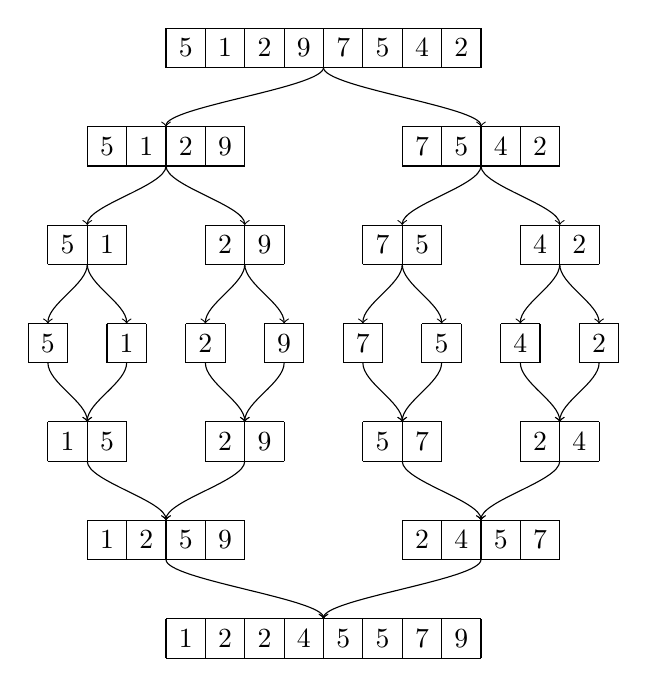
\begin{tikzpicture}[scale=0.5]
\begin{scope}
\draw (0,0) grid (8,1);
\foreach \x/\v in {0/5,1/1,2/2,3/9,4/7,5/5,6/4,7/2} \node at (0.5+\x,0.5) {\v};
\draw[->] (4,0) .. controls (4,-0.5) and (0,-1) .. (0,-1.5);
\draw[->] (4,0) .. controls (4,-0.5) and (8,-1) .. (8,-1.5);
\end{scope}
\begin{scope}[yshift=-2.5cm,xshift=-2cm]
\draw (0,0) grid (4,1);
\draw (8,0) grid (12,1);
\foreach \x/\v in {0/5,1/1,2/2,3/9,8/7,9/5,10/4,11/2} \node at (0.5+\x,0.5) {\v};
\draw[->] (2,0) .. controls (2,-0.5) and (0,-1) .. (0,-1.5);
\draw[->] (2,0) .. controls (2,-0.5) and (4,-1) .. (4,-1.5);
\draw[->] (10,0) .. controls (10,-0.5) and (8,-1) .. (8,-1.5);
\draw[->] (10,0) .. controls (10,-0.5) and (12,-1) .. (12,-1.5);
\end{scope}
\begin{scope}[yshift=-5cm,xshift=-3cm]
\draw (0,0) grid (2,1);
\draw (4,0) grid (6,1);
\draw (8,0) grid (10,1);
\draw (12,0) grid (14,1);
\foreach \x/\v in {0/5,1/1,4/2,5/9,8/7,9/5,12/4,13/2} \node at (0.5+\x,0.5) {\v};
\draw[->] (1,0) .. controls (1,-0.5) and (0,-1) .. (0,-1.5);
\draw[->] (1,0) .. controls (1,-0.5) and (2,-1) .. (2,-1.5);
\draw[->] (5,0) .. controls (5,-0.5) and (4,-1) .. (4,-1.5);
\draw[->] (5,0) .. controls (5,-0.5) and (6,-1) .. (6,-1.5);
\draw[->] (9,0) .. controls (9,-0.5) and (8,-1) .. (8,-1.5);
\draw[->] (9,0) .. controls (9,-0.5) and (10,-1) .. (10,-1.5);
\draw[->] (13,0) .. controls (13,-0.5) and (12,-1) .. (12,-1.5);
\draw[->] (13,0) .. controls (13,-0.5) and (14,-1) .. (14,-1.5);
\end{scope}
\begin{scope}[yshift=-7.5cm,xshift=-3.5cm]
\draw (0,0) grid (1,1);
\draw (2,0) grid (3,1);
\draw (4,0) grid (5,1);
\draw (6,0) grid (7,1);
\draw (8,0) grid (9,1);
\draw (10,0) grid (11,1);
\draw (12,0) grid (13,1);
\draw (14,0) grid (15,1);
\foreach \x/\v in {0/5,2/1,4/2,6/9,8/7,10/5,12/4,14/2} \node at (0.5+\x,0.5) {\v};
\draw[->] (0.5,0) .. controls (0.5,-0.5) and (1.5,-1) .. (1.5,-1.5);
\draw[->] (2.5,0) .. controls (2.5,-0.5) and (1.5,-1) .. (1.5,-1.5);
\draw[->] (4.5,0) .. controls (4.5,-0.5) and (5.5,-1) .. (5.5,-1.5);
\draw[->] (6.5,0) .. controls (6.5,-0.5) and (5.5,-1) .. (5.5,-1.5);
\draw[->] (8.5,0) .. controls (8.5,-0.5) and (9.5,-1) .. (9.5,-1.5);
\draw[->] (10.5,0) .. controls (10.5,-0.5) and (9.5,-1) .. (9.5,-1.5);
\draw[->] (12.5,0) .. controls (12.5,-0.5) and (13.5,-1) .. (13.5,-1.5);
\draw[->] (14.5,0) .. controls (14.5,-0.5) and (13.5,-1) .. (13.5,-1.5);
\end{scope}
\begin{scope}[yshift=-10cm,xshift=-3cm]
\draw (0,0) grid (2,1);
\draw (4,0) grid (6,1);
\draw (8,0) grid (10,1);
\draw (12,0) grid (14,1);
\foreach \x/\v in {0/1,1/5,4/2,5/9,8/5,9/7,12/2,13/4} \node at (0.5+\x,0.5) {\v};
\draw[->] (1,0) .. controls (1,-0.5) and (3,-1) .. (3,-1.5);
\draw[->] (5,0) .. controls (5,-0.5) and (3,-1) .. (3,-1.5);
\draw[->] (9,0) .. controls (9,-0.5) and (11,-1) .. (11,-1.5);
\draw[->] (13,0) .. controls (13,-0.5) and (11,-1) .. (11,-1.5);
\end{scope}
\begin{scope}[yshift=-12.5cm,xshift=-2cm]
\draw (0,0) grid (4,1);
\draw (8,0) grid (12,1);
\foreach \x/\v in {0/1,1/2,2/5,3/9,8/2,9/4,10/5,11/7} \node at (0.5+\x,0.5) {\v};
\draw[->] (2,0) .. controls (2,-0.5) and (6,-1) .. (6,-1.5);
\draw[->] (10,0) .. controls (10,-0.5) and (6,-1) .. (6,-1.5);
\end{scope}
\begin{scope}[yshift=-15cm]
\draw (0,0) grid (8,1);
\foreach \x/\v in {0/1,1/2,2/2,3/4,4/5,5/5,6/7,7/9} \node at (0.5+\x,0.5) {\v};
\end{scope}
\end{tikzpicture}
\caption{Lomitusjärjestäminen taulukolle $[5,1,2,9,7,5,4,2]$.}
\label{fig:lomjar}
\end{figure}

\emph{Lomitusjärjestäminen} (\emph{merge sort}) on rekursiivinen järjestämisalgoritmi,
joka perustuu taulukon puolituksiin.
Kun järjestettävänä on $n$-alkioinen taulukko,
se jaetaan keskeltä kahdeksi osataulukoksi,
joissa molemmissa on noin $n/2$ alkiota.
Tämän jälkeen osataulukot järjestetään erikseen rekursiivisesti
ja järjestetyt osataulukot \emph{lomitetaan} niin,
että niistä muodostuu kokonainen järjestetty taulukko.
Rekursio päättyy tapaukseen $n=1$, jolloin
taulukko on valmiiksi järjestyksessä eikä
tarvitse tehdä mitään.

Seuraava koodi esittää tarkemmin lomitusjärjestämisen toiminnan:

\begin{code}
procedure jarjesta(a,b)
    if a == b
        return
    k = (a+b)/2
    jarjesta(a,k)
    jarjesta(k+1,b)
    lomita(a,k,k+1,b)
\end{code}

Proseduuri \texttt{jarjesta} järjestää taulukon
välin $a \dots b$ (osataulukon kohdasta
$a$ kohtaan $b$), eli kun haluamme järjestää koko taulukon,
kutsumme proseduuria parametreilla $a=0$ ja $b=n-1$.
Proseduuri tarkastaa ensin, onko osataulukossa vain yksi alkio,
ja jos näin on, proseduuri päättyy heti.
Muuten se laskee muuttujaan $k$ järjestettävän välin keskikohdan
ja järjestää vasemman ja oikean puoliskon rekursiivisesti.
Lopuksi se kutsuu proseduuria \texttt{lomita},
joka yhdistää järjestetyt puoliskot.
Seuraava koodi näyttää, kuinka voimme toteuttaa tämän proseduurin:

\begin{code}
procedure lomita(a1, b1, a2, b2)
    a = a1, b = b2
    for i = a to b
        if a2 > b2 or (a1 <= b1 and taulu[a1] <= taulu[a2])
            apu[i] = taulu[a1]
            a1 += 1
        else
            apu[i] = taulu[a2]
            a2 += 1
    for i = a to b
        taulu[i] = apu[i]
\end{code}

Parametreina annetaan välit $a_1 \dots b_1$ ja $a_2 \dots b_2$,
missä $b_1+1=a_2$.
Proseduuri olettaa, että näillä väleillä olevat 
taulukon alkiot on järjestetty,
ja se lomittaa alkiot niin, että
taulukon koko väli $a_1 \dots b_2$ on järjestetty.
Proseduurin perustana on silmukka, joka käy läpi välejä
$a_1 \dots b_1$ ja $a_2 \dots b_2$ rinnakkain ja valitsee
aina seuraavaksi pienimmän alkion lopulliseen järjestykseen.
Jotta lomitus ei sotke taulukkoa,
proseduuri käyttää globaalia aputaulukkoa,
johon se ensin muodostaa järjestetyn osataulukon,
ja kopioi sitten alkiot aputaulukosta varsinaiseen taulukkoon.

Kuva \ref{fig:lomjar} näyttää, miten lomitusjärjestäminen
toimii, kun sille annetaan taulukko $[5,1,2,9,7,5,4,2]$.
Algoritmi puolittaa ensin taulukon kahdeksi osataulukoksi
$[5,1,2,9]$ ja $[7,5,4,2]$ ja järjestää molemmat
osataulukot kutsumalla itseään.
Kun algoritmi saa sitten järjestettäväksi taulukon $[5,1,2,9]$,
se jakaa taulukon edelleen osataulukoiksi $[5,1]$ ja $[2,9]$, jne.
Lopulta jäljellä on vain yhden alkion kokoisia
osataulukoita, jotka ovat valmiiksi järjestyksessä.
Tällöin rekursiivinen jakautuminen päättyy ja algoritmi
alkaa koota järjestettyjä osataulukkoja pienimmästä suurimpaan.

Kuinka tehokas lomitusjärjestäminen on?
Koska jokainen proseduurin \texttt{jarjesta} kutsu
puolittaa taulukon koon, rekursiosta muodostuu
$O(\log n)$ tasoa  (kuva \ref{fig:lomjar}).
Ylimmällä tasolla on taulukko,
jossa on $n$ alkiota,
seuraavalla tasolla on kaksi taulukkoa,
joissa on $n/2$ alkiota,
seuraavalla tasolla on neljä taulukkoa,
joissa on $n/4$ alkiota, jne.
Proseduuri \texttt{lomita} toimii lineaarisessa ajassa,
joten kullakin tasolla taulukoiden lomittamiset vievät yhteensä
aikaa $O(n)$.
Niinpä algoritmin kokonaisaikavaativuus on $O(n \log n)$.

\subsection{Pikajärjestäminen}

\index{pikajärjestäminen}

\emph{Pikajärjestäminen} (\emph{quick sort}) tarjoaa toisenlaisen rekursiivisen
lähestymis\-tavan taulukon järjestämiseen.
Kun saamme järjestettäväksi taulukon, valitsemme ensin jonkin
sen alkioista \emph{jakoalkioksi} (\emph{pivot}).
Tämän jälkeen siirräm\-me alkioita niin,
että jakoalkiota pienemmät alkiot ovat sen vasemmalla puolella,
suuremmat alkiot ovat sen oikealla puolella ja
yhtä suuret alkiot voivat olla kummalla tahansa puolella.
Lopuksi järjestämme rekursiivisesti osataulukot,
jotka muodostuvat jakoalkion vasemmalle ja oikealle puolelle.

Seuraava koodi esittää pikajärjestämisen toiminnan:

\begin{code}
procedure jarjesta(a, b)
    if a >= b
        return
    k = jako(a,b)
    jarjesta(a,k-1)
    jarjesta(k+1,b)
\end{code}

Proseduuri \texttt{jarjesta} järjestää taulukon välillä
$a \dots b$ olevat alkiot.
Jos väli on tyhjä tai siinä on vain yksi alkio,
proseduuri ei tee mitään.
Muuten se kutsuu funktiota \texttt{jako}, joka valitsee jakoalkion,
siirtää taulukon alkioita sen mukaisesti
ja palauttaa sitten kohdan $k$,
jossa jakoalkio on siirtojen jälkeen.
Tämän jälkeen taulukon vasen osa (väli $a \dots k-1$)
ja oikea osa (väli $k+1 \dots b$) järjestetään rekursiivisesti.

Funktion \texttt{jako} voi toteuttaa monella tavalla,
koska voimme valita minkä tahansa alkion jakoalkioksi ja
lisäksi on monia tapoja siirtää alkioita.
Käy\-tämme tässä esimerkkinä seuraavaa toteutusta:

\begin{code}
function jako(a,b):
    k = a
    for i = a+1 to b
        if taulu[i] < taulu[a]
            k += 1
            swap(taulu[i],taulu[k])
    swap(taulu[a],taulu[k])
    return k
\end{code}

Tässä jakoalkio on aina kohdassa $a$ oleva välin ensimmäinen alkio.
Funktio käy läpi välin alkiot ja siirtää
jakoalkiota pienempiä alkioita taulukon alkuosaan.
Muuttuja $k$ määrittää kohdan,
johon seuraava pienempi alkio siirretään.
Lopuksi jakoalkio itse siirretään keskelle
kohtaan $k$, jonka funktio myös palauttaa.

\begin{figure}
\center
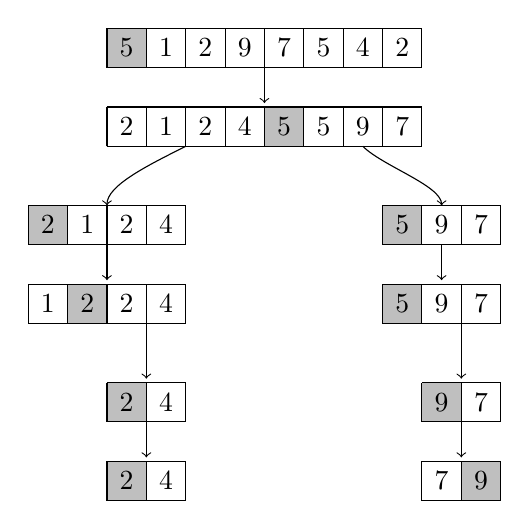
\begin{tikzpicture}[scale=0.5]
\begin{scope}
\fill[lightgray] (0,0) rectangle (1,1);
\draw (0,0) grid (8,1);
\foreach \x/\v in {0/5,1/1,2/2,3/9,4/7,5/5,6/4,7/2} \node at (0.5+\x,0.5) {\v};
\fill[lightgray] (4,-2) rectangle (5,-1);
\draw (0,-2) grid (8,-1);
\foreach \x/\v in {0/2,1/1,2/2,3/4,4/5,5/5,6/9,7/7} \node at (0.5+\x,-1.5) {\v};
\draw[->] (4,0) -- (4,-0.9);
\draw[->] (2,-2) .. controls (1,-2.5) and (0,-3) .. (0,-3.5);
\draw[->] (6.5,-2) .. controls (7,-2.5) and (8.5,-3) .. (8.5,-3.5);
\end{scope}
\begin{scope}[yshift=-4.5cm,xshift=-2cm]
\fill[lightgray] (0,0) rectangle (1,1);
\draw (0,0) grid (4,1);
\fill[lightgray] (9,0) rectangle (10,1);
\draw (9,0) grid (12,1);
\fill[lightgray] (1,-2) rectangle (2,-1);
\draw (0,-2) grid (4,-1);
\fill[lightgray] (9,-2) rectangle (10,-1);
\draw (9,-2) grid (12,-1);
\foreach \x/\v in {0/2,1/1,2/2,3/4,9/5,10/9,11/7} \node at (0.5+\x,0.5) {\v};
\foreach \x/\v in {0/1,1/2,2/2,3/4,9/5,10/9,11/7} \node at (0.5+\x,-1.5) {\v};
\draw[->] (2,0) -- (2,-0.9);
\draw[->] (10.5,0) -- (10.5,-0.9);
\draw[->] (3,-2) -- (3,-3.4);
\draw[->] (11,-2) -- (11,-3.4);
\end{scope}
\begin{scope}[yshift=-9cm,xshift=-2cm]
\fill[lightgray] (2,0) rectangle (3,1);
\draw (2,0) grid (4,1);
\fill[lightgray] (10,0) rectangle (11,1);
\draw (10,0) grid (12,1);
\fill[lightgray] (2,-2) rectangle (3,-1);
\draw (2,-2) grid (4,-1);
\fill[lightgray] (11,-2) rectangle (12,-1);
\draw (10,-2) grid (12,-1);
\foreach \x/\v in {2/2,3/4,10/9,11/7} \node at (0.5+\x,0.5) {\v};
\foreach \x/\v in {2/2,3/4,10/7,11/9} \node at (0.5+\x,-1.5) {\v};
\draw[->] (3,0) -- (3,-0.9);
\draw[->] (11,0) -- (11,-0.9);
\end{scope}
\end{tikzpicture}
\caption{Pikajärjestäminen taulukolle $[5,1,2,9,7,5,4,2]$.}
\label{fig:pikjar}
\end{figure}

Kuva \ref{fig:pikjar} näyttää, miten pikajärjestäminen toimii, kun sille
annetaan taulukko $[5,1,2,9,7,5,4,2]$.
Jokaisessa vaiheessa harmaa tausta osoittaa jakoalkion sijainnin.
Aluksi koko taulukon jakoalkio on 5 ja algoritmi siirtää
alkioita niin, että jakoalkion vasemmalla puolella
ovat alkiot $[2,1,2,4]$ ja oikealla puolella alkiot $[5,9,7]$.
Tämän jälkeen vasen ja oikea osataulukko järjestetään
vastaavasti rekursiivisesti.

Pikajärjestämisen tehokkuuteen vaikuttaa, miten alkiot jakautuvat
jakoalkion eri puolille.
Jos hyvin käy, jakoalkion kummallekin puolelle
siirretään suunnilleen yhtä monta alkiota.
Tällöin taulukon koko puolittuu jokaisen jaon jälkeen
ja pikajärjestäminen toimii tehokkaasti.
Koska funktio \texttt{jako} toimii lineaarisessa ajassa,
pikajärjestäminen vie tässä tapauksessa aikaa
$O(n \log n)$ samaan tapaan kuin lomitusjärjestäminen.
Uhkana on kuitenkin, että jakoalkio jakaa taulukon osiin \emph{epätasaisesti}.
Kuva \ref{fig:pikpah} näyttää tilanteen, jossa jokaisessa jaossa
kaikki alkiot jäävät jakoalkion oikealle puolelle.
Tällöin pikajärjestäminen viekin aikaa $O(n^2)$, koska rekursiivisia
tasoja on $O(n)$.
Selvästikään \emph{ei} ole kaikissa tilanteissa hyvä tapa
valita taulukon ensimmäinen alkio jakoalkioksi.
Esimerkiksi valmiiksi järjestyksessä olevan
taulukon järjestäminen vie silloin aikaa $O(n^2)$.

\begin{figure}
\center
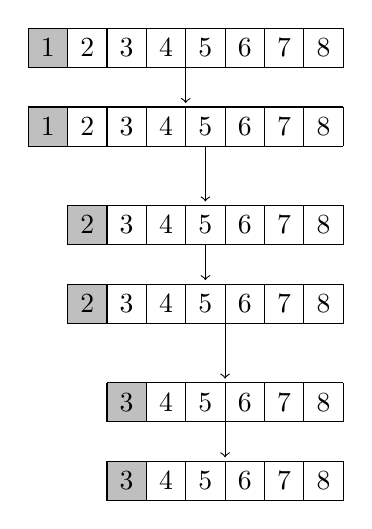
\begin{tikzpicture}[scale=0.5]
\begin{scope}
\fill[color=lightgray] (0,0) rectangle (1,1);
\draw (0,0) grid (8,1);
\foreach \x/\v in {0/1,1/2,2/3,3/4,4/5,5/6,6/7,7/8} \node at (0.5+\x,0.5) {\v};
\fill[color=lightgray] (0,-2) rectangle (1,-1);
\draw (0,-2) grid (8,-1);
\foreach \x/\v in {0/1,1/2,2/3,3/4,4/5,5/6,6/7,7/8} \node at (0.5+\x,-1.5) {\v};
\draw[->] (4,-0) -- (4,-0.9);
\draw[->] (4.5,-2) -- (4.5,-3.4);
\end{scope}
\begin{scope}[xshift=1cm,yshift=-4.5cm]
\fill[color=lightgray] (0,0) rectangle (1,1);
\draw (0,0) grid (7,1);
\foreach \x/\v in {0/2,1/3,2/4,3/5,4/6,5/7,6/8} \node at (0.5+\x,0.5) {\v};
\fill[color=lightgray] (0,-2) rectangle (1,-1);
\draw (0,-2) grid (7,-1);
\foreach \x/\v in {0/2,1/3,2/4,3/5,4/6,5/7,6/8} \node at (0.5+\x,-1.5) {\v};
\draw[->] (3.5,-0) -- (3.5,-0.9);
\draw[->] (4,-2) -- (4,-3.4);
\end{scope}
\begin{scope}[xshift=2cm,yshift=-9cm]
\fill[color=lightgray] (0,0) rectangle (1,1);
\draw (0,0) grid (6,1);
\foreach \x/\v in {0/3,1/4,2/5,3/6,4/7,5/8} \node at (0.5+\x,0.5) {\v};
\fill[color=lightgray] (0,-2) rectangle (1,-1);
\draw (0,-2) grid (6,-1);
\foreach \x/\v in {0/3,1/4,2/5,3/6,4/7,5/8} \node at (0.5+\x,-1.5) {\v};
\draw[->] (3,-0) -- (3,-0.9);
\end{scope}
\end{tikzpicture}
\caption{Pikajärjestämisen pahin tapaus: jokaisessa jaossa kaikki
alkiot jäävät jakoalkion toiselle puolelle.}
\label{fig:pikpah}
\end{figure}

Oma lukunsa on tilanne, jossa taulukossa on paljon samoja alkioita.
Ääritapauksena \emph{jokainen} alkio on sama,
mikä on käytännössä hyvin mahdollinen syöte.
Tällöin tässä esitetty funktio \texttt{jako} tuottaa aina huonon jaon,
jossa kaikki alkiot menevät jakoalkion oikealle puolelle.
Ei siis riitä, että jakoalkio on valittu hyvin,
vaan myös tapa, jolla alkioita siirretään taulukossa,
vaikuttaa algoritmin tehokkuuteen.

Miten meidän tulisi sitten toteuttaa pikajärjestäminen?
Algoritmista on kehitetty vuosien aikana suuri määrä muunnelmia,
jotka pyrkivät parantamaan sen toimintaa eri tilanteissa.
Yksi kehittyneempi tapa valita jakoalkio on ottaa tarkasteluun
taulukon ensimmäinen, keskimmäinen ja viimeinen alkio ja valita
jakoalkioksi järjestyksessä keskimmäinen näistä kolmesta alkiosta.
Tällainen valinta toimii käytännössä hyvin monissa tilanteissa.
Parempi tapa toteuttaa alkioiden siirtäminen on puolestaan
käydä läpi rinnakkain alkioita alusta ja lopusta ja
pitää huoli siitä, että jakokohta jää keskelle, jos kaikki alkiot
ovat yhtä suuria.
Pikajärjestämisen toteuttaminen hyvin ei ole helppo tehtävä,
vaan vaatii paljon huolellisuutta.

\subsection{Algoritmien vertailua}

\begin{table}
\center
\begin{tabular}{llll}
algoritmi & tehokkuus & lisätila & vakaa \\
\hline
lisäysjärjestäminen & $O(n^2)$ & $O(1)$ & kyllä \\
lomitusjärjestäminen & $O(n \log n)$ & $O(n)$ & kyllä \\
pikajärjestäminen (hyvä tapaus) & $O(n \log n)$ & $O(\log n)$ & ei \\
pikajärjestäminen (huono tapaus) & $O(n^2)$ & $O(n)$ & ei \\
\end{tabular}
\caption{Järjestämisalgoritmien vertailua.}
\label{tab:jaralg}
\end{table}

\index{vakaus}

Taulukossa \ref{tab:jaralg} on yhteenveto tähän mennessä
käsitellyistä järjestämis\-algoritmeista.
Algoritmin lisätila tarkoittaa sen tilavaativuutta,
eli paljonko tilaa algoritmi tarvitsee järjestettävän taulukon lisäksi.
Lisäysjärjestäminen käyttää vain yksittäisiä muuttujia,
joten sen lisätila on $O(1)$.
Lomitusjärjes\-tämisessä lomittaminen käyttää aputaulukkoa,
mistä aiheutuu lisätila $O(n)$.
Pikajärjestämisessä puolestaan rekursiivinen kutsupino
vie tilaa muistissa riippuen rekursion syvyydestä.
Algoritmi on \emph{vakaa} (\emph{stable}), jos se säilyttää yhtä suuret alkiot
alkuperäisessä järjestyksessä.
Lisäysjärjestäminen ja lomitusjärjes\-täminen ovat vakaita,
koska ne eivät vaihda koskaan yhtä suurten alkioiden järjestystä,
mutta pikajärjestäminen saattaa tehdä näin jakoalkion valinnan jälkeen.
Algoritmin vakaudesta voi olla hyötyä sovelluksissa.

Meillä on nyt siis kaksi rekursiivista järjestämisalgoritmia:
lomitusjärjestä\-minen toimii \emph{aina} ajassa $O(n \log n)$,
kun taas pikajärjestäminen toimii \emph{ehkä} ajassa $O(n \log n)$,
mutta saattaa viedä aikaa $O(n^2)$.
Vaatii monenlaista virittelyä,
ennen kuin pikajärjestämisen saa toimimaan tehokkaasti
edes tapauksissa, joissa taulukko on valmiiksi järjestyksessä
tai kaikki alkiot ovat samoja.
Miksi haluaisimme koskaan käyttää epävarmaa pikajärjestämistä,
kun voimme käyttää myös varmasti tehokasta lomitusjärjestämistä?

\index{vakiokerroin}

Syynä on, että pikajärjestämisen \emph{vakiokertoimet} ovat pienet.
Kokemus on osoittanut, että kun toteutamme lomitusjärjestämisen ja
pikajärjestämisen ja mittaamme algoritmien todellisia suoritusaikoja,
pikajärjestäminen toimii usein nopeammin.
Näin tapahtuu siitä huolimatta, että pikajärjestämisen pahimman
tapauksen aikavaativuus on $O(n^2)$.
Käytännössä pahin tapaus on kuitenkin harvinainen,
jos jakoalkion valinta ja alkioiden siirtäminen on toteutettu huolellisesti.

\index{hybridialgoritmi}

Jos taulukko on pieni, $O(n^2)$-aikainen lisäysjärjestäminen
toimii käytän\-nössä nopeammin kuin rekursiiviset algoritmit,
koska sen vakiokertoimet ovat hyvin pienet.
Yksi mahdollisuus onkin toteuttaa \emph{hybridialgoritmi} (\emph{hybrid algorithm}),
jossa suuret taulukot järjes\-tetään rekursiivisesti
ja pienet taulukot järjes\-tetään lisäysjärjestämisellä.
Tällöin eri algoritmien hyvät puolet pääsevät osaksi
kokonaisalgoritmia.
Käytännössä hybridialgoritmin voi tehdä niin,
että valitaan jokin sopiva raja $k$ ja
taulukko järjestetään rekursiivisesti,
jos siinä on ainakin $k$ alkiota, ja muuten lisäysjärjestämisellä.

\section{Järjestämisen alaraja}

Olisiko mahdollista luoda järjestämisalgoritmi, joka toimisi
nopeammin kuin $O(n \log n)$?
Osoittautuu, että tämä \emph{ei} ole mahdollista,
jos oletamme, että algoritmin tulee perustua taulukon
alkioiden vertailuihin.
Vertailuihin perustuva järjestämisalgoritmi järjestää taulukon
tekemällä joukon vertailuja muotoa
''onko alkio $x$ suurempi kuin alkio $y$?''.

Vertailuihin perustuva järjestämisalgoritmi on \emph{yleiskäyttöinen}:
se pystyy järjestämään mitä tahansa alkioita,
kunhan meillä on keino saada selville kahden alkion suuruusjärjestys.
Tämä on ominaisuus, jota yleensä ottaen toivomme
järjestämisalgoritmilta, joten vertailuihin perustuminen
on luonteva rajoitus.
Kaikki tähän mennessä käsittelemämme järjestämisalgoritmit
ovat olleet vertailuihin perustuvia.

\subsection{Alarajatodistus}

Voimme ajatella vertailuihin perustuvaa järjestämistä
\emph{prosessina}, jossa jokainen vertailu antaa tietoa
taulukosta ja auttaa viemään taulukkoa lähemmäs järjestystä.
Oletamme, että taulukon alkiot ovat
$1,2,\dots,n$, jolloin on $n!$ vaihtoehtoa, mikä
on taulukon alkuperäinen järjestys.
Jotta järjestämisalgoritmi voisi toimia oikein,
sen täytyy käsitellä jokainen järjestys eri tavalla.

Esimerkiksi jos $n=3$, taulukon mahdolliset järjestykset alussa ovat
$[1,2,3]$, $[1,3,2]$, $[2,1,3]$, $[2,3,1]$, $[3,1,2]$ ja $[3,2,1]$.
Algoritmi voi vertailla ensin vaikkapa ensimmäistä ja toista alkiota.
Jos ensimmäinen alkio on pienempi, voimme päätellä,
että mahdolliset taulukot ovat $[1,2,3]$, $[1,3,2]$ ja $[2,3,1]$.
Jos taas ensimmäinen alkio on suurempi,
mahdolliset taulukot ovat $[2,1,3]$, $[3,1,2]$ ja $[3,2,1]$.
Tämän jälkeen voimme jatkaa vertailuja samaan tapaan
ja saada lisää tietoa taulukosta.
Algoritmi voi päättyä vasta silloin, kun jäljellä on vain yksi
mahdollinen taulukko, jotta voimme olla varmoja, että olemme
järjestäneet taulukon oikein.

Tärkeä seikka on, että jokaisessa vertailussa ainakin puolet jäljellä
olevista taulukoista voi täsmätä vertailun tulokseen.
Niinpä jos algoritmilla käy huono tuuri, se voi enintään puolittaa
taulukoiden määrän joka askeleella.
Tämä tarkoittaa, että algoritmi joutuu tekemään pahimmassa
tapauksessa ainakin $\log(n!)$ vertailua.
Logaritmien laskusääntöjen perusteella
\[
\log(n!) = \log(1)+\log(2)+\dots+\log(n).
\]
Saamme tälle summalle alarajan ottamalla huomioon vain
$n/2$ viimeistä termiä ja arvioimalla niitä alaspäin niin, 
että jokaisen termin suuruus on vain $\log(n/2)$. Tuloksena on alaraja
\[
\log(n!) \ge (n/2) \log(n/2),
\]
mikä tarkoittaa, että algoritmi joutuu tekemään
pahimmassa tapauksessa $\Omega(n \log n)$ vertailua.

\subsection{Laskemisjärjestäminen}

\index{laskemisjärjestäminen}

Millainen olisi sitten järjestämisalgoritmi,
joka ei perustu vertailuihin ja toimii
tehokkaammin kuin $O(n \log n)$?
\emph{Laskemisjärjestäminen} (\emph{counting sort})
on $O(n)$-aikainen järjestämisalgoritmi,
jonka toiminta perustuu oletukseen, että taulukon alkiot
ovat sopivan pieniä kokonaislukuja.
Algoritmi olettaa, että jokainen alkio on
kokonaisluku välillä $0 \dots k$, missä $k=O(n)$.

Algoritmi luo \emph{kirjanpidon}, joka kertoo,
montako kertaa mikä\-kin mahdollinen luku välillä $0 \dots k$
esiintyy taulukossa.
Seuraavassa koodissa kirjanpito tallennetaan
taulukkoon \texttt{laskuri} niin, että
$\texttt{laskuri}[x]$ ilmaisee,
montako kertaa luku $x$ esiintyy taulukossa.
Tämän kirjanpidon avulla voimme luoda suoraan
lopullisen järjestetyn taulukon.

\begin{code}
for i = 0 to n-1
    laskuri[taulu[i]] += 1
i = 0
for x = 0 to k
    for j = 1 to laskuri[x]
        taulu[i] = x
        i += 1
\end{code}

Algoritmin molemmat vaiheet vievät aikaa $O(n)$,
joten se toimii ajassa $O(n)$ ja on käytännössä hyvin tehokas.
Algoritmi ei ole kuitenkaan yleinen järjestämisalgoritmi,
koska sitä voi käyttää vain silloin,
kun taulukon kaikki alkiot ovat sopivan pieniä kokonaislukuja.

\section{Ohjelmointikielten toteutukset}

Vaikka on hyödyllistä tuntea järjestämisen teoriaa,
käytännössä ei ole hyvä idea toteuttaa itse
järjestämisalgoritmia, koska nykypäivän ohjelmointikielissä
on valmiit työkalut järjestämiseen.
Valmiin algoritmin käyttämisessä on etuna,
että se on varmasti hyvin toteutettu ja tehokas.
Lisäksi ohjelmoijan aikaa säästyy,
kun algoritmia ei joudu toteuttamaan itse.

\subsection{Java}

Javan standardikirjaston metodi \texttt{Arrays.sort}
järjestää sille annetun taulukon seuraavaan tapaan:

\begin{code}
int[] taulu = {4,2,5,8,2,1,5,6};
Arrays.sort(taulu);
// tulos: [1,2,2,4,5,5,6,8]
\end{code}

Metodin sisäinen toiminta riippuu siitä,
minkä \emph{tyyppistä} tietoa taulukossa on.
Jos taulukon alkiot ovat alkeistyyppisiä
(esimerkiksi \texttt{int}), Java käyttää 
pikajärjestämisen muunnelmaa,
jossa on kaksi jakoalkiota.
Jos taas alkiot ovat oliotyyppisiä
(esimerkiksi \texttt{String}),
algoritmina on Timsort, joka on optimoitu lomitusjärjestäminen.

Kun \texttt{Arrays.sort} järjestää olioita sisältävän taulukon,
se kutsuu metodia \texttt{compareTo} aina, kun se haluaa selvittää
kahden alkion suuruusjärjestyksen.
Metodin tulee palauttaa negatiivinen arvo, nolla tai positiivinen arvo
sen mukaan, onko olio itse pienempi, yhtä suuri vai suurempi
kuin parametrina annettu olio.
Javan omissa luokissa tällainen metodi on olemassa valmiina.
Esimerkiksi \texttt{"apina".compareTo("banaani")} palauttaa
negatiivisen arvon, koska apina on ennen banaania aakkosjärjestyksessä.

Tämän ansiosta voimme järjestää suoraan taulukoita,
joissa on esimerkiksi merkkijonoja.
Jos haluamme, että Java pystyy järjestämään omien luokkien olioita,
meidän täytyy toteuttaa itse luokkaan metodi \texttt{compareTo} ja
merkitä, että luokka toteuttaa rajapinnan \texttt{Comparable}.

Esimerkiksi seuraava koodi toteuttaa luokan \texttt{Piste},
johon voidaan tallentaa pisteen x- ja y-koordinaatit.
Luokassa on metodi \texttt{compareTo}, joka määrittelee,
että pisteet järjestetään ensisijaisesti x-koordinaatin ja
toissijaisesti y-koordinaatin mukaan.

\begin{code}
public class Piste implements Comparable<Piste> {
    private int x, y;
    
    public Piste(int x, int y) {
        this.x = x;
        this.y = y;
    }

    public int compareTo(Piste p) {
        if (this.x != p.x) {
            return this.x - p.x;
        } else {
            return this.y - p.y;
        }
    }
}
\end{code}

Tässä metodi \texttt{compareTo} palauttaa
x-koordinaattien erotuksen, jos x-koordinaatit eivät ole samat,
ja muuten y-koordinaattien erotuksen.
Metodi olettaa, että koordinaattien erotus voidaan esittää
\texttt{int}-tyyppisenä arvona.

Voimme nyt järjestää taulukollisen pisteitä näin:

\begin{code}
Piste[] pisteet = {new Piste(1,3),
                     new Piste(2,3),
                     new Piste(1,2)};
Arrays.sort(pisteet);
// tulos: [(1,2),(1,3),(2,3)]
\end{code}

\subsection{Python}

Pythonissa metodi \texttt{sort} järjestää listan sisällön:

\begin{code}
lista = [4,2,5,8,2,1,5,6]
lista.sort()
# tulos: [1,2,2,4,5,5,6,8]
\end{code}

Toinen tapa on käyttää funktiota \texttt{sorted},
joka palauttaa järjestetyn kopion parametrina annetusta listasta:

\begin{code}
kopio = sorted(lista)
\end{code}

Python käyttää järjestämiseen Timsort-algoritmia,
joka on optimoitu lomitusjärjestäminen.
Sama algoritmi on käytössä Javassa silloin,
kun taulukossa on olioita, ja algoritmi on kulkeutunut
Javaan Pythonista.

Järjestäminen toimii automaattisesti myös silloin,
kun listan alkiot muodostuvat useammasta osasta:

\begin{code}
lista = [(1,3),(2,3),(1,2)]
lista.sort()
# tulos: [(1,2),(1,3),(2,3)]
\end{code}

Oletuksena alkiot järjestetään pienimmästä suurimpaan,
mutta voimme muuttaa suunnan parametrilla \texttt{reverse}:

\begin{code}
lista.sort(reverse=True)
\end{code}

Lisäksi voimme antaa parametrilla \texttt{key} funktion,
joka muuntaa alkion avaimeksi, jonka mukaan järjestäminen tapahtuu.
Esimerkiksi seuraava koodi järjestää luvut niiden \emph{itseisarvon} mukaan:

\begin{code}
lista = [4,-2,-7,5,1]
lista.sort(key=abs)
# tulos: [1,-2,4,5,-7]
\end{code}

\section{Järjestämisen sovelluksia}

Järjestämisen merkitys algoritmiikassa on,
että voimme ratkaista monia ongelmia tehokkaasti, 
kunhan aineisto on järjestyksessä.
Niinpä yleinen tapa luoda tehokas algoritmi on järjestää
ensin syöte ajassa $O(n \log n)$ ja hyödyntää sitten
tavalla tai toisella järjestystä algoritmin loppuosassa.

\subsection{Taulukkoalgoritmeja}

\label{sec:taukas}

Järjestämisen avulla voimme ratkaista ajassa
$O(n \log n)$ monia taulukoihin liittyviä tehtäviä.
Käymme seuraavaksi läpi kaksi tällaista tehtävää.

Ensimmäinen tehtävämme on laskea,
montako \emph{eri} alkiota annetussa taulukossa on.
Esimerkiksi taulukko $[2,1,4,2,4,2]$ sisältää kolme
eri alkiota: $1$, $2$ ja $4$.
Voimme ratkaista tehtävän järjestämällä ensin taulukon,
minkä jälkeen yhtä suuret alkiot ovat vierekkäin.
Tämän jälkeen saamme laskettua vastauksen helposti,
koska riittää tutkia, monessako taulukon kohdassa on
\emph{vierekkäin} kaksi eri alkiota.
Voimme toteuttaa algoritmin näin:

\begin{code}
sort(taulu)
laskuri = 1
for i = 1 to n-1
    if taulu[i-1] != taulu[i]
        laskuri += 1
print(laskuri)
\end{code}

Algoritmi järjestää ensin taulukon ajassa $O(n \log n)$,
minkä jälkeen se käy läpi taulukon sisällön for-silmukalla
ajassa $O(n)$.
Tämän ansiosta algoritmi vie aikaa yhteensä $O(n \log n)$.


Entä jos haluammekin selvittää, mikä on taulukon \emph{yleisin} alkio?
Esimerkiksi taulukon $[2,1,4,2,4,2]$ yleisin alkio on $2$,
joka esiintyy kolme kertaa taulukossa.
Tämäkin tehtävä ratkeaa järjestämisen avulla, koska
järjestämisen jälkeen yhtä suuret alkiot ovat peräkkäin ja
meidän riittää etsiä pisin samaa alkiota toistava osuus.
Voimme toteuttaa algoritmin seuraavasti:

\begin{code}
sort(taulu)
maara = 1
suurin = 1
yleisin = taulu[0]
for i = 1 to n-1
    if taulu[i-1] != taulu[i]
        maara = 0
    maara += 1
    if maara > suurin
        suurin = maara
        yleisin = taulu[i]
print(yleisin)
\end{code}

Tässäkin algoritmissa järjestäminen vie aikaa $O(n \log n)$ ja
for-silmukka vie aikaa $O(n)$, joten algoritmin
kokonaisaikavaativuus on $O(n \log n)$.

\subsection{Binäärihaku}

\index{binäärihaku}

\emph{Binäärihaku} (\emph{binary search}) on menetelmä, jonka avulla voimme löytää alkion
järjestetystä taulukosta ajassa $O(\log n)$.
Ideana on pitää yllä hakuväliä, jossa etsittävä alkio voi olla,
ja puolittaa väli joka askeleella tutkimalla välin
keskimmäisenä olevaa alkiota.
Koska taulukko on järjestyksessä, voimme aina päätellä,
kumpaan suuntaan hakua tulee jatkaa.

Seuraava koodi etsii binäärihaulla taulukosta alkiota $x$:

\begin{code}
a = 0
b = n-1
while a <= b
    k = (a+b)/2
    if taulu[k] == x
        // alkio löytyi
        break
    if taulu[k] < x
        a = k+1
    if taulu[k] > x
        b = k-1
\end{code}

Algoritmi pitää yllä hakuväliä $[a,b]$, joka on aluksi $[0,n-1]$,
koska alkio $x$ saattaa olla missä tahansa kohdassa taulukossa.
Joka askeleella algoritmi tarkastaa välin keskellä kohdassa
$k=\lfloor (a+b)/2 \rfloor$ olevan alkion.
Jos kyseinen alkio on $x$, haku päättyy.
Jos taas alkio on pienempi kuin $x$, haku jatkuu välin
oikeaan puoliskoon,
ja jos alkio on suurempi kuin $x$, haku jatkuu välin
vasempaan puoliskoon.
Koska välin koko puolittuu joka askeleella,
binäärihaun aikavaativuus on $O(\log n)$.

\begin{figure}
\center
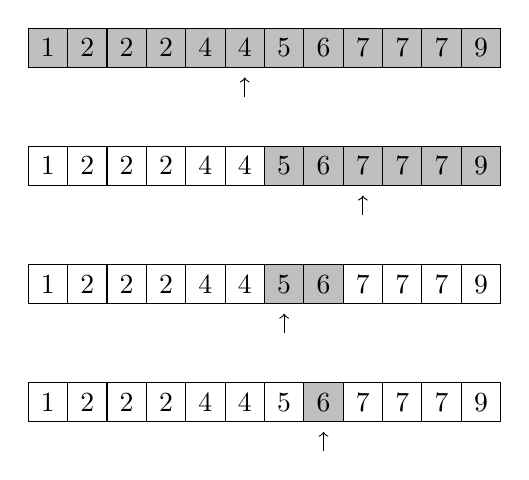
\begin{tikzpicture}[scale=0.5]
\begin{scope}
\fill[color=lightgray] (0,0) rectangle (12,1);
\draw (0,0) grid (12,1);
\foreach \x/\v in {0/1,1/2,2/2,3/2,4/4,5/4,6/5,7/6,8/7,9/7,10/7,11/9} \node at (0.5+\x,0.5) {\v};
\draw[->] (5.5,-0.75) -- (5.5,-0.25);
\end{scope}
\begin{scope}[yshift=-3cm]
\fill[color=lightgray] (6,0) rectangle (12,1);
\draw (0,0) grid (12,1);
\foreach \x/\v in {0/1,1/2,2/2,3/2,4/4,5/4,6/5,7/6,8/7,9/7,10/7,11/9} \node at (0.5+\x,0.5) {\v};
\draw[->] (8.5,-0.75) -- (8.5,-0.25);
\end{scope}
\begin{scope}[yshift=-6cm]
\fill[color=lightgray] (6,0) rectangle (8,1);
\draw (0,0) grid (12,1);
\foreach \x/\v in {0/1,1/2,2/2,3/2,4/4,5/4,6/5,7/6,8/7,9/7,10/7,11/9} \node at (0.5+\x,0.5) {\v};
\draw[->] (6.5,-0.75) -- (6.5,-0.25);
\end{scope}
\begin{scope}[yshift=-9cm]
\fill[color=lightgray] (7,0) rectangle (8,1);
\draw (0,0) grid (12,1);
\foreach \x/\v in {0/1,1/2,2/2,3/2,4/4,5/4,6/5,7/6,8/7,9/7,10/7,11/9} \node at (0.5+\x,0.5) {\v};
\draw[->] (7.5,-0.75) -- (7.5,-0.25);
\end{scope}
\end{tikzpicture}
\caption{Luvun 6 etsiminen järjestetystä taulukosta binäärihaun avulla.
Harmaa alue vastaa väliä $[a,b]$ ja nuoli osoittaa kohdan $k$.}
\label{fig:binhak}
\end{figure}

Kuva \ref{fig:binhak} näyttää esimerkin binäärihaun toiminnasta,
kun etsimme lukua 6 järjestetystä taulukosta.
Aluksi hakuvälinä on koko taulukko ja puolivälin kohdalla
on luku 4.
Niinpä voimme päätellä, että jos taulukossa on luku 6,
sen täytyy esiintyä taulukon loppuosassa.
Tämän jälkeen hakuvälinä on taulukon loppuosa ja
puolivälin kohdalla on luku 7.
Nyt voimme taas päätellä, että luvun 6 täytyy olla
tämän kohdan vasemmalla puolella.
Hakuväli puolittuu joka askeleella,
ja kun jatkamme vastaavasti, kahden askeleen kuluttua
hakuvälillä on vain yksi luku, joka on juuri haettu luku 6.
Olemme löytäneet halutun luvun ja algoritmi päättyy.

Voimme selvittää binäärihaun avulla esimerkiksi tehokkaasti,
onko taulukossa kahta alkiota $a$ ja $b$ niin,
että $a+b=x$, missä $x$ on annettu arvo.
Ideana on järjestää ensin taulukko ja käydä sitten läpi
kaikki taulukon luvut.
Jokaisen luvun kohdalla tutkimme, voisiko kyseinen luku olla $a$.
Tällöin taulukossa pitäisi olla toinen luku $b$ niin, että
$a+b=x$, eli taulukossa pitäisi olla luku $x-a$.
Pystymme tarkastamaan tämän binäärihaulla ajassa $O(\log n)$.
Tuloksena on algoritmi, joka vie aikaa $O(n \log n)$,
koska sekä järjestäminen että binäärihakua käyttävä läpikäynti
vievät aikaa $O(n \log n)$.

\chapter{Lista}

\index{lista}

\emph{Lista} (\emph{list}) on taulukkoa muistuttava muuttuvan kokoinen tietorakenne,
joka muodostuu peräkkäin olevista alkioista.
Esimerkiksi $[3,7,2,5]$ on lista, joka sisältää neljä alkiota.
Haluamme toteuttaa listan niin,
että pääsemme käsiksi listalla olevaan alkioon
sen kohdan perusteella
ja lisäksi pystymme lisäämään ja poistamaan alkioita.

Tässä luvussa tutustumme kahteen lähestymistapaan listan toteuttamiseen.
Ensin toteutamme taulukkolistan,
jossa listan alkiot tallennetaan taulukkoon.
Tämän jälkeen toteutamme linkitetyn listan,
joka muodostuu toisiinsa viittaavista solmuista.
Kuten tulemme huomaamaan, molemmissa listan toteutuksissa on omat
hyvät ja huonot puolensa.

\section{Taulukkolista}

\index{taulukkolista}

\emph{Taulukkolista} (\emph{array list}) on lista, joka on tallennettu taulukkona.
Koska taulukon alkiot ovat peräkkäin muistissa,
pääsemme käsiksi mihin tahansa listan alkioon ajassa $O(1)$.
Haasteena toteutuksessa on kuitenkin,
että taulukon koko on \emph{kiinteä} ja
listan koon muuttamiseksi täytyy varata uusi taulukko
ja kopioida sinne vanhan taulukon sisältö.

\subsection{Muutokset lopussa}

Toteutamme ensin taulukkolistan, jossa alkioiden
lisäykset ja poistot tapahtuvat listan lopussa.
Tallennamme listan taulukkona niin,
että tietty määrä alkioita taulukon alussa on listan käytössä
ja loput tyhjät kohdat on varattu tuleville alkioille.
Tämän ansiosta pystymme lisäämään uuden alkion listalle
ajassa $O(1)$, jos taulukossa on tilaa,
koska riittää ottaa käyttöön seuraava
vapaana oleva kohta taulukosta.

Kuva \ref{fig:listau} näyttää esimerkin,
jossa taulukossa on tilaa yhteensä kahdeksalle alkiolle
ja siihen on tallennettu lista $[3,7,2,5]$.
Taulukon neljä ensimmäistä kohtaa ovat siis listan käytössä
ja muut ovat varalla tulevia alkioita varten.
Kun lisäämme listan loppuun uuden alkion 6,
otamme käyttöön taulukosta uuden kohdan, johon alkio sijoitetaan.

\begin{figure}
\center
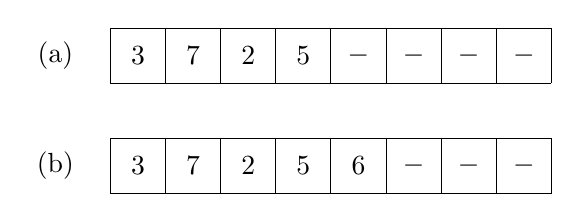
\begin{tikzpicture}[scale=0.7]
\begin{scope}
\draw (0,0) grid (8,1);
\node at (-1,0.5) {(a)};
\node at (0.5,0.5) {$3$};
\node at (1.5,0.5) {$7$};
\node at (2.5,0.5) {$2$};
\node at (3.5,0.5) {$5$};
\node at (4.5,0.5) {$-$};
\node at (5.5,0.5) {$-$};
\node at (6.5,0.5) {$-$};
\node at (7.5,0.5) {$-$};
\end{scope}
\begin{scope}[yshift=-2cm]
\draw (0,0) grid (8,1);
\node at (-1,0.5) {(b)};
\node at (0.5,0.5) {$3$};
\node at (1.5,0.5) {$7$};
\node at (2.5,0.5) {$2$};
\node at (3.5,0.5) {$5$};
\node at (4.5,0.5) {$6$};
\node at (5.5,0.5) {$-$};
\node at (6.5,0.5) {$-$};
\node at (7.5,0.5) {$-$};
\end{scope}
\end{tikzpicture}
\caption{(a) Lista $[3,7,2,5]$ tallennettuna taulukkoon. (b) Listan loppuun lisätään alkio 6.}
\label{fig:listau}
\end{figure}

\begin{figure}
\center
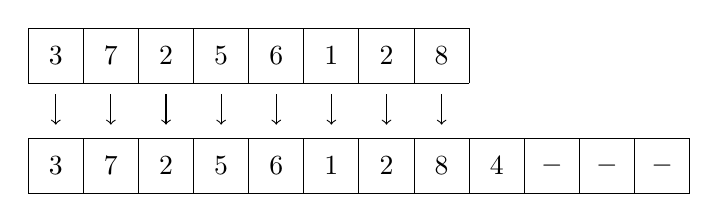
\begin{tikzpicture}[scale=0.7]
\begin{scope}
\draw (0,0) grid (8,1);
\node at (0.5,0.5) {$3$};
\node at (1.5,0.5) {$7$};
\node at (2.5,0.5) {$2$};
\node at (3.5,0.5) {$5$};
\node at (4.5,0.5) {$6$};
\node at (5.5,0.5) {$1$};
\node at (6.5,0.5) {$2$};
\node at (7.5,0.5) {$8$};
\foreach \x in {0,...,7} \draw[->] (\x+0.5,-0.2) -- (\x+0.5,-0.75);
\end{scope}
\begin{scope}[yshift=-2cm]
\draw (0,0) grid (12,1);
\node at (0.5,0.5) {$3$};
\node at (1.5,0.5) {$7$};
\node at (2.5,0.5) {$2$};
\node at (3.5,0.5) {$5$};
\node at (4.5,0.5) {$6$};
\node at (5.5,0.5) {$1$};
\node at (6.5,0.5) {$2$};
\node at (7.5,0.5) {$8$};
\node at (8.5,0.5) {$4$};
\node at (9.5,0.5) {$-$};
\node at (10.5,0.5) {$-$};
\node at (11.5,0.5) {$-$};
\end{scope}
\end{tikzpicture}
\caption{Taulukkoon ei mahdu enää uutta alkiota. Meidän täytyy varata uusi suurempi taulukko
ja kopioida vanhan taulukon sisältö sinne.}
\label{fig:lisuus}
\end{figure}

Mitä tapahtuu sitten, kun jossain vaiheessa koko taulukko
on täynnä eikä uusi listalle lisättävä alkio mahdu enää taulukkoon?
Tällöin täytyy ensin varata uusi suurempi taulukko ja
kopioida kaikki vanhan taulukon alkiot siihen,
minkä jälkeen uusi alkio voidaan lisätä listalle.
Tämä vie aikaa $O(n)$, koska kaikki listan alkiot täytyy kopioida
uuteen paikkaan muistissa.
Esimerkiksi kuvassa \ref{fig:lisuus} uusi alkio 4 ei mahdu taulukkoon,
joten joudumme varaamaan uuden taulukon ja kopioimaan alkiot.

Olemme saaneet siis aikaan listan, jossa lisääminen
vie aikaa \emph{joko} $O(1)$ tai $O(n)$ riippuen siitä,
mahtuuko alkio nykyiseen taulukkoon vai täytyykö
varata uusi taulukko.
Jotta lista olisi käyttökelpoinen, hidas $O(n)$-operaatio
ei saisi esiintyä liian usein.
Osoittautuu, että tämä tavoite toteutuu,
kunhan varaamme uuden taulukon aina reilusti aiempaa suuremmaksi.
Tyypillinen ratkaisu on \emph{kaksinkertaistaa} taulukon koko aina,
kun varaamme uuden taulukon.
Kun toimimme näin, jokaisen alkion lisääminen listalle vie
\emph{keskimäärin} vain $O(1)$ aikaa.

Miksi aikaa kuluu keskimäärin vain $O(1)$?
Tarkastellaan tilannetta, jossa listassa on $n$ alkiota
ja taulukko on tullut täyteen,
joten alkiot täytyy kopioida uuteen taulukkoon.
Tiedämme, että alkioita kopioitiin viimeksi silloin,
kun listassa oli $n/2$ alkiota,
joten listaan on lisätty välissä $n/2$ alkiota tehokkaasti.
Niinpä $n$ alkion kopioimisen kustannus voidaan jakaa
$n/2$ aiemmin lisätylle alkiolle, ja jokaiseen alkioon
kohdistuva lisäkustannus on vakio.
Taulukon kasvattamisen vaikutus kokonaisuuteen on siis pieni.

\begin{figure}
\center
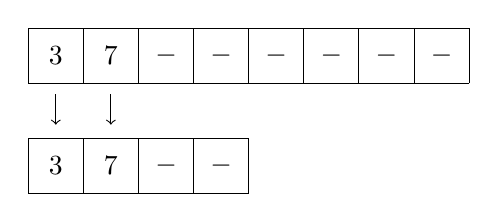
\begin{tikzpicture}[scale=0.7]
\begin{scope}
\draw (0,0) grid (8,1);
\node at (0.5,0.5) {$3$};
\node at (1.5,0.5) {$7$};
\node at (2.5,0.5) {$-$};
\node at (3.5,0.5) {$-$};
\node at (4.5,0.5) {$-$};
\node at (5.5,0.5) {$-$};
\node at (6.5,0.5) {$-$};
\node at (7.5,0.5) {$-$};
\foreach \x in {0,...,1} \draw[->] (\x+0.5,-0.2) -- (\x+0.5,-0.75);
\end{scope}
\begin{scope}[yshift=-2cm]
\draw (0,0) grid (4,1);
\node at (0.5,0.5) {$3$};
\node at (1.5,0.5) {$7$};
\node at (2.5,0.5) {$-$};
\node at (3.5,0.5) {$-$};
\end{scope}
\end{tikzpicture}
\caption{Poistojen jälkeen taulukon koko on käynyt tarpeettoman suureksi,
ja puolitamme taulukon koon.}                                                                        
\label{fig:lispoi}
\end{figure}

Voimme poistaa alkion listan lopusta aina $O(1)$-ajassa,
koska taulukon kokoa ei tarvitse koskaan suurentaa.
Tässä voi kuitenkin tulla ongelmaksi, että monien poistojen
jälkeen taulukossa on turhan paljon tyhjää tilaa lopussa.
Voimme soveltaa tässä käänteisesti samaa ideaa kuin lisäämisessä:
jos poistamisen jälkeen vain \emph{neljännes} taulukosta on käytössä,
puolitamme taulukon koon.
Kuva \ref{fig:lispoi} näyttää esimerkin tällaisesta tilanteesta.
Tällä tavalla myös poistamiset vievät keskimäärin aikaa $O(1)$.

Miksi emme voisi varata heti aluksi niin suurta taulukkoa,
että lopullinen lista mahtuisi siihen varmasti?
Tässä olisi huonona puolena, että listan toteutus tuhlaisi muistia.
Algoritmissa saattaa olla samaan aikaan käytössä monia listoja,
ja haluamme, että listalle varattu taulukko on samaa kokoluokkaa
kuin listan todellinen sisältö.

\subsection{Muutokset alussa ja lopussa}

Melko samaan tapaan voimme myös luoda taulukkolistan,
joka sallii tehokkaat alkioiden lisäykset ja poistot
sekä listan alussa että lopussa.
Jotta tämä onnistuisi, muutamme listan tallennustapaa niin,
että lista voi alkaa ja päättyä missä tahansa taulukon
kohdassa ja listan sisältö voi tarvittaessa jatkua taulukon lopusta alkuun.

\begin{figure}
\center
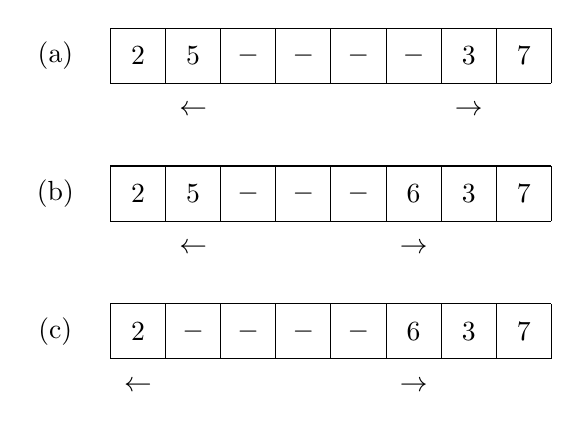
\begin{tikzpicture}[scale=0.7]
\begin{scope}
\draw (0,0) grid (8,1);
\node at (-1,0.5) {(a)};
\node at (0.5,0.5) {$2$};
\node at (1.5,0.5) {$5$};
\node at (2.5,0.5) {$-$};
\node at (3.5,0.5) {$-$};
\node at (4.5,0.5) {$-$};
\node at (5.5,0.5) {$-$};
\node at (6.5,0.5) {$3$};
\node at (7.5,0.5) {$7$};
\node at (1.5,-0.5) {$\leftarrow$};
\node at (6.5,-0.5) {$\rightarrow$};
\end{scope}
\begin{scope}[yshift=-2.5cm]
\draw (0,0) grid (8,1);
\node at (-1,0.5) {(b)};
\node at (0.5,0.5) {$2$};
\node at (1.5,0.5) {$5$};
\node at (2.5,0.5) {$-$};
\node at (3.5,0.5) {$-$};
\node at (4.5,0.5) {$-$};
\node at (5.5,0.5) {$6$};
\node at (6.5,0.5) {$3$};
\node at (7.5,0.5) {$7$};
\node at (1.5,-0.5) {$\leftarrow$};
\node at (5.5,-0.5) {$\rightarrow$};
\end{scope}
\begin{scope}[yshift=-5cm]
\draw (0,0) grid (8,1);
\node at (-1,0.5) {(c)};
\node at (0.5,0.5) {$2$};
\node at (1.5,0.5) {$-$};
\node at (2.5,0.5) {$-$};
\node at (3.5,0.5) {$-$};
\node at (4.5,0.5) {$-$};
\node at (5.5,0.5) {$6$};
\node at (6.5,0.5) {$3$};
\node at (7.5,0.5) {$7$};
\node at (0.5,-0.5) {$\leftarrow$};
\node at (5.5,-0.5) {$\rightarrow$};
\end{scope}
\end{tikzpicture}
\caption{(a) Lista $[3,7,2,5]$ tallennettuna taulukkoon.
(b) Listan alkuun lisätään alkio 6.
(c) Listan lopusta poistetaan alkio 5.}
\label{fig:lismol}
\end{figure}

Kuva \ref{fig:lismol} näyttää esimerkin listan $[3,7,2,5]$
uudesta tallennustavasta.
Merkki $\rightarrow$ osoittaa kohdan, josta lista alkaa,
ja merkki $\leftarrow$ osoittaa kohdan, johon lista päättyy.
Kun haluamme lisätä alkion listan alkuun,
siirrymme vasemmalle kohdasta $\rightarrow$,
ja kun haluamme lisätä alkion listan loppuun,
siirrymme oikealle kohdasta $\leftarrow$.
Kun haluamme poistaa alkioita listasta,
menettelemme käänteisesti.

Jos kohdat $\leftarrow$ ja $\rightarrow$ ovat vierekkäin
tässä järjestyksessä, tämä voi tarkoittaa kahta asiaa:
joko lista on tyhjä tai sitten kaikki taulukon kohdat ovat käytössä.
Kuva \ref{fig:lismol2} näyttää esimerkin näistä tilanteista.
Kun pidämme muistissa alkioiden määrää,
voimme päätellä siitä, kumpi tilanne on kyseessä.
Jos taulukko on täynnä ja haluamme lisätä uuden alkion,
meidän täytyy varata uusi suurempi taulukko, johon listan sisältö siirretään.
Voimme menetellä samalla tavalla kuin aiemmin ja
esimerkiksi kaksinkertaistaa taulukon koon joka vaiheessa,
jolloin operaatiot vievät keskimäärin aikaa $O(1)$.

\begin{figure}
\center
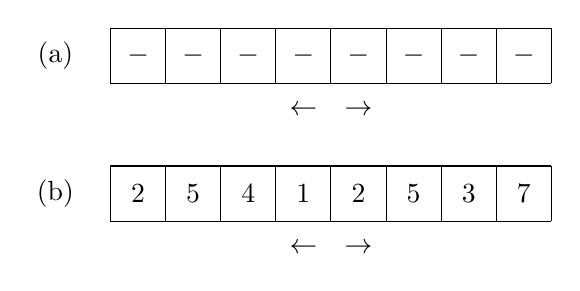
\begin{tikzpicture}[scale=0.7]
\begin{scope}
\draw (0,0) grid (8,1);
\node at (-1,0.5) {(a)};
\node at (0.5,0.5) {$-$};
\node at (1.5,0.5) {$-$};
\node at (2.5,0.5) {$-$};
\node at (3.5,0.5) {$-$};
\node at (4.5,0.5) {$-$};
\node at (5.5,0.5) {$-$};
\node at (6.5,0.5) {$-$};
\node at (7.5,0.5) {$-$};
\node at (3.5,-0.5) {$\leftarrow$};
\node at (4.5,-0.5) {$\rightarrow$};
\end{scope}
\begin{scope}[yshift=-2.5cm]
\draw (0,0) grid (8,1);
\node at (-1,0.5) {(b)};
\node at (0.5,0.5) {$2$};
\node at (1.5,0.5) {$5$};
\node at (2.5,0.5) {$4$};
\node at (3.5,0.5) {$1$};
\node at (4.5,0.5) {$2$};
\node at (5.5,0.5) {$5$};
\node at (6.5,0.5) {$3$};
\node at (7.5,0.5) {$7$};
\node at (3.5,-0.5) {$\leftarrow$};
\node at (4.5,-0.5) {$\rightarrow$};
\end{scope}
\end{tikzpicture}
\caption{Kaksi samantapaista tilannetta:
(a) Listassa ei ole yhtään alkiota.
(b) Listan alkiot täyttävät koko taulukon.}
\label{fig:lismol2}
\end{figure}

\section{Linkitetty lista}

\index{linkitetty lista}

\emph{Linkitetty lista} (\emph{linked list}) muodostuu solmuista, joista jokainen sisältää
yhden listan alkion.
Linkitetty lista voi olla yhteen tai kahteen suuntaan linkitetty.
Yhteen suuntaan linkitetyssä listassa jokaisesta solmusta
on viittaus seuraavaan solmuun, ja kahteen suuntaan linkitetyssä
listassa jokaisesta solmusta on viittaus sekä seuraavaan että edelliseen solmuun.

\begin{figure}
\center
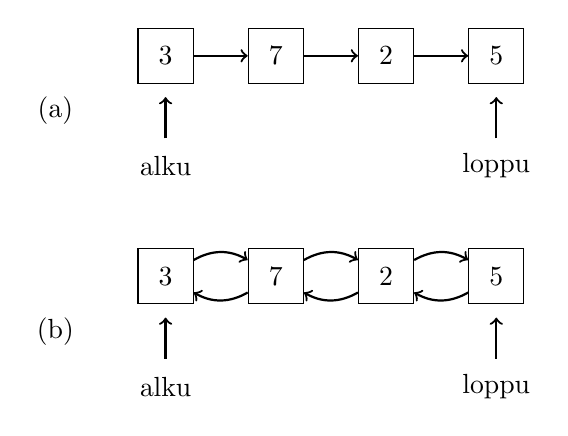
\begin{tikzpicture}[scale=0.7]
\begin{scope}
\node[draw, rectangle, minimum size=7mm] (1) at (0,0) {$3$};
\node[draw, rectangle, minimum size=7mm] (2) at (2,0) {$7$};
\node[draw, rectangle, minimum size=7mm] (3) at (4,0) {$2$};
\node[draw, rectangle, minimum size=7mm] (4) at (6,0) {$5$};
\path[draw,thick,->] (1) -- (2);
\path[draw,thick,->] (2) -- (3);
\path[draw,thick,->] (3) -- (4);
\node at (0,-2) {alku};
\node at (6,-2) {loppu};
\path[draw,thick,->] (0,-1.5) -- (0,-0.75);
\path[draw,thick,->] (6,-1.5) -- (6,-0.75);
\node at (-2,-1) {(a)};
\end{scope}
\begin{scope}[yshift=-4cm]
\node[draw, rectangle, minimum size=7mm] (1) at (0,0) {$3$};
\node[draw, rectangle, minimum size=7mm] (2) at (2,0) {$7$};
\node[draw, rectangle, minimum size=7mm] (3) at (4,0) {$2$};
\node[draw, rectangle, minimum size=7mm] (4) at (6,0) {$5$};
\path[draw,thick,->] (1) edge [bend left] (2);
\path[draw,thick,->] (2) edge [bend left] (3);
\path[draw,thick,->] (3) edge [bend left] (4);
\path[draw,thick,->] (4) edge [bend left] (3);
\path[draw,thick,->] (3) edge [bend left] (2);
\path[draw,thick,->] (2) edge [bend left] (1);
\node at (0,-2) {alku};
\node at (6,-2) {loppu};
\path[draw,thick,->] (0,-1.5) -- (0,-0.75);
\path[draw,thick,->] (6,-1.5) -- (6,-0.75);
\node at (-2,-1) {(b)};
\end{scope}
\end{tikzpicture}
\caption{Lista $[3,7,2,5]$ linkitettynä listana.
(a) Yhteen suuntaan linkitetty lista. (b) Kahteen suuntaan linkitetty lista.}
\label{fig:linlis}
\end{figure}

Kuva \ref{fig:linlis} näyttää esimerkkinä listan $[3,7,2,5]$
yhteen ja kahteen suuntaan linkitettynä.
Molemmissa listoissa tiedossa on viittaukset listan
alkuun ja loppuun.
Yhteen suuntaan linkitetyssä listassa voimme käydä
läpi listan alkiot alusta loppuun,
kun taas kahteen suuntaan linkitetyssä listassa
voimme kulkea sekä alusta loppuun että lopusta alkuun.

Tavallinen tapa toteuttaa linkitetty rakenne ohjelmointikielissä
on luoda luokka, jonka oliot vastaavat rakenteen solmuja.
Esimerkiksi voisimme rakentaa yhteen suuntaan
linkitetyn listan $[1,2,3]$ tähän tapaan:

\begin{code}
a.arvo = 1
a.seuraava = b
b.arvo = 2
b.seuraava = c
c.arvo = 3
c.seuraava = null
\end{code}

Tässä toteutuksessa jokaisessa solmuoliossa on kaksi kenttää:
\texttt{arvo} on solmussa oleva arvo ja
\texttt{seuraava} viittaa listan seuraavaan solmuun.
Listan loppumisen ilmaisee viimeisessä solmussa oleva arvo \texttt{null}.
Voisimme käydä läpi listan solmut näin:

\begin{code}
s = a
while s != null
    print(s.arvo)
    s = s.seuraava
\end{code}

\subsection{Listan operaatiot}

Käytännössä järkevä tapa toteuttaa linkitetty lista on tehdä
listasta kaksisuuntainen, jolloin tiedämme jokaisessa solmussa
seuraavan ja edellisen solmun ja voimme kulkea listaa molempiin suuntiin.

Linkitetyn listan etuna on,
että voimme lisätä ja poistaa
alkioita $O(1)$-ajassa kaikissa listan kohdissa.
Kun haluamme lisätä listalle alkion,
luomme ensin uuden solmun ja muutamme sitten
sen vieressä olevien solmujen viittauksia niin,
että ne viittaavat uuteen solmuun.
Vastaavasti kun haluamme poistaa alkion,
muutamme viittauksia niin, että solmu ohitetaan.

\begin{figure}
\center
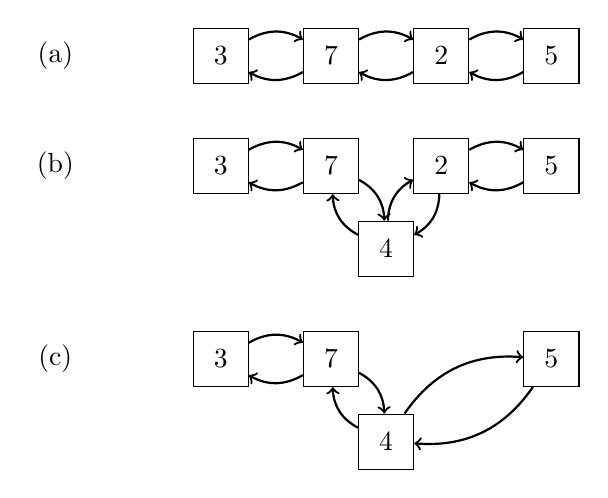
\begin{tikzpicture}[scale=0.7]
\begin{scope}
\node at (-3,0) {(a)};
\node[draw, rectangle, minimum size=7mm] (1) at (0,0) {$3$};
\node[draw, rectangle, minimum size=7mm] (2) at (2,0) {$7$};
\node[draw, rectangle, minimum size=7mm] (3) at (4,0) {$2$};
\node[draw, rectangle, minimum size=7mm] (4) at (6,0) {$5$};
\path[draw,thick,->] (1) edge [bend left] (2);
\path[draw,thick,->] (2) edge [bend left] (3);
\path[draw,thick,->] (3) edge [bend left] (4);
\path[draw,thick,->] (4) edge [bend left] (3);
\path[draw,thick,->] (3) edge [bend left] (2);
\path[draw,thick,->] (2) edge [bend left] (1);
\end{scope}
\begin{scope}[yshift=-2cm]
\node at (-3,0) {(b)};
\node[draw, rectangle, minimum size=7mm] (1) at (0,0) {$3$};
\node[draw, rectangle, minimum size=7mm] (2) at (2,0) {$7$};
\node[draw, rectangle, minimum size=7mm] (3) at (4,0) {$2$};
\node[draw, rectangle, minimum size=7mm] (4) at (6,0) {$5$};
\node[draw, rectangle, minimum size=7mm] (5) at (3,-1.5) {$4$};
\path[draw,thick,->] (1) edge [bend left] (2);
\path[draw,thick,->] (2) edge [bend left] (5);
\path[draw,thick,->] (5) edge [bend left] (3);
\path[draw,thick,->] (3) edge [bend left] (4);
\path[draw,thick,->] (4) edge [bend left] (3);
\path[draw,thick,->] (3) edge [bend left] (5);
\path[draw,thick,->] (5) edge [bend left] (2);
\path[draw,thick,->] (2) edge [bend left] (1);
\end{scope}
\begin{scope}[yshift=-5.5cm]
\node at (-3,0) {(c)};
\node[draw, rectangle, minimum size=7mm] (1) at (0,0) {$3$};
\node[draw, rectangle, minimum size=7mm] (2) at (2,0) {$7$};
\node[draw, rectangle, minimum size=7mm] (4) at (6,0) {$5$};
\node[draw, rectangle, minimum size=7mm] (5) at (3,-1.5) {$4$};
\path[draw,thick,->] (1) edge [bend left] (2);
\path[draw,thick,->] (2) edge [bend left] (5);
\path[draw,thick,->] (5) edge [bend left] (4);
\path[draw,thick,->] (4) edge [bend left] (5);
\path[draw,thick,->] (5) edge [bend left] (2);
\path[draw,thick,->] (2) edge [bend left] (1);
\end{scope}
\end{tikzpicture}
\caption{(a) Alkuperäinen lista $[3,7,2,5]$.
(b) Listan keskelle lisätään alkio $4$.
(c) Listasta poistetaan alkio $2$.}
\label{fig:lismuu}
\end{figure}

Kuva \ref{fig:lismuu} näyttää esimerkin linkitetyn listan käsittelystä.
Listan sisältönä on aluksi $[3,7,2,5]$.
Sitten lisämme listan keskelle alkion 4,
jolloin luomme ensin uuden solmun alkiolle ja muutamme
sitten viittauksia alkioiden 7 ja 2 välillä niin,
että alkio 4 tulee niiden väliin.
Lopuksi poistamme listasta alkion 2, jolloin yhdistämme
alkiot 4 ja 5 suoraan toisiinsa.

Pääsemme listan ensimmäiseen ja viimeiseen solmuun tehokkaasti,
koska muistissa on viittaukset niihin.
Sen sijaan jos haluamme päästä johonkin muuhun listan kohtaan,
matka täytyy aloittaa listan alusta tai lopusta ja kulkea askel
kerrallaan viittauksia seuraten.
Niinpä listan keskellä olevaan kohtaan pääseminen vie aikaa $O(n)$.
Joudumme liikkumaan solmuihin linkkejä pitkin, koska solmut voivat
olla eri puolilla muistia eikä ole keinoa tietää suoraan,
mihin mikäkin solmu on tallennettu.

\subsection{Listojen vertailua}

\begin{table}
\center
\begin{tabular}{lrr}
operaatio & taulukkolista & linkitetty lista \\
\hline
pääsy listan alkuun & $O(1)$ & $O(1)$ \\
pääsy listan loppuun & $O(1)$ & $O(1)$ \\ 
pääsy listan keskelle &  $O(1)$ & $O(n)$ \\
lisäys/poisto listan alussa & $O(1)$ & $O(1)$ \\
lisäys/poisto listan lopussa & $O(1)$ & $O(1)$ \\ 
lisäys/poisto listan keskellä &  $O(n)$ & $O(1)$ \\
\end{tabular}
\caption{Taulukkolistan ja linkitetyn listan aikavaativuuksia.}
\label{tab:taulin}
\end{table}

Taulukko \ref{tab:taulin} esittää yhteenvedon taulukkolistan ja
linkitetyn listan ominaisuuksista.
Kummassakin toteutuksessa on yksi operaatio,
joka ei ole tehokas.
Taulukkolistassa pääsemme tehokkaasti mihin tahansa listan
kohtaan, mutta on hidasta muokata listaa keskeltä.
Linkitetyssä listassa voimme helposti muokata listaa mistä tahansa,
mutta keskelle pääseminen on hidasta.

Huomaa, että keskelle pääsemisen hitaus rajoittaa melko paljon
linkitetyn listan käyttämistä.
Vaikka pystymme sinänsä muokkaamaan listaa mistä tahansa kohdasta
tehokkaasti, meidän tulee ensin \emph{päästä} kyseiseen kohtaan.
Jos jostain syystä on etukäteen tiedossa viittaus listan keskelle,
voimme muokata kyseistä kohtaa tehokkaasti,
mutta muuten tulee ensin kulkea haluttuun kohtaan,
missä kuluu aikaa $O(n)$.

\section{Pino ja jono}

Listan avulla voimme toteuttaa myös kaksi erikoistunutta tietorakennetta,
pinon ja jonon, jotka sisältävät vain osan listan ominaisuuksista
eli niiden operaatiot ovat listaa rajoittuneempia.

\begin{figure}
\center
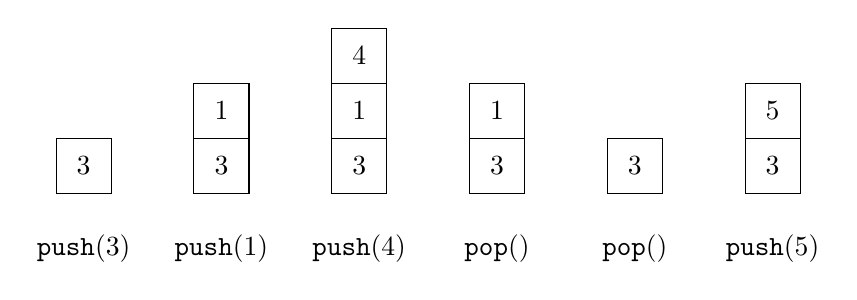
\begin{tikzpicture}[scale=0.7]
\begin{scope}[xshift=2.5cm]
\draw (0,0) grid (1,1);
\node at (0.5,0.5) {3};
\node at (0.5,-1) {$\texttt{push}(3)$};
\end{scope}
\begin{scope}[xshift=5cm]
\draw (0,0) grid (1,2);
\node at (0.5,0.5) {3};
\node at (0.5,1.5) {1};
\node at (0.5,-1) {$\texttt{push}(1)$};
\end{scope}
\begin{scope}[xshift=7.5cm]
\draw (0,0) grid (1,3);
\node at (0.5,0.5) {3};
\node at (0.5,1.5) {1};
\node at (0.5,2.5) {4};
\node at (0.5,-1) {$\texttt{push}(4)$};
\end{scope}
\begin{scope}[xshift=10cm]
\draw (0,0) grid (1,2);
\node at (0.5,0.5) {3};
\node at (0.5,1.5) {1};
\node at (0.5,-1) {$\texttt{pop}()$};
\end{scope}
\begin{scope}[xshift=12.5cm]
\draw (0,0) grid (1,1);
\node at (0.5,0.5) {3};
\node at (0.5,-1) {$\texttt{pop}()$};
\end{scope}
\begin{scope}[xshift=15cm]
\draw (0,0) grid (1,2);
\node at (0.5,0.5) {3};
\node at (0.5,1.5) {5};
\node at (0.5,-1) {$\texttt{push}(5)$};
\end{scope}
\end{tikzpicture}
\caption{Esimerkki pinon käsittelystä:
lisäämme tyhjään pinoon alkiot 3, 1 ja 4, poistamme kaksi ylintä
alkiota ja lisäämme lopuksi alkion 5.}
\label{fig:pinesi}
\end{figure}

\begin{figure}
\center
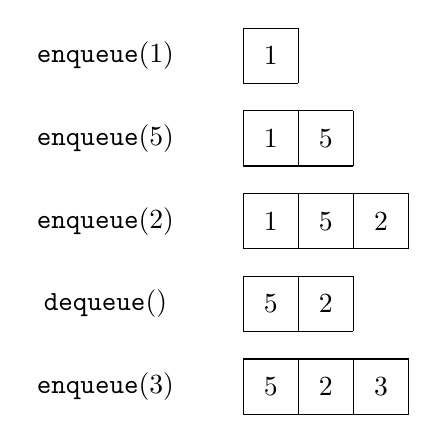
\begin{tikzpicture}[scale=0.7]
\begin{scope}
\draw (0,0) grid (1,1);
\node at (0.5,0.5) {$1$};
\node at (-2.5,0.5) {$\texttt{enqueue}(1)$};
\end{scope}
\begin{scope}[yshift=-1.5cm]
\draw (0,0) grid (2,1);
\node at (0.5,0.5) {$1$};
\node at (1.5,0.5) {$5$};
\node at (-2.5,0.5) {$\texttt{enqueue}(5)$};
\end{scope}
\begin{scope}[yshift=-3cm]
\draw (0,0) grid (3,1);
\node at (0.5,0.5) {$1$};
\node at (1.5,0.5) {$5$};
\node at (2.5,0.5) {$2$};
\node at (-2.5,0.5) {$\texttt{enqueue}(2)$};
\end{scope}
\begin{scope}[yshift=-4.5cm]
\draw (0,0) grid (2,1);
\node at (0.5,0.5) {$5$};
\node at (1.5,0.5) {$2$};
\node at (-2.5,0.5) {$\texttt{dequeue}()$};
\end{scope}
\begin{scope}[yshift=-6cm]
\draw (0,0) grid (3,1);
\node at (0.5,0.5) {$5$};
\node at (1.5,0.5) {$2$};
\node at (2.5,0.5) {$3$};
\node at (-2.5,0.5) {$\texttt{enqueue}(3)$};
\end{scope}
\end{tikzpicture}
\caption{Esimerkki jonon käsittelystä:
lisäämme tyhjään jonon alkiot 1, 5 ja 2,
poistamme yhden alkion ja lisäämme vielä alkion 3.}
\label{fig:jonesi}
\end{figure}

\index{pino}

\emph{Pino} (\emph{stack}) on tietorakenne,
jonka operaatiot ovat
alkion lisääminen pinon päälle (\texttt{push}),
ylimmän alkion poistaminen (\texttt{pop})
sekä ylimmän alkion hakeminen.
Esimerkiksi kuvassa \ref{fig:pinesi} lisäämme ensin tyhjään pinoon kolme alkiota,
poistamme sitten kaksi alkiota ja lisäämme vielä yhden alkion.

\index{jono}

\emph{Jono} (\emph{queue}) on tietorakenne, jossa voimme lisätä alkioita
jonon loppuun (\texttt{enqueue}),
poistaa alkioita jonon alusta (\texttt{dequeue})
ja hakea alkioita molemmista päistä.
Esimerkiksi kuvassa \ref{fig:jonesi} lisäämme ensin tyhjään jonoon
kolme alkiota, poistamme sitten yhden alkion ja lisämme vielä yhden alkion.

Pystymme toteuttamaan sekä pinon että jonon helposti
listana niin, että niiden operaatiot toimivat ajassa $O(1)$.
Mutta mitä järkeä on luoda uusia tietorakenteita,
jotka ovat \emph{huonompia} kuin lista?
Listassa voimme käsitellä mitä tahansa alkioita, mutta
pinossa ja jonossa emme pääse käsiksi keskellä oleviin alkioihin.
Selitys on siinä, että pino ja jono ovat hyödyllisiä 
\emph{käsit\-teitä} algoritmien suunnittelussa.
Voimme usein ajatella algoritmissa tarvittavaa
tietorakennetta pinona tai jonona ja toteuttaa sen sitten listana.

Tarkastellaan esimerkkinä ongelmaa, jossa annettuna on
$n$ merkin pituinen \emph{sulkulauseke}, 
joka muodostuu kaarisulkeista \texttt{(} ja \texttt{)} sekä
hakasulkeista \texttt{[} ja \texttt{]}.
Haluamme selvittää, onko lauseke \emph{oikein muodostettu} eli
onko jokaiselle aloittavalle sululle vastaava lopettava pari.
Esimerkiksi lauseke \texttt{[()]()} on oikein muodostettu,
kun taas lauseke \texttt{[()(])} ei ole.
Voimme ratkaista ongelman $O(n)$-ajassa pinon avulla
käymällä läpi lausekkeen merkit vasemmalta oikealle.
Kun vastaan tulee aloittava sulku \texttt{(} tai \texttt{[},
lisäämme sen pinoon.
Kun taas vastaan tulee lopettava sulku \texttt{)} tai \texttt{]},
tutkimme, mikä on pinossa ylimpänä oleva merkki.
Jos merkki on vastaava aloittava sulku,
poistamme sen pinosta, ja muuten toteamme, että lauseke on virheellinen.
Jos lausekkeen läpikäynnin aikana ei esiinny virheitä
ja pino on lopuksi tyhjä, lauseke on oikein muodostettu.

\section{Ohjelmointikielten toteutukset}

\subsection{Java}

Javan \texttt{ArrayList} on taulukkolista,
jossa alkion lisääminen ja poistaminen on tehokasta,
kun se tapahtuu listan lopussa.
Metodi \texttt{add} lisää tehokkaasti alkion listan loppuun:

\begin{code}
ArrayList<Integer> lista = new ArrayList<>();
lista.add(1);
lista.add(2);
lista.add(3);
// tulos: [1,2,3]
\end{code}

Metodi \texttt{remove} poistaa alkion
annetusta listan kohdasta.
Metodi toimii tehokkaasti, kun poistokohta on listan lopussa.
Esimerkiksi seuraava koodi poistaa listan viimeisen alkion:

\begin{code}
lista.remove(lista.size()-1);
\end{code}

Koska lista on tallennettu taulukkona,
pääsemme myös tehokkaasti käsiksi missä tahansa kohdassa
olevaan alkioon metodeilla \texttt{get} ja \texttt{set}:

\begin{code}
// hae alkio kohdasta 3
int x = lista.get(3);
// muuta kohdan 5 alkioksi 8
lista.set(5,8);
\end{code}

\texttt{ArrayDeque} on taulukkolista,
joka sallii tehokkaat lisäykset ja poistot
sekä listan alussa että lopussa.
Metodit \texttt{addFirst} ja \texttt{addLast}
lisäävät alkioita,
ja metodit \texttt{removeFirst} ja \texttt{removeLast}
poistavat alkioita.

\begin{code}
ArrayDeque<Integer> lista = new ArrayDeque<>();
lista.addLast(1);
lista.addLast(2);
lista.addLast(3);
lista.removeFirst();
lista.addFirst(4);
// tulos: [4,2,3]
\end{code}

Lisäksi voimme hakea listan ensimmäisen ja viimeisen alkion
metodeilla \texttt{getFirst} ja \texttt{getLast}:

\begin{code}
int eka = lista.getFirst();
int vika = lista.getLast();
\end{code}

Rajoituksena on kuitenkin, että yleisiä metodeita
\texttt{get} ja \texttt{set} ei ole tarjolla
eli emme pääse tehokkaasti käsiksi listan keskellä
oleviin alkioihin.

\texttt{LinkedList} on kaksisuuntainen linkitetty lista,
jota voimme käsitellä samaan tapaan kuin \texttt{ArrayDeque}-listaa:

\begin{code}
LinkedList<Integer> lista = new LinkedList<>();
lista.addLast(1);
lista.addLast(2);
lista.addLast(3);
lista.removeFirst();
lista.addFirst(4);
// tulos: [4,2,3]
\end{code}

\texttt{LinkedList} tarjoaa myös metodit
\texttt{get} ja \texttt{set}, joiden avulla
pääsee käsiksi tietyssä kohdassa listalla olevaan alkioon.
Nämä metodit vievät kuitenkin aikaa $O(n)$,
koska joudumme kulkemaan ensin oikeaan kohtaan listan
alusta tai lopusta.

\index{iteraattori}

Voimme käsitellä listaa myös \emph{iteraattorilla}
(\emph{iterator}),
joka osoittaa tiettyyn listan kohtaan.
Esimerkiksi seuraava koodi luo iteraattorin,
joka osoittaa listan alkuun,
siirtää iteraattoria kaksi askelta eteenpäin ja
lisää alkion iteraattorin kohdalle eli listan
toisen ja kolmannen alkion väliin.

\begin{code}
ListIterator<Integer> x = lista.listIterator();
x.next();
x.next();
x.add(5);
\end{code}

Iteraattorin avulla voimme muokata tehokkaasti
linkitettyä listaa siitä kohdasta,
jossa iteraattori on tällä hetkellä.

\subsection{Python}

Pythonin tavallinen lista on taulukkolista,
jota voi käsitellä tehokkaasti listan lopusta.
Metodi \texttt{append} lisää alkion listan loppuun:

\begin{code}
lista = []
lista.append(1)
lista.append(2)
lista.append(3)
# tulos: [1,2,3]
\end{code}

Metodi \texttt{pop} puolestaan poistaa listan viimeisen alkion:

\begin{code}
lista.pop()
\end{code}

Pääsemme käsiksi listan alkioihin tehokkaasti \texttt{[]}-syntaksin avulla:

\begin{code}
x = lista[3]
lista[5] = 8
\end{code}

Pythonissa on myös lista \texttt{deque},
joka on toteutettu linkitettynä listana.
Lisäykset ja poistot ovat tehokkaita sekä listan
alussa että lopussa.
Saamme tietorakenteen käyttöön näin:

\begin{code}
from collections import deque
\end{code}

Tavallisen listan tavoin \texttt{deque} tarjoaa
metodit \texttt{append} ja \texttt{pop},
mutta lisäksi siinä on metodit \texttt{appendleft}
ja \texttt{popleft}, joiden avulla voi lisätä ja poistaa
alkioita listan alussa:

\begin{code}
lista = deque()
lista.append(1)
lista.append(2)
lista.append(3)
lista.popleft()
lista.appendleft(4)
# tulos: [4,2,3]
\end{code}

Listan alkuun ja loppuun pääsee käsiksi näin:

\begin{code}
eka = lista[0]
vika = lista[-1]
\end{code}

Myös listan keskellä olevia alkioita voi käsitellä \texttt{[]}-syntaksilla,
mutta tämä vie aikaa $O(n)$, koska kyseessä on linkitetty lista.

\section{Miten valita lista?}

Voimme käyttää usein algoritmin toteutukseen joko
taulukkolistaa tai linkitettyä listaa ja saada aikaan
aikavaativuuden kannalta yhtä tehokkaan algoritmin.
Esimerkiksi jos algoritmi lisää listan loppuun alkioita,
sekä taulukkolistassa että linkitetyssä listassa
lisäämisen aikavaativuus on $O(1)$.
Mutta kumpi lista on parempi valinta käytännössä?

\begin{figure}
\center
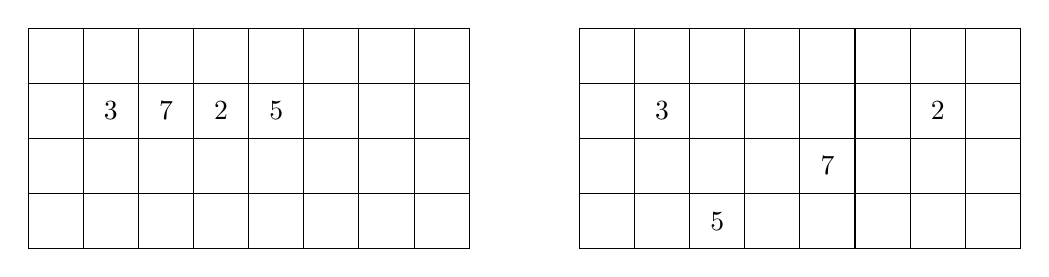
\begin{tikzpicture}[scale=0.7]
\begin{scope}
\draw (0,0) grid (8,4);
\node at (1.5,2.5) {3};
\node at (2.5,2.5) {7};
\node at (3.5,2.5) {2};
\node at (4.5,2.5) {5};
\end{scope}
\begin{scope}[xshift=10cm]
\draw (0,0) grid (8,4);
\node at (1.5,2.5) {3};
\node at (4.5,1.5) {7};
\node at (6.5,2.5) {2};
\node at (2.5,0.5) {5};
\end{scope}
\end{tikzpicture}
\caption{Taulukkolista ja linkitetty lista tietokoneen muistissa.}
\label{fig:taulin}
\end{figure}

Useimmissa tapauksissa parempi valinta on taulukkolista,
koska nykyaikaiset tietokoneet
\emph{suosivat} taulukkolistan käyttämistä linkitetyn listan sijaan.
Kuvassa \ref{fig:taulin} näkyy, miten taulukkolista ja linkitetty lista
asettuvat tietokoneen muistissa.
Taulukkolistan alkiot ovat peräkkäin, kun taas linkitetyn
listan alkiot voivat olla eri puolilla muistia sekalaisessa
järjestyksessä.
Nykyaikaisen prosessorin välimuistit ja seuraavaksi suoritettavien
komentojen ennustus
on toteutettu niin, että ne ovat parhaimmillaan silloin,
kun tieto on tallennettu muistissa peräkkäin -- eli juuri kuten
taulukkolistassa.
Tämä näkyy käytännössä siinä, että taulukkolistan käsittely on selvästi
tehokkaampaa kuin linkitetyn listan käsittely.

Vaikka linkitetty lista ei ole usein käytännössä hyvä tietorakenne,
linkitetyn rakenteen idea on hyödyllinen
ja tarvitsemme sitä myöhemmin monimutkaisemmissa tietorakenteissa.

\chapter{Hajautustaulu}

\index{hajautustaulu}

\emph{Hajautustaulu} (\emph{hash table}) on tietorakenne,
joka tarjoaa tehokkaat operaatiot alkion lisäämiseen,
hakemiseen ja poistamiseen.
Voimme toteuttaa hajautustaulun avulla \emph{joukon},
jossa on kokoelma alkioita, sekä \emph{hakemiston},
joka sisältää avain-arvo-pareja.

Yksi tapa ajatella hajautusta on, että yleistämme taulukon ideaa:
taulukossa indeksit ovat aina 0, 1, 2, jne., mutta hajautustaulussa
voimme käyttää indeksien sijasta vaikkapa merkkijonoja.
Tämä onnistuu käyttämällä hajautusfunktiota,
joka muuttaa muun tyyppisen alkion indeksiksi,
jotta löydämme sille paikan taulukosta.

\section{Hajautustaulun toteutus}

\index{hajautusfunktio}
\index{hajautusarvo}

Hajautustaulun perustana on \emph{hajautusfunktio}
(\emph{hash function}) $f(x)$,
joka antaa \emph{hajautusarvon} (\emph{hash value})
mille tahansa alkiolle $x$.
Hajautusarvo on kokonaisluku väliltä $0,1,\dots,N-1$,
missä $N$ on hajautustaulun koko.
Hajautusarvo määrää, mihin hajautustaulun kohtaan
alkio tallennetaan.

Tarkastellaan esimerkkinä hajautusfunktiota $f(x)=x \bmod N$,
missä $x$ on kokonaisluku.
Tämä hajautusfunktio antaa hajautusarvoksi luvun $x$
jakojäännöksen $N$:llä.
Esimerkiksi kun $N=10$ ja tallennamme hajautustauluun luvun 14,
saamme sen hajautusarvoksi $f(14)=4$.
Tämä tarkoittaa, että luvun paikka hajautustaulussa on kohdassa 4.
Vastaavasti $f(21)=1$, eli luvun 21 paikka hajautustaulussa on
kohdassa 1.
Kun $N=10$, luvun hajautusarvo on tässä tapauksessa siis
luvun viimeinen numero.

\index{törmäys}

Yleensä hajautustaulun koko $N$ on selvästi pienempi kuin
mahdollisten alkioiden määrä ja
hajautuksessa voi tapahtua \emph{törmäys} (\emph{collision})
eli kahdelle alkiolle tulee sama hajautusarvo.
Esimerkiksi $f(14)=f(24)=4$ eli luvut 14 ja 24 kuuluvat
samaan paikkaan hajautustaulussa.
Tämän vuoksi hajautustaulun toteutuksessa täytyy päättää,
miten tör\-mäykset käsitellään.
Kaksi tavallista tapaa tähän ovat ketjuhajautus sekä avoin hajautus.

\subsection{Ketjuhajautus}

\begin{figure}
\center
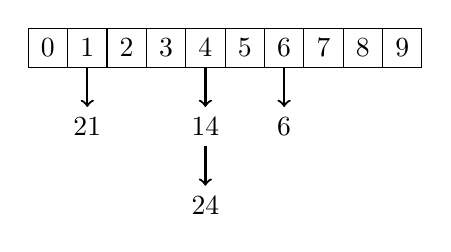
\begin{tikzpicture}[scale=0.5]
\draw (0,0) grid (10,1);
\foreach \x in {0,1,...,9} \node at (0.5+\x,0.5) {\x};
\draw[->,thick] (1.5,0) -- (1.5,-1);
\draw[->,thick] (6.5,0) -- (6.5,-1);
\draw[->,thick] (4.5,0) -- (4.5,-1);
\draw[->,thick] (4.5,-2) -- (4.5,-3);
\node at (1.5,-1.5) {$21$};
\node at (6.5,-1.5) {$6$};
\node at (4.5,-1.5) {$14$};
\node at (4.5,-3.5) {$24$};
\end{tikzpicture}
\caption{Ketjuhajautusta käyttävä hajautustaulu, joka vastaa joukkoa $\{6,14,21,24\}$.
Hajautusfunktiona on $f(x)=x \bmod N$.}
\label{fig:hajtau}
\end{figure}

\index{ketjuhajautus}

\emph{Ketjuhajautus} (\emph{chaining})
on hajautustaulun toteutustapa, jossa jokainen hajautustaulun kohta
sisältää listan alkioista,
joilla on kyseinen hajautusarvo.
Tällöin mahdolliset alkioiden törmäykset eivät haittaa,
koska listoissa voi olla mikä tahansa määrä alkioita.

Kuvassa \ref{fig:hajtau} on esimerkkinä
ketjuhajautusta käyttävä hajautustaulu,
johon on tallennettu joukko $\{6,14,21,24\}$
käyttäen hajautusfunktiota $f(x)=x \bmod N$.
Kohdassa 1 on alkio 21, kohdassa 4 on alkiot 14 ja 24
ja kohdassa 6 on alkio 6.
Muissa kohdissa olevat listat ovat vielä tyhjiä.

Kun haluamme tarkastaa, onko joukossa alkiota $x$,
laskemme ensin sen hajautusarvon $f(x)$.
Tämän jälkeen käymme läpi kaikki kohdan $f(x)$
listassa olevat alkiot ja tarkastamme,
onko jokin niistä alkio $x$.
Vastaavasti kun haluamme lisätä alkion $x$ joukkoon
tai poistaa alkion $x$ joukosta,
teemme muutoksen kohdassa $f(x)$ olevaan listaan.

\begin{figure}
\center
\begin{tikzpicture}[scale=0.5]
\begin{scope}
\draw (0,0) grid (10,1);
\foreach \x in {0,1,...,9} \node at (0.5+\x,0.5) {\x};
\draw[->,thick] (1.5,0) -- (1.5,-1);
\draw[->,thick] (4.5,0) -- (4.5,-1);
\draw[->,thick] (5.5,0) -- (5.5,-1);
\draw[->,thick] (8.5,0) -- (8.5,-1);
\node at (1.5,-1.5) {$14$};
\node at (4.5,-1.5) {$21$};
\node at (5.5,-1.5) {$6$};
\node at (8.5,-1.5) {$24$};
\end{scope}
\begin{scope}[xshift=12cm]
\draw (0,0) grid (10,1);
\foreach \x in {0,1,...,9} \node at (0.5+\x,0.5) {\x};
\draw[->,thick] (3.5,0) -- (3.5,-1);
\draw[->,thick] (3.5,-2) -- (3.5,-3);
\draw[->,thick] (3.5,-4) -- (3.5,-5);
\draw[->,thick] (3.5,-6) -- (3.5,-7);
\node at (3.5,-1.5) {$21$};
\node at (3.5,-3.5) {$14$};
\node at (3.5,-5.5) {$24$};
\node at (3.5,-7.5) {$6$};
\end{scope}
\end{tikzpicture}
\caption{Kaksi hajautustaulua joukolle $\{6,14,21,24\}$.
Vasen tilanne on paras mahdollinen, oikea tilanne taas
huonoin mahdollinen.}
\label{fig:hajjak}
\end{figure}

Ketjuhajautuksessa
hajautustaulun operaatioiden aikavaativuus on $O(m)$,
missä $m$ on listan alkioiden määrä.
Hajautustaulu toimii siis tehokkaasti, jos
siinä olevat listat ovat lyhyitä.
Tämä toteutuu, jos käytetty hajautusfunktio sijoittaa
alkioita tasaisesti hajautustaulun eri puolille.
Kuvassa \ref{fig:hajjak} on kaksi ääriesimerkkiä
hajautuksen onnistumisesta erilaisilla hajautusfunktioilla.
Vasemmassa hajautustaulussa jokainen alkio on eri listassa,
mikä on paras mahdollinen tilanne.
Oikeassa hajautustaulussa kaikki alkiot ovat puolestaan samassa listassa,
mikä on huonoin mahdollinen tilanne.

\subsection{Avoin hajautus}

\index{avoin hajautus}

Toinen tapa toteuttaa hajautustaulu on \emph{avoin hajautus}
(\emph{open addressing}),
jossa alkiot tallennetaan suoraan hajautustauluun listojen sijasta.
Kuitenkin jos alkio kuuluisi paikkaan, jossa on jo valmiina
jokin toinen alkio, sille valitaan toinen paikka jonkin säännön perusteella.

\index{kokeilufunktio}
\index{lineaarinen kokeilu}

Avoimessa hajautuksessa alkion paikkaa hajautustaulussa etsitään
\emph{kokeilufunktiolla} (\emph{probe function})
$h(x,i)$, jossa $x$ on alkio ja $i$ ilmaisee, montako kertaa
sille on yritetty etsiä paikkaa.
Tarkastelemme seuraavaksi yksinkertaista kokeilufunktiota
\[ h(x,i) = (f(x)+i) \bmod N,\]
mikä tarkoittaa, että alkiolle etsitään paikkaa sen
hajautusarvon $f(x)$ antamasta kohdasta lähtien kulkemalla taulukossa oikealle,
kunnes vapaa paikka löytyy.
Tämän menetelmän nimi on \emph{lineaarinen kokeilu}
(\emph{linear probing}).

Kuvassa \ref{fig:hajavo} näkyy joukon $\{6,14,21,24\}$
sijoittuminen hajautustauluun
käyttäen hajautusfunktiota $f(x)=x \bmod N$ ja lineaarista kokeilua.
Tässä alkio 14 on lisätty ennen alkiota 24,
minkä vuoksi alkio 14 on sen hajautusarvon mukaisessa kohdassa 4
mutta alkio 24 on kohdassa 5, koska kohta 4 oli jo varattu.
Kuvassa \ref{fig:hajav2} mukaan lisätään vielä alkio 44,
jolla on myös hajautusarvo 4.
Koska kohdissa 4, 5 ja 6 on jo alkio, alkion 44 kohdaksi tulee 7.
Alkio voi sijoittua siis kauaskin hajautusarvon määräämästä kohdasta,
jos hajautustaulussa on täyttä.

\begin{figure}
\center
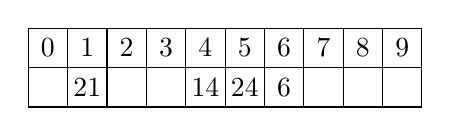
\begin{tikzpicture}[scale=0.5]
\draw (0,-1) grid (10,1);
\foreach \x in {0,1,...,9} \node at (0.5+\x,0.5) {\x};
\node at (1.5,-0.5) {$21$};
\node at (6.5,-0.5) {$6$};
\node at (4.5,-0.5) {$14$};
\node at (5.5,-0.5) {$24$};
\end{tikzpicture}
\caption{Avointa hajautusta käyttävä hajautustaulu, joka vastaa joukkoa $\{6,14,21,24\}$.
Hajautusfunktiona on $f(x)=x \bmod N$.}
\label{fig:hajavo}
\end{figure}

\begin{figure}
\center
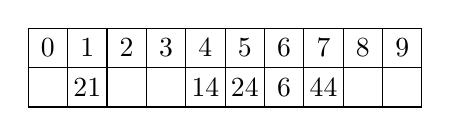
\begin{tikzpicture}[scale=0.5]
\draw (0,-1) grid (10,1);
\foreach \x in {0,1,...,9} \node at (0.5+\x,0.5) {\x};
\node at (1.5,-0.5) {$21$};
\node at (6.5,-0.5) {$6$};
\node at (4.5,-0.5) {$14$};
\node at (5.5,-0.5) {$24$};
\node at (7.5,-0.5) {$44$};
\end{tikzpicture}
\caption{Hajautustauluun lisätään vielä alkio 44, jonka hajautusarvo on 4.
Sille löytyy paikka vasta kohdasta 7.}
\label{fig:hajav2}
\end{figure}

Kun haluamme löytää alkion $x$ hajautustaulusta avointa hajautusta käyt\-täen,
tutkimme hajautustaulun kohtia kokeilufunktion mukaisesti,
kunnes joko löydämme alkion tai tulemme tyhjään kohtaan, jolloin voimme päätellä,
että hajautustaulussa ei ole alkiota.
Esimerkiksi kun haluamme löytää kuvan \ref{fig:hajav2} hajautustaulusta
alkion 44, aloitamme kohdasta $f(44)=4$ ja kuljemme eteenpäin kohtaan 7 asti.

Alkion poistaminen aiheuttaa hieman ongelmia avoimessa hajautuksessa,
koska jos vain merkitsemme alkion kohdan tyhjäksi, tämä voi häiritä tulevia hakuja.
Esimerkiksi jos poistaisimme kuvan \ref{fig:hajav2} hajautustaulusta alkion 6
merkitsemällä kohdan 6 tyhjäksi, emme enää löytäisi alkiota 44,
koska haku pysähtyisi tyhjään kohtaan 6.
Kuitenkin voimme kiertää ongelman käyttämällä jotain erikoismerkkiä
poistetulle alkiolle. Kuvassa \ref{fig:hajav3} poistetun alkion merkkinä on X,
joka tarkoittaa, että kyseinen kohta on tyhjä mutta siinä on ollut alkio.
Niinpä alkion 44 haku ei pääty tähän kohtaan,
vaikka siihen voi myös sijoittaa uuden alkion myöhemmin.

\begin{figure}
\center
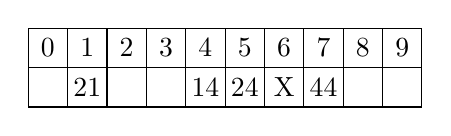
\begin{tikzpicture}[scale=0.5]
\draw (0,-1) grid (10,1);
\foreach \x in {0,1,...,9} \node at (0.5+\x,0.5) {\x};
\node at (1.5,-0.5) {$21$};
\node at (6.5,-0.5) {X};
\node at (4.5,-0.5) {$14$};
\node at (5.5,-0.5) {$24$};
\node at (7.5,-0.5) {$44$};
\end{tikzpicture}
\caption{Hajautustaulusta on poistettu alkio 6, jonka tilalla on merkki X.
Tämän ansiosta alkion 44 haku ei pysähdy kohtaan 6.}
\label{fig:hajav3}
\end{figure}

Avoimen hajautuksen tehokkuus riippuu käytetystä hajautusfunktiosta
ja kokeilufunktiosta.
Hajaustustaulun operaatiot vievät aikaa $O(m)$,
missä $m$ on kokeiltavien paikkojen määrä,
kun haluamme löytää paikan uudelle alkiolle
tai etsiä alkion taulusta.
Käytännössä lineaarisessa kokeilussa voi tulla ongelmaksi,
että alkiot kasautuvat tiettyihin hajautustaulun osiin.
Kehittyneemmissä kokeilufunktioissa alkion paikan etsimisessä
tehdään vaihtelevan kokoisia hyppyjä hajautustaulussa.

\subsection{Hajautusfunktion valinta}

Hajautusfunktio $f(x)$ määrittää, mihin kohtaan hajautustaulua
alkio $x$ sijoitetaan.
Sen täytyy antaa jokaiselle mahdolliselle alkiolle
hajautusarvo eli kokonaisluku väliltä $0,1,\dots,N-1$,
missä $N$ on hajautustaulun koko.
Kun tämä ehto täyttyy, hajautusfunktion voi muilta osin
suunnitella periaatteessa miten tahansa.
Mutta miten hajautusfunktio kannattaa valita?

Jos hajautettavat alkiot ovat kokonaislukuja,
suoraviivainen hajautusfunktio on esimerkissä käyttämämme $f(x)=x \bmod N$,
joka muuttaa luvun välille $0 \dots N-1$ jakojäännöksen avulla.
Tämä on helposti toteutettava ja yleensä hyvin toimiva hajautusfunktio.
Entä jos alkiot ovat jotain muuta tyyppiä kuin kokonaislukuja?
Tällöin voimme ensin keksiä jonkin järkevän keinon
muuttaa alkion kokonaisluvuksi,
minkä jälkeen voimme jälleen ottaa jakojäännöksen $N$:llä.

Tarkastellaan tilannetta, jossa haluamme hajauttaa merkkijonoja
eli täy\-tyy löytää tapa muuttaa merkkijono kokonaisluvuksi.
Oletamme, että merkkijonossa on $k$ merkkiä,
joiden merkkikoodit ovat $c_0,c_1,\dots,c_{k-1}$.
Esimerkiksi jos merkkijono on \texttt{testi},
merkkikoodit\footnote{Käytämme tässä merkkien ASCII-koodeja.
Javassa merkin \texttt{c} koodin saa
selville kirjoittamalla \texttt{(int)c},
ja Pythonissa voi käyttää funktiota \texttt{ord(c)}.} ovat $c_0=116$, $c_1=101$, $c_2=115$,
$c_3=116$ ja $c_4=105$.
Yksi tapa muuttaa merkkijono kokonaisluvuksi
on laskea merkkikoodien summa
\[ c_0 + c_1 + \dots + c_{k-1},\]
jolloin merkkijonoa \texttt{testi} vastaa kokonaisluku
\[116+101+115+116+105=553.\]

\index{polynominen hajautus}

Tämä on sinänsä järkevä tapa laskea hajautusarvo, mutta siinä on yksi ongelma:
kaksi merkkijonoa saavat aina saman hajautusarvon,
jos niissä on samat merkit eri järjestyksessä.
Pystymme parantamaan hajautusarvon laskentaa lisäämällä
summaan \emph{kertoimet} käyttäen kaavaa
\[ A^{k-1} c_0 + A^{k-2} c_1 + \dots + A^0 c_{k-1},\]
missä $A$ on vakio.
Esimerkiksi jos $A=7$, merkkijonoa \texttt{testi} vastaa kokonaisluku
\[7^4 \cdot 116+7^3 \cdot 101+7^2 \cdot 115+7^1 \cdot 116+7^0 \cdot 105=319711.\]
Tämän menetelmän nimi on \emph{polynominen hajautus}
(\emph{polynomial hashing}),
ja se on yksi käytännössä hyvä merkkijonon hajautustapa.

\subsection{Miten hyvin hajautus toimii?}

Hajautustaulun operaatiot vievät aikaa $O(m)$,
missä $m$ on ketjuhajautuksessa listan pituus
ja avoimessa hajautuksessa kokeilujonon pituus.
Mutta kuinka suuri $m$ on? Tähän vaikuttavat
alkioiden määrä $n$, hajautustaulun koko $N$,
hajautusfunktio $f$ sekä avoimessa hajautuksessa
kokeilufunktio $h$.

Jos kaikki sujuu hyvin, hajautusfunktio jakaa alkioita
tasaisesti hajautustaulun eri puolille
ja listojen tai kokeilujonojen pituus on luokkaa $n/N$.
Niinpä jos valitsemme hajautustaulun koon niin,
että $N$ on samaa luokkaa kuin $n$,
operaatiot toimivat tehokkaasti ajassa $O(1)$.
Kuitenkin on myös mahdollista, että hajautus epäonnistuu
ja alkiot jakautuvat hajautustauluun epätasaisesti.
Pahimmassa tapauksessa kaikki alkiot saavat saman
hajautusarvon ja ne kaikki tallennetaan samaan listaan
tai kokeilujonoon, jolloin operaatiot vievät aikaa $O(n)$.

Hajautuksessa vaikeutena on, ettemme tiedä etukäteen,
mitä alkioita hajautustauluun tallennetaan.
Tarkastellaan tilannetta,
jossa hajautettavat alkiot ovat kokonaislukuja
ja käytössä on hajautusfunktio $f(x) = x \bmod N$.
Tämä on hyvä hajautusfunktio olettaen,
että eri jakojäännöksiä esiintyy tasaisesti aineistossa.
Tämä oletus ei kuitenkaan välttämättä päde:
esimerkiksi voi olla, että jostain syystä
jokainen hajautettava alkio on parillinen.
Nyt jos myös $N$ on parillinen, jokainen hajautusarvo
on parillinen ja vain puolet hajautustaulun kohdista on käytössä.
Parempi tapa voi olla valita $N$ niin, että se on \emph{alkuluku}.
Tällöin on vähemmän todennäköistä,
että aineistossa mahdollisesti olevat säännöllisyydet
aiheuttaisivat törmäyksiä.

Emme voi kuitenkaan koskaan olla etukäteen varmoja,
että hajautus toimii hyvin.
Riippumatta hajautustavasta
\emph{ilkeä vastustaja} voi antaa
joukon alkioita, jotka kaikki saavat saman hajautusarvon.
Kaikeksi onneksi hajautus toimii yleensä aina \emph{käytännössä}
hyvin ja voimme ajatella, että hajautustaulun operaatiot ovat
$O(1)$-aikaisia, kunhan hajautustaulun koko on riittävän suuri ja
hajautus on toteutettu järke\-västi.
Vaikka on mahdollista, että hajautus epäonnistuu,
tämän riski on pieni eikä meidän tarvitse yleensä murehtia
siitä käytännössä.

\subsection{Hajautustaulu hakemistona}

\index{hakemisto}

Tähän mennessä olemme tallentaneet hajautustauluun
alkioiden joukon,
mutta voimme tallentaa myös avain-arvo-pareja,
joissa avaimen hajautusarvo määrittää,
mihin hajautustaulun kohtaan pari sijoitetaan.
Saamme näin aikaan \emph{hakemiston},
jota voi ajatella taulukon yleistyksenä.
Taulukossa avaimet ovat kokonaisluvut 0, 1, 2, jne.,
mutta hakemistossa ne voivat olla mitä tahansa arvoja
kuten merkkijonoja.

Kuvassa \ref{fig:hajhak} on esimerkkinä hajautustauluun
tallennettu hakemisto, joka vastaa seuraavaa ''taulukkoa'':

\begin{code}
taulu["abc"] = 5
taulu["xyz"] = 1
taulu["aaa"] = 8
\end{code}

Tässä tapauksessa hakemiston avaimet ovat merkkijonoja
ja arvot ovat kokonaislukuja.
Hajautustaulun ansiosta voimme käsitellä hakemistoa
taulukon tavoin niin, että operaatiot vievät aikaa $O(1)$.

\begin{figure}
\center
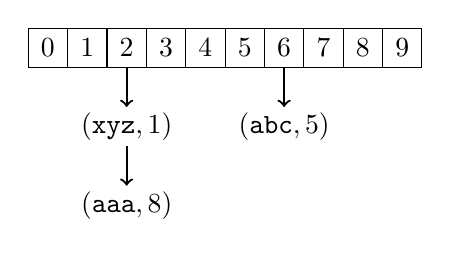
\begin{tikzpicture}[scale=0.5]
\draw (0,0) grid (10,1);
\foreach \x in {0,1,...,9} \node at (0.5+\x,0.5) {\x};
\draw[->,thick] (2.5,0) -- (2.5,-1);
\draw[->,thick] (6.5,0) -- (6.5,-1);
\draw[->,thick] (2.5,-2) -- (2.5,-3);
\node at (2.5,-3.5) {$(\texttt{aaa},8)$};
\node at (2.5,-1.5) {$(\texttt{xyz},1)$};
\node at (6.5,-1.5) {$(\texttt{abc},5)$};
\end{tikzpicture}
\caption{Hakemiston tallentaminen hajautustauluun.}
\label{fig:hajhak}
\end{figure}

Voimme myös toteuttaa hakemiston, jonka avaimet ovat kokonaislukuja.
Tällaisessa tietorakenteessa on järkeä, jos avaimet ovat niin suuria,
että emme voi käyttää hajautustaulun sijasta tavallista taulukkoa.
Kuitenkin jos avaimet ovat pieniä kokonaislukuja,
taulukko on parempi valinta, koska sen vakiokertoimet
ovat paljon hajautustaulua pienemmät.

\section{Ohjelmointikielten toteutukset}

\subsection{Java}

Javan tietorakenne \texttt{HashSet} on
hajautusta käyttävä joukko.
Esimerkiksi seuraava koodi luo joukon, johon tallennetaan
kokonaislukuja:

\begin{code}
HashSet<Integer> joukko = new HashSet<>();
joukko.add(3);
joukko.add(5);
joukko.add(8);
System.out.println(joukko.contains(5)); // true
joukko.remove(5);
System.out.println(joukko.contains(5)); // false
\end{code}

Tietorakenne \texttt{HashMap} on hajautukseen
perustuva hakemisto, joka sisäl\-tää avain-arvo-pareja.
Esimerkiksi seuraava koodi luo hakemiston,
jossa avaimet ovat merkkijonoja ja arvot ovat kokonaislukuja:

\begin{code}
HashMap<String,Integer> hakemisto = new HashMap<>();
hakemisto.put("apina",1);
hakemisto.put("banaani",2);
hakemisto.put("cembalo",3);
System.out.println(hakemisto.get("apina")); // 1
\end{code}

Java käyttää hajautuksessa ketjuhajautusta ja olettaa,
että luokissa on metodi \texttt{hashCode},
jonka avulla olio kertoo pyydettäessä hajautusarvonsa.
Metodin tulee palauttaa jokin kokonaisluku, jonka perusteella
lasketaan paikka hajautustaulussa. Seuraava koodi testaa hajautusta:

\begin{code}
System.out.println(((Integer)123).hashCode()); // 123
System.out.println("apina".hashCode()); // 93022541
\end{code}

Tästä näkee, että kokonaisluvun hajautusarvo on suoraan
kyseinen luku.
Huomaa, että meidän täytyy muuttaa luku oliotyyppiseksi
(\texttt{Integer}), jotta voimme kutsua \texttt{hashCode}-metodia.
Merkkijonon \texttt{apina} hajautusarvo on puolestaan 93022541.
On tunnettua, että Java käyttää merkkijonon hajautusarvon laskemiseen
polynomista hajautusta vakiolla $A=31$,
joten voimme laskea Javan hajautusarvon myös itse seuraavasti:
\[31^4 \cdot 97+31^3 \cdot 112+31^2 \cdot 105+31^1 \cdot 110+31^0 \cdot 97=93022541\]

\subsection{Python}

Pythonin tietorakenne \texttt{set} on hajautusta käyttävä joukko.
Seuraava koodi luo joukon ja lisää sinne kokonaislukuja:

\begin{code}
joukko = set()
joukko.add(3)
joukko.add(5)
joukko.add(8)
print(5 in joukko) # True
joukko.remove(5)
print(5 in joukko) # False
\end{code}

Tietorakenne \texttt{dict} (merkitään lyhyesti \texttt{\string{\string}})
on puolestaan hajautukseen perustuva hakemisto.
Voimme käyttää hakemistoa vaikkapa näin:

\begin{code}
hakemisto = {}
hakemisto["apina"] = 1
hakemisto["banaani"] = 2
hakemisto["cembalo"] = 3
print(hakemisto["apina"]) # 1
\end{code}

Pythonissa hajautus on toteutettu avoimella hajautuksella,
ja funktio \texttt{hash} antaa olion hajautusarvon.
Voimme testata funktion toimintaa Python-tulkissa näin:

\begin{code}
>>> hash(123)
123
>>> hash("apina")
-3191961394091913473
\end{code}

Pythonissa merkkijonon hajautusarvo lasketaan menetelmällä,
jonka toiminta vaihtelee satunnaisesti ohjelman eri suorituskerroilla.
Niinpä jos käyn\-nistämme Python-tulkin uudestaan, saamme eri tuloksen:

\begin{code}
>>> hash("apina")
-5370222958536247804
\end{code}

Tämän satunnaisuuden etuna on, että mahdollinen ilkeä vastustaja
ei voi etsiä kiinteää joukkoa merkkijonoja, jotka tuottavat saman hajautusarvon
Pythonissa, koska hajautustapa muuttuu joka suorituskerralla.

\section{Hajautustaulu algoritmeissa}

Hajautustaulun ansiosta voimme käyttää algoritmeissamme
joukkoja ja hakemistoja, joiden operaatiot toimivat tehokkaasti.
Voimme alkajaisiksi ratkoa mukavammin ajassa $O(n)$ sellaisia ongelmia,
jotka olemme ratkoneet aiemmin järjestämisen avulla ajassa $O(n \log n)$.

Aloitamme ongelmasta, jossa haluamme selvittää,
montako eri alkiota taulukko sisältää.
Ratkaisimme ongelman aiemmin
järjestämällä taulukon ja tutkimalla sen jälkeen
vierekkäisiä alkioita.
Nyt kun käytös\-sämme on hajautustaulu, voimme vain lisätä
kaikki alkiot joukkoon ja hakea lopuksi joukon koon.
Näin saamme aikaan seuraavan algoritmin:

\begin{code}
alkiot = []
for i = 0 to n-1
    alkiot.add(taulu[i])
print(alkiot.size())
\end{code}

Tässä \texttt{alkiot} on hajautustaulua käyttävä joukko,
minkä ansiosta algoritmi toimii ajassa $O(n)$.

Tarkastellaan sitten ongelmaa, jossa haluamme selvittää
taulukon yleisimmän alkion.
Ratkaisimme tämänkin ongelman aiemmin
järjestä\-mällä taulukon, mutta
hajautustaulun avulla voimme lähestyä ongelmaa
toisella tavalla luomalla hakemiston,
jonka avaimet ovat taulukon alkioita ja arvot niiden
esiintymiskertoja.
Nyt voimme vain käydä läpi taulukon sisällön ja
pitää kirjaa, montako kertaa mikäkin alkio esiintyy taulukossa:

\begin{code}
laskuri = []
suurin = 0
for i = 0 to n-1
    laskuri[taulu[i]] += 1
    if laskuri[taulu[i]] > suurin
        suurin = laskuri[taulu[i]]
        yleisin = taulu[i]
print(yleisin)
\end{code}

Tässä hakemisto \texttt{laskuri}
on toteutettu hajautustaulun avulla,
jolloin avaimet voivat olla mitä tahansa lukuja
ja operaatiot toimivat ajassa $O(1)$.
Tuloksena on algoritmi, jonka aikavaativuus on $O(n)$.

Kuten nämä esimerkit osoittavat, hajautustaulu
\emph{helpottaa} algoritmien luomista,
koska ongelmia ei tarvitse pukea järjestämisen muotoon
vaan voimme käsitellä niitä suoremmin.
Mutta toisaalta olemme ratkoneet vain uudestaan ongelmia,
jotka ovat hoituneet mainiosti myös järjestämisen avulla.
Antaisiko hajautustaulu meille jotain todellisia uusia
mahdollisuuksia algoritmien suunnittelussa?

Hajautustaulu osoittaa todelliset kyntensä silloin,
kun haluamme pitää yllä aidosti \emph{dynaamista}
tietorakennetta eli haluamme vuorotellen muuttaa
tietorakennetta ja hakea sieltä tietoa.
Tällöin emme voisi enää toteuttaa algoritmia,
joka järjestää koko aineiston kerran alussa.
Esimerkki tällaisesta tilanteesta on,
että käytössämme on funktio \texttt{hae\_luku},
joka antaa lukuja yksi kerrallaan.
Jokaisen luvun jälkeen meidän tulee ilmoittaa,
montako eri lukua olemme saaneet tähän mennessä,
ennen kuin voimme pyytää funktiolta seuraavan luvun.
Voimme ratkaista ongelman seuraavasti ajassa $O(n)$
hajautustaulun avulla:

\begin{code}
alkiot = []
for i = 1 to n
    luku = hae_luku()
    alkiot.add(luku)
    print(alkiot.size())
\end{code}

\index{online-algoritmi}
\index{offline-algoritmi}

Tällaisesta algoritmista käytetään joskus nimeä
\emph{online-algoritmi}.
Tämä tarkoittaa, että algoritmille annetaan syötettä
alkio kerrallaan ja algoritmi pystyy ilmoittamaan senhetkisen
vastauksen joka alkion käsittelyn jälkeen.
Vastaavasti \emph{offline-algoritmi} tarvitsee
käyttöönsä heti koko syötteen,
jotta se voi käsitellä syötettä kokonaisuutena,
kuten järjestää sen.
Monissa ongelmissa online-algoritmi on vaikeampi
saada aikaan kuin offline-algoritmi.

\chapter{Binäärihakupuu}

\index{binäärihakupuu}

\emph{Binäärihakupuu} (\emph{binary search tree})
on tietorakenne, joka pitää yllä
alkioiden joukkoa, samaan tapaan kuin hajautustaulu.
Binäärihakupuu eroaa hajautustaulusta kuitenkin siinä,
että se säilyttää alkioita \emph{järjestyksessä}.
Tämän ansiosta voimme esimerkiksi etsiä tehokkaasti
joukon pienimmän tai suurimman alkion,
mikä ei ole mahdollista hajautustaulussa.

Aloitamme luvun tutustumalla binääripuiden teoriaan,
minkä jälkeen perehdymme binäärihakupuun toimintaan.
Käsittelemme binäärihakupuun tehokkaasta toteutuksesta
esimerkkinä AVL-puun,
joka on yksinkertainen tasapainoinen binäärihakupuu.
Tasapainotuksen ansiosta saamme toteutettua binäärihakupuun niin,
että sen operaatiot ovat tehokkaita.

\section{Taustaa binääripuista}

\index{binääripuu}

Binäärihakupuun taustalla on yleisempi tietorakenne \emph{binääripuu}
(\emph{binary tree}).
Ennen kuin tutustumme binäärihakupuuhun,
onkin hyvä selvittää ensin, mikä on binääripuu ja mitä
ominaisuuksia siihen liittyy.

\index{juuri}
\index{lapsi}
\index{vanhempi}
\index{lehti}

Binääripuu muodostuu $n$ solmusta.
Puussa ylimpänä on solmu, jota kutsutaan \emph{juureksi} (\emph{root}).
Jokaisella solmulla voi olla vasen ja oikea \emph{lapsi} (\emph{child}),
ja kaikilla solmuilla juurta lukuun ottamatta on yksikäsitteinen
\emph{vanhempi} (\emph{parent}).
Puun \emph{lehtiä} (\emph{leaf}) ovat solmut, joilla ei ole lapsia.

\index{alipuu}

Binääripuun rakenne on rekursiivinen:
jokainen solmu toimii juurena \emph{alipuulle} (\emph{subtree}),
joka on myös binääripuu.
Solmun $x$ alipuu sisältää solmun $x$ sekä kaikki
solmut, joihin pääsee laskeutumalla alaspäin solmusta $x$.
Voimme myös ajatella asiaa niin, että jokaisen binääripuun
solmun vasen ja oikea lapsi on toinen (mahdollisesti tyhjä) binääripuu.

\begin{figure}
\center
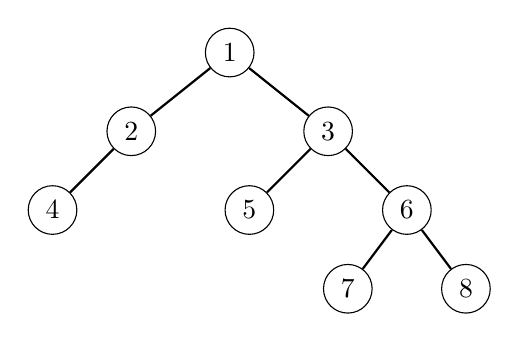
\begin{tikzpicture}[scale=0.5]
\node[draw, circle] (1) at (0,0) {$1$};
\node[draw, circle] (2) at (-2.5,-2) {$2$};
\node[draw, circle] (3) at (2.5,-2) {$3$};
\node[draw, circle] (4) at (-4.5,-4) {$4$};
\node[draw, circle] (5) at (0.5,-4) {$5$};
\node[draw, circle] (6) at (4.5,-4) {$6$};
\node[draw, circle] (7) at (3,-6) {$7$};
\node[draw, circle] (8) at (6,-6) {$8$};
\path[draw,thick,-] (1) -- (2);
\path[draw,thick,-] (1) -- (3);
\path[draw,thick,-] (2) -- (4);
\path[draw,thick,-] (3) -- (5);
\path[draw,thick,-] (3) -- (6);
\path[draw,thick,-] (6) -- (7);
\path[draw,thick,-] (6) -- (8);
\end{tikzpicture}
\caption{Binääripuu, jossa on 8 solmua. Puun juuri on solmu 1,
ja puun lehtiä ovat solmut 4, 5, 7 ja 8.}
\label{fig:binpuu}
\end{figure}

Kuvassa \ref{fig:binpuu} on esimerkki binääripuusta, jossa on 8 solmua.
Solmu 1 on puun juuri, ja solmut 4, 5, 7 ja 8 ovat puun lehtiä.
Solmun 3 vasen lapsi on solmu 5, oikea lapsi on solmu 6
ja vanhempi on solmu 1.
Solmun 3 alipuu sisältää solmut 3, 5, 6, 7 ja 8.

Binääripuun juuren \emph{syvyys} (\emph{depth}) on 0 ja jokaisen muun solmun syvyys on yhtä
suurempi kuin sen vanhemman syvyys.
Binääripuun \emph{korkeus} (\emph{height}) on puolestaan
suurin puun solmussa esiintyvä syvyys
eli toisin sanoen suurin askelten määrä juuresta alaspäin lehteen.
Esimerkiksi kuvan \ref{fig:binpuu} puun korkeus on 3,
koska solmujen 7 ja 8 syvyys on 3.

\begin{figure}
\center
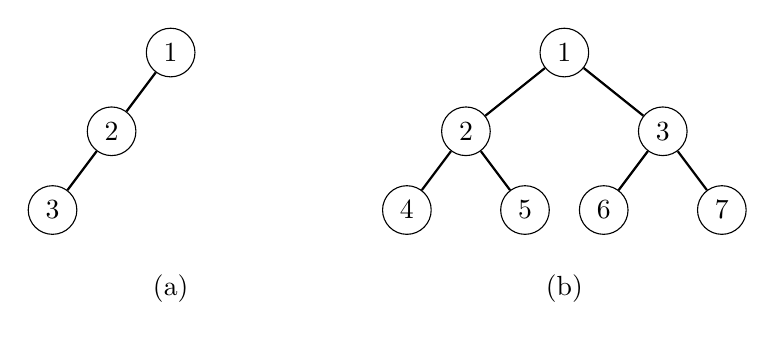
\begin{tikzpicture}[scale=0.5]
\begin{scope}
\node[draw, circle] (1) at (0,0) {$1$};
\node[draw, circle] (2) at (-1.5,-2) {$2$};
\node[draw, circle] (3) at (-3,-4) {$3$};
\path[draw,thick,-] (1) -- (2);
\path[draw,thick,-] (2) -- (3);
\node at (0,-6) {(a)};
\end{scope}
\begin{scope}[xshift=10cm]
\node[draw, circle] (1) at (0,0) {$1$};
\node[draw, circle] (2) at (-2.5,-2) {$2$};
\node[draw, circle] (3) at (2.5,-2) {$3$};
\node[draw, circle] (4) at (-4,-4) {$4$};
\node[draw, circle] (5) at (-1,-4) {$5$};
\node[draw, circle] (6) at (1,-4) {$6$};
\node[draw, circle] (7) at (4,-4) {$7$};
\path[draw,thick,-] (1) -- (2);
\path[draw,thick,-] (1) -- (3);
\path[draw,thick,-] (2) -- (4);
\path[draw,thick,-] (2) -- (5);
\path[draw,thick,-] (3) -- (6);
\path[draw,thick,-] (3) -- (7);
\node at (0,-6) {(b)};
\end{scope}
\end{tikzpicture}
\caption{(a) Vähiten solmuja sisältävä korkeuden 2 binääripuu.
(b) Eniten solmuja sisältävä korkeuden 2 binääripuu.}
\label{fig:binraj}
\end{figure}

Jos binääripuun korkeus on $h$, siinä on vähintään $h+1$ solmua,
jolloin puu on pelkkä solmujen lista,
ja enintään $2^{h+1}-1$ solmua,
jolloin kaikilla tasoilla on kaikki mahdolliset solmut.
Kuva \ref{fig:binraj} näyttää esimerkit näistä tapauksista,
kun puun korkeus on $2$.

\subsection{Binääripuun käsittely}

Voimme toteuttaa binääripuun linkitettynä rakenteena niin,
että jokainen puun solmu on olio, jossa on viittaus
vasempaan ja oikeaan lapseen sekä mahdollisesti
muita kenttiä, kuten solmuun liittyvä arvo.
Jos solmulla ei ole vasenta tai oikeaa lasta,
viittauksena on \texttt{null}.

Rekursio on luonteva tapa toteuttaa monia
binääripuun käsittelyyn liittyviä operaatioita.
Esimerkiksi seuraava funktio laskee, montako solmua
sille annetussa puussa on:

\begin{code}
function laske_solmut(solmu)
    if solmu == null
        return 0
    return 1 + laske_solmut(solmu.vasen) +
                laske_solmut(solmu.oikea)
\end{code}

Funktiolle annetaan parametrina solmu,
joka vastaa puun juurta.
Jos puu on tyhjä, siinä ei ole yhtään solmua.
Muuten puussa on juurisolmu sekä vasemman
ja oikean alipuun solmut.
Pystymme laskemaan alipuiden solmut rekursiivisesti
kutsumalla samaa funktiota uudestaan.

Seuraava funktio puolestaan selvittää, mikä on puun korkeus.
Huomaa, että jos puu on tyhjä, tulkintana on,
että sen korkeus on $-1$.

\begin{code}
function korkeus(solmu)
    if solmu == null
        return -1
    return 1 + max(korkeus(solmu.vasen), korkeus(solmu.oikea))
\end{code}

\subsection{Läpikäyntijärjestykset}

Voimme käydä läpi binääripuun solmut rekursiivisesti
juuresta alkaen.
Solmujen läpikäyntiin on kolme tavallista järjestystä:

\index{esijärjestys}
\index{sisäjärjestys}
\index{jälkijärjestys}

\begin{itemize}
\item \emph{esijärjestys} (\emph{pre-order}): käsittelemme ensin juuren, sitten vasemman alipuun
ja lopuksi oikean alipuun
\item \emph{sisäjärjestys} (\emph{in-order}): käsittelemme ensin vasemman alipuun, sitten juuren
ja lopuksi oikean alipuun
\item \emph{jälkijärjestys} (\emph{post-order}): käsittelemme ensin vasemman alipuun,
sitten oikean alipuun ja lopuksi juuren
\end{itemize}

Esimerkiksi kuvan \ref{fig:binpuu} puussa
esijärjestys on $[1,2,4,3,5,6,7,8]$,
sisäjärjes\-tys on $[4,2,1,5,3,7,6,8]$ ja
jälkijärjestys on $[4,2,5,7,8,6,3,1]$.

Voimme käydä binääripuun solmut läpi kaikissa yllä mainituissa
järjes\-tyksissä rekursion avulla.
Esimerkiksi seuraava proseduuri tulostaa puun solmut
sisäjärjestyksessä, kun sille annetaan parametrina
puun juuri:

\begin{code}
procedure lapikaynti(solmu)
    if solmu == null
        return
    lapikaynti(solmu.vasen)
    print(solmu.arvo)
    lapikaynti(solmu.oikea)
\end{code}

\section{Binäärihakupuun toiminta}

Binäärihakupuu on binääripuu, jonka kukin solmu
vastaa yhtä joukon alkiota.
Solmut on järjestetty niin, että jokaisessa solmussa
kaikki vasemman alipuun solmut ovat arvoltaan pienempiä
ja vastaavasti kaikki oikean alipuun solmut
ovat arvoltaan suurempia.
Tämän ansiosta voimme löytää kätevästi halutun
alkion puusta aloittamalla haun puun juuresta.

\begin{figure}
\center
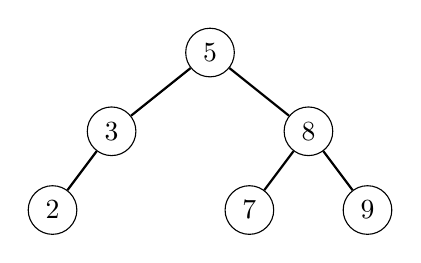
\begin{tikzpicture}[scale=0.5]
\node[draw, circle] (1) at (0,0) {$5$};
\node[draw, circle] (2) at (-2.5,-2) {$3$};
\node[draw, circle] (3) at (2.5,-2) {$8$};
\node[draw, circle] (4) at (-4,-4) {$2$};
\node[draw, circle] (5) at (1,-4) {$7$};
\node[draw, circle] (6) at (4,-4) {$9$};
\path[draw,thick,-] (1) -- (2);
\path[draw,thick,-] (1) -- (3);
\path[draw,thick,-] (2) -- (4);
\path[draw,thick,-] (3) -- (5);
\path[draw,thick,-] (3) -- (6);
\end{tikzpicture}
\caption{Joukkoa $\{2,3,5,7,8,9\}$ vastaava binäärihakupuu.}
\label{fig:bihpuu}
\end{figure}

Kuvassa \ref{fig:bihpuu} on esimerkkinä
joukkoa $\{2,3,5,7,8,9\}$ vastaava binääri\-hakupuu,
jonka juurena on alkio 5.
Vasemmassa alipuussa on kaikki alkiota 5
pienemmät alkiot, eli se vastaa joukkoa $\{2,3\}$.
Oikeassa alipuussa taas on kaikki alkiota 5
suuremmat alkiot, eli se vastaa joukkoa $\{7,8,9\}$.
Huomaa, että tämä on yksi monista tavoista muodostaa
binäärihakupuu kyseiselle joukolle ja voisimme valita myös
minkä tahansa muun alkion puun juureksi.

\subsection{Operaatioiden toteutus}

Seuraavaksi käymme läpi, kuinka voimme toteuttaa
binäärihakupuun avulla operaatioita joukon alkioiden käsittelemiseen.
Osoittautuu, että voimme toteuttaa kaikki
operaatiot ajassa $O(h)$, missä $h$ on puun korkeus.

\subsubsection{Alkion etsiminen}

Kun haluamme etsiä joukosta alkiota $x$, lähdemme liikkeelle
puun juuresta ja kuljemme alaspäin puussa.
Kun olemme solmussa, jossa on alkio $a$,
vaihtoehtoja on kolme.
Jos $a=x$, olemme löytäneet halutun alkion,
jos $a>x$, jatkamme hakua solmun vasempaan lapseen,
ja jos $a<x$, jatkamme hakua solmun oikeaan lapseen.
Jos kuitenkaan solmulla ei ole lasta,
johon meidän tulisi edetä, toteamme,
ettei joukossa ole alkiota $x$.

\begin{figure}
\center
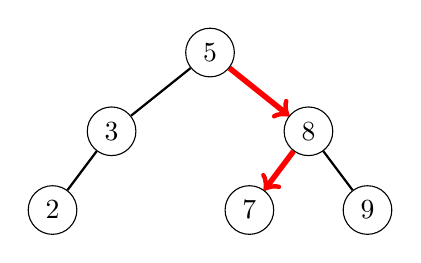
\begin{tikzpicture}[scale=0.5]
\node[draw, circle] (1) at (0,0) {$5$};
\node[draw, circle] (2) at (-2.5,-2) {$3$};
\node[draw, circle] (3) at (2.5,-2) {$8$};
\node[draw, circle] (4) at (-4,-4) {$2$};
\node[draw, circle] (5) at (1,-4) {$7$};
\node[draw, circle] (6) at (4,-4) {$9$};
\path[draw,thick,-] (1) -- (2);
\path[draw,thick,-] (1) -- (3);
\path[draw,thick,-] (2) -- (4);
\path[draw,thick,-] (3) -- (5);
\path[draw,thick,-] (3) -- (6);
\path[draw,thick,red,line width=2pt,->] (1) -- (3);
\path[draw,thick,red,line width=2pt,->] (3) -- (5);
\end{tikzpicture}
\caption{Alkion $7$ etsiminen joukosta $\{2,3,5,7,8,9\}$ juuresta alkaen.}
\label{fig:bihets}
\end{figure}

Kuva \ref{fig:bihets} näyttää, kuinka löydämme alkion 7
joukosta $\{2,3,5,7,8,9\}$.
Juurena on alkio 5, joten alkion 7 täytyy olla juuren
oikeassa alipuussa.
Tämän alipuun juurena on alkio 8,
joten nyt taas tiedämme, että alkion 7 täytyy olla
vasemmassa alipuussa, josta se löytyykin.

\subsubsection{Alkion lisääminen}

Kun haluamme lisätä joukkoon alkion $x$,
jota ei vielä ole joukossa, kuljemme ensin
puussa aivan kuin etsisimme alkiota $x$.
Sitten kun olemme päässeet solmuun,
jolla ei ole lasta, johon meidän tulisi edetä,
luomme uuden solmun alkiolle $x$ ja lisäämme
sen tähän kohtaan lapseksi.

\begin{figure}
\center
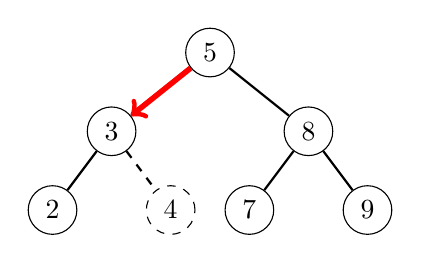
\begin{tikzpicture}[scale=0.5]
\node[draw, circle] (1) at (0,0) {$5$};
\node[draw, circle] (2) at (-2.5,-2) {$3$};
\node[draw, circle] (3) at (2.5,-2) {$8$};
\node[draw, circle] (4) at (-4,-4) {$2$};
\node[draw, circle] (5) at (1,-4) {$7$};
\node[draw, circle] (6) at (4,-4) {$9$};
\node[draw, circle, dashed] (7) at (-1,-4) {$4$};
\path[draw,thick,-] (1) -- (2);
\path[draw,thick,-] (1) -- (3);
\path[draw,thick,-] (2) -- (4);
\path[draw,thick,-] (3) -- (5);
\path[draw,thick,-] (3) -- (6);
\path[draw,thick,dashed,-] (2) -- (7);
\path[draw,thick,red,line width=2pt,->] (1) -- (2);
\end{tikzpicture}
\caption{Alkion 4 lisääminen joukkoon $\{2,3,5,7,8,9\}$.}
\label{fig:bihpu2}
\end{figure}

Kuva \ref{fig:bihpu2} näyttää, kuinka lisäämme alkion 4
joukkoon $\{2,3,5,7,8,9\}$.
Kun haemme puusta alkiota 4, päädymme solmuun,
jossa on alkio 3 ja jolla ei ole oikeaa lasta.
Niinpä luomme alkiolle 4 uuden solmun, jonka asetamme
alkion 3 solmun oikeaksi lapseksi.

\subsubsection{Pienin alkio / suurin alkio}

Kun haluamme löytää joukon pienimmän alkion,
lähdemme liikkeelle juuresta ja etenemme joka askeleella
solmun vasempaan lapseen.
Kun solmulla ei ole enää vasenta lasta,
olemme löytäneet joukon pienimmän alkion.

Vastaavalla tavalla löydämme joukon suurimman alkion
etenemällä koko ajan oikeaan lapseen juuresta.

\subsubsection{Seuraava suurempi alkio / edellinen pienempi alkio}

Kun haluamme löytää joukon pienimmän alkion,
joka on suurempi kuin $x$,
lähdemme liikkeelle puun juuresta.
Kun olemme solmussa, jossa on alkio $a$,
etenemme vasempaan lapseen,
jos $a>x$, ja oikeaan lapseen, jos $a \le x$.
Jatkamme näin, kunnes emme voi edetä alemmas.
Haluttu alkio on pienin alkiota $x$ suurempi alkio
kaikista alkioista, joiden kautta kuljimme.

Kun haluamme vastaavasti löytää joukon suurimman alkion,
joka on pienempi kuin $x$,
menettelemme käänteisesti edelliseen nähden.

\subsubsection{Alkion poistaminen}

Kun haluamme poistaa joukosta alkion $x$, etsimme ensin
alkiota $x$ vastaavan solmun tavalliseen tapaan.
Jos solmulla ei ole lapsia tai vain yksi lapsi,
on helppoa poistaa solmu puusta ja säilyttää
puun rakenne muuten ennallaan.
Jos kuitenkin solmulla on kaksi lasta,
tilanne on hankalampi.
Tällöin etsimme alkion $y$,
joka on pienin $x$:ää suurempi alkio,
ja vaihdamme keskenään alkiot $x$ ja $y$ puussa.
Tämän jälkeen on helppoa poistaa solmu,
jossa on nyt alkio $x$,
koska sillä ei voi olla kahta lasta
(jos solmulla olisi vasen lapsi,
$y$ ei olisi pienin $x$:ää suurempi alkio).

\begin{figure}
\center
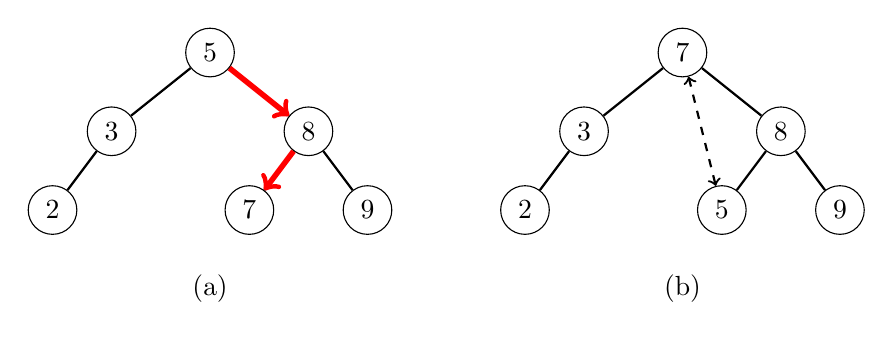
\begin{tikzpicture}[scale=0.5]
\begin{scope}
\node[draw, circle] (1) at (0,0) {$5$};
\node[draw, circle] (2) at (-2.5,-2) {$3$};
\node[draw, circle] (3) at (2.5,-2) {$8$};
\node[draw, circle] (4) at (-4,-4) {$2$};
\node[draw, circle] (5) at (1,-4) {$7$};
\node[draw, circle] (6) at (4,-4) {$9$};
\path[draw,thick,-] (1) -- (2);
\path[draw,thick,-] (1) -- (3);
\path[draw,thick,-] (2) -- (4);
\path[draw,thick,-] (3) -- (5);
\path[draw,thick,-] (3) -- (6);
\path[draw,thick,red,line width=2pt,->] (1) -- (3);
\path[draw,thick,red,line width=2pt,->] (3) -- (5);
\node at (0,-6) {(a)};
\end{scope}
\begin{scope}[xshift=12cm]
\node[draw, circle] (1) at (0,0) {$7$};
\node[draw, circle] (2) at (-2.5,-2) {$3$};
\node[draw, circle] (3) at (2.5,-2) {$8$};
\node[draw, circle] (4) at (-4,-4) {$2$};
\node[draw, circle] (5) at (1,-4) {$5$};
\node[draw, circle] (6) at (4,-4) {$9$};
\path[draw,thick,-] (1) -- (2);
\path[draw,thick,-] (1) -- (3);
\path[draw,thick,-] (2) -- (4);
\path[draw,thick,-] (3) -- (5);
\path[draw,thick,-] (3) -- (6);
\path[draw,thick,<->,dashed] (1) -- (5);
\node at (0,-6) {(b)};
\end{scope}
\end{tikzpicture}
\caption{Alkion 5 poistaminen joukosta $\{2,3,5,7,8,9\}$. (a) Koska alkiolla
5 on kaksi lasta, etsimme seuraavan suuremman alkion 7.
(b) Vaihdamme keskenään alkiot 5 ja 7, minkä jälkeen voimme poistaa helposti alkion 5.}
\label{fig:bihpu3}
\end{figure}

Kuva \ref{fig:bihpu3} näyttää, kuinka poistamme joukosta $\{2,3,5,7,8,9\}$ alkion 5.
Alkio on puun juuressa ja solmulla on kaksi lasta,
joten meidän tulee etsiä ensin pienin alkiota 5 suurempi alkio,
joka on 7.
Vaihdamme sitten keskenään arvot 5 ja 7,
minkä jälkeen on helppoa poistaa alkio 5.

\subsection{Operaatioiden tehokkuus}

Binäärihakupuun operaatiot vievät aikaa $O(h)$,
missä $h$ on puun korkeus, joten operaatioiden tehokkuus
riippuu puun korkeudesta.
Operaatioiden tehokkuuteen vaikuttaa siis,
miten olemme rakentaneet puun.
Esimerkiksi kuvassa \ref{fig:bihkor} on kaksi mahdollista
binäärihakupuuta joukolle $\{1,2,3,4,5\}$.
Vasemman puun korkeus on 2, kun taas oikean puun korkeus on 4.

\begin{figure}
\center
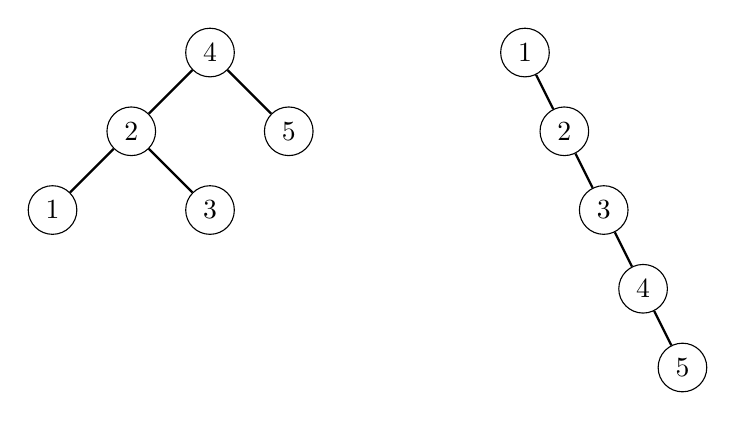
\begin{tikzpicture}[scale=0.5]
\begin{scope}
\node[draw, circle] (1) at (0,0) {$1$};
\node[draw, circle] (2) at (1,-2) {$2$};
\node[draw, circle] (3) at (2,-4) {$3$};
\node[draw, circle] (4) at (3,-6) {$4$};
\node[draw, circle] (5) at (4,-8) {$5$};
\path[draw,thick,-] (1) -- (2);
\path[draw,thick,-] (2) -- (3);
\path[draw,thick,-] (3) -- (4);
\path[draw,thick,-] (4) -- (5);
\end{scope}
\begin{scope}[xshift=-8cm]
\node[draw, circle] (1) at (0,0) {$4$};
\node[draw, circle] (2) at (-2,-2) {$2$};
\node[draw, circle] (3) at (2,-2) {$5$};
\node[draw, circle] (4) at (-4,-4) {$1$};
\node[draw, circle] (5) at (0,-4) {$3$};
\path[draw,thick,-] (1) -- (2);
\path[draw,thick,-] (1) -- (3);
\path[draw,thick,-] (2) -- (4);
\path[draw,thick,-] (2) -- (5);
\end{scope}
\end{tikzpicture}
\caption{Kaksi binäärihakupuuta joukolle $\{1,2,3,4,5\}$.
Vasemman puun korkeus on 2 ja oikean puun korkeus on 4.}
\label{fig:bihkor}
\end{figure}

\index{tasapainoinen puu}

Jotta binäärihakupuu toimisi tehokkaasti, haluamme,
että puun korkeus ei kasva liian suureksi.
Tarkemmin ottaen tavoitteena on, että
solmut ovat jakautuneet tasaisesti puun eri puolille
ja puun korkeus on $O(\log n)$
eli puu on \emph{tasapainoinen} (\emph{balanced}).
Jos onnistumme tässä, kaikki puun operaatiot toimivat
tehokkaasti ajassa $O(\log n)$.
Saavutamme tavoitteen
lisäämällä puuhun ehtoja, jotka rajoittavat
sen korkeutta sopivasti.

Binäärihakupuun tasapainottamiseen tunnetaan monia menetelmiä.
Tutustumme seuraavaksi AVL-puuhun, joka on 
varhaisin tunnettu tasapainoinen binäärihakupuu.
AVL-puu on yksinkertaisempi kuin monet myöhemmin
kehitetyt rakenteet, minkä vuoksi se sopii hyvin esittelemään
puiden tasapainotuksen ideoita.
Ohjelmointikielten standardikirjastoissa
käytetään kuitenkin yleensä muita rakenteita kuten punamustaa puuta.

\section{AVL-puu}

\index{AVL-puu}

\emph{AVL-puu} (\emph{AVL tree}) on tasapainoinen binäärihakupuu, jonka
korkeus on aina $O(\log n)$, minkä ansiosta puun operaatiot
toimivat tehokkaasti ajassa $O(\log n)$.
AVL-puussa jokaiseen solmuun liittyy \emph{tasapainoehto},
joka takaa, että puu on tasapainoinen.
Puuta päivittäessä täytyy pitää huolta siitä,
että tasapainoehto säilyy voimassa kaikissa solmuissa.

\subsection{Tasapainoehto}

AVL-puun tasapainoehtona on, että
\emph{jokaisessa solmussa vasemman ja oikean lapsen
alipuiden korkeusero on enintään 1}.

Esimerkiksi kuvan \ref{fig:bihkor} vasen puu on
AVL-puu, kun taas oikea puu ei ole.
Oikea puu ei ole AVL-puu, koska esimerkiksi solmussa 1
vasemman lapsen alipuun korkeus on $-1$ mutta oikean lapsen
alipuun korkeus on 3.
Korkeuksien erona on siis 4, vaikka ero saisi olla enintään 1.

\index{AVL-ehto}

Kutsumme AVL-puun tasapainoehtoa \emph{AVL-ehdoksi}.
Osoittautuu, että jos binäärihakupuu täyttää AVL-ehdon,
sen korkeus on $O(\log n)$.
Eli jos pystymme toteuttamaan puun operaatiot niin,
että AVL-ehto säilyy, saamme aikaan binäärihakupuun,
jonka operaatiot toimivat ajassa $O(\log n)$.

\begin{figure}
\center
\scriptsize
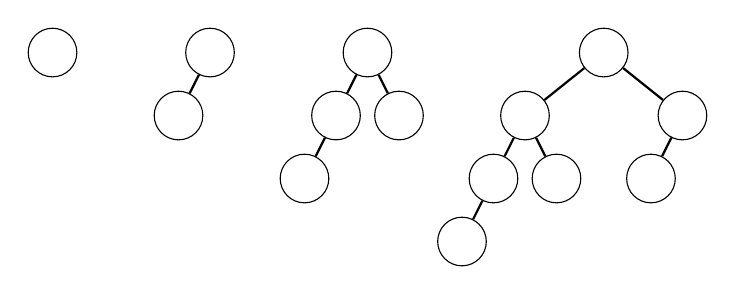
\begin{tikzpicture}[scale=0.4]
\begin{scope}
\node[draw, circle] (2) at (-2.5,-2) {\phantom{$1$}};
\end{scope}
\begin{scope}[xshift=5cm]
\node[draw, circle] (2) at (-2.5,-2) {\phantom{$1$}};
\node[draw, circle] (4) at (-3.5,-4) {\phantom{$1$}};
\path[draw,thick,-] (2) -- (4);
\end{scope}
\begin{scope}[xshift=10cm]
\node[draw, circle] (2) at (-2.5,-2) {\phantom{$1$}};
\node[draw, circle] (4) at (-3.5,-4) {\phantom{$1$}};
\node[draw, circle] (5) at (-1.5,-4) {\phantom{$1$}};
\node[draw, circle] (7) at (-4.5,-6) {\phantom{$1$}};
\path[draw,thick,-] (2) -- (4);
\path[draw,thick,-] (2) -- (5);
\path[draw,thick,-] (4) -- (7);
\end{scope}
\begin{scope}[xshift=15cm,yshift=-2cm]
\node[draw, circle] (1) at (0,0) {\phantom{$1$}};
\node[draw, circle] (2) at (-2.5,-2) {\phantom{$1$}};
\node[draw, circle] (3) at (2.5,-2) {\phantom{$1$}};
\node[draw, circle] (4) at (-3.5,-4) {\phantom{$1$}};
\node[draw, circle] (5) at (-1.5,-4) {\phantom{$1$}};
\node[draw, circle] (6) at (1.5,-4) {\phantom{$1$}};
\node[draw, circle] (7) at (-4.5,-6) {\phantom{$1$}};
\path[draw,thick,-] (1) -- (2);
\path[draw,thick,-] (1) -- (3);
\path[draw,thick,-] (2) -- (4);
\path[draw,thick,-] (2) -- (5);
\path[draw,thick,-] (3) -- (6);
\path[draw,thick,-] (4) -- (7);
\end{scope}
\end{tikzpicture}
\caption{Vähiten solmuja sisältävät AVL-puut korkeuksille 0, 1, 2 ja 3.}
\label{fig:avlvah}
\end{figure}

Miksi sitten AVL-ehto takaa, että binäärihakupuun korkeus
on $O(\log n)$?
Voimme lähestyä asiaa pahimman tapauksen kautta:
kun tiedämme, että AVL-puussa on $n$ solmua,
mikä on sen \emph{suurin mahdollinen} korkeus?
Voimme selvittää tämän laskemalla ensin käänteisesti,
mikä on \emph{pienin mahdollinen} solmujen määrä
AVL-puussa, jonka korkeus on $h$.

Merkitään $f(h)$:lla korkeutta $h$ olevan AVL-puun
pienintä mahdollista solmujen määrää.
Kuvan \ref{fig:avlvah} mukaisesti funktion ensimmäiset arvot
ovat $f(0)=1$, $f(1)=2$, $f(2)=4$ ja $f(3)=7$.
Yleisemmin
\[f(h)=1+f(h-1)+f(h-2),\]
kun $h \ge 2$, koska jos haluamme rakentaa AVL-puun korkeutta $h$,
jossa on mahdollisimman vähän solmuja,
meidän kannattaa laittaa juuren lapsiksi AVL-puut
korkeutta $h-1$ ja $h-2$ niin,
että kummassakin alipuussa on mahdollisimman vähän solmuja.
Funktiolle pätee
\[f(h) \ge 2 f(h-2),\]
eli funktion arvo ainakin kaksinkertaistuu kahden askeleen välein.
Voimme ilmaista tämän alarajan
\[f(h) \ge 2^{h/2},\]
jonka voimme taas muuttaa ylärajaksi
\[ h \le 2 \log f(h).\]

Tarkastellaan sitten puuta, jossa on $n$ solmua
ja jonka korkeus on $h$.
Korkeudelle täytyy päteä $f(h) \le n$,
koska korkeutta $h$ olevassa puussa on vähintään $f(h)$ solmua.
Niinpä saamme ylärajan
\[h \le 2 \log n,\]
mikä tarkoittaa samaa kuin $h = O(\log n)$.

\subsection{Kiertojen toteuttaminen}

\begin{figure}
\center
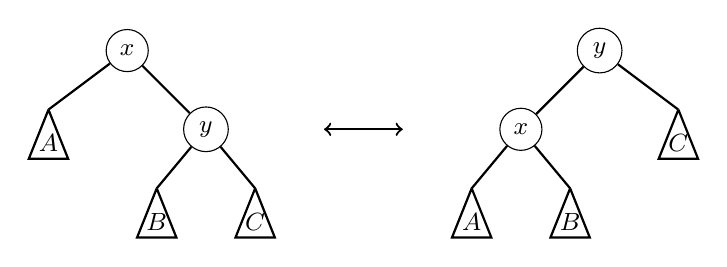
\begin{tikzpicture}[scale=0.5]
\small
\newcommand\alipuu[3]{
\path[draw,thick,-] (0+#1,0+#2) -- (-0.5+#1,-1.25+#2) -- (0.5+#1,-1.25+#2) -- (0+#1,0+#2);
\node at (0+#1,-0.85+#2) {#3};
}
\draw[thick,<->] (5,-2) -- (7,-2);
\begin{scope}
\node[draw, circle] (1) at (0,0) {$x$};
\node[draw, circle] (2) at (2,-2) {$y$};
\alipuu{-2}{-1.5}{$A$}
\alipuu{0.75}{-3.5}{$B$}
\alipuu{3.25}{-3.5}{$C$}
\path[draw,thick,-] (1) -- (2);
\path[draw,thick,-] (1) -- (-2,-1.5);
\path[draw,thick,-] (2) -- (0.75,-3.5);
\path[draw,thick,-] (2) -- (3.25,-3.5);
\end{scope}
\begin{scope}[xshift=10cm]
\node[draw, circle] (1) at (0,-2) {$x$};
\node[draw, circle] (2) at (2,0) {$y$};
\alipuu{-1.25}{-3.5}{$A$}
\alipuu{1.25}{-3.5}{$B$}
\alipuu{4}{-1.5}{$C$}
\path[draw,thick,-] (1) -- (2);
\path[draw,thick,-] (1) -- (-1.25,-3.5);
\path[draw,thick,-] (1) -- (1.25,-3.5);
\path[draw,thick,-] (2) -- (4,-1.5);
\end{scope}
\end{tikzpicture}
\caption{Kierrot, joiden avulla korjaamme AVL-puuta.}
\label{fig:avlkie}
\end{figure}

\index{kierto}

Voimme toteuttaa AVL-puun operaatiot muuten samaan tapaan
kuin yleisessä binäärihakupuussa, mutta 
alkion lisäämisen ja poistamisen jälkeen täy\-tyy varmistaa,
että AVL-ehto on edelleen voimassa.
Tämä onnistuu tekemällä sopivia \emph{kiertoja} (\emph{rotation}),
jotka muuttavat puun rakennetta.
Jotta voimme toteuttaa kierrot, pidämme jokaisessa
solmussa tietoa siitä, mikä on solmusta alkavan alipuun korkeus.

Osoittautuu, että voimme korjata puun rakenteen kaikissa
tilanteessa käyttäen kahta kiertotyyppiä,
jotka on esitetty kuvassa \ref{fig:avlkie}.
Kierrämme solmuja $x$ ja $y$,
joihin liittyvät alipuut $A$, $B$ ja $C$.
Voimme tehdä kierron joko vasemmalta oikealle,
jolloin solmu $y$ nousee ylöspäin,
tai oikealta vasemmalle,
jolloin solmu $x$ nousee ylöspäin.

\begin{figure}
\center
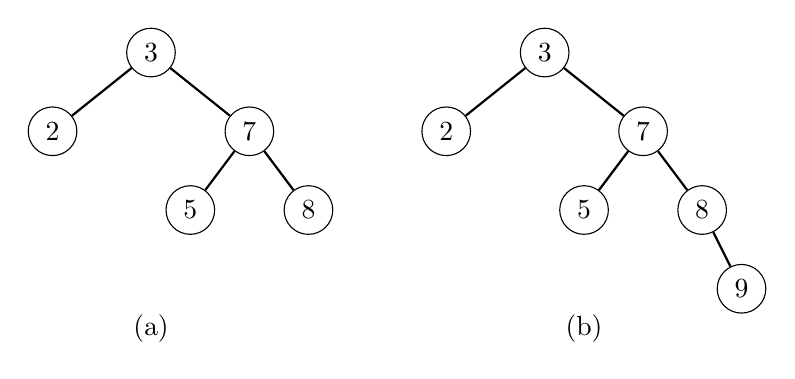
\begin{tikzpicture}[scale=0.5]
\begin{scope}
\node[draw, circle] (1) at (0,0) {$3$};
\node[draw, circle] (2) at (-2.5,-2) {$2$};
\node[draw, circle] (3) at (2.5,-2) {$7$};
\node[draw, circle] (5) at (1,-4) {$5$};
\node[draw, circle] (6) at (4,-4) {$8$};
\path[draw,thick,-] (1) -- (2);
\path[draw,thick,-] (1) -- (3);
\path[draw,thick,-] (3) -- (5);
\path[draw,thick,-] (3) -- (6);
\node at (0,-7) {(a)};
\end{scope}
\begin{scope}[xshift=10cm]
\node[draw, circle] (1) at (0,0) {$3$};
\node[draw, circle] (2) at (-2.5,-2) {$2$};
\node[draw, circle] (3) at (2.5,-2) {$7$};
\node[draw, circle] (5) at (1,-4) {$5$};
\node[draw, circle] (6) at (4,-4) {$8$};
\node[draw, circle] (7) at (5,-6) {$9$};
\path[draw,thick,-] (1) -- (2);
\path[draw,thick,-] (1) -- (3);
\path[draw,thick,-] (3) -- (5);
\path[draw,thick,-] (3) -- (6);
\path[draw,thick,-] (6) -- (7);
\node at (1,-7) {(b)};
\end{scope}
\end{tikzpicture}
\caption{(a) Jokaisessa puun solmussa pätee AVL-ehto.
(b) AVL-ehto menee rikki solmussa 3, kun lisäämme puuhun solmun 9.}
\label{fig:avlrik}
\end{figure}

Kun lisäämme AVL-puuhun solmun, jonkin solmun AVL-ehto
voi rikkoontua. Tämä ilmenee niin,
että jossain solmussa lasten alipuiden korkeudet ovat ennen lisäämistä
$h$ ja $h+1$ ja lisäämisen jälkeen $h$ ja $h+2$.
Kuva \ref{fig:avlrik} näyttää esimerkin tällaisesta tilanteesta.
Vasemmassa puussa solmun $3$ lasten korkeudet ovat 0 ja 1,
joten AVL-ehto on kunnossa.
Oikeassa puussa olemme lisänneet solmun $9$,
minkä seurauksena solmun $3$ lasten korkeudet ovat 0 ja 2
eikä AVL-ehto enää päde.

\begin{figure}
\center
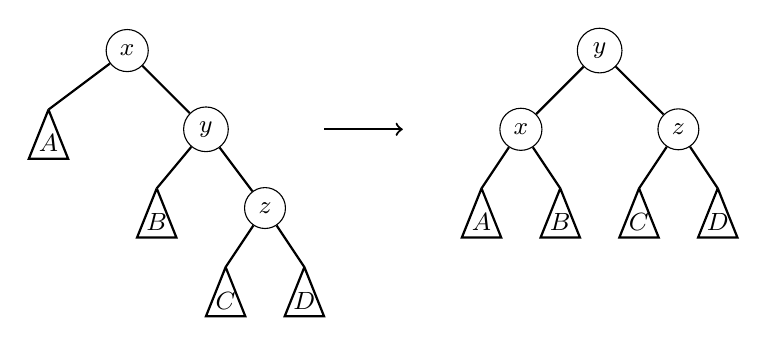
\begin{tikzpicture}[scale=0.5]
\small
\newcommand\alipuu[3]{
\path[draw,thick,-] (0+#1,0+#2) -- (-0.5+#1,-1.25+#2) -- (0.5+#1,-1.25+#2) -- (0+#1,0+#2);
\node at (0+#1,-0.85+#2) {#3};
}
\draw[thick,->] (5,-2) -- (7,-2);
\begin{scope}
\node[draw, circle] (1) at (0,0) {$x$};
\node[draw, circle] (2) at (2,-2) {$y$};
\node[draw, circle] (3) at (3.5,-4) {$z$};
\alipuu{-2}{-1.5}{$A$}
\alipuu{0.75}{-3.5}{$B$}
\alipuu{2.5}{-5.5}{$C$}
\alipuu{4.5}{-5.5}{$D$}
\path[draw,thick,-] (1) -- (2);
\path[draw,thick,-] (2) -- (3);
\path[draw,thick,-] (1) -- (-2,-1.5);
\path[draw,thick,-] (2) -- (0.75,-3.5);
\path[draw,thick,-] (3) -- (2.5,-5.5);
\path[draw,thick,-] (3) -- (4.5,-5.5);
\end{scope}
\begin{scope}[xshift=12cm]
\node[draw, circle] (1) at (-2,-2) {$x$};
\node[draw, circle] (2) at (0,0) {$y$};
\node[draw, circle] (3) at (2,-2) {$z$};
\alipuu{-3}{-3.5}{$A$}
\alipuu{-1}{-3.5}{$B$}
\alipuu{1}{-3.5}{$C$}
\alipuu{3}{-3.5}{$D$}
\path[draw,thick,-] (1) -- (2);
\path[draw,thick,-] (2) -- (3);
\path[draw,thick,-] (1) -- (-3,-3.5);
\path[draw,thick,-] (1) -- (-1,-3.5);
\path[draw,thick,-] (3) -- (1,-3.5);
\path[draw,thick,-] (3) -- (3,-3.5);
\end{scope}
\end{tikzpicture}
\caption{Tapaus 1: nostamme solmua $y$ ylöspäin.}
\label{fig:avlta1}
\end{figure}

\begin{figure}
\center
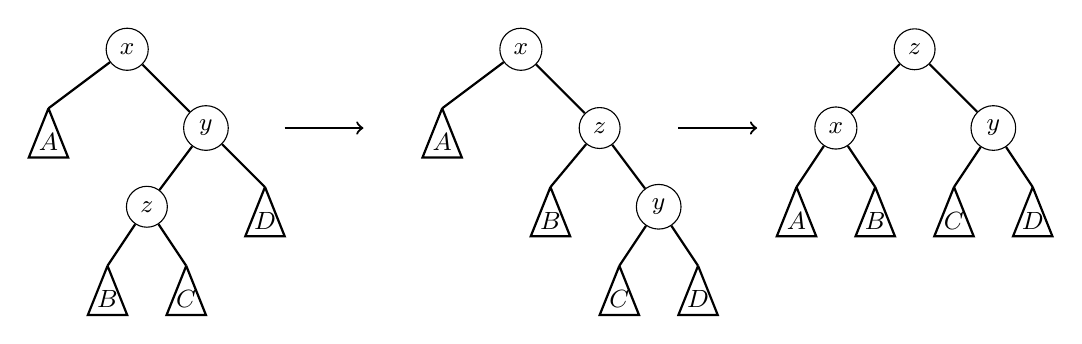
\begin{tikzpicture}[scale=0.5]
\small
\newcommand\alipuu[3]{
\path[draw,thick,-] (0+#1,0+#2) -- (-0.5+#1,-1.25+#2) -- (0.5+#1,-1.25+#2) -- (0+#1,0+#2);
\node at (0+#1,-0.85+#2) {#3};
}
\draw[thick,->] (4,-2) -- (6,-2);
\draw[thick,->] (14,-2) -- (16,-2);
\begin{scope}
\node[draw, circle] (1) at (0,0) {$x$};
\node[draw, circle] (2) at (2,-2) {$y$};
\node[draw, circle] (3) at (0.5,-4) {$z$};
\alipuu{-2}{-1.5}{$A$}
\alipuu{-0.5}{-5.5}{$B$}
\alipuu{1.5}{-5.5}{$C$}
\alipuu{3.5}{-3.5}{$D$}
\path[draw,thick,-] (1) -- (2);
\path[draw,thick,-] (2) -- (3);
\path[draw,thick,-] (1) -- (-2,-1.5);
\path[draw,thick,-] (3) -- (-0.5,-5.5);
\path[draw,thick,-] (3) -- (1.5,-5.5);
\path[draw,thick,-] (2) -- (3.5,-3.5);
\end{scope}
\begin{scope}[xshift=10cm]
\node[draw, circle] (1) at (0,0) {$x$};
\node[draw, circle] (2) at (2,-2) {$z$};
\node[draw, circle] (3) at (3.5,-4) {$y$};
\alipuu{-2}{-1.5}{$A$}
\alipuu{0.75}{-3.5}{$B$}
\alipuu{2.5}{-5.5}{$C$}
\alipuu{4.5}{-5.5}{$D$}
\path[draw,thick,-] (1) -- (2);
\path[draw,thick,-] (2) -- (3);
\path[draw,thick,-] (1) -- (-2,-1.5);
\path[draw,thick,-] (2) -- (0.75,-3.5);
\path[draw,thick,-] (3) -- (2.5,-5.5);
\path[draw,thick,-] (3) -- (4.5,-5.5);
\end{scope}
\begin{scope}[xshift=20cm]
\node[draw, circle] (1) at (-2,-2) {$x$};
\node[draw, circle] (2) at (0,0) {$z$};
\node[draw, circle] (3) at (2,-2) {$y$};
\alipuu{-3}{-3.5}{$A$}
\alipuu{-1}{-3.5}{$B$}
\alipuu{1}{-3.5}{$C$}
\alipuu{3}{-3.5}{$D$}
\path[draw,thick,-] (1) -- (2);
\path[draw,thick,-] (2) -- (3);
\path[draw,thick,-] (1) -- (-3,-3.5);
\path[draw,thick,-] (1) -- (-1,-3.5);
\path[draw,thick,-] (3) -- (1,-3.5);
\path[draw,thick,-] (3) -- (3,-3.5);
\end{scope}
\end{tikzpicture}
\caption{Tapaus 2: nostamme solmua $z$ kahdesti ylöspäin.}
\label{fig:avlta2}
\end{figure}

Solmun lisäämisen jälkeen kuljemme puussa ylöspäin
lisätystä solmusta juureen ja päivitämme solmujen korkeudet.
Jos jokin solmu ei täytä AVL-ehtoa, korjaamme asian tekemällä yhden
tai kaksi kiertoa.
Oletetaan, että $x$ on alimpana puussa oleva solmu, jossa AVL-ehto ei päde,
$y$ on $x$:n lapsi, jonka alipuussa on lisätty solmu,
ja $z$ on puolestaan $y$:n lapsi, jonka alipuussa on lisätty solmu.
Tapauksia on kaksi: jos $y$ ja $z$ ovat samanpuoleisia lapsia,
kierrämme solmua $y$ kerran ylöspäin (kuva \ref{fig:avlta1}),
ja muuten kierrämme solmua $z$ kahdesti ylöspäin (kuva \ref{fig:avlta2}).
Tämän korjauksen jälkeen AVL-ehto on jälleen
voimassa kaikissa puun solmuissa, eli riittää aina
korjata ehto alimmassa solmussa, jossa se ei ole voimassa.

Kuvassa \ref{fig:avlrik}(b) AVL-ehto ei ole voimassa solmussa $3$,
koska vasemman alipuun korkeus on 0 ja oikean alipuun korkeus on 2.
Tässä tapauksessa $x=3$, $y=7$ ja $z=8$.
Koska $y$ on $x$:n oikea lapsi ja $z$ on $y$:n oikea lapsi,
meidän riittää tehdä yksi kierto, joka nostaa solmua $7$ ylöspäin
puun juureksi.
Tuloksena on kuvan \ref{fig:avlkor} mukainen puu, jossa
AVL-ehto on jälleen voimassa,
koska solmun $7$ kummankin alipuun korkeus on nyt 1.

\begin{figure}
\center
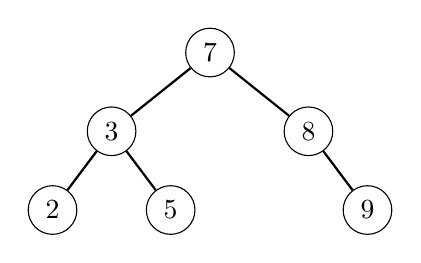
\begin{tikzpicture}[scale=0.5]
\node[draw, circle] (1) at (0,0) {$7$};
\node[draw, circle] (2) at (-2.5,-2) {$3$};
\node[draw, circle] (3) at (2.5,-2) {$8$};
\node[draw, circle] (5) at (-4,-4) {$2$};
\node[draw, circle] (6) at (-1,-4) {$5$};
\node[draw, circle] (7) at (4,-4) {$9$};
\path[draw,thick,-] (1) -- (2);
\path[draw,thick,-] (1) -- (3);
\path[draw,thick,-] (2) -- (5);
\path[draw,thick,-] (2) -- (6);
\path[draw,thick,-] (3) -- (7);
\end{tikzpicture}
\caption{Kierrämme solmun $7$ puun juureksi, jolloin AVL-ehto pätee taas.}
\label{fig:avlkor}
\end{figure}

Kun poistamme puusta solmun, menettelemme melko samalla tavalla
kuin lisäämisessä.
Nyt on mahdollista, että ennen poistoa
jossakin solmussa lasten alipuiden korkeudet ovat $h$ ja $h-1$
ja poiston jälkeen $h$ ja $h-2$.
Poiston jälkeen nousemme puussa ylöspäin
poistetun solmun vanhemmasta alkaen, ja jos vastaan tulee solmu $x$,
jossa AVL-ehto ei päde, korjaamme asian.
Tällä kertaa valitsemme solmut $y$ ja $z$ niin,
että $y$ on $x$:n lapsi, jonka korkeus on suurin,
ja samoin $z$ on $y$:n lapsi, jonka korkeus on suurin.
Jos $y$:n kummankin lapsen korkeus on sama,
valitsemme $z$:n niin, että se on samanpuoleinen lapsi kuin $y$.
Sitten korjaamme AVL-ehdon kierroilla kuten solmun lisäämisessä.
Toisin kuin lisäämisessä, saatamme joutua korjaamaan ehdon
useassa solmussa,
koska ehdon korjaaminen yhdessä solmussa voi rikkoa
sen jossain ylemmässä solmussa.
Kun lopulta saavumme juureen, AVL-ehto pätee jälleen kaikissa solmuissa.

Koska AVL-puun korkeus on $O(\log n)$ ja jokainen kierto
tapahtuu vakioajassa,
pystymme korjaamaan tasapainon sekä lisäämisen että poistamisen
jälkeen ajassa $O(\log n)$.
Lisäämisen jälkeen kuljemme puuta ylöspäin $O(\log n)$ askelta
ja teemme enintään kaksi kiertoa.
Poistamisen jälkeen taas kuljemme puuta ylöspäin $O(\log n)$ askelta
ja teemme enintään $O(\log n)$ kiertoa.

\section{Ohjelmointikielten toteutukset}

\subsection{Java}

Javan tietorakenteet \texttt{TreeSet} ja \texttt{TreeMap}
toteuttavat tasapainoisen binääri\-hakupuun.
Ne perustuvat punamustaan puuhun, joka on AVL-puun tapainen
puurakenne mutta monimutkaisempi.
Nämä rakenteet tarjoavat samat metodit kuin
\texttt{HashSet} ja \texttt{HashMap},
mutta lisäksi tehokkaita metodeita,
jotka liittyvät alkioiden järjestykseen puussa.

Seuraava koodi luo \texttt{TreeSet}-rakenteen
ja lisää siihen lukuja:

\begin{code}
TreeSet<Integer> luvut= new TreeSet<>();
luvut.add(4);
luvut.add(1);
luvut.add(8);
luvut.add(7);
\end{code}

Koska joukko on järjestyksessä, pystymme etsimään tehokkaasti
pienim\-män ja suurimman alkion metodeilla \texttt{first} ja \texttt{last}:

\begin{code}
int pienin = joukko.first(); // 1
int suurin = joukko.last(); // 8
\end{code}

Pystymme myös etsimään tehokkaasti seuraavan tiettyä alkiota
suuremman tai pienemmän alkion metodeilla \texttt{higher} ja \texttt{lower}:

\begin{code}
int suurempi = joukko.higher(5); // 7
int pienempi = joukko.lower(5); // 4
\end{code}

Seuraava koodi luo sanakirjan \texttt{TreeMap}-rakenteen avulla:

\begin{code}
TreeMap<String,String> sanakirja = new TreeMap<>();
sanakirja.put("apina","monkey");
sanakirja.put("banaani","banana");
sanakirja.put("cembalo","harpsichord");
\end{code}

Tämä sanakirja muodostuu avain-arvo-pareista,
joissa avaimet ovat suomen kielen sanoja
ja arvot ovat englannin kielen sanoja.
Sanakirjan sisältö on järjestetty avainten perusteella.
Esimerkiksi voimme selvittää, mikä on aakkosjärjestyksessä
ensimmäinen ja viimeinen avain:

\begin{code}
String eka = sanakirja.firstKey(); // apina
String vika = sanakirja.lastKey(); // cembalo
\end{code}

Samoin voimme selvittää lähinnä tiettyä avainta olevat avaimet:

\begin{code}
String seuraava = sanakirja.higherKey("biisoni"); // cembalo
String edellinen = sanakirja.lowerKey("biisoni"); // banaani
\end{code}

\subsection{Python}

Pythonin standardikirjastossa \emph{ei} ole 
tasapainoisen binäärihakupuun toteutusta.
Tämä on kielen suunnittelussa tehty päätös,
joka liittyy ihanteeseen, että kielessä on yksi selkeä
tapa toteuttaa tietty asia.
Koska Pythonissa on hajautustaulua
käyttävät tietorakenteet \texttt{set} ja \texttt{dict},
binäärihakupuulle ei ole nähty tarvetta.

Miten selviämme Pythonissa ilman binäärihakupuuta?
Mahdollisia ratkaisuja ovat:

\begin{itemize}
\item Useissa tilanteissa hajautustaulu riittää:
binäärihakupuuta tarvitaan vain, jos haluamme etsiä
alkioita järjestyksen perusteella.
\item Vaikka järjestykselle olisi tarvetta, voimme käyttää
usein binäärihaku\-puun sijasta listan järjestämistä tai
seuraavassa luvussa käsiteltävää binäärikekoa, jonka toteutus
on Pythonin standardikirjastossa.
\item Voimme tarvittaessa käyttää myös jotain standardikirjaston
ulkopuolista binäärihakupuun toteutusta.
\end{itemize}

Itse asiassa yleinen suuntaus suosituissa ohjelmointikielissä vaikuttaa olevan,
että standardikirjastossa on tarjolla hajautustaulu mutta ei
binääri\-hakupuuta. Näin on myös JavaScript-kielessä,
jossa tietorakenteet \texttt{Set} ja \texttt{Map} käyttävät hajautustaulua.
Vaikuttaa siltä, että käytännön ohjelmoinnissa ei ole usein tarvetta säilyttää
joukon alkioita järjestyksessä.

Miksi sitten kahdesta vaihtoehtoisesta tietorakenteesta
(hajautustaulu ja binäärihakupuu) on valittu hajautustaulu,
jossa on vähemmän ominaisuuksia?
Syynä on, että hajautustaulun toteutus on paljon yksinkertaisempi,
minkä seurauksena se toimii yleensä tehokkaammin.
Ero näkyy myös aikavaativuuksissa: hajautustaulun operaatiot vievät
keskimäärin aikaa $O(1)$, kun taas binäärihakupuussa aikaa kuluu $O(\log n)$.

\section{Tehokkuusvertailu}

Monissa ongelmissa on kaksi mahdollista lähestymistapaa:
voimme käyttää joko joukkorakenteita tai taulukon järjestämistä.
Vaikka molemmat tavat johtavat tehokkaaseen ratkaisuun,
vakiokertoimissa voi olla merkittäviä eroja, jotka vaikuttavat
käytännön tehokkuuteen.

Tarkastelemme seuraavaksi ongelmaa, jossa meille on annettu
$n$ lukua sisältävä taulukko, ja haluamme selvittää,
montako eri lukua taulukossa on.
Ratkaisemme ongelman Javalla kolmella eri tavalla ja tutkimme sitten
ratkaisujen tehokkuutta.

\subsubsection{Ratkaisu 1: \texttt{TreeSet}}

Ensimmäinen tapa ratkaista tehtävä on luoda \texttt{TreeSet},
johon lisäämme taulukon luvut.
Koska jokainen luku voi esiintyä joukossa vain kerran,
joukon koko ilmaisee meille, montako eri lukua taulukossa on.
Tämä ratkaisu vie aikaa $O(n \log n)$, koska jokainen
\texttt{add}-operaatio vie aikaa $O(\log n)$.

\subsubsection{Ratkaisu 2: \texttt{HashSet}}

Emme tarvitse \texttt{TreeSet}-rakenteen
alkioiden järjestystä, joten saamme toisen ratkaisun
käyttämällä sen sijaan \texttt{HashSet}-rakennetta.
Koodi säilyy muuten täysin samanlaisena.
Tämä ratkaisu vie aikaa $O(n)$ hajautuksen ansiosta.

\subsubsection{Ratkaisu 3: järjestäminen}

Kolmas tapa ratkaista tehtävä on käyttää järjestämistä:
kopioimme ensin luvut uuteen taulukkoon, järjestämme tämän taulukon ja
tutkimme sitten, monessako kohdassa järjestetyssä taulukossa luku vaihtuu.
Tämä ratkaisu vie aikaa $O(n \log n)$, koska taulukon järjestäminen
vie aikaa $O(n \log n)$.

\subsubsection{Vertailun tulokset}

Taulukko \ref{tab:eriver} esittää tehokkuusvertailun tulokset.
Jokaisessa testissä taulukossa on satunnaisia lukuja väliltä $1 \dots 10^9$.

Osoittautuu, että ratkaisujen välillä on merkittäviä tehokkuuseroja.
Ensinnäkin \texttt{HashSet}-ratkaisu on noin kolme kertaa
nopeampi kuin \texttt{TreeSet}-ratkaisu.
Tämä onkin odotettavaa, koska hajautustaulun
operaatiot vievät aikaa $O(1)$, kun taas binäärihakupuun
operaatiot vievät aikaa $O(\log n)$.
Selvästi nopein ratkaisu on kuitenkin kolmas järjestämistä
käyttävä ratkaisu, joka on noin kymmenen kertaa
\texttt{TreeSet}-ratkaisua nopeampi.

Miten on mahdollista, että sekä \texttt{TreeSet}-ratkaisun että
järjestämisrat\-kaisun aikavaativuus on $O(n \log n)$, mutta
järjestämisratkaisu on kymmenen kertaa nopeampi?
Tämä johtuu siitä, että taulukon järjestäminen on hyvin kevyt
operaatio ja se tehdään vain kerran.
Kun sitten käytetään \texttt{TreeSet}-rakennetta,
sen taustalla joudutaan ylläpitämään tasapainoista binääri\-hakupuuta.
Tällöin alkioiden lisäykset ovat raskaita operaatioita,
koska jokaiselle uudelle alkiolle täytyy etsiä paikka puusta ja mahdollisesti
korjata lisäyksen jälkeen puun rakennetta kiertojen avulla.

Vaikka hajautustaulu ja binäärihakupuu ovat käteviä,
niitä ei siis kannata käyttää turhaan.
Jos haluamme ratkaista ongelman todella tehokkaasti,
kannattaa miettiä, voisimmeko käyttää tavalla tai toisella
järjestämistä näiden tietorakenteiden sijaan.

\begin{table}
\center
\begin{tabular}{rrrr}
taulukon koko $n$ & \texttt{TreeSet} & \texttt{HashSet} & järjestäminen \\
\hline
$10^6$ & 0.74 s & 0.25 s & 0.09 s \\
$2 \cdot 10^6$ & 1.60 s & 0.45 s & 0.19 s \\
$4 \cdot 10^6$ & 5.60 s & 1.56 s & 0.52 s \\
$8 \cdot 10^6$ & 12.19 s & 4.50 s & 0.97 s \\
\end{tabular}
\caption{Algoritmien suoritusaikojen vertailu.}
\label{tab:eriver}
\end{table}

\chapter{Keko}

\index{keko}
\index{prioriteettijono}

\emph{Keko} (\emph{heap}) on tietorakenne, jonka operaatiot ovat
alkion lisääminen sekä
pienimmän tai suurimman alkion etsiminen ja poistaminen.
Vaikka voisimme toteuttaa nämä operaatiot myös
binäärihakupuun avulla, keon etuna on, että saamme aikaan
yleistä joukkorakennetta \emph{kevyemmän} rakenteen, kun
rajoitumme tilanteeseen, jossa käytössämme on vain nämä operaatiot.

Tutustumme tässä luvussa binäärikeko-rakenteeseen,
joka on tavallisimmin käytetty kekorakenne.
Binäärikeko toteutetaan binääripuuna,
ja se mahdollistaa alkion etsimisen ajassa $O(1)$ sekä
alkioiden lisäykset ja poistot ajassa $O(\log n)$.
Pystymme toteuttamaan binäärikeon tehokkaasti taulukkona,
koska sen toiminnot ovat yleistä binääripuuta rajatumpia.

\section{Binäärikeko}

\index{binäärikeko}

\emph{Binäärikeko} (\emph{binary heap}) on binääripuu, jonka kaikki tasot
alinta tasoa lukuun ottamatta ovat täynnä solmuja.
Alimman tason solmut on puolestaan sijoitettu
mahdollisimman vasemmalle ylempien solmujen lapsiksi.

\index{minimikeko}
\index{maksimikeko}
\index{kekoehto}

Kun luomme keon, meidän täytyy päättää,
onko se \emph{minimikeko} vai \emph{maksimikeko}.
Minimikeossa voimme etsiä ja poistaa pienimmän alkion,
kun taas maksimikeossa voimme etsiä ja poistaa suurimman alkion.
Keon toiminta perustuu siihen, että jokainen
keon solmu täyttää \emph{kekoehdon}.
Minimikeossa ehtona on, että jokaisen solmun arvo on
pienempi tai yhtä suuri kuin sen kummankin lapsen arvo.
Maksimikeossa puolestaan ehtona on, että jokaisen solmun arvo
on suurempi tai yhtä suuri kuin sen kummankin lapsen arvo.
Kekoehdon ansiosta minimikeon juuressa on keon
pienin alkio ja maksimikeon juuressa on keon suurin alkio.

\begin{figure}
\center
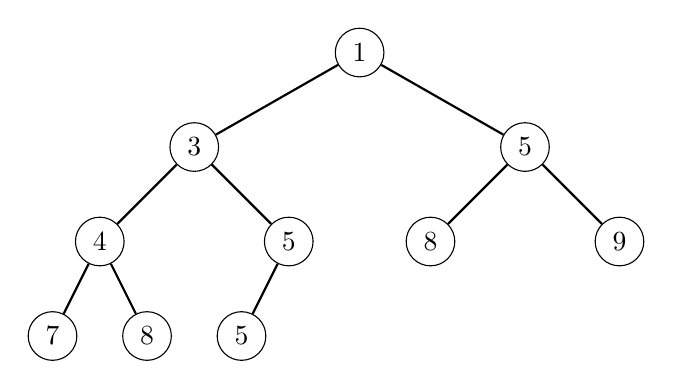
\begin{tikzpicture}[scale=0.6]
\node[draw, circle] (1) at (0,0) {$1$};
\node[draw, circle] (2) at (-3.5,-2) {$3$};
\node[draw, circle] (3) at (3.5,-2) {$5$};
\node[draw, circle] (4) at (-5.5,-4) {$4$};
\node[draw, circle] (5) at (-1.5,-4) {$5$};
\node[draw, circle] (6) at (1.5,-4) {$8$};
\node[draw, circle] (7) at (5.5,-4) {$9$};
\node[draw, circle] (8) at (-6.5,-6) {$7$};
\node[draw, circle] (9) at (-4.5,-6) {$8$};
\node[draw, circle] (10) at (-2.5,-6) {$5$};
\path[draw,thick,-] (1) -- (2);
\path[draw,thick,-] (1) -- (3);
\path[draw,thick,-] (2) -- (4);
\path[draw,thick,-] (2) -- (5);
\path[draw,thick,-] (3) -- (6);
\path[draw,thick,-] (3) -- (7);
\path[draw,thick,-] (4) -- (8);
\path[draw,thick,-] (4) -- (9);
\path[draw,thick,-] (5) -- (10);
\end{tikzpicture}
\caption{Minimikeko, joka sisältää alkiot $[1,3,4,5,5,5,7,8,8,9]$.}
\label{fig:minkek}
\end{figure}

Kuvassa \ref{fig:minkek} on minimikeko,
johon on tallennettu kymmenen alkiota.
Keon kolme ensimmäistä tasoa ovat täynnä
ja neljännellä tasolla kolme ensimmäistä kohtaa on käytetty.
Keon juurena on joukon pienin alkio $1$,
ja kaikki solmut täyttävät kekoehdon.
Huomaa, että sama alkio voi esiintyä monta kertaa keossa,
kuten tässä keossa alkiot $5$ ja $8$.

\subsection{Keon tallentaminen}

Tallennamme binäärikeon \emph{taulukkona},
joka sisältää keon solmujen arvot jär\-jestyksessä
ylhäältä alaspäin ja vasemmalta oikealle.
Tämä tehokas tallennustapa on mahdollinen,
koska keon kaikki tasot ovat täynnä solmuja.
Tavallinen tapa on tallentaa keko taulukkoon niin,
että indeksointi alkaa 1:stä.
Esimerkiksi kuvan \ref{fig:minkek} keko vastaa seuraavaa taulukkoa:
\vspace{5px}

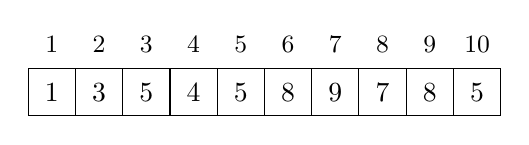
\begin{tikzpicture}[scale=0.6]
\draw (0,0) grid (10,1);
\foreach \x in {1,...,10} \node at (-0.5+\x,1.5) {\small \x};
\foreach \x/\v in {1/1,2/3,3/5,4/4,5/5,6/8,7/9,8/7,9/8,10/5} \node at (-0.5+\x,0.5) {\v};
\end{tikzpicture}

\vspace{5px}
Taulukkototeutuksen etuna on, että voimme laskea
helposti, missä kohdissa keon alkiot ovat taulukossa.
Ensinnäkin keon juuri eli pienin tai suurin alkio
on aina kohdassa $1$.
Lisäksi jos tiedämme, että tietty solmu on kohdassa $k$,
niin solmun vasen lapsi on kohdassa $2k$,
solmun oikea lapsi on kohdassa $2k+1$ ja
solmun vanhempi on kohdassa $\lfloor k/2 \rfloor$.
Esimerkissämme solmu $3$
on taulukossa kohdassa $2$,
joten sen vasen lapsi on kohdassa $4$,
oikea lapsi on kohdassa $5$ ja
vanhempi on kohdassa $1$.

Käytännössä haluamme yleensä,
että pystymme lisäämään kekoon uusia alkioita,
jolloin saattaa olla tarpeen suurentaa taulukkoa.
Voimme toteuttaa tämän samalla tavalla kuin taulukkolistassa,
jolloin taulukon suurentaminen ei hidasta keon operaatioita.

\subsection{Operaatioiden toteutus}

On helppoa etsiä minimikeon pienin alkio
tai maksimikeon suurin alkio $O(1)$-ajassa,
koska tämä alkio on aina keon juuressa.
Seuraavaksi näemme, kuinka voimme toteuttaa alkion lisäämisen
sekä pienimmän tai suurimman alkion poistamisen $O(\log n)$-ajassa.

\subsubsection{Alkion lisääminen}

Kun lisäämme uuden alkion kekoon, lisäämme sen ensin seuraavaan
vapaana olevaan paikkaan puussa. Jos alimmalla tasolla on tilaa,
lisäämme sen sinne mahdollisimman vasemmalle,
ja muuten aloitamme uuden tason, jossa on toistaiseksi vain lisättävä solmu.
Alkion lisäämisen jälkeen meidän täytyy varmistaa,
että kekoehto säilyy edelleen voimassa.
Tämä tapahtuu siirtämällä alkiota ylöspäin keossa,
kunnes kekoehto tulee voimaan.

\begin{figure}
\center
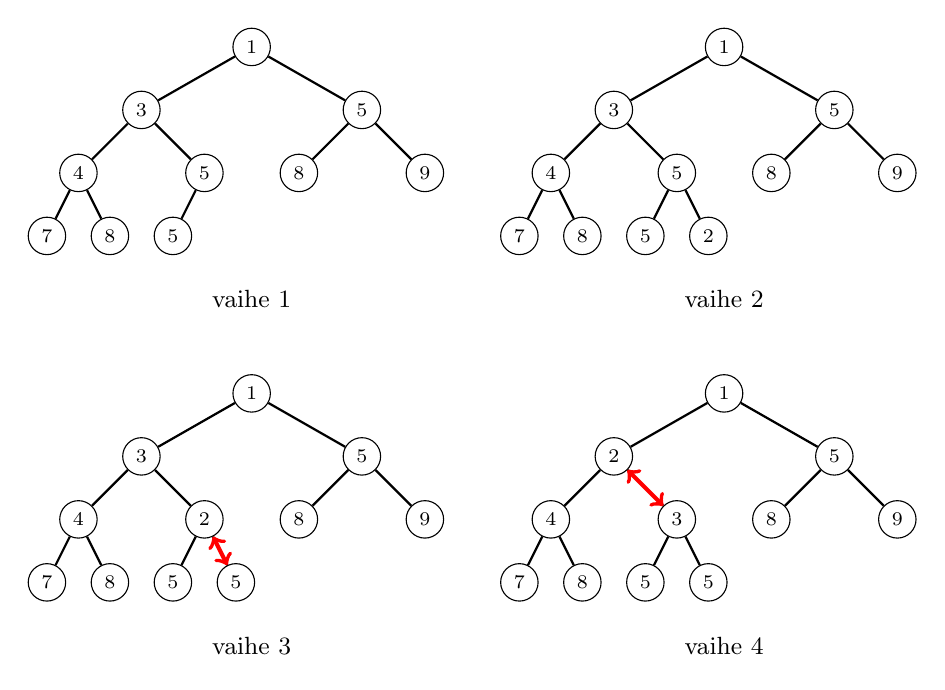
\begin{tikzpicture}[scale=0.4]
\scriptsize
\begin{scope}
\node[draw, circle] (1) at (0,0) {$1$};
\node[draw, circle] (2) at (-3.5,-2) {$3$};
\node[draw, circle] (3) at (3.5,-2) {$5$};
\node[draw, circle] (4) at (-5.5,-4) {$4$};
\node[draw, circle] (5) at (-1.5,-4) {$5$};
\node[draw, circle] (6) at (1.5,-4) {$8$};
\node[draw, circle] (7) at (5.5,-4) {$9$};
\node[draw, circle] (8) at (-6.5,-6) {$7$};
\node[draw, circle] (9) at (-4.5,-6) {$8$};
\node[draw, circle] (10) at (-2.5,-6) {$5$};
\path[draw,thick,-] (1) -- (2);
\path[draw,thick,-] (1) -- (3);
\path[draw,thick,-] (2) -- (4);
\path[draw,thick,-] (2) -- (5);
\path[draw,thick,-] (3) -- (6);
\path[draw,thick,-] (3) -- (7);
\path[draw,thick,-] (4) -- (8);
\path[draw,thick,-] (4) -- (9);
\path[draw,thick,-] (5) -- (10);
\node at (0,-8) {\small vaihe $1$};
\end{scope}
\begin{scope}[xshift=15cm]
\node[draw, circle] (1) at (0,0) {$1$};
\node[draw, circle] (2) at (-3.5,-2) {$3$};
\node[draw, circle] (3) at (3.5,-2) {$5$};
\node[draw, circle] (4) at (-5.5,-4) {$4$};
\node[draw, circle] (5) at (-1.5,-4) {$5$};
\node[draw, circle] (6) at (1.5,-4) {$8$};
\node[draw, circle] (7) at (5.5,-4) {$9$};
\node[draw, circle] (8) at (-6.5,-6) {$7$};
\node[draw, circle] (9) at (-4.5,-6) {$8$};
\node[draw, circle] (10) at (-2.5,-6) {$5$};
\node[draw, circle] (11) at (-0.5,-6) {$2$};
\path[draw,thick,-] (1) -- (2);
\path[draw,thick,-] (1) -- (3);
\path[draw,thick,-] (2) -- (4);
\path[draw,thick,-] (2) -- (5);
\path[draw,thick,-] (3) -- (6);
\path[draw,thick,-] (3) -- (7);
\path[draw,thick,-] (4) -- (8);
\path[draw,thick,-] (4) -- (9);
\path[draw,thick,-] (5) -- (10);
\path[draw,thick,-] (5) -- (11);
\node at (0,-8) {\small vaihe $2$};
\end{scope}
\begin{scope}[yshift=-11cm]
\node[draw, circle] (1) at (0,0) {$1$};
\node[draw, circle] (2) at (-3.5,-2) {$3$};
\node[draw, circle] (3) at (3.5,-2) {$5$};
\node[draw, circle] (4) at (-5.5,-4) {$4$};
\node[draw, circle] (5) at (-1.5,-4) {$2$};
\node[draw, circle] (6) at (1.5,-4) {$8$};
\node[draw, circle] (7) at (5.5,-4) {$9$};
\node[draw, circle] (8) at (-6.5,-6) {$7$};
\node[draw, circle] (9) at (-4.5,-6) {$8$};
\node[draw, circle] (10) at (-2.5,-6) {$5$};
\node[draw, circle] (11) at (-0.5,-6) {$5$};
\path[draw,thick,-] (1) -- (2);
\path[draw,thick,-] (1) -- (3);
\path[draw,thick,-] (2) -- (4);
\path[draw,thick,-] (2) -- (5);
\path[draw,thick,-] (3) -- (6);
\path[draw,thick,-] (3) -- (7);
\path[draw,thick,-] (4) -- (8);
\path[draw,thick,-] (4) -- (9);
\path[draw,thick,-] (5) -- (10);
\path[draw,thick,-] (5) -- (11);
\node at (0,-8) {\small vaihe $3$};
\path[draw,thick,<->,red,line width=1.5pt] (5) -- (11);
\end{scope}
\begin{scope}[yshift=-11cm,xshift=15cm]
\node[draw, circle] (1) at (0,0) {$1$};
\node[draw, circle] (2) at (-3.5,-2) {$2$};
\node[draw, circle] (3) at (3.5,-2) {$5$};
\node[draw, circle] (4) at (-5.5,-4) {$4$};
\node[draw, circle] (5) at (-1.5,-4) {$3$};
\node[draw, circle] (6) at (1.5,-4) {$8$};
\node[draw, circle] (7) at (5.5,-4) {$9$};
\node[draw, circle] (8) at (-6.5,-6) {$7$};
\node[draw, circle] (9) at (-4.5,-6) {$8$};
\node[draw, circle] (10) at (-2.5,-6) {$5$};
\node[draw, circle] (11) at (-0.5,-6) {$5$};
\path[draw,thick,-] (1) -- (2);
\path[draw,thick,-] (1) -- (3);
\path[draw,thick,-] (2) -- (4);
\path[draw,thick,-] (2) -- (5);
\path[draw,thick,-] (3) -- (6);
\path[draw,thick,-] (3) -- (7);
\path[draw,thick,-] (4) -- (8);
\path[draw,thick,-] (4) -- (9);
\path[draw,thick,-] (5) -- (10);
\path[draw,thick,-] (5) -- (11);
\node at (0,-8) {\small vaihe $4$};
\path[draw,thick,<->,red,line width=1.5pt] (2) -- (5);
\end{scope}
\end{tikzpicture}
\caption{Lisäämme alkion 2 kekoon ja nostamme sitä ylöspäin,
kunnes kekoehto tulee jälleen voimaan.}
\label{fig:keklis}
\end{figure}

Kuva \ref{fig:keklis} näyttää, mitä tapahtuu, kun lisäämme
alkion  $2$ esimerkkikekoomme.
Lisäämme alkion ensimmäiseen vapaaseen kohtaan
keon alimmalla tasolla.
Koska alkio 2 on pienempi kuin sen vanhempi 5,
vaihdamme nämä alkiot keskenään.
Tämän jälkeen alkio 2 on pienempi kuin sen vanhempi 3,
joten vaihdamme myös nämä alkiot keskenään.
Nyt kekoehto on voimassa eikä meidän tarvitse enää
tehdä muutoksia kekoon.

Alkion lisääminen kekoon vie aikaa $O(\log n)$,
koska keossa on $O(\log n)$ tasoa ja kuljemme aina
ylöspäin keon pohjalta huippua kohden,
kunnes olemme löytäneet alkiolle sopivan paikan keosta.

\subsubsection{Alkion poistaminen}

Kun haluamme poistaa keon juuressa olevan alkion,
siirrämme ensin keon viimeisen alkion keon juureksi
ja poistamme sille kuuluneen solmun.
Tämän jälkeen lasketamme juureen nostettua alkiota
alaspäin keossa, kunnes kekoehto on jälleen voimassa kaikkialla.
Koska solmulla voi olla kaksi lasta,
voi olla kaksi vaihtoehtoa,
kumman lapsista nostamme ylemmäs.
Jos keko on minimikeko, valitsemme lapsen,
jossa on pienempi arvo,
ja jos keko on maksimikeko, valitsemme vastaavasti
lapsen, jossa on suurempi arvo.

\begin{figure}
\center
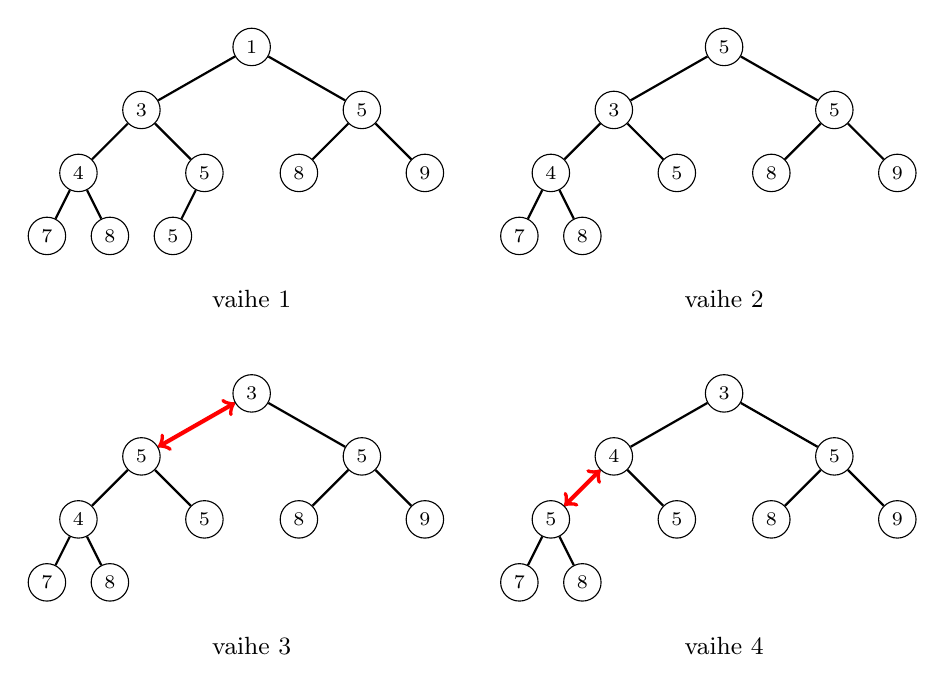
\begin{tikzpicture}[scale=0.4]
\scriptsize
\begin{scope}
\node[draw, circle] (1) at (0,0) {$1$};
\node[draw, circle] (2) at (-3.5,-2) {$3$};
\node[draw, circle] (3) at (3.5,-2) {$5$};
\node[draw, circle] (4) at (-5.5,-4) {$4$};
\node[draw, circle] (5) at (-1.5,-4) {$5$};
\node[draw, circle] (6) at (1.5,-4) {$8$};
\node[draw, circle] (7) at (5.5,-4) {$9$};
\node[draw, circle] (8) at (-6.5,-6) {$7$};
\node[draw, circle] (9) at (-4.5,-6) {$8$};
\node[draw, circle] (10) at (-2.5,-6) {$5$};
\path[draw,thick,-] (1) -- (2);
\path[draw,thick,-] (1) -- (3);
\path[draw,thick,-] (2) -- (4);
\path[draw,thick,-] (2) -- (5);
\path[draw,thick,-] (3) -- (6);
\path[draw,thick,-] (3) -- (7);
\path[draw,thick,-] (4) -- (8);
\path[draw,thick,-] (4) -- (9);
\path[draw,thick,-] (5) -- (10);
\node at (0,-8) {\small vaihe $1$};
\end{scope}
\begin{scope}[xshift=15cm]
\node[draw, circle] (1) at (0,0) {$5$};
\node[draw, circle] (2) at (-3.5,-2) {$3$};
\node[draw, circle] (3) at (3.5,-2) {$5$};
\node[draw, circle] (4) at (-5.5,-4) {$4$};
\node[draw, circle] (5) at (-1.5,-4) {$5$};
\node[draw, circle] (6) at (1.5,-4) {$8$};
\node[draw, circle] (7) at (5.5,-4) {$9$};
\node[draw, circle] (8) at (-6.5,-6) {$7$};
\node[draw, circle] (9) at (-4.5,-6) {$8$};
\path[draw,thick,-] (1) -- (2);
\path[draw,thick,-] (1) -- (3);
\path[draw,thick,-] (2) -- (4);
\path[draw,thick,-] (2) -- (5);
\path[draw,thick,-] (3) -- (6);
\path[draw,thick,-] (3) -- (7);
\path[draw,thick,-] (4) -- (8);
\path[draw,thick,-] (4) -- (9);
\node at (0,-8) {\small vaihe $2$};
\end{scope}
\begin{scope}[yshift=-11cm]
\node[draw, circle] (1) at (0,0) {$3$};
\node[draw, circle] (2) at (-3.5,-2) {$5$};
\node[draw, circle] (3) at (3.5,-2) {$5$};
\node[draw, circle] (4) at (-5.5,-4) {$4$};
\node[draw, circle] (5) at (-1.5,-4) {$5$};
\node[draw, circle] (6) at (1.5,-4) {$8$};
\node[draw, circle] (7) at (5.5,-4) {$9$};
\node[draw, circle] (8) at (-6.5,-6) {$7$};
\node[draw, circle] (9) at (-4.5,-6) {$8$};
\path[draw,thick,-] (1) -- (2);
\path[draw,thick,-] (1) -- (3);
\path[draw,thick,-] (2) -- (4);
\path[draw,thick,-] (2) -- (5);
\path[draw,thick,-] (3) -- (6);
\path[draw,thick,-] (3) -- (7);
\path[draw,thick,-] (4) -- (8);
\path[draw,thick,-] (4) -- (9);
\node at (0,-8) {\small vaihe $3$};
\path[draw,thick,<->,red,line width=1.5pt] (1) -- (2);
\end{scope}
\begin{scope}[yshift=-11cm,xshift=15cm]
\node[draw, circle] (1) at (0,0) {$3$};
\node[draw, circle] (2) at (-3.5,-2) {$4$};
\node[draw, circle] (3) at (3.5,-2) {$5$};
\node[draw, circle] (4) at (-5.5,-4) {$5$};
\node[draw, circle] (5) at (-1.5,-4) {$5$};
\node[draw, circle] (6) at (1.5,-4) {$8$};
\node[draw, circle] (7) at (5.5,-4) {$9$};
\node[draw, circle] (8) at (-6.5,-6) {$7$};
\node[draw, circle] (9) at (-4.5,-6) {$8$};
\path[draw,thick,-] (1) -- (2);
\path[draw,thick,-] (1) -- (3);
\path[draw,thick,-] (2) -- (4);
\path[draw,thick,-] (2) -- (5);
\path[draw,thick,-] (3) -- (6);
\path[draw,thick,-] (3) -- (7);
\path[draw,thick,-] (4) -- (8);
\path[draw,thick,-] (4) -- (9);
\node at (0,-8) {\small vaihe $4$};
\path[draw,thick,<->,red,line width=1.5pt] (2) -- (4);
\end{scope}
\end{tikzpicture}
\caption{Poistamme keon juuressa olevan alkion korvaamalla sen viimeisellä alkiolla
ja laskettamalla sitä alaspäin puussa.}
\label{fig:kekpoi}
\end{figure}

Kuva \ref{fig:kekpoi} näyttää, kuinka poistamme
esimerkkikeostamme pienimmän alkion eli juuressa
olevan alkion 1.
Aluksi korvaamme alkion 1
keon viimeisellä alkiolla 5 ja poistamme keosta
alkiolle 5 kuuluneen solmun.
Tämän jälkeen vaihdamme keskenään alkion 5
ja sen vasemman lapsen alkion 3,
ja sitten vielä alkion 5 ja sen vasemman lapsen alkion 4.
Tämän jälkeen kekoehto on voimassa ja olemme onnistuneet
poistamaan pienimmän alkion keosta.

Alkion poistaminen keosta vie aikaa $O(\log n)$,
koska keossa on $O(\log n)$ tasoa ja kuljemme polkua
alaspäin keon huipulta pohjaa kohden.

\section{Lisää keosta}

Koska keko on tallennettu taulukkona,
voimme tulkita minkä tahansa taulukon kekona,
kunhan vain kekoehto on voimassa taulukon kaikissa kohdissa.
Käymme seuraavaksi läpi menetelmän, jonka avulla voimme
\emph{muuttaa} taulukon keoksi $O(n)$-ajassa.
Tämän jälkeen tutustumme kekojärjestämiseen,
joka on $O(n \log n)$-aikainen järjestämisalgoritmi.

\subsection{Taulukosta keoksi}

Oletetaan, että meillä on $n$ alkiota sisältävä taulukko
ja haluamme muuttaa sen keoksi.
Suoraviivainen tapa on luoda tyhjä keko ja
lisätä jokainen taulukon alkio siihen erikseen $O(\log n)$-ajassa.
Tällä tavalla saamme rakennettua keon $O(n \log n)$-ajassa.
Osoittautuu kuitenkin, että pystymme myös muuttamaan taulukon
\emph{suoraan} keoksi tehokkaammin ajassa $O(n)$.

Ideana on järjestää alkuperäisen taulukon alkioita uudestaan niin,
että kekoehto tulee voimaan taulukon jokaiseen kohtaan --
jolloin taulukko on muuttunut keoksi.
Käymme läpi taulukon alkiot lopusta alkuun ja varmistamme
jokaisessa kohdassa, että kekoehto on voimassa kyseisestä
kohdasta alkavassa alipuussa.
Jos kekoehto ei ole voimassa, korjaamme sen laskettamalla
kyseisen kohdan alkiota alaspäin keossa.
Kun lopulta pääsemme taulukon alkuun, kekoehto on voimassa
koko taulukossa.

\begin{figure}
\center
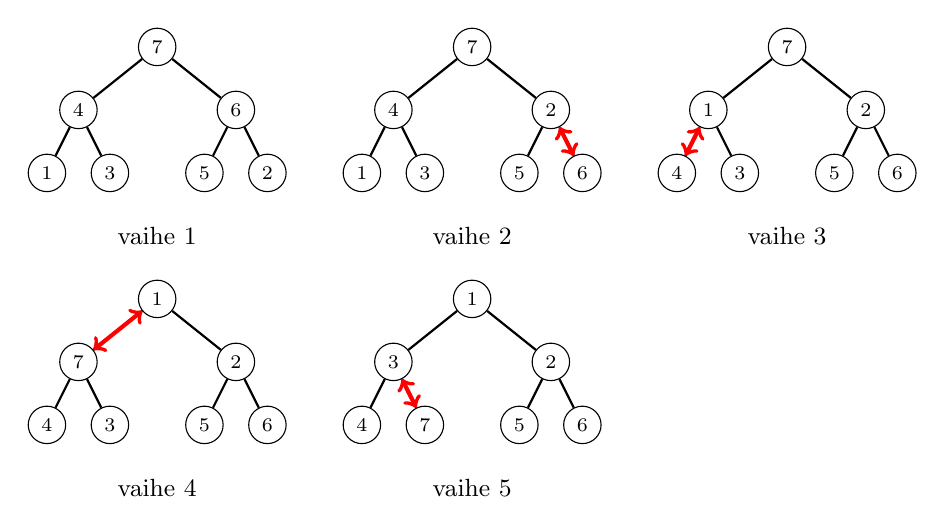
\begin{tikzpicture}[scale=0.4]
\scriptsize
\begin{scope}
\node[draw, circle] (1) at (0,0) {$7$};
\node[draw, circle] (2) at (-2.5,-2) {$4$};
\node[draw, circle] (3) at (2.5,-2) {$6$};
\node[draw, circle] (4) at (-3.5,-4) {$1$};
\node[draw, circle] (5) at (-1.5,-4) {$3$};
\node[draw, circle] (6) at (1.5,-4) {$5$};
\node[draw, circle] (7) at (3.5,-4) {$2$};
\path[draw,thick,-] (1) -- (2);
\path[draw,thick,-] (1) -- (3);
\path[draw,thick,-] (2) -- (4);
\path[draw,thick,-] (2) -- (5);
\path[draw,thick,-] (3) -- (6);
\path[draw,thick,-] (3) -- (7);
\node at (0,-6) {\small vaihe $1$};
\end{scope}
\begin{scope}[xshift=10cm]
\node[draw, circle] (1) at (0,0) {$7$};
\node[draw, circle] (2) at (-2.5,-2) {$4$};
\node[draw, circle] (3) at (2.5,-2) {$2$};
\node[draw, circle] (4) at (-3.5,-4) {$1$};
\node[draw, circle] (5) at (-1.5,-4) {$3$};
\node[draw, circle] (6) at (1.5,-4) {$5$};
\node[draw, circle] (7) at (3.5,-4) {$6$};
\path[draw,thick,-] (1) -- (2);
\path[draw,thick,-] (1) -- (3);
\path[draw,thick,-] (2) -- (4);
\path[draw,thick,-] (2) -- (5);
\path[draw,thick,-] (3) -- (6);
\path[draw,thick,-] (3) -- (7);
\node at (0,-6) {\small vaihe $2$};
\path[draw,thick,<->,red,line width=1.5pt] (3) -- (7);
\end{scope}
\begin{scope}[xshift=20cm]
\node[draw, circle] (1) at (0,0) {$7$};
\node[draw, circle] (2) at (-2.5,-2) {$1$};
\node[draw, circle] (3) at (2.5,-2) {$2$};
\node[draw, circle] (4) at (-3.5,-4) {$4$};
\node[draw, circle] (5) at (-1.5,-4) {$3$};
\node[draw, circle] (6) at (1.5,-4) {$5$};
\node[draw, circle] (7) at (3.5,-4) {$6$};
\path[draw,thick,-] (1) -- (2);
\path[draw,thick,-] (1) -- (3);
\path[draw,thick,-] (2) -- (4);
\path[draw,thick,-] (2) -- (5);
\path[draw,thick,-] (3) -- (6);
\path[draw,thick,-] (3) -- (7);
\node at (0,-6) {\small vaihe $3$};
\path[draw,thick,<->,red,line width=1.5pt] (2) -- (4);
\end{scope}
\begin{scope}[yshift=-8cm]
\node[draw, circle] (1) at (0,0) {$1$};
\node[draw, circle] (2) at (-2.5,-2) {$7$};
\node[draw, circle] (3) at (2.5,-2) {$2$};
\node[draw, circle] (4) at (-3.5,-4) {$4$};
\node[draw, circle] (5) at (-1.5,-4) {$3$};
\node[draw, circle] (6) at (1.5,-4) {$5$};
\node[draw, circle] (7) at (3.5,-4) {$6$};
\path[draw,thick,-] (1) -- (2);
\path[draw,thick,-] (1) -- (3);
\path[draw,thick,-] (2) -- (4);
\path[draw,thick,-] (2) -- (5);
\path[draw,thick,-] (3) -- (6);
\path[draw,thick,-] (3) -- (7);
\node at (0,-6) {\small vaihe $4$};
\path[draw,thick,<->,red,line width=1.5pt] (1) -- (2);
\end{scope}
\begin{scope}[yshift=-8cm,xshift=10cm]
\node[draw, circle] (1) at (0,0) {$1$};
\node[draw, circle] (2) at (-2.5,-2) {$3$};
\node[draw, circle] (3) at (2.5,-2) {$2$};
\node[draw, circle] (4) at (-3.5,-4) {$4$};
\node[draw, circle] (5) at (-1.5,-4) {$7$};
\node[draw, circle] (6) at (1.5,-4) {$5$};
\node[draw, circle] (7) at (3.5,-4) {$6$};
\path[draw,thick,-] (1) -- (2);
\path[draw,thick,-] (1) -- (3);
\path[draw,thick,-] (2) -- (4);
\path[draw,thick,-] (2) -- (5);
\path[draw,thick,-] (3) -- (6);
\path[draw,thick,-] (3) -- (7);
\node at (0,-6) {\small vaihe $5$};
\path[draw,thick,<->,red,line width=1.5pt] (2) -- (5);
\end{scope}
\end{tikzpicture}
\caption{Muutamme taulukon keoksi korjaamalla kekoehdon alipuissa.}
\label{fig:taukek}
\end{figure}

Kuva \ref{fig:taukek} näyttää esimerkin, jossa muutamme taulukon
$[7,4,6,1,3,5,2]$ minimikeoksi.
Kun tulkitsemme taulukon kekona, kekoehto on aluksi
rikki monessa taulukon kohdassa.
Ensin korjaamme kekoehdon tason 2 alipuissa vaihtamalla
keskenään alkiot 2 ja 6 ja sitten alkiot 1 ja 4.
Tämän jälkeen korjaamme kekoehdon tason 1 alipuussa
eli koko keossa laskettamalla alkion 7 keon huipulta pohjalle.
Nyt kekoehto on voimassa kaikkialla taulukossa,
joten olemme onnistuneet muuttamaan taulukon keoksi.

Miksi sitten tämä vie aikaa vain $O(n)$?
Oletetaan, että keossa on $h$ tasoa ja kaikki
tasot ovat täynnä solmuja, eli keossa on $n=2^h-1$ solmua.
Laskemme jokaiselle tasolle, montako alkiota laskeutuu
enintään jostakin tämän tason solmusta alaspäin.
Ensinnäkin tasolta 1 tasolle 2 laskeutuu enintään 1 alkio --
juuressa oleva alkio.
Vastaavasti
tasolta 2 tasolle 3 laskeutuu enintään $1+2$ alkiota
ja
tasolta 3 tasolle 4 laskeutuu enintään $1+2+4$ alkiota.
Yleisemmin tasolta $k$ tasolle $k+1$ laskeutuu
enintään $1+2+\dots+2^{k-1} = 2^k-1$ alkiota
Koska tasoja on $h$ ja alimmalta tasolta ei voi laskeutua alaspäin,
kokonaistyömäärä on enintään
\[(2^1-1)+(2^2-1)+\dots+(2^{h-1}-1)=2^h-h-1 \le n,\]
joten aikaa kuluu vain $O(n)$.

\subsection{Kekojärjestäminen}

\index{kekojärjestäminen}

\emph{Kekojärjestäminen} (\emph{heap sort}) on järjestämisalgoritmi,
jonka toiminta perustuu kekoon.
Ideana on muuttaa järjestettävä taulukko ensin keoksi
ja sen jälkeen poistaa alkiot keosta yksi kerrallaan
järjestyksessä.
Kekojärjestäminen vie aikaa $O(n \log n)$,
koska taulukon muuttaminen keoksi vie aikaa $O(n)$
ja $n$ alkion poistaminen keosta vie aikaa $O(n \log n)$.

\begin{figure}
\center
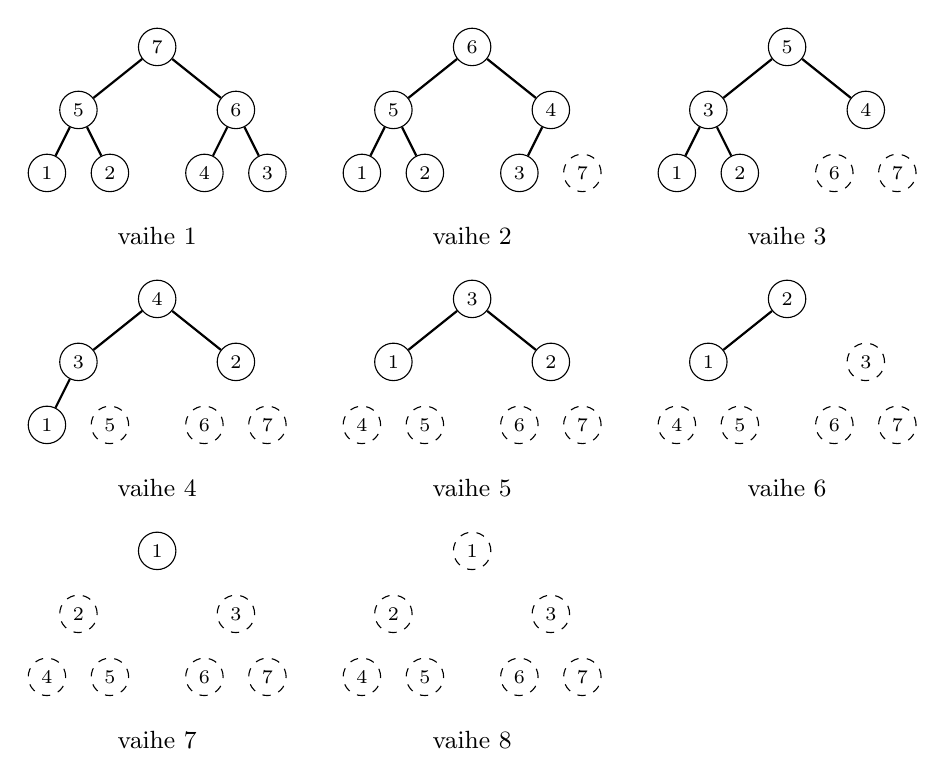
\begin{tikzpicture}[scale=0.4]
\scriptsize
\begin{scope}
\node[draw, circle] (1) at (0,0) {$7$};
\node[draw, circle] (2) at (-2.5,-2) {$5$};
\node[draw, circle] (3) at (2.5,-2) {$6$};
\node[draw, circle] (4) at (-3.5,-4) {$1$};
\node[draw, circle] (5) at (-1.5,-4) {$2$};
\node[draw, circle] (6) at (1.5,-4) {$4$};
\node[draw, circle] (7) at (3.5,-4) {$3$};
\path[draw,thick,-] (1) -- (2);
\path[draw,thick,-] (1) -- (3);
\path[draw,thick,-] (2) -- (4);
\path[draw,thick,-] (2) -- (5);
\path[draw,thick,-] (3) -- (6);
\path[draw,thick,-] (3) -- (7);
\node at (0,-6) {\small vaihe $1$};
\end{scope}
\begin{scope}[xshift=10cm]
\node[draw, circle] (1) at (0,0) {$6$};
\node[draw, circle] (2) at (-2.5,-2) {$5$};
\node[draw, circle] (3) at (2.5,-2) {$4$};
\node[draw, circle] (4) at (-3.5,-4) {$1$};
\node[draw, circle] (5) at (-1.5,-4) {$2$};
\node[draw, circle] (6) at (1.5,-4) {$3$};
\node[draw, circle, dashed] (7) at (3.5,-4) {$7$};
\path[draw,thick,-] (1) -- (2);
\path[draw,thick,-] (1) -- (3);
\path[draw,thick,-] (2) -- (4);
\path[draw,thick,-] (2) -- (5);
\path[draw,thick,-] (3) -- (6);
\node at (0,-6) {\small vaihe $2$};
\end{scope}
\begin{scope}[xshift=20cm]
\node[draw, circle] (1) at (0,0) {$5$};
\node[draw, circle] (2) at (-2.5,-2) {$3$};
\node[draw, circle] (3) at (2.5,-2) {$4$};
\node[draw, circle] (4) at (-3.5,-4) {$1$};
\node[draw, circle] (5) at (-1.5,-4) {$2$};
\node[draw, circle, dashed] (6) at (1.5,-4) {$6$};
\node[draw, circle, dashed] (7) at (3.5,-4) {$7$};
\path[draw,thick,-] (1) -- (2);
\path[draw,thick,-] (1) -- (3);
\path[draw,thick,-] (2) -- (4);
\path[draw,thick,-] (2) -- (5);
\node at (0,-6) {\small vaihe $3$};
\end{scope}
\begin{scope}[xshift=0cm,yshift=-8cm]
\node[draw, circle] (1) at (0,0) {$4$};
\node[draw, circle] (2) at (-2.5,-2) {$3$};
\node[draw, circle] (3) at (2.5,-2) {$2$};
\node[draw, circle] (4) at (-3.5,-4) {$1$};
\node[draw, circle, dashed] (5) at (-1.5,-4) {$5$};
\node[draw, circle, dashed] (6) at (1.5,-4) {$6$};
\node[draw, circle, dashed] (7) at (3.5,-4) {$7$};
\path[draw,thick,-] (1) -- (2);
\path[draw,thick,-] (1) -- (3);
\path[draw,thick,-] (2) -- (4);
\node at (0,-6) {\small vaihe $4$};
\end{scope}
\begin{scope}[xshift=10cm,yshift=-8cm]
\node[draw, circle] (1) at (0,0) {$3$};
\node[draw, circle] (2) at (-2.5,-2) {$1$};
\node[draw, circle] (3) at (2.5,-2) {$2$};
\node[draw, circle, dashed] (4) at (-3.5,-4) {$4$};
\node[draw, circle, dashed] (5) at (-1.5,-4) {$5$};
\node[draw, circle, dashed] (6) at (1.5,-4) {$6$};
\node[draw, circle, dashed] (7) at (3.5,-4) {$7$};
\path[draw,thick,-] (1) -- (2);
\path[draw,thick,-] (1) -- (3);
\node at (0,-6) {\small vaihe $5$};
\end{scope}
\begin{scope}[xshift=20cm,yshift=-8cm]
\node[draw, circle] (1) at (0,0) {$2$};
\node[draw, circle] (2) at (-2.5,-2) {$1$};
\node[draw, circle, dashed] (3) at (2.5,-2) {$3$};
\node[draw, circle, dashed] (4) at (-3.5,-4) {$4$};
\node[draw, circle, dashed] (5) at (-1.5,-4) {$5$};
\node[draw, circle, dashed] (6) at (1.5,-4) {$6$};
\node[draw, circle, dashed] (7) at (3.5,-4) {$7$};
\path[draw,thick,-] (1) -- (2);
\node at (0,-6) {\small vaihe $6$};
\end{scope}
\begin{scope}[xshift=0cm,yshift=-16cm]
\node[draw, circle] (1) at (0,0) {$1$};
\node[draw, circle, dashed] (2) at (-2.5,-2) {$2$};
\node[draw, circle, dashed] (3) at (2.5,-2) {$3$};
\node[draw, circle, dashed] (4) at (-3.5,-4) {$4$};
\node[draw, circle, dashed] (5) at (-1.5,-4) {$5$};
\node[draw, circle, dashed] (6) at (1.5,-4) {$6$};
\node[draw, circle, dashed] (7) at (3.5,-4) {$7$};
\node at (0,-6) {\small vaihe $7$};
\end{scope}
\begin{scope}[xshift=10cm,yshift=-16cm]
\node[draw, circle, dashed] (1) at (0,0) {$1$};
\node[draw, circle, dashed] (2) at (-2.5,-2) {$2$};
\node[draw, circle, dashed] (3) at (2.5,-2) {$3$};
\node[draw, circle, dashed] (4) at (-3.5,-4) {$4$};
\node[draw, circle, dashed] (5) at (-1.5,-4) {$5$};
\node[draw, circle, dashed] (6) at (1.5,-4) {$6$};
\node[draw, circle, dashed] (7) at (3.5,-4) {$7$};
\node at (0,-6) {\small vaihe $8$};
\end{scope}
\end{tikzpicture}
\caption{Esimerkki kekojärjestämisestä.}
\label{fig:kekjar}
\end{figure}

Kuva \ref{fig:kekjar} näyttää esimerkin kekojärjestämisestä,
kun järjestämme taulukon $[5,2,3,1,7,4,6]$
pienimmästä suurimpaan.
Muutamme ensin taulukon maksimikeoksi,
jolloin taulukosta tulee $[7,5,6,1,2,4,3]$.
Tämän jälkeen poistamme yksi kerrallaan
keon juuressa olevan alkion vaihtamalla sen
keon viimeisen alkion kanssa.
Tämän seurauksena keosta poistuneet alkiot
(merkitty katkoviivoilla) muodostavat lopulta järjestetyn taulukon.

Olemme siis saaneet aikaan kolmannen $O(n \log n)$-aikaisen
järjestämis\-algoritmin lomitusjärjestämisen ja pikajärjestämisen rinnalle.
Kekojärjestä\-misen etuna on, että sen tilavaativuus on vain $O(1)$,
koska keon operaatiot käyttävät vain yksittäisiä muuttujia.
Kekojärjestäminen ei ole kuitenkaan käytännössä yhtä tehokas algoritmi
kuin lomitusjärjestäminen tai pikajärjestäminen,
minkä vuoksi se ei ole saavuttanut samanlaista asemaa
järjestämisalgoritmien joukossa.
Siinä on kuitenkin yksi kiinnostava ominaisuus:
jos haluamme selvittää vain taulukon $k$ pienintä tai suurinta
alkiota, tämä onnistuu ajassa $O(n+k \log n)$,
koska meidän riittää poistaa keosta $k$ kertaa
pienin tai suurin alkio ajassa $O(\log n)$.

\section{Ohjelmointikielten toteutukset}

\subsection{Java}

\index{prioriteettijono}

Javassa kekorakenteesta käytetään nimeä \emph{prioriteettijono} (\emph{priority queue}).
Tietorakenne \texttt{PriorityQueue}
toteuttaa binäärikeon, joka on oletuksena minimikeko.
Metodi \texttt{peek} hakee pienimmän alkion, ja
metodi \texttt{poll} hakee ja poistaa pienimmän alkion.

\begin{code}
PriorityQueue<Integer> jono = new PriorityQueue<>();
jono.add(5);
jono.add(3);
jono.add(8);
jono.add(7);
System.out.println(jono.peek()); // 3
System.out.println(jono.poll()); // 3
System.out.println(jono.poll()); // 5
\end{code}

Jos haluamme luoda prioriteettijonon, joka onkin
maksimikeko, voimme tehdä tämän seuraavasti:

\begin{code}
PriorityQueue<Integer> jono =
    new PriorityQueue<>(Collections.reverseOrder());
\end{code}

\subsection{Python}

Pythonin standardikirjaston moduulissa \texttt{heapq} on funktioita,
joiden avulla listaa voi käsitellä binäärikekona.
Toteutuksessa keko on minimikeko ja tavallisesta käytännöstä
poiketen keon kohdat on 0-indeksoitu eli keon pienin alkio on aina
listan kohdassa 0.

Seuraava koodi näyttää, miten voimme käsitellä kekoa:

\begin{code}
from heapq import heappush, heappop

jono = []
heappush(jono,5)
heappush(jono,3)
heappush(jono,8)
heappush(jono,7)
print(jono[0]) # 3
heappop(jono)
print(jono[0]) # 5
\end{code}

Lisäksi saatavilla on funktio \texttt{heapify},
joka muuttaa olemassa olevan listan minimikeoksi
lineaarisessa ajassa:

\begin{code}
from heapq import heapify, heappop

jono = [5,3,8,7]
heapify(jono)
print(jono[0]) # 3
heappop(jono)
print(jono[0]) # 5
\end{code}

\section{Tehokkuusvertailu}

Mitä hyötyä keosta oikeastaan on?
Meillähän on olemassa jo binäärihakupuu,
jonka avulla voimme toteuttaa kaikki keon operaatiot
ja \emph{enemmänkin}.
Keossa voimme hakea ja poistaa vain pienimmän tai suurimman alkion,
mutta binäärihakupuussa voimme käsitellä myös muita alkioita.

Keon etuna on, että siinä on tehokkaan taulukkototeutuksen
ansiosta pienemmät \emph{vakiokertoimet} kuin binäärihakupuussa.
Jos meille riittää, että voimme hakea ja poistaa
vain pienimmän tai suurimman alkion, voi siis olla hyvä
ratkaisu käyttää kekoa binäärihakupuun sijasta.
Mutta kuinka suuria erot ovat käytännössä?

Tästä antaa kuvaa seuraava testi,
jossa vertailemme keskenään Javan tietorakenteita
\texttt{PriorityQueue} ja \texttt{TreeSet}.
Testissä meillä on taulukko,
jossa on satunnaisessa järjestyksessä luvut $1,2,\dots,n$.
Lisäämme ensin taulukon $n/2$ ensimmäistä lukua joukkoon.
Tämän jälkeen käymme läpi loput $n/2$ lukua,
ja jokaisen luvun kohdalla lisäämme sen joukkoon ja
poistamme joukon pienimmän luvun.

Taulukko \ref{tab:kekver} näyttää testin tulokset.
Tämän testin perusteella näyttää siltä,
että keon käyttämisestä on todellista hyötyä,
koska \texttt{PriorityQueue} toimii 2–3
kertaa nopeammin kuin \texttt{TreeSet}.

\begin{table}
\center
\begin{tabular}{rrrr}
taulukon koko $n$ & \texttt{PriorityQueue} & \texttt{TreeSet} \\
\hline
$10^6$ & 0.29 s & 0.78 s \\
$2 \cdot 10^6$ & 0.71 s & 1.50 s \\
$4 \cdot 10^6$ & 1.56 s & 3.72 s \\
$8 \cdot 10^6$ & 3.68 s & 9.43 s \\
\end{tabular}
\caption{Algoritmien suoritusaikojen vertailu.}
\label{tab:kekver}
\end{table}

\chapter{Peruuttava haku}

\index{backtracking}
\emph{Peruuttava haku} (\emph{backtracking}) on menetelmä,
jonka avulla voimme käydä järjestelmällisesti kaikki yhdistelmät,
jotka voidaan muodostaa annetuista aineksista.
Peruuttava haku on raa'an voiman algoritmi,
jonka toteutus on yleensä suoraviivainen,
ja menetelmä on käyttökelpoinen silloin,
kun yhdistelmien määrä on niin pieni, että ehdimme käydä kaikki läpi.

Tässä luvussa tutustumme ensin peruuttavan haun algoritmeihin,
jotka käyvät läpi lukujen yhdistelmiä.
Tämän jälkeen näemme, miten peruuttavaa hakua voi käyttää
kahdessa vaikeammassa ongelmassa ja miten hakua voi tehostaa.
Lopuksi toteutamme pelin tekoälyn minimax-algoritmilla,
joka perustuu peruuttavaan hakuun.

\section{Silmukoista rekursioon}

Oletetaan, että haluamme käydä läpi kaikki $n$ luvun yhdistelmät,
joissa jokainen luku on kokonaisluku väliltä $1 \dots m$.
Tällaisia yhdistelmiä on yhteensä $m^n$,
koska kohtia on $n$ ja joka kohdassa luvun voi valita $m$ tavalla.
Esimerkiksi jos $n=3$ ja $m=4$, yhdistelmät ovat
$[1,1,1]$, $[1,1,2]$, $[1,1,3]$, $[1,1,4]$, $[1,2,1]$,
$[1,2,2]$, $[1,2,3]$, $[1,2,4]$, jne.

Jos lukujen määrä $n$ on etukäteen tiedossa, voimme
luoda $n$ sisäkkäistä silmukkaa, joista jokainen käy $m$ lukua läpi.
Esimerkiksi seuraava koodi käy läpi kaikki yhdistelmät
tapauksessa $n=3$:

\begin{code}
for a = 1 to m
    for b = 1 to m
        for c = 1 to m
            print(a,b,c)
\end{code}

Tämä on sinänsä mainio ratkaisu, mutta siinä on yksi ongelma:
lukujen määrä $n$ vaikuttaa silmukoiden määrään.
Jos haluaisimme muuttaa $n$:n arvoa, meidän täytyisi muuttaa
koodin silmukoiden määrää, mikä ei ole hyvä asia.
Peruuttavan haun avulla voimme kuitenkin toteuttaa ratkaisun
rekursiivisesti niin, että sama koodi toimii kaikille $n$:n arvoille.

\subsection{Haun toteuttaminen}

Seuraava rekursiivinen proseduuri \texttt{haku} muodostaa
yhdistelmiä peruuttavan haun avulla.
Parametri $k$ tarkoittaa kohtaa, johon seuraava luku asetetaan.
Jos $k=n$, jokin yhdistelmä on valmistunut, jolloin se tulostetaan.
Muuten haku käy läpi kaikki tavat sijoittaa kohtaan $k$ luku $1 \dots m$
ja jatkaa rekursiivisesti kohtaan $k+1$.
Haku lähtee käyntiin kutsulla \texttt{haku}(0),
ja \texttt{luvut} on $n$-kokoinen taulukko, johon yhdistelmä muodostetaan.

\begin{code}
procedure haku(k)
    if k == n
        print(luvut)
    else
        for i = 1 to m
            luvut[k] = i
            haku(k+1)
\end{code}

Kuva \ref{fig:perhak} näyttää, miten haku lähtee liikkeelle
tapauksessa $n=3$ ja $m=4$.
Merkki "$-$" tarkoittaa lukua, jota ei ole vielä valittu.
Haun ensimmäinen taso valitsee yhdistelmän
ensimmäisen luvun kohtaan $0$.
Tämän valintaan on neljä vaihtoehtoa,
koska mahdolliset luvut ovat $1 \dots 4$,
joten haku haarautuu neljään osaan.
Tämän jälkeen haku jatkaa rekursiivisesti eteenpäin
ja valitsee muihin kohtiin tulevat luvut.

\begin{figure}
\center
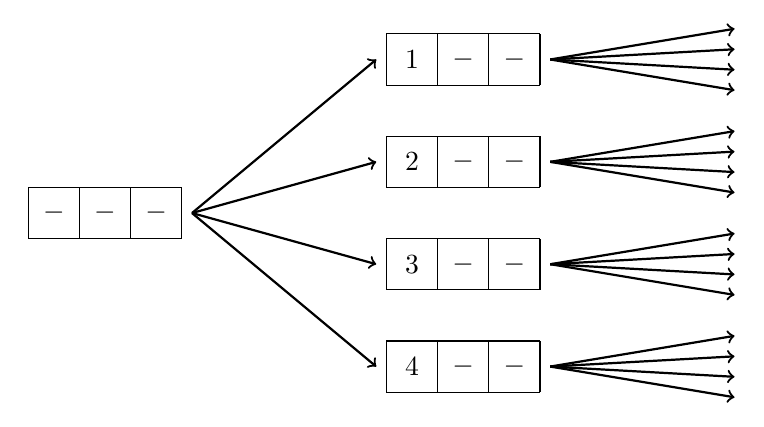
\begin{tikzpicture}[scale=.65]
    \draw (0,0) grid (3,1);
    \foreach \x/\v in {0/-,1/-,2/-} \node at (\x+0.5,0.5) {$\v$};

    \draw (7,-3) grid (10,-2);
    \foreach \x/\v in {0/1,1/-,2/-} \node at (\x+7.5,3.5) {$\v$};
    \draw (7,-1) grid (10,0);
    \foreach \x/\v in {0/2,1/-,2/-} \node at (\x+7.5,1.5) {$\v$};
    \draw (7,1) grid (10,2);
    \foreach \x/\v in {0/3,1/-,2/-} \node at (\x+7.5,-0.5) {$\v$};
    \draw (7,3) grid (10,4);
    \foreach \x/\v in {0/4,1/-,2/-} \node at (\x+7.5,-2.5) {$\v$};

    \draw[->,thick] (3.2,0.5) -- (6.8,3.5);
    \draw[->,thick] (3.2,0.5) -- (6.8,1.5);
    \draw[->,thick] (3.2,0.5) -- (6.8,-0.5);
    \draw[->,thick] (3.2,0.5) -- (6.8,-2.5);
    
    \foreach \y in {3.5,1.5,-0.5,-2.5} \foreach \z in {0.6,0.2,-0.2,-0.6}
        \draw[->,thick] (10.2,\y) -- (13.8,\y+\z);
\end{tikzpicture}
\caption{Yhdistelmien muodostaminen alkaa ($n=3$ ja $m=4$).}
\label{fig:perhak}
\end{figure}

Voimme arvioida algoritmin tehokkuutta laskemalla,
montako kertaa proseduuria \texttt{haku} kutsutaan yhteensä haun aikana.
Proseduuria kutsutaan kerran parametrilla $0$,
$m$ kertaa parametrilla $1$, $m^2$ kertaa parametrilla $2$, jne.,
joten kutsujen määrä on yhteensä
\[
1+m+m^2+\dots+m^n = \frac{m^{n+1}-1}{m-1} = O(m^n).
\]
Tästä näkee, että kutsujen yhteismäärä on samaa luokkaa kuin
viimeisen tason kutsujen määrä.
Viimeisellä tasolla tehdäänkin enemmän kutsuja kuin
kaikilla muilla tasoilla yhteensä.

\subsection{Osajoukkojen läpikäynti}

Tarkastellaan sitten tilannetta,
jossa haluamme käydä läpi kaikki $n$ alkion
joukon \emph{osajoukot}.
Osajoukkoja on yhteensä $2^n$,
koska jokainen alkio joko kuuluu tai ei kuulu osajoukkoon.
Esimerkiksi joukon $\{2,3,5,9\}$ osajoukkoja ovat
$\{2,5\}$ ja $\{3,5,9\}$.

Osoittautuu, että voimme muodostaa osajoukot
käymällä läpi kaikki $n$ luvun yhdistelmät,
joissa jokainen luku on 0 tai 1.
Ideana on, että jokainen yhdistelmän luku kertoo,
kuuluuko tietty alkio osajoukkoon,
Alkio kuuluu osajoukkoon tarkalleen silloin,
kun sen kohdalla on luku 1.
Esimerkiksi kun joukkona on $\{2,3,5,9\}$,
yhdistelmä $[1,0,1,0]$ vastaa
osajoukkoa $\{2,5\}$ ja
yhdistelmä $[0,1,1,1]$ vastaa osajoukkoa $\{3,5,9\}$.

Seuraava koodi näyttää, miten voimme käydä osajoukot
läpi peruuttavan haun avulla.
Proseduuri \texttt{haku} valitsee,
otetaanko kohdassa $k$ oleva alkio mukaan osajoukkoon vai ei,
ja merkitsee tämän tiedon taulukkoon \texttt{valinta}.
Kuten ennenkin, haku lähtee käyntiin kutsulla \texttt{haku}$(0)$.

\begin{code}
procedure haku(k)
    if k == n
        // käsittele osajoukko
    else
        for i = 0 to 1
            valinta[k] = i
            haku(k+1)
\end{code}

\subsection{Permutaatioiden läpikäynti}

Peruuttavan haun avulla voimme myös käydä läpi joukon
\emph{permutaatiot} eli erilaiset järjestykset.
Kun joukossa on $n$ alkiota, siitä voidaan muodostaa
kaikkiaan $n!$ permutaatiota.
Esimerkiksi joukon $\{1,2,3,4\}$ permutaatioita ovat
$\{2,4,1,3\}$ ja $\{4,3,1,2\}$.

Tässä tilanteessa haluamme käydä läpi $n$ luvun yhdistelmiä,
joissa jokainen luku on väliltä $1 \dots n$
ja lisäksi mikään luku ei toistu.
Saamme tämän aikaan lisäämällä hakuun uuden taulukon
\texttt{mukana}, joka kertoo, onko tietty luku jo mukana.
Joka vaiheessa haku valitsee yhdistelmään vain sellaisia lukuja,
joita ei ole valittu siihen aiemmin.

\begin{code}
procedure haku(k)
    if k == n
        print(luvut)
    else
        for i = 1 to n
            if not mukana[i]
                mukana[i] = true
                luvut[k] = i
                haku(k+1)
                mukana[i] = false
\end{code}

\section{Esimerkkejä}

Käymme seuraavaksi läpi kaksi vaativampaa esimerkkiä
peruuttavan haun soveltamisesta.
Ratkaisemme ensin shakkiin liittyvän ongelman,
ja tämän jälkeen etsimme parhaan tavan
työtehtävien jakamiseen.
Molemmissa sovelluksissa näemme myös,
miten peruuttavaa hakua voi tehostaa.

\subsection{Kuningatarongelma}

Tehtävämme on laskea, monellako tavalla
$n \times n$ -shakkilaudalle voidaan asettaa $n$ kuningatarta
niin, etteivät mitkään kaksi kuningatarta uhkaa toisiaan.
Shakissa kuningattaret voivat uhata toisiaan
vaaka-, pysty- tai vinosuuntaisesti.
Esimerkiksi tapauksessa $n=4$ mahdollisia sijoitustapoja on kaksi,
jotka on esitetty kuvassa \ref{fig:kuning}.

\begin{figure}[h]
\center
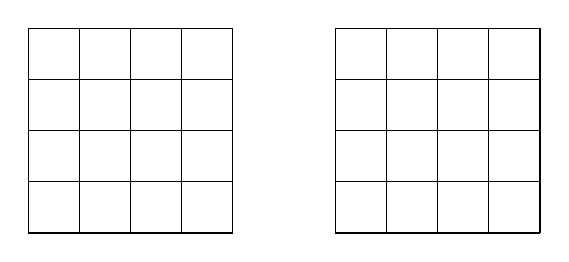
\begin{tikzpicture}[scale=.65]
  \begin{scope}
    \draw (0, 0) grid (4, 4);
    \node at (1.5,3.5) {$\symqueen$};
    \node at (3.5,2.5) {$\symqueen$};
    \node at (0.5,1.5) {$\symqueen$};
    \node at (2.5,0.5) {$\symqueen$};

    \draw (6, 0) grid (10, 4);
    \node at (6+2.5,3.5) {$\symqueen$};
    \node at (6+0.5,2.5) {$\symqueen$};
    \node at (6+3.5,1.5) {$\symqueen$};
    \node at (6+1.5,0.5) {$\symqueen$};
  \end{scope}
\end{tikzpicture}
\caption{Kuningatarongelman ratkaisut tapauksessa $n=4$.}
\label{fig:kuning}
\end{figure}

Voimme ratkaista tehtävän toteuttamalla algoritmin,
joka käy laudan läpi ylhäältä alaspäin ja asettaa yhden kuningattaren
jokaiselle riville.
Kuva \ref{fig:hakupuu} esittää haun toimintaa tapauksessa $n=4$.
Ensimmäisen rivin kuningatar voidaan asettaa mihin tahansa sarakkeeseen,
mutta seuraavilla riveillä aiemmat valinnat rajoittavat hakua.
Kuvassa näkyy toisen kuningattaren sijoittaminen,
kun ensimmäinen kuningatar on toisessa sarakkeessa.
Tällöin ainoa vaihtoehto on, että toinen kuningatar on viimeisessä sarakkeessa,
koska kaikissa muissa tapauksissa kuningattaret uhkaisivat toisiaan.


\begin{figure}
\center
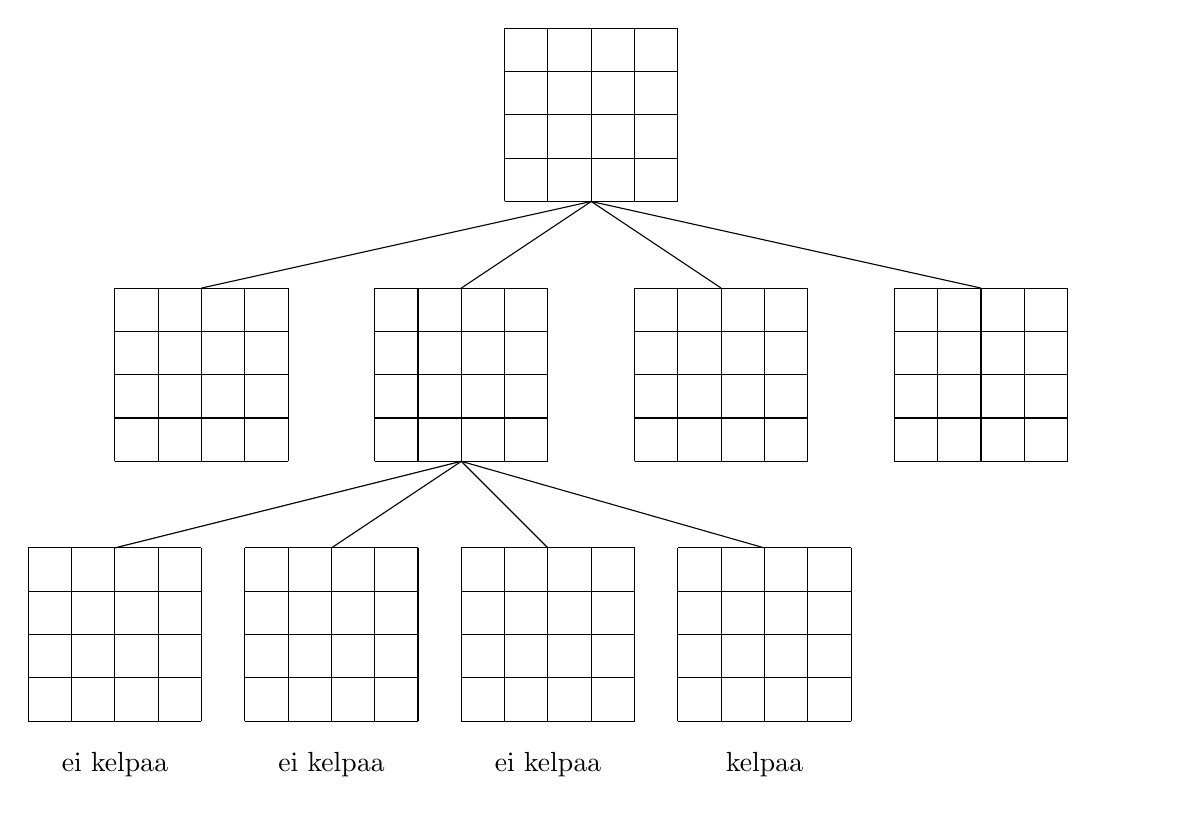
\begin{tikzpicture}[scale=.55]
  \begin{scope}
    \draw (0, 0) grid (4, 4);

    \draw (-9, -6) grid (-5, -2);
    \draw (-3, -6) grid (1, -2);
    \draw (3, -6) grid (7, -2);
    \draw (9, -6) grid (13, -2);

    \node at (-9+0.5,-3+0.5) {$\symqueen$};
    \node at (-3+1+0.5,-3+0.5) {$\symqueen$};
    \node at (3+2+0.5,-3+0.5) {$\symqueen$};
    \node at (9+3+0.5,-3+0.5) {$\symqueen$};

    \draw (2,0) -- (-7,-2);
    \draw (2,0) -- (-1,-2);
    \draw (2,0) -- (5,-2);
    \draw (2,0) -- (11,-2);

    \draw (-11, -12) grid (-7, -8);
    \draw (-6, -12) grid (-2, -8);
    \draw (-1, -12) grid (3, -8);
    \draw (4, -12) grid (8, -8);
    \draw[white] (11, -12) grid (15, -8);
    \node at (-11+1+0.5,-9+0.5) {$\symqueen$};
    \node at (-6+1+0.5,-9+0.5) {$\symqueen$};
    \node at (-1+1+0.5,-9+0.5) {$\symqueen$};
    \node at (4+1+0.5,-9+0.5) {$\symqueen$};
    \node at (-11+0+0.5,-10+0.5) {$\symqueen$};
    \node at (-6+1+0.5,-10+0.5) {$\symqueen$};
    \node at (-1+2+0.5,-10+0.5) {$\symqueen$};
    \node at (4+3+0.5,-10+0.5) {$\symqueen$};

    \draw (-1,-6) -- (-9,-8);
    \draw (-1,-6) -- (-4,-8);
    \draw (-1,-6) -- (1,-8);
    \draw (-1,-6) -- (6,-8);
    
    \node at (-9,-13) {ei kelpaa};
    \node at (-4,-13) {ei kelpaa};
    \node at (1,-13) {ei kelpaa};
    \node at (6,-13) {kelpaa};    
  \end{scope}
\end{tikzpicture}
\caption{Peruuttavan haun toiminta kuningatarongelmassa.}
\label{fig:hakupuu}
\end{figure}


Seuraava proseduuri \texttt{haku} esittää peruuttavan haun algoritmin,
joka laskee kuningatarongelman ratkaisut:

\begin{code}
procedure haku(y)
    if y == n
        laskuri += 1
    else
        for x = 0 to n-1
            if voi_sijoittaa(y,x)
                kohta[y] = x
                haku(y+1)
\end{code}

Oletamme, että laudan rivit ja sarakkeet on numeroitu $0 \dots n-1$.
Parametri $y$ kertoo, mille riville seuraava kuningatar tulee sijoittaa,
ja haku lähtee käyntiin kutsulla \texttt{haku}$(0)$.
Jos rivinä on $n$, kaikki kuningattaret on jo sijoitettu,
joten yksi ratkaisu on löytynyt.
Muuten suoritetaan silmukka, joka käy läpi mahdolliset sarakkeet
muuttujan $x$ avulla.
Jos kuningatar voidaan sijoittaa sarakkeeseen $x$
eli se ei uhkaa mitään aiemmin sijoitettua kuningatarta,
merkitään taulukkoon \texttt{kohta},
että kuningatar $y$ on sarakkeessa $x$,
ja haku jatkuu eteenpäin rekursiivisesti.

Lisäksi täytyy toteuttaa funktio \texttt{voi\_sijoittaa},
joka tutkii, voidaanko uusi kuningatar sijoittaa
rivin $y$ sarakkeeseen $x$.
Tämä voidaan selvittää taulukon \texttt{kohta} avulla näin:

\begin{code}
function voi_sijoittaa(y,x)
    for i = 0 to y-1
        if kohta[i] == x
            return false
        if abs(i-y) == abs(kohta[i]-x)
            return false
    return true
\end{code}

Funktio käy läpi kaikki aiemmin sijoitetut kuningattaret.
Jos aiemmin sijoitettu kuningatar olisi samassa sarakkeessa
(ensimmäinen ehto) tai samalla vinorivillä (toinen ehto)
kuin uusi kuningatar, tällaista sijoitusta ei voida tehdä
ja funktio palauttaa \texttt{false}.
Jos taas mikään aiempi kuningatar ei uhkaa uutta kuningatarta,
funktio palauttaa \texttt{true}.
Huomaa jälkimmäisessä ehdossa kätevä tapa tarkastaa
itseisarvon (funktio \texttt{abs}) avulla,
ovatko kuningattaret samalla vinorivillä.
Kuningattaret ovat samalla vinorivillä tarkalleen silloin,
kun niiden vaaka- ja pystysuuntaiset erot ovat samat.

\begin{table}
\center
\begin{tabular}{rr}
laudan koko $n$ & ratkaisujen määrä \\
\hline
1 & 1 \\
2 & 0 \\
3 & 0 \\
4 & 2 \\
5 & 10 \\
6 & 4 \\
7 & 40 \\
8 & 92 \\
9 & 352 \\
10 & 724 \\
\end{tabular}
\caption{Kuningatarongelman ratkaisujen määriä.}
\label{tab:kuning}
\end{table}

Nyt meillä on valmis algoritmi, jonka avulla voimme
käydä läpi kuningatarongelman ratkaisuja.
Taulukko \ref{tab:kuning} näyttää ratkaisujen määrät
tapauksissa $n=1 \dots 10$.
Algoritmi selvittää nämä tapaukset salamannopeasti,
mutta suuremmilla $n$:n arvoilla algoritmi alkaa viedä paljon aikaa.
Syynä tähän on, että kuningatarten sijoitustapojen
määrä kasvaa \emph{eksponentiaalisesti}
eli räjähdysmäisen nopeasti.
Esimerkiksi tapauksessa $n=20$ erilaisia ratkaisuja on jo yli 39 miljardia.

\index{symmetria}
Voimme kuitenkin koettaa nopeuttaa algoritmia parantamalla
sen toteutusta.
Yksi helppo tehostus on hyödyntää \emph{symmetriaa}.
Jokaista kuningatar\-ongelman ratkaisua vastaa toinen ratkaisu,
joka saadaan peilaamalla ratkaisu vaakasuuntaisesti.
Esimerkiksi kuvassa \ref{fig:kuning} ratkaisut voidaan muuttaa
toisikseen peilaamalla.
Tämän havainnon ansiosta voimme puolittaa algoritmin suoritusajan
lisäämällä vaatimuksen, että ensimmäinen kuningatar asetetaan
laudan vasempaan puoliskoon, ja kertomalla lopuksi vastauksen kahdella.
Jos laudan koko on pariton, täytyy vielä käsitellä erikseen tapaus,
jossa ensimmäinen kuningatar sijoitetaan keskisarakkeeseen.

Toinen mahdollinen tehostus olisi toteuttaa funktio
\texttt{voi\_sijoittaa} paremmin.
Tällä hetkellä se käy läpi kaikki aiemmin sijoitetut kuningattaret
ja vie aikaa $O(n)$, mutta funktio on mahdollista toteuttaa myös
ajassa $O(1)$ ottamalla käyttöön uusia aputaulukoita, joissa on tietoa,
mitkä sarakkeet ja vinorivit ovat uhattuina.
Tämä tehostus on kuitenkin vaikeampi toteuttaa kuin symmetristen ratkaisujen karsinta.

Kuningatarongelma on kuitenkin pohjimmiltaan vaikea ongelma,
eikä sen ratkaisuun tunneta mitään oleellisesti raakaa voimaa
parempaa tapaa.
Tällä hetkellä suurin tapaus, jonka ratkaisu tunnetaan, on $n=27$.
Tämän tapauksen käsittely vei aikaa noin vuoden laskentaklusterilla,
jossa oli suuri määrä rinnakkain laskevia
suorittimia\footnote{27-Queens Puzzle: Massively Parellel Enumeration and Solution Counting.
\url{https://github.com/preusser/q27}}.

\subsection{Työtehtävien jakaminen}

Tarkastellaan tilannetta, jossa on $n$ työtehtävää ja $n$ työntekijää.
Tehtävät tulee jakaa työntekijöille niin,
että jokainen työntekijä suorittaa tarkalleen yhden työtehtävän.
Jokaisesta työtehtävästä tiedetään,
paljonko sen suorittaminen maksaa kullakin työntekijällä,
ja tavoitteena on etsiä ratkaisu, jossa kokonaishinta on pienin mahdollinen.

\begin{figure}
\center
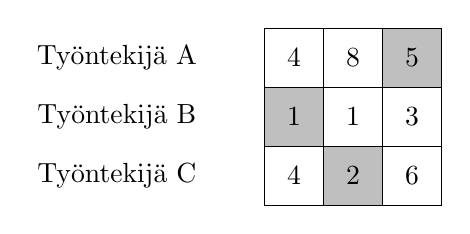
\begin{tikzpicture}[scale=0.75]
\fill[color=lightgray] (0,1) rectangle (1,2);
\fill[color=lightgray] (1,0) rectangle (2,1);
\fill[color=lightgray] (2,2) rectangle (3,3);
\draw (0,0) grid (3,3);
\node at (0.5,0.5) {$4$};
\node at (1.5,0.5) {$2$};
\node at (2.5,0.5) {$6$};
\node at (0.5,1.5) {$1$};
\node at (1.5,1.5) {$1$};
\node at (2.5,1.5) {$3$};
\node at (0.5,2.5) {$4$};
\node at (1.5,2.5) {$8$};
\node at (2.5,2.5) {$5$};
\node at (-2.5,2.5) {Työntekijä A};
\node at (-2.5,1.5) {Työntekijä B};
\node at (-2.5,0.5) {Työntekijä C};
\end{tikzpicture}
\caption{Optimaalinen tapa jakaa työtehtävät.}
\label{fig:tyoteh}
\end{figure}

Kuvassa \ref{fig:tyoteh} on esimerkki tilanteesta, jossa $n=3$.
Tässä optimaalinen tapa jakaa työtehtävät on,
että B suorittaa ensimmäisen työtehtävän,
C suorittaa toisen työtehtävän ja
A suorittaa kolmannen työtehtävän.
Tämän ratkaisun kustannus on $1+2+5=8$.

Oletamme, että työtehtävät ja työntekijät on numeroitu
$0 \dots n-1$ ja voimme lukea taulukosta \texttt{hinta}$[a][b]$,
paljonko työtehtävän $a$ suorittaminen maksaa
työntekijällä $b$.
Toteutamme peruuttavan haun algoritmin,
joka käy läpi työtehtävät järjestyksessä
ja valitsee jokaiselle työntekijän.

Seuraava proseduuri \texttt{haku} saa kaksi parametria:
$k$ on seuraavaksi käsitel\-tävä työtehtävä ja
$h$ on tähän mennessä muodostunut hinta.
Haku lähtee käyntiin kutsulla \texttt{haku}$(0,0)$.
Taulukko \texttt{mukana} pitää kirjaa,
mitkä työntekijät on jo valittu,
ja muuttujassa $p$ on yhteishinta
parhaassa tähän mennessä löytyneessä ratkaisussa.
Ennen hakua muuttujan $p$ arvona on $\infty$,
koska mi\-tään ratkaisua ei ole vielä olemassa.

\begin{code}
procedure haku(k,h)
    if k == n
        p = min(p,h)
    else
        for i = 0 to n-1
            if not mukana[i]
                mukana[i] = true
                haku(k+1,h+hinta[k][i])
                mukana[i] = false
\end{code}

Tämä on toimiva peruuttavan haun algoritmi,
ja haun päätteeksi muuttujassa $p$ on
parhaan ratkaisun yhteishinta.
Algoritmi on kuitenkin hidas, koska se käy aina läpi
kaikki $n!$ mahdollista ratkaisua.
Koska haluamme vain löytää parhaan ratkaisun emmekä
käydä läpi kaikkia ratkaisuja,
pystymme tehostamaan algoritmia lisäämään siihen ehdon,
joka lopettaa ratkaisun muodostamisen,
jos siitä ei voi tulla aiempaa parempi.

\index{branch and bound}
Testaamme seuraavaksi algoritmia tapauksella, jossa $n=20$ ja jokainen
taulukossa \texttt{hinta} oleva arvo on satunnainen
kokonaisluku välillä $1 \dots 100$.
Tässä tapauksessa edellä kuvattu algoritmi kävisi läpi 
\[20! = 2432902008176640000
\]
eri ratkaisua, mikä veisi aikaa \emph{satoja vuosia}.
Jotta voimme ratkaista tapauksen,
meidän täytyy parantaa algoritmia niin,
että se ei käy läpi kaikkia ratkaisuja
mutta löytää kuitenkin parhaan ratkaisun.
Tässä avuksi tulee tekniikka, josta käytetään usein nimeä
\emph{branch and bound}.
Siinä ideana on tehostaa peruuttavaa hakua
vähentämällä tutkittavien ratkaisujen määrää
sopivien ylä- ja alarajojen avulla.

Keskeinen havainto on, että voimme rajoittaa hakua muuttujan
$p$ avulla. Tässä muuttujassa on joka hetkellä
tähän mennessä parhaan löydetyn ratkaisun yhteishinta,
joten tämä on \emph{yläraja} sille, kuinka suuri parhaan ratkaisun
yhteishinta voi olla.
Toisaalta muuttujassa $h$ on muodosteilla olevan ratkaisun
hinta tässä vaiheessa, joka on \emph{alaraja} yhteishinnalle.
Jos $h \ge p$, muodosteilla olevasta ratkaisusta ei
voi tulla aiempaa parempaa. Voimmekin lisätä algoritmin alkuun
seuraavan tarkastuksen:

\begin{code}
procedure haku(k,h)
    if h >= p
        return
    ...
\end{code}

Tämän ansiosta ratkaisun muodostaminen päättyy heti,
jos sen hinta on yhtä suuri tai suurempi kuin parhaan
tiedossa olevan ratkaisun hinta.
Tämän tehostuksen avulla saamme ratkaistua
muodostamamme tapauksen testikoneella 152 sekunnissa.
Tämä on hieno saavutus, koska alkuperäinen algoritmi
ei kyennyt ratkaisemaan tapausta lainkaan.

Voimme kuitenkin tehostaa algoritmia vielä lisää
laskemalla tarkemman arvion alarajalle.
Muodosteilla olevan ratkaisun hinta on varmasti ainakin $h$,
mutta voimme lisäksi arvioida, paljonko myöhemmin valittavat
työntekijät lisäävät kustannusta:

\begin{code}
procedure haku(k,h)
    if h+arvio(k) >= p
        return
    ...
\end{code}

Tässä funktion \texttt{arvio} tulee antaa jokin arvio,
paljonko ainakin maksaa suorittaa jäljellä olevat työtehtävät $k \dots n-1$.
Yksi kätevä tapa saada arvio on käydä läpi jäljellä olevat
työtehtävät ja valita jokaisen tekijäksi \emph{halvin} työntekijä välittämättä
siitä, onko kyseinen työntekijä mahdollisesti valittu aiemmin.
Tämä antaa alarajan sille, paljonko kustannuksia on ainakin vielä tiedossa.
Tämän tehostuksen jälkeen tapauksen $n=20$ käsittely vie
testikoneella vain 7 sekuntia.
Paremman alarajan ansiosta saimme siis algoritmin
vielä noin 20 kertaa nopeammaksi verrattuna edelliseen versioon.

\section{Pelin tekoäly}

Peruuttavan haun avulla voi myös toteuttaa tekoälyn kahden pelaajan peliin,
kuten ristinollaan tai shakkiin.
Tällaisen tekoälyn täytyy pystyä päättämään,
miten toimia annetussa pelin tilanteessa.
Ideana on luoda haku, joka käy läpi
järjestelmällisesti mahdollisia siirtoja,
joita pelaajat voivat tehdä.

\subsection{Minimax-algoritmi}

\index{minimax-algoritmi}
\emph{Minimax-algoritmi} on peruuttavaan hakuun perustuva algoritmi,
joka valitsee tekoälyn siirron pelissä.
Se käy läpi pelinkulkuja tiettyyn syvyyteen asti,
arvioi pelitilanteet ja valitsee siirron,
joka takaa mahdollisimman hyvältä vaikuttavan tuloksen.
Algoritmin nimi tulee siitä, että se vuorotellen
\emph{minimoi} ja \emph{maksimoi} tulosta puun kerroksissa.

\begin{figure}
\center
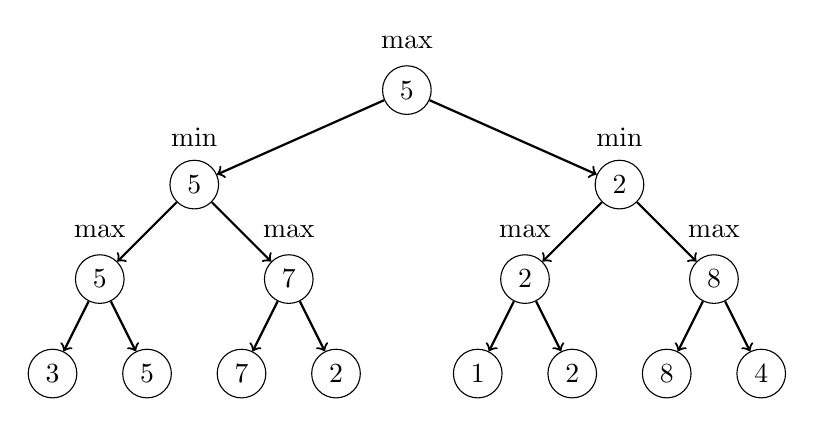
\begin{tikzpicture}[scale=0.6]
\node[draw, circle] (1) at (0,0) {$5$};
\node[draw, circle] (2) at (-4.5,-2) {$5$};
\node[draw, circle] (3) at (4.5,-2) {$2$};
\node[draw, circle] (4) at (-6.5,-4) {$5$};
\node[draw, circle] (5) at (-2.5,-4) {$7$};
\node[draw, circle] (6) at (2.5,-4) {$2$};
\node[draw, circle] (7) at (6.5,-4) {$8$};
\node[draw, circle] (8) at (-7.5,-6) {$3$};
\node[draw, circle] (9) at (-5.5,-6) {$5$};
\node[draw, circle] (10) at (-3.5,-6) {$7$};
\node[draw, circle] (11) at (-1.5,-6) {$2$};
\node[draw, circle] (12) at (1.5,-6) {$1$};
\node[draw, circle] (13) at (3.5,-6) {$2$};
\node[draw, circle] (14) at (5.5,-6) {$8$};
\node[draw, circle] (15) at (7.5,-6) {$4$};
\path[draw,thick,->] (1) -- (2);
\path[draw,thick,->] (1) -- (3);
\path[draw,thick,->] (2) -- (4);
\path[draw,thick,->] (2) -- (5);
\path[draw,thick,->] (3) -- (6);
\path[draw,thick,->] (3) -- (7);
\path[draw,thick,->] (4) -- (8);
\path[draw,thick,->] (4) -- (9);
\path[draw,thick,->] (5) -- (10);
\path[draw,thick,->] (5) -- (11);
\path[draw,thick,->] (6) -- (12);
\path[draw,thick,->] (6) -- (13);
\path[draw,thick,->] (7) -- (14);
\path[draw,thick,->] (7) -- (15);
\node at (0,1) {max};
\node at (-4.5,-1) {min};
\node at (4.5,-1) {min};
\node at (-6.5,-3) {max};
\node at (-2.5,-3) {max};
\node at (2.5,-3) {max};
\node at (6.5,-3) {max};
\end{tikzpicture}
\caption{Esimerkki minimax-algoritmin toiminnasta.}
\label{fig:minmax}
\end{figure}

Kuvassa \ref{fig:minmax} on esimerkki algoritmin toiminnasta,
kun hakusyvyytenä on kolme tasoa ja
joka tilanteessa on kaksi mahdollista siirtoa.
Puun juuressa oleva solmu vastaa nykyistä pelitilannetta,
jossa tekoälyn täytyy päättää seuraava siirto,
ja jokainen askel puussa alaspäin tarkoittaa yhtä siirtoa.
Tässä tekoäly tutkii, mitä kaikkea voi tapahtua,
kun se siirtää ensin itse, sitten vastustaja siirtää,
ja sitten se siirtää uudestaan.
Puun alimmalla tasolla on jokaisen
kolmen siirron päässä olevan pelitilanteen \emph{hyvyys}
eli tekoälyn arvio,
kuinka hyvä kyseinen tilanne on sen itsensä kannalta.

Tekoäly valitsee aina siirron,
joka on mahdollisimman hyvä sen itsensä kannalta.
Toisaalta tekoäly olettaa, että vastustaja valitsee siirron,
joka on mahdollisimman huono tekoälyn kannalta.
Niinpä joka toisella tasolla solmuissa on maksimi lasten arvoista
ja joka toisella tasolla minimi.
Tässä esimerkissä tekoäly tekee siirron,
joka takaa, että kolmen siirron päästä pelitilanteen hyvyys on ainakin 5
riippumatta vastustajan toimista.

Tekoälyn pelitaito riippuu kahdesta asiasta:
(1) montako tasoa alemmas se tutkii puuta ja
(2) miten hyvin se osaa arvioida pohjalla olevia pelitilanteita.
Mitä syvemmälle haku jatkuu, sitä paremmin tekoäly pelaa,
koska se saa enemmän tietoa pelinkuluista,
mutta sitä kauemmin vie, ennen kuin tekoäly tekee päätöksen.
Pelitilanteen arviointi puolestaan vaatii tietoa pelattavasta pelistä.
Esimerkiksi shakissa pelitilannetta voi arvioida tutkimalla,
mitä nappuloita itsellä ja vastustajalla on jäljellä.

\subsection{Alfa-beeta-karsinta}

\begin{figure}
\center
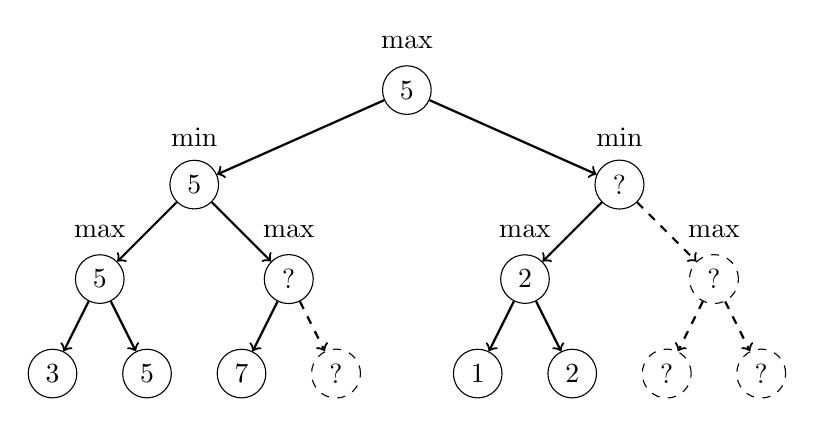
\begin{tikzpicture}[scale=0.6]
\node[draw, circle] (1) at (0,0) {$5$};
\node[draw, circle] (2) at (-4.5,-2) {$5$};
\node[draw, circle] (3) at (4.5,-2) {$?$};
\node[draw, circle] (4) at (-6.5,-4) {$5$};
\node[draw, circle] (5) at (-2.5,-4) {$?$};
\node[draw, circle] (6) at (2.5,-4) {$2$};
\node[draw, circle, dashed] (7) at (6.5,-4) {$?$};
\node[draw, circle] (8) at (-7.5,-6) {$3$};
\node[draw, circle] (9) at (-5.5,-6) {$5$};
\node[draw, circle] (10) at (-3.5,-6) {$7$};
\node[draw, circle, dashed] (11) at (-1.5,-6) {$?$};
\node[draw, circle] (12) at (1.5,-6) {$1$};
\node[draw, circle] (13) at (3.5,-6) {$2$};
\node[draw, circle, dashed] (14) at (5.5,-6) {$?$};
\node[draw, circle, dashed] (15) at (7.5,-6) {$?$};
\path[draw,thick,->] (1) -- (2);
\path[draw,thick,->] (1) -- (3);
\path[draw,thick,->] (2) -- (4);
\path[draw,thick,->] (2) -- (5);
\path[draw,thick,->] (3) -- (6);
\path[draw,thick,->,dashed] (3) -- (7);
\path[draw,thick,->] (4) -- (8);
\path[draw,thick,->] (4) -- (9);
\path[draw,thick,->] (5) -- (10);
\path[draw,thick,->,dashed] (5) -- (11);
\path[draw,thick,->] (6) -- (12);
\path[draw,thick,->] (6) -- (13);
\path[draw,thick,->,dashed] (7) -- (14);
\path[draw,thick,->,dashed] (7) -- (15);
\node at (0,1) {max};
\node at (-4.5,-1) {min};
\node at (4.5,-1) {min};
\node at (-6.5,-3) {max};
\node at (-2.5,-3) {max};
\node at (2.5,-3) {max};
\node at (6.5,-3) {max};
\end{tikzpicture}
\caption{Alfa-beeta-karsinnan vaikutus.}
\label{fig:alfbet}
\end{figure}

\index{alfa-beeta-karsinta}
Minimax-algoritmin toimintaa on mahdollista tehostaa
alfa-beeta-karsinnalla, joka jättää puun osia tutkimatta,
jos on selvää, että ne eivät voi vaikuttaa tekoälyn valintaan.
Tämä muistuttaa aiemmin peruuttavan haun yhteydessä
hyödyntämäämme branch and bound -tekniikaa.

Kuva \ref{fig:alfbet} näyttää, kuinka alfa-beeta-karsinta
onnistuu tehostamaan hakua esimerkkitilanteessamme.
Katkoviivoilla esitetyt puun osat ovat sellaisia,
joita ei ole tarpeen tutkia, koska ne eivät voisi vaikuttaa
ylempänä puussa olevaan osittain laskettuun minimiin tai maksimiin.

Kun tekoäly saapuu vasemmassa haarassa solmuun,
jonka arvona on 7, sen ei enää tarvitse tutkia muita
vasemman haaran solmuja. Tämä johtuu siitä, että tekoäly
tietää jo tässä vaiheessa, että vasemman haaran minimi
on enintään 5. Niinpä sen ei tarvitse laskea maksimia luvusta
7 ja jostain toisesta luvusta, koska tämä ei voisi muuttaa minimiä.

Kun sitten oikeassa haarassa tekoäly on laskenut
toiseksi alimmalla tasolla olevaan solmuun
maksimin 2, sen ei enää tarvitse tutkia muita oikean haaran solmuja.
Tämä johtuu siitä, että juuren maksimi on ainakin 5 ja
oikeassa haarassa valittaisiin minimi luvusta 2 ja jostain toisesta luvusta,
mikä ei voisi kasvattaa juuressa olevaa maksimia.

\chapter{Dynaaminen ohjelmointi}

\index{dynaaminen ohjelmointi}

\emph{Dynaaminen ohjelmointi} (\emph{dynamic programming}) on tekniikka,
jonka avulla voi monessa tilanteessa
laskea ongelman ratkaisujen yhteismäärän tai
löytää ratkaisun, joka on jollain tavalla optimaalinen.
Ideana on muotoilla ongelma rekursiivisesti niin,
että ongelman ratkaisu voidaan muodostaa pienemmistä osaongelmista.
Tämän jälkeen saamme aikaan tehokkaan algoritmin,
kun käsittelemme jokaisen osaongelman vain kerran.

Tässä luvussa tutustumme ensin dynaamisen ohjelmoinnin perusteisiin
toteuttamalla tehokkaan algoritmin, joka laskee palikkayhdistelmien määrän.
Tämän jälkeen käymme läpi kokoelman muita esimerkkejä, jotka esittelevät
lisää dynaamisen ohjelmoinnin mahdollisuuksia.

\section{Perustekniikat}

Aloitamme dynaamiseen ohjelmointiin tutustumisen tehtävästä,
jossa haluamme rakentaa palikoista tornin, jonka korkeus on $n$.
Kunkin palikan korkeus on 1, 2 tai 3,
ja jokaista palikkatyyppiä on saatavilla rajattomasti.
Monellako tavalla voimme rakentaa tornin?

\begin{figure}
\center
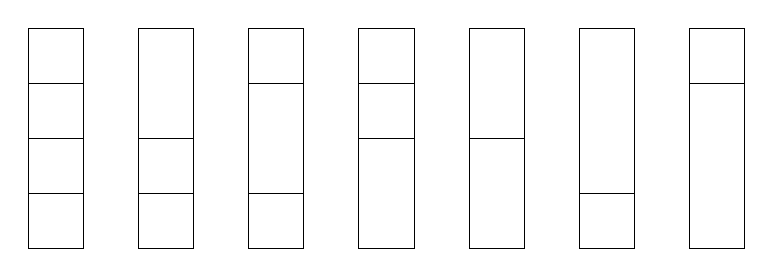
\begin{tikzpicture}[scale=0.7]
\newcommand\palikka[3]{
\draw (2*#1,#2) rectangle (2*#1+1,#2+#3);
}
\palikka{0}{0}{1} \palikka{0}{1}{1} \palikka{0}{2}{1} \palikka{0}{3}{1}
\palikka{1}{0}{1} \palikka{1}{1}{1} \palikka{1}{2}{2}
\palikka{2}{0}{1} \palikka{2}{1}{2} \palikka{2}{3}{1}
\palikka{3}{0}{2} \palikka{3}{2}{1} \palikka{3}{3}{1}
\palikka{4}{0}{2} \palikka{4}{2}{2}
\palikka{5}{0}{1} \palikka{5}{1}{3}
\palikka{6}{0}{3} \palikka{6}{3}{1}
\end{tikzpicture}
\caption{Voimme rakentaa korkeuden 4 tornin 7 tavalla palikoista,
joiden korkeudet ovat 1, 2 ja 3.}
\label{fig:dyntor}
\end{figure}

Esimerkiksi kun tornin korkeus on $n=4$, voimme rakentaa
sen 7 tavalla kuvan \ref{fig:dyntor} mukaisesti.
Jos $n$ on pieni, voimme laskea tornien määrän helposti
käymällä läpi kaikki tavat, mutta tornien määrä kasvaa
nopeasti emmekä voi käyttää raakaa voimaa suuremmilla
$n$:n arvoilla.
Seuraavaksi ratkaisemmekin ongelman tehokkaasti
dynaamisella ohjelmoinnilla.

\subsection{Rekursiivinen esitys}

Jotta voimme käyttää dynaamista ohjelmointia,
ongelma täytyy pystyä esit\-tämään \emph{rekursiivisesti}
niin, että saamme laskettua ongelman ratkaisun
käyt\-täen osaongelmina pienempiä vastaavia ongelmia.
Tässä tehtävässä luonteva rekursiivinen funktio on
$\texttt{tornit}(n)$: monellako tavalla voimme
rakentaa tornin, jonka korkeus on $n$?
Esimerkiksi $\texttt{tornit}(4)=7$, koska
voimme rakentaa korkeuden 4 tornin 7 tavalla.

Funktion pienten arvojen laskeminen on helppoa.
Ensinnäkin $\texttt{tornit}(0)=1$, koska on
tarkalleen yksi tapa rakentaa tyhjä torni:
siinä ei ole mitään palikoita.
Sitten $\texttt{tornit}(1)=1$, koska ainoa tapa
rakentaa korkeuden 1 torni on valita palikka, jonka korkeus on 1,
ja $\texttt{tornit}(2)=2$, koska voimme
rakentaa korkeuden 2 tornin valitsemalla joko
kaksi palikkaa, jonka kummankin korkeus on 1,
tai yhden palikan, jonka korkeus on 2.

\begin{figure}
\center
\begin{tikzpicture}[scale=0.7]
\draw (0,0) rectangle (1,1);
\draw[dashed] (0,1) rectangle (1,4);
\draw (4,0) rectangle (5,2);
\draw[dashed] (4,2) rectangle (5,4);
\draw (8,0) rectangle (9,3);
\draw[dashed] (8,3) rectangle (9,4);
\draw [decorate,decoration={brace,amplitude=4pt},xshift=0.2cm] (1,4) -- (1,1) node [midway,right,xshift=.1cm] {$n-1$};
\draw [decorate,decoration={brace,amplitude=4pt},xshift=0.2cm] (5,4) -- (5,2) node [midway,right,xshift=.1cm] {$n-2$};
\draw [decorate,decoration={brace,amplitude=4pt},xshift=0.2cm] (9,4) -- (9,3) node [midway,right,xshift=.1cm] {$n-3$};
\end{tikzpicture}
\caption{Rekursiivinen idea: kun alamme rakentaa tornia, voimme laittaa pohjalle
korkeuden 1, 2 tai 3 palikan.}
\label{fig:dynrek}
\end{figure}

Kuinka voisimme sitten laskea funktion arvon \emph{yleisessä} tapauksessa,
kun tornin korkeus on $n$?
Tässä voimme miettiä, kuinka tornin rakentaminen alkaa.
Mahdollisuuksia on kolme: voimme laittaa ensin palikan,
jonka korkeus on 1, 2 tai 3.
Jos aloitamme korkeuden 1 palikalla, sen päälle
täytyy rakentaa korkeuden $n-1$ torni.
Vastaavasti jos aloitamme korkeuden 2 tai 3 palikalla,
sen päälle täytyy rakentaa torni,
jonka korkeus on $n-2$ tai $n-3$.
Kuva \ref{fig:dynrek} havainnollistaa tämän idean.
Niinpä voimme laskea tornien määrän rekursiivisesti kaavalla
\[
\texttt{tornit}(n) = \texttt{tornit}(n-1)+\texttt{tornit}(n-2)+\texttt{tornit}(n-3),
\]
kun $n \ge 3$.
Esimerkiksi voimme laskea
\[
\texttt{tornit}(3) = \texttt{tornit}(2)+\texttt{tornit}(1)+\texttt{tornit}(0)=4
\]
ja
\[
\texttt{tornit}(4) = \texttt{tornit}(3)+\texttt{tornit}(2)+\texttt{tornit}(1)=7,
\]
jolloin olemme saaneet laskettua esimerkkitapaustamme vastaavasti,
että voimme rakentaa korkeuden 4 tornin 7 tavalla.

\begin{table}
\center
\begin{tabular}{rrr}
korkeus $n$ & $\texttt{tornit}(n)$ \\
\hline
0 & 1 \\
1 & 1 \\
2 & 2 \\
3 & 4 \\
4 & 7 \\
5 & 13 \\
6 & 24 \\
7 & 44 \\
8 & 81 \\
9 & 149 \\
\end{tabular}
\caption{Tornien määrät, kun korkeus $n$ on $0,1,\dots,9$.}
\label{tab:dyntor}
\end{table}

Taulukko \ref{tab:dyntor} näyttää funktion
$\texttt{tornit}(n)$ arvot, kun $n=0,1,\dots,9$.
Kuten taulukosta voi huomata, funktion arvo kasvaa nopeasti:
se lähes kaksinkertaistuu joka askeleella.
Kun $n$ on suuri,
onkin valtavasti mahdollisuuksia tornin rakentamiseen.

\subsection{Tehokas toteutus}

Nyt kun olemme saaneet aikaan rekursiivisen funktion,
voimme toteuttaa sen ohjelmoimalla seuraavasti:

\begin{code}
function tornit(n)
    if (n == 0) return 1
    if (n == 1) return 1
    if (n == 2) return 2
    return tornit(n-1)+tornit(n-2)+tornit(n-3)
\end{code}

Tämä on toimiva ratkaisu, mutta siinä on yksi ongelma:
funktion arvon laskeminen vie kauan aikaa, jos $n$ on
vähänkin suurempi.
Käytännössä laskenta alkaa hidastua parametrin $n=30$ tienoilla.
Esimerkiksi arvon $\texttt{tornit}(40)$ laskeminen vie aikaa
noin minuutin ja arvon $\texttt{tornit}(50)$ vie aikaa niin kauan,
että emme jaksa odottaa laskennan valmistumista.

Syynä laskennan hitauteen on, että funktiota $\texttt{tornit}$
kutsutaan uudestaan ja uudestaan samoilla parametreilla
ja tornien määrä lasketaan loppujen lopuksi summana
luvuista 1 ja 2 pohjatapauksista.
Niinpä kun tornien määrä on suuri,
laskenta on tuomittu viemään kauan aikaa.
Voimme kuitenkin tehostaa laskentaa toteuttamalla
sen hieman toisella tavalla.

\index{taulukointi}

Tässä astuu kuvaan dynaamisen ohjelmoinnin keskeinen idea
\emph{taulukointi} (\emph{memoization}):
laskemme funktion arvon kullekin parametrille vain kerran
ja tallennamme tulokset taulukkoon myöhempää käyttöä varten.
Tätä varten luomme taulukon $\texttt{tornit}$,
jossa kohtaan $\texttt{tornit}[i]$ tallennetaan funktion
arvo $\texttt{tornit}(i)$.
Kun haluamme laskea korkeuden $n$ tornien määrän,
täytämme taulukon kohdat $0,1,\dots,n$.
Seuraava koodi toteuttaa laskennan:

\begin{code}
tornit[0] = 1
tornit[1] = 1
tornit[2] = 2
for i = 3 to n
    tornit[i] = tornit[i-1]+tornit[i-2]+tornit[i-3]
\end{code}

Koodin suorituksen jälkeen taulukon arvo $\texttt{tornit}[n]$
kertoo, monellako tavalla voimme rakentaa
korkeuden $n$ tornin.

Tämän toteutuksen etuna on, että se on huomattavasti
nopeampi kuin rekursiivinen funktio.
Koska koodissa on vain yksi for-silmukka, se vie aikaa
vain $O(n)$, eli voimme käsitellä tehokkaasti myös
suuria $n$:n arvoja.
Esimerkiksi voimme nyt laskea salamannopeasti, että
\[
\texttt{tornit}(50) = 10562230626642
\]
eli on yli 10562 miljardia tapaa rakentaa korkeuden 50 torni.

\section{Esimerkkejä}

Olemme nyt tutustuneet dynaamisen ohjelmoinnin perusideaan,
mutta tämä on vasta alkua sille, mitä kaikkea tekniikan
avulla pystyy tekemään.
Seuraavaksi käymme läpi kokoelman tehtäviä,
jotka esittelevät lisää dynaamisen ohjelmoinnin mahdollisuuksia.

\subsection{Pisin nouseva alijono}

\index{pisin nouseva alijono}

Ensimmäinen tehtävä on selvittää, kuinka pitkä on
$n$ alkiota sisältävän taulukon \emph{pisin nouseva alijono}
(\emph{longest increasing subsequence}) eli
mahdollisimman pitkä vasemmalta oikealle etenevä jono alkioita,
jossa seuraava alkio on aina edellistä suurempi.
Kuvassa \ref{fig:pisnou} on esimerkki taulukosta,
jonka pisin nouseva alijono $[2,5,7,8]$ on pituudeltaan 4.

\begin{figure}
\center
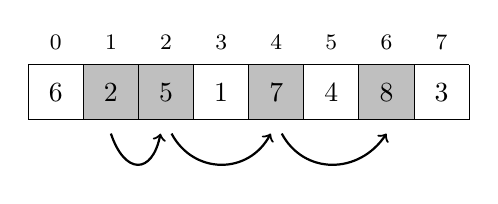
\begin{tikzpicture}[scale=0.7]
\fill[color=lightgray] (1,0) rectangle (2,1);
\fill[color=lightgray] (2,0) rectangle (3,1);
\fill[color=lightgray] (4,0) rectangle (5,1);
\fill[color=lightgray] (6,0) rectangle (7,1);
\draw (0,0) grid (8,1);
\node at (0.5,0.5) {$6$};
\node at (1.5,0.5) {$2$};
\node at (2.5,0.5) {$5$};
\node at (3.5,0.5) {$1$};
\node at (4.5,0.5) {$7$};
\node at (5.5,0.5) {$4$};
\node at (6.5,0.5) {$8$};
\node at (7.5,0.5) {$3$};
\draw[thick,->] (1.5,-0.25) .. controls (1.75,-1.00) and (2.25,-1.00) .. (2.4,-0.25);
\draw[thick,->] (2.6,-0.25) .. controls (3.0,-1.00) and (4.0,-1.00) .. (4.4,-0.25);
\draw[thick,->] (4.6,-0.25) .. controls (5.0,-1.00) and (6.0,-1.00) .. (6.5,-0.25);
\footnotesize
\node at (0.5,1.4) {$0$};
\node at (1.5,1.4) {$1$};
\node at (2.5,1.4) {$2$};
\node at (3.5,1.4) {$3$};
\node at (4.5,1.4) {$4$};
\node at (5.5,1.4) {$5$};
\node at (6.5,1.4) {$6$};
\node at (7.5,1.4) {$7$};
\end{tikzpicture}
\caption{Taulukon pisin nouseva alijono on $[2,5,7,8]$.}
\label{fig:pisnou}
\end{figure}

Voimme lähestyä tehtävää laskemalla jokaiselle taulukon
kohdalle $k=0,1,\dots,n-1$ arvon $\texttt{pisin}(k)$:
kuinka pitkä on pisin nouseva alijono, joka päättyy kohtaan $k$.
Kun olemme laskeneet kaikki nämä arvot, suurin arvoista kertoo meille,
kuinka pitkä on pisin nouseva alijono koko taulukossa.
Esimerkiksi kuvan \ref{fig:pisnou} taulukossa $\texttt{pisin}(6)=4$,
koska kohtaan $6$ päättyvä pisin nouseva alijono on pituudeltaan $4$.

Millainen on sitten pisin kohtaan $k$ päättyvä alijono?
Yksi mahdollisuus on, että alijonossa on vain kohdan $k$ alkio,
jolloin $\texttt{pisin}(k)=1$.
Muussa tapauksessa alijonossa on ensin kohtaan $x$ päättyvä
pisin nouseva alijono, missä $x<k$, ja sitten vielä kohdan $k$ alkio.
Tämä edellyttää, että kohdan $x$ alkio on pienempi
kuin kohdan $k$ alkio.
Tuloksena olevan alijonon pituus on $\texttt{pisin}(x)+1$.
Tämä antaa mahdollisuuden dynaamiseen ohjelmointiin:
kun haluamme laskea arvon $\texttt{pisin}(k)$,
käymme läpi kaikki mahdolliset tavat valita kohta $x$
ja valitsemme niistä parhaan vaihtoehdon.

Seuraava koodi laskee jokaiselle $k=0,1,\dots,n-1$
pisimmän kohtaan $k$ päättyvän alijonon pituuden yllä kuvattua
ideaa käyttäen.
Koodi olettaa, että taulukon sisältö on taulukossa \texttt{taulu},
ja se muodostaa taulukon \texttt{pisin}, jossa on pisimpien
alijonojen pituudet.

\begin{code}
for k = 0 to n-1
    pisin[k] = 1
    for x = 0 to k-1
        if taulu[x] < taulu[k] and pisin[x]+1 > pisin[k]
            pisin[k] = pisin[x]+1
\end{code}

Koodin suorituksen jälkeen pisimmän nousevan alijonon pituus on
siis suurin taulukon \texttt{pisin} arvoista.
Tämä algoritmi vie aikaa $O(n^2)$, koska käym\-me jokaisessa
kohdassa $k$ läpi kaikki taulukon edelliset kohdat.

Mitä jos haluaisimme selvittää pisimmän nousevan alijonon
pituuden lisäksi, mistä alkioista se muodostuu?
Tämä onnistuu laajentamalla hieman koodia.
Rakennamme taulukon \texttt{aiempi},
joka kertoo jokaisessa kohdassa, missä on tähän kohtaan
päättyvän pisimmän alijonon edellinen alkio.
Voimme muodostaa taulukon seuraavasti:

\begin{code}
for k = 0 to n-1
    pisin[k] = 1
    aiempi[k] = -1
    for x = 0 to k-1
        if taulu[x] < taulu[k] and pisin[x]+1 > pisin[k]
            pisin[k] = pisin[x]+1
            aiempi[k] = x
\end{code}

Tämän jälkeen jokaisessa kohdassa $k$ arvo $\texttt{aiempi}[k]$
kertoo pisimmän alijonon edellisen alkion kohdan.
Kuitenkin jos alijonon pituus on 1, taulukossa on arvo $-1$.
Voimme nyt selvittää kohtaan $k$ päättyvän alijonon alkiot
käänteisesti seuraavasti:

\begin{code}
while k != -1
    print(taulu[k])
    k = aiempi[k]
\end{code}

Voimme käyttää vastaavaa tekniikkaa
dynaamisessa ohjelmoinnissa aina, kun haluamme
selvittää, mistä aineksista paras ratkaisu muodostuu.

\subsection{Reitti ruudukossa}

Olemme $n \times n$ -ruudukon vasemmassa yläkulmassa ja haluamme
päästä oikeaan alakulmaan.
Jokaisella vuorolla voimme siirtyä askeleen alaspäin tai oikealle.
Kuitenkin joissakin ruuduissa on este, emmekä voi kulkea sellaisen
ruudun kautta.
Montako mahdollista reittiä on olemassa?
Esimerkiksi kuvassa \ref{fig:reiruu} on $4 \times 4$ -ruudukko,
jossa on kolme mahdollista reittiä ruudukon
vasemmasta yläkulmasta oikeaan alakulmaan.

\begin{figure}
\center
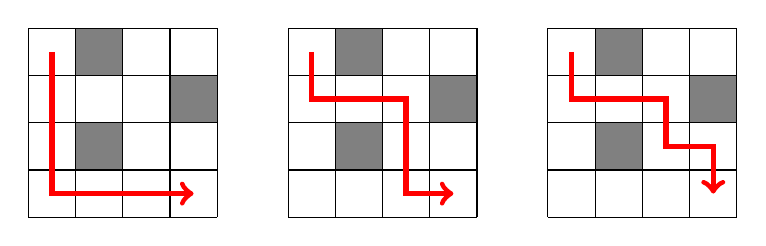
\begin{tikzpicture}[scale=0.6]
\newcommand\ruudukko{
\fill[color=gray] (1,1) rectangle (2,2);
\fill[color=gray] (1,3) rectangle (2,4);
\fill[color=gray] (3,2) rectangle (4,3);
\draw (0,0) grid (4,4);
}
\begin{scope}
\ruudukko
\draw[thick,->,red,line width=2pt] (0.5,3.5) -- (0.5,0.5) -- (3.5,0.5);
\end{scope}
\begin{scope}[xshift=5.5cm]
\ruudukko
\draw[thick,->,red,line width=2pt] (0.5,3.5) -- (0.5,2.5) -- (2.5,2.5) -- (2.5,0.5) -- (3.5,0.5);
\end{scope}
\begin{scope}[xshift=11cm]
\ruudukko
\draw[thick,->,red,line width=2pt] (0.5,3.5) -- (0.5,2.5) -- (2.5,2.5) -- (2.5,1.5) -- (3.5,1.5) -- (3.5,0.5);
\end{scope}
\end{tikzpicture}
\caption{Mahdolliset reitit vasemmasta yläkulmasta oikeaan alakulmaan.}
\label{fig:reiruu}
\end{figure}

Tässä tehtävässä osaongelmat ovat \emph{kaksiulotteisia},
koska olemme reitin joka vaiheessa tietyn rivin tietyssä sarakkeessa.
Niinpä määritte\-lemme rekursiivisen funktion, jolla on kaksi
parametria: $\texttt{reitit}(y,x)$ kertoo, montako reittiä on
vasemmasta yläkulmasta ruutuun $(y,x)$.
Numeroimme rivit ja sarakkeet $1,2,\dots,n$
ja haluamme laskea arvon $\texttt{reitit}(n,n)$,
joka on reittien määrä vasemmasta yläkulmasta oikeaan alakulmaan.

Hyödyllinen havainto on, että jokaisessa ruudussa on kaksi
mahdollisuutta, kuinka reitti voi tulla ruutuun,
koska voimme tulla joko ylhäältä tai vasemmalta.
Kun haluamme laskea reittien määrää, laskemmekin yhteen ylhäältä
ja vasemmalta tulevat reitit.
Rajoituksena jos ruudussa on este, siihen tulevien reittien
määrä on aina nolla.
Tämän perusteella saamme aikaan seuraavan
dynaamisen ohjelmoinnin algoritmin:

\begin{code}
for y = 1 to n
    for x = 1 to n
        if este[y][x]
            reitit[y][x] = 0
        else if y == 1 and x == 1
            reitit[y][x] = 1
        else
            reitit[y][x] = reitit[y-1][x]+reitit[y][x-1]
\end{code}

Koodi laskee jokaiseen ruutuun reittien määrän
vasemmasta yläkulmasta kyseiseen ruutuun.
Jos ruudussa on este, reittien määrä on 0,
koska mitään reittiä ei ole olemassa.
Jos ruutu on vasen yläkulma (eli $y=1$ ja $x=1$),
reittien määrä on 1, koska reitti alkaa siitä ruudusta.
Muuten reittien määrä saadaan laskemalla yhteen
ylhäältä ja vasemmalta tulevat reitit.
Tuloksena on algoritmi, joka vie aikaa $O(n^2)$.

Huomaa, että tässä käytämme taulukon kohtia $1,2,\dots,n$
ja oletamme, että kohdissa $0$ on arvona nolla.
Tämä on kätevää, koska meidän ei tarvitse tehdä erikoistapauksia
ruudukon yläreunaa ja vasenta reunaa varten.

\subsection{Repunpakkaus}

\index{repunpakkaus}

Termi \emph{repunpakkaus} (\emph{knapsack}) viittaa ongelmaan,
jossa halutaan selvittää, millaisia yhdistelmiä voidaan muodostaa tavaroista,
joilla on tietyt painot.
Ongelmasta on monia muunnelmia, joiden yhdistävänä tekijänä on,
että ne voi ratkaista tehokkaasti dynaamisella ohjelmoinnilla.

Seuraavaksi keskitymme ongelmaan, jossa meillä on $n$ tavaraa,
joilla on painot $p_1,p_2,\dots,p_n$.
Haluamme selvittää kaikki mahdolliset yhteispainot,
jotka voimme muodostaa valitsemalla jonkin osajoukon tavaroista.
Esimerkiksi jos tavaroiden painot ovat $[1,3,3,4]$,
niin mahdolliset yhteispainot ovat
\[[0,1,3,4,5,6,7,8,10,11].\]
Esimerkiksi yhteispaino $6$ on listalla,
koska saamme sen painoista $3+3=6$,
ja yhteispaino $8$ on listalla,
koska saamme sen painoista $1+3+4=8$.

On helppoa laskea, mikä on suurin mahdollinen tavaroiden yhteispaino,
koska saamme sen valitsemalla kaikki tavarat.
Suurin yhteispaino on siis
\[s=p_1+p_2+\dots+p_n.\]
Tämä on meille hyödyllinen yläraja, koska tiedämme nyt,
että tavaroiden yhteispaino on aina jokin luku välillä $0 \dots s$.

Voimme lähestyä tehtävää dynaamisella ohjelmoinnilla luomalla
funktion $\texttt{painot}(k)$: mitkä kaikki yhteispainot voimme
muodostaa, jos käytös\-sämme on tavarat $1,2,\dots,k$?
Oletamme, että funktio palauttaa \emph{taulukon}, jossa on $s+1$ alkiota:
jokaiselle yhteispainolle $0,1,\dots,s$ tieto siitä,
voimmeko muodostaa sen painoista $p_1,p_2,\dots,p_k$.
Tapaus $\texttt{painot}(0)$ on helppo,
koska kun ei ole mitään tavaroita,
ainoa mahdollinen yhteispaino on $0$.
Tämän jälkeen pystymme laskemaan tapauksen $\texttt{painot}(k)$
ottamalla lähtökohdaksi tapauksen $\texttt{painot}(k-1)$
ja selvittämällä, mitä uusia yhteispainoja voimme muodostaa,
kun saamme käyttää myös painoa $p_k$.

\begin{figure}
\center
\begin{tikzpicture}[scale=0.5]
\draw (0,0) grid (12,5);
\foreach \x in {0,1,...,11} \node at (\x+0.5,5.5) {\x};
\foreach \y in {0,1,2,3,4} \node at (-1.5,4.5-\y) {$k=\y$};
\foreach \x in {0} \node at (\x+0.5,4.5) {\checkmark};
\foreach \x in {0,1} \node at (\x+0.5,3.5) {\checkmark};
\foreach \x in {0,1,3,4} \node at (\x+0.5,2.5) {\checkmark};
\foreach \x in {0,1,3,4,6,7} \node at (\x+0.5,1.5) {\checkmark};
\foreach \x in {0,1,3,4,5,6,7,8,10,11} \node at (\x+0.5,0.5) {\checkmark};
\end{tikzpicture}
\caption{Mahdolliset yhteispainot, kun painot ovat $[1,3,3,4]$.}
\label{fig:reppak}
\end{figure}

Kuva \ref{fig:reppak} näyttää dynaamisen ohjelmoinnin
taulukoiden sisällön esimerkissämme, jossa painot ovat $[1,3,3,4]$.
Ensimmäisellä rivillä $k=0$, joten ainoa yhteispaino on $0$.
Toisella rivillä $k=1$, joten saamme käyttää painoa $p_1=1$
ja voimme muodostaa yhteispainot $0$ ja $1$.
Kolmannella rivillä $k=2$, jolloin saamme käyttöömme painon $p_2=3$
ja voimme muodostaa yhteispainot $0$, $1$, $3$ ja $4$.
Viimeisellä rivillä käytössämme ovat kaikki painot,
joten se vastaa ongelman ratkaisua.

Voimme toteuttaa dynaamisen ohjelmoinnin kätevästi niin,
että koodissa on vain yksi boolean-taulukko \texttt{painot},
jossa on $s+1$ alkiota.
Taulukko kertoo laskennan jokaisessa vaiheessa,
mitkä yhteispainot ovat mahdollisia sillä hetkellä.
Aluksi taulukon kohdassa $0$ on arvo \texttt{true} ja
kaikissa muissa kohdissa on arvo \texttt{false}.
Tämän jälkeen päivitämme taulukkoa lisäämällä mukaan
painoja yksi kerrallaan.

\begin{code}
painot[0] = true
for i = 1 to n
    for j = s to 0
        if painot[j]
            painot[j+p[i]] = true
\end{code}

Tärkeä yksityiskohta algoritmissa on,
että käymme jokaisen painon kohdalla taulukon
läpi \emph{lopusta alkuun}.
Syynä tähän on, että tällä tavalla saamme
laskettua oikealla tavalla, mitä uusia yhteispainoja
voidaan muodostaa, kun saamme käyttää uutta painoa kerran.
Laskennan jälkeen voimme tulostaa kaikki
mahdolliset yhteispainot näin:

\begin{code}
for i = 0 to s
    if painot[i]
        print(i)
\end{code}

Tuloksena olevan algoritmin aikavaativuus on $O(ns)$.
Algoritmin tehokkuus riippuu siis paitsi tavaroiden määrästä,
myös niiden painoista.
Jotta algoritmi on käyttökelpoinen, painojen summan $s$
täytyy olla niin pieni, että voimme varata niin suuren taulukon.

\subsection{Binomikertoimet}

\index{binomikerroin}

\emph{Binomikerroin} $\binom{n}{k}$ ilmaisee, monellako tavalla voimme
muodostaa $n$ alkion joukosta $k$ alkion osajoukon.
Esimerkiksi $\binom{5}{3}=10$, koska voimme muodostaa
joukosta $\{1,2,3,4,5\}$ seuraavat 3 alkion osajoukot:

\begin{multicols}{3}
\begin{itemize}
\item $\{1,2,3\}$
\item $\{1,2,4\}$
\item $\{1,2,5\}$
\item $\{1,3,4\}$
\item $\{1,3,5\}$
\item $\{1,4,5\}$
\item $\{2,3,4\}$
\item $\{2,3,5\}$
\item $\{2,4,5\}$
\item $\{3,4,5\}$
\end{itemize}
\end{multicols}

Binomikertoimien laskemiseen on monia tapoja.
Dynaamisen ohjelmoinnin kannalta kiinnostava tapa on rekursiivinen kaava
\[\binom{n}{k} = \binom{n-1}{k-1} + \binom{n-1}{k}.\]
Voimme perustella kaavan tarkastelemalla
$k$ alkion osajoukon muodostamista joukosta $\{1,2,\dots,n\}$.
Jos otamme osajoukkoon mukaan alkion $n$, tämän jälkeen tulee muodostaa
vielä $k-1$ alkion osajoukko joukosta $\{1,2,\dots,n-1\}$.
Jos taas emme ota osajoukkoon mukaan alkiota $n$, tämän jälkeen tulee muodostaa
$k$ alkion osajoukko joukosta $\{1,2,\dots,n-1\}$.

Lisäksi pohjatapauksina
\[ \binom{n}{0} = 1,\]
koska voimme muodostaa tyhjän osajoukon yhdellä tavalla, ja
\[ \binom{n}{k} = 0,\,\textrm{jos $k>n$},\]
koska $n$ alkiosta ei voi muodostaa osajoukkoa, jossa on yli $n$ alkiota.

Tämä rekursiivinen kaava tarjoaa meille tavan laskea tehokkaasti
binomikertoimia dynaamisen ohjelmoinnin avulla.
Voimme toteuttaa laskennan seuraavasti:

\begin{code}
binom[0][0] = 1
for i = 1 to n
    binom[i][0] = 1
    for j = 1 to k
        binom[i][j] = binom[i-1][j-1]+binom[i-1][j]
\end{code}

Koodin suorituksen jälkeen taulukon kohdassa
$\texttt{binom}[n][k]$ on binomikerroin $\binom{n}{k}$.
Algoritmi vie aikaa $O(nk)$, joten sitä voi käyttää
melko suurten binomikertoimien laskemiseen.

\chapter{Verkkojen perusteet}

\index{verkko}

Voimme ratkaista monia algoritmiikan ongelmia
esittämällä tilanteen \emph{verkkona} (\emph{graph}) ja käyttämällä sitten
sopivaa verkkoalgoritmia.
Tyypillinen esimerkki verkosta on tieverkosto,
joka muodostuu kaupungeista ja niiden välisistä teistä.
Tällaisessa verkossa ongelmana voi olla selvittää vaikkapa,
kuinka voimme matkustaa kaupungista $a$ kaupunkiin $b$.

Tässä luvussa aloitamme verkkoihin tutustumisen
käymällä läpi verkkojen käsitteitä sekä tapoja
esittää verkkoja ohjelmoinnissa.
Tämän jälkeen näemme, miten voimme tutkia verkkojen rakennetta
ja ominaisuuksia syvyyshaun ja leveyshaun avulla.
Seuraavissa kirjan luvuissa jatkamme verkkojen käsittelyä ja
opimme lisää verkkoalgoritmeja.

\section{Verkkojen käsitteitä}

\index{solmu}
\index{kaari}

Verkko muodostuu \emph{solmuista} (\emph{node} tai \emph{vertex}) ja
niiden välisistä \emph{kaarista} (\emph{edge}).
Kuvassa \ref{fig:veresi} on verkko,
jossa on viisi solmua ja seitsemän kaarta.
Merkitsemme verkon solmujen
määrää kirjaimella $n$ ja kaarten määrää
kirjaimella $m$.
Lisäksi numeroimme verkon solmut kokonaisluvuin
$1,2,\dots,n$.

\begin{figure}
\center
\begin{center}
\begin{tikzpicture}[scale=0.6]
\small
\node[draw, circle] (1) at (1,3) {$1$};
\node[draw, circle] (2) at (4,3) {$2$};
\node[draw, circle] (3) at (1,1) {$3$};
\node[draw, circle] (4) at (4,1) {$4$};
\node[draw, circle] (5) at (6,2) {$5$};

\path[draw,thick,-] (1) -- (2);
\path[draw,thick,-] (1) -- (3);
\path[draw,thick,-] (1) -- (4);
\path[draw,thick,-] (3) -- (4);
\path[draw,thick,-] (2) -- (4);
\path[draw,thick,-] (2) -- (5);
\path[draw,thick,-] (4) -- (5);
\end{tikzpicture}
\end{center}
\caption{Verkko, jossa on viisi solmua ja seitsemän kaarta.}
\label{fig:veresi}
\end{figure}

\index{naapuri}
\index{aste}

Kaksi solmua ovat \emph{vierekkäin} (\emph{adjacent}),
jos niiden välillä on kaari.
Solmun \emph{naapureja} (\emph{neighbor}) ovat kaikki solmut,
joihin se on yhteydessä kaarella,
ja solmun \emph{aste} (\emph{degree}) on sen naapureiden määrä.
Kuvassa \ref{fig:veresi} solmun 2 naapurit ovat 1, 4 ja 5,
joten solmun aste on 3.

\subsubsection{Polku ja sykli}

\begin{figure}
\center
\begin{center}
\begin{tikzpicture}[scale=0.6]
\small
\begin{scope}
\node[draw, circle] (1) at (1,3) {$1$};
\node[draw, circle] (2) at (4,3) {$2$};
\node[draw, circle] (3) at (1,1) {$3$};
\node[draw, circle] (4) at (4,1) {$4$};
\node[draw, circle] (5) at (6,2) {$5$};

\path[draw,thick,-] (1) -- (2);
\path[draw,thick,-] (1) -- (3);
\path[draw,thick,-] (1) -- (4);
\path[draw,thick,-] (3) -- (4);
\path[draw,thick,-] (2) -- (4);
\path[draw,thick,-] (2) -- (5);
\path[draw,thick,-] (4) -- (5);

\path[draw,thick,->,red,line width=2pt] (1) -- (2);
\path[draw,thick,->,red,line width=2pt] (2) -- (5);
\end{scope}
\begin{scope}[xshift=8cm]
\node[draw, circle] (1) at (1,3) {$1$};
\node[draw, circle] (2) at (4,3) {$2$};
\node[draw, circle] (3) at (1,1) {$3$};
\node[draw, circle] (4) at (4,1) {$4$};
\node[draw, circle] (5) at (6,2) {$5$};

\path[draw,thick,-] (1) -- (2);
\path[draw,thick,-] (1) -- (3);
\path[draw,thick,-] (1) -- (4);
\path[draw,thick,-] (3) -- (4);
\path[draw,thick,-] (2) -- (4);
\path[draw,thick,-] (2) -- (5);
\path[draw,thick,-] (4) -- (5);

\path[draw,thick,->,red,line width=2pt] (1) -- (3);
\path[draw,thick,->,red,line width=2pt] (3) -- (4);
\path[draw,thick,->,red,line width=2pt] (4) -- (5);
\end{scope}
\end{tikzpicture}
\end{center}
\caption{Kaksi polkua solmusta $1$ solmuun $5$.}
\label{fig:verpoe}
\end{figure}

\index{polku}

Verkossa oleva \emph{polku} (\emph{path}) on kaaria pitkin kulkeva reitti
lähtösolmusta kohdesolmuun.
Kuva \ref{fig:verpoe} näyttää kaksi
mahdollista polkua solmusta $1$ solmuun $5$.
Polut ovat $1 \rightarrow 2 \rightarrow 5$
ja $1 \rightarrow 3 \rightarrow 4 \rightarrow 5$.

\begin{figure}
\center
\begin{center}
\begin{tikzpicture}[scale=0.6]
\small
\node[draw, circle] (1) at (1,3) {$1$};
\node[draw, circle] (2) at (4,3) {$2$};
\node[draw, circle] (3) at (1,1) {$3$};
\node[draw, circle] (4) at (4,1) {$4$};
\node[draw, circle] (5) at (6,2) {$5$};

\path[draw,thick,-] (1) -- (2);
\path[draw,thick,-] (1) -- (3);
\path[draw,thick,-] (1) -- (4);
\path[draw,thick,-] (3) -- (4);
\path[draw,thick,-] (2) -- (4);
\path[draw,thick,-] (2) -- (5);
\path[draw,thick,-] (4) -- (5);

\path[draw,thick,->,red,line width=2pt] (2) -- (4);
\path[draw,thick,->,red,line width=2pt] (4) -- (5);
\path[draw,thick,->,red,line width=2pt] (5) -- (2);
\end{tikzpicture}
\end{center}
\caption{Verkossa on sykli $2 \rightarrow 4 \rightarrow 5 \rightarrow 2$.}
\label{fig:versyk}
\end{figure}

\index{sykli}
\index{syklitön verkko}

Polku on \emph{sykli} (\emph{cycle}), jos sen alku- ja loppusolmu on sama,
siinä on ainakin yksi kaari 
eikä se kulje kahta kertaa saman solmun tai kaaren kautta.
Kuvassa \ref{fig:versyk} on esimerkkinä sykli
$2 \rightarrow 4 \rightarrow 5 \rightarrow 2$.
Jos verkossa ei ole yhtään sykliä, verkko on \emph{syklitön}
(\emph{acyclic}).

\subsubsection{Yhtenäisyys ja komponentit}

\index{yhtenäinen verkko}

Verkko on \emph{yhtenäinen} (\emph{connected}),
jos minkä tahansa kahden solmun välillä on polku.
Kuvan \ref{fig:veresi} verkko on yhtenäinen,
mutta kuvan \ref{fig:veryht} verkko ei ole yhtenäinen,
koska esimerkiksi solmujen $1$ ja $2$ välillä ei ole polkua.

\index{komponentti}
\index{yhtenäinen komponentti}

Verkko voidaan esittää aina kokoelmana yhtenäisiä \emph{komponentteja}
(\emph{component}).
Kuvassa \ref{fig:veryht} yhtenäiset komponentit
ovat $\{1,3\}$ ja $\{2,4,5\}$.

\begin{figure}
\center
\begin{center}
\begin{tikzpicture}[scale=0.6]
\small
\node[draw, circle] (1) at (1,3) {$1$};
\node[draw, circle] (2) at (4,3) {$2$};
\node[draw, circle] (3) at (1,1) {$3$};
\node[draw, circle] (4) at (4,1) {$4$};
\node[draw, circle] (5) at (6,2) {$5$};

\path[draw,thick,-] (1) -- (3);
\path[draw,thick,-] (2) -- (4);
\path[draw,thick,-] (2) -- (5);
\path[draw,thick,-] (4) -- (5);
\end{tikzpicture}
\end{center}
\caption{Verkon yhtenäiset komponentit ovat $\{1,3\}$ ja $\{2,4,5\}$.}
\label{fig:veryht}
\end{figure}

\index{puu}

Verkko on \emph{puu} (\emph{tree}), jos se on sekä yhtenäinen
että syklitön.
Puussa kaarten määrä on aina yhden pienempi
kuin solmujen määrä, ja jokaisen kahden solmun
välillä on yksikäsitteinen polku.
Kuvassa \ref{fig:verpuu} on esimerkkinä puu,
jossa on viisi solmua ja neljä kaarta.

\begin{figure}
\center
\begin{center}
\begin{tikzpicture}[scale=0.6]
\small
\node[draw, circle] (1) at (1,3) {$1$};
\node[draw, circle] (2) at (4,3) {$2$};
\node[draw, circle] (3) at (1,1) {$3$};
\node[draw, circle] (4) at (4,1) {$4$};
\node[draw, circle] (5) at (6,2) {$5$};

\path[draw,thick,-] (1) -- (3);
\path[draw,thick,-] (3) -- (4);
\path[draw,thick,-] (2) -- (4);
\path[draw,thick,-] (4) -- (5);
\end{tikzpicture}
\end{center}
\caption{Puu eli yhtenäinen, syklitön verkko.}
\label{fig:verpuu}
\end{figure}

\subsubsection{Suunnattu verkko}

\index{suunnattu verkko}

Kun verkko on \emph{suunnattu} (\emph{directed}),
jokaisella kaarella on tietty suunta,
jonka mukaisesti kaarta pitkin tulee kulkea.
Suunnat rajoittavat siis verkossa liikkumista.
Kuvassa \ref{fig:versuu} on esimerkkinä
suunnattu verkko, jossa
voimme kulkea solmusta $1$ solmuun $5$
polkua $1 \rightarrow 2 \rightarrow 5$,
mutta emme voi kulkea mitenkään solmusta $5$ solmuun $1$.

\subsubsection{Painotettu verkko}

\index{painotettu verkko}

Kun verkko on \emph{painotettu} (\emph{weighted}),
jokaiseen kaareen liittyy jokin paino,
joka kuvaa tyypillisesti kaaren pituutta.
Kun kuljemme polkua painotetussa verkossa,
polun pituus on kaarten painojen summa.
Kuvassa \ref{fig:verpae} on esimerkkinä painotettu verkko,
jossa polun $1 \rightarrow 2 \rightarrow 5$
pituus on $5+8=13$ ja polun
$1 \rightarrow 3 \rightarrow 4 \rightarrow 5$
pituus on $2+4+3=9$.

\begin{figure}[h]
\center
\begin{center}
\begin{tikzpicture}[scale=0.6]
\small
\node[draw, circle] (1) at (1,3) {$1$};
\node[draw, circle] (2) at (4,3) {$2$};
\node[draw, circle] (3) at (1,1) {$3$};
\node[draw, circle] (4) at (4,1) {$4$};
\node[draw, circle] (5) at (6,2) {$5$};

\path[draw,thick,->] (1) -- (2);
\path[draw,thick,->] (1) -- (3);
\path[draw,thick,->] (1) -- (4);
\path[draw,thick,->] (3) -- (4);
\path[draw,thick,->] (2) -- (4);
\path[draw,thick,->] (2) -- (5);
\path[draw,thick,->] (4) -- (5);
\end{tikzpicture}
\end{center}
\caption{Suunnattu verkko.}
\label{fig:versuu}
\end{figure}

\begin{figure}[h]
\center
\begin{center}
\begin{tikzpicture}[scale=0.6,label distance=-1.5mm]
\small
\node[draw, circle] (1) at (1,3) {$1$};
\node[draw, circle] (2) at (4,3) {$2$};
\node[draw, circle] (3) at (1,1) {$3$};
\node[draw, circle] (4) at (4,1) {$4$};
\node[draw, circle] (5) at (6,2) {$5$};

\path[draw,thick,-] (1) -- node[font=\small,label=above:5] {} (2);
\path[draw,thick,-] (1) -- node[font=\small,label=left:2] {} (3);
\path[draw,thick,-] (1) -- node[font=\small,label=above:9] {} (4);
\path[draw,thick,-] (3) -- node[font=\small,label=below:4] {} (4);
\path[draw,thick,-] (2) -- node[font=\small,label=above:8] {} (5);
\path[draw,thick,-] (4) -- node[font=\small,label=right:2] {} (2);
\path[draw,thick,-] (4) -- node[font=\small,label=below:3] {} (5);
\end{tikzpicture}
\end{center}
\caption{Painotettu verkko.}
\label{fig:verpae}
\end{figure}

\subsubsection{Yksinkertainen verkko}

\index{yksinkertainen verkko}

Usein oletuksena on, että verkko on \emph{yksinkertainen} (\emph{simple}),
jolloin siinä ei ole kahta samanlaista kaarta ja jokainen kaari yhdistää
kaksi eri solmua. Kaikki tähän mennessä kirjassa esitetyt verkot ovat
olleet yksinkertaisia.

Kuvassa \ref{fig:vereiy} on esimerkkinä verkko, joka ei ole yksinkertainen.
Tähän on kaksi syytä: solmujen $1$ ja $2$ välillä on kaksi kaarta
ja lisäksi solmusta $5$ on kaari itseensä.

\begin{figure}
\center
\begin{center}
\begin{tikzpicture}[scale=0.6]
\small
\node[draw, circle] (1) at (1,3) {$1$};
\node[draw, circle] (2) at (4,3) {$2$};
\node[draw, circle] (3) at (1,1) {$3$};
\node[draw, circle] (4) at (4,1) {$4$};
\node[draw, circle] (5) at (6,2) {$5$};

\path[draw,thick,-] (1) edge [bend right=30] (2);
\path[draw,thick,-] (2) edge [bend right=30] (1);
\path[draw,thick,-] (1) -- (3);
\path[draw,thick,-] (3) -- (4);
\path[draw,thick,-] (2) -- (4);
\path[draw,thick,-] (4) -- (5);
%\path[every node/.style={}] (5) edge[loop] (5);

\path[-,every loop/.style={looseness=6}] (5)
         edge [in=120,out=60,loop] ();

\end{tikzpicture}
\end{center}
\caption{Verkko, joka ei ole yksinkertainen.}
\label{fig:vereiy}
\end{figure}

\section{Verkot ohjelmoinnissa}

Verkon esittämiseen ohjelmoinnissa on monia mahdollisuuksia.
Sopivan esitystavan valintaan vaikuttaa,
miten haluamme käsitellä verkkoa algoritmissa,
koska jokaisessa esitystavassa on omat etunsa.
Seuraavaksi käymme läpi kolme tavallista esitystapaa.

\begin{figure}[h]
\center
\begin{center}
\begin{tikzpicture}[scale=0.6]
\small
\begin{scope}
\node[draw, circle] (1) at (1,3) {$1$};
\node[draw, circle] (2) at (4,3) {$2$};
\node[draw, circle] (3) at (1,1) {$3$};
\node[draw, circle] (4) at (4,1) {$4$};
\node[draw, circle] (5) at (6,2) {$5$};

\path[draw,thick,->] (1) -- (2);
\path[draw,thick,->] (1) -- (3);
\path[draw,thick,->] (1) -- (4);
\path[draw,thick,->] (3) -- (4);
\path[draw,thick,->] (2) -- (4);
\path[draw,thick,->] (2) -- (5);
\path[draw,thick,->] (4) -- (5);
\end{scope}
\begin{scope}[xshift=9cm,yshift=-0.5cm]
\draw (0,0) grid (1,5);
\foreach \x in {1,...,5} \node at (0.5,0.5-\x+5) {\x};
\draw[->,thick] (1,4.5) -- (2,4.5);
\draw[->,thick] (1,3.5) -- (2,3.5);
\draw[->,thick] (1,2.5) -- (2,2.5);
\draw[->,thick] (1,1.5) -- (2,1.5);
\draw (2,4.1) rectangle (2.8,4.9);
\draw (2.8,4.1) rectangle (3.6,4.9);
\draw (3.6,4.1) rectangle (4.4,4.9);
\draw (2,3.1) rectangle (2.8,3.9);
\draw (2.8,3.1) rectangle (3.6,3.9);
\draw (2,2.1) rectangle (2.8,2.9);
\draw (2,1.1) rectangle (2.8,1.9);
\node at (2.4,4.5) {$2$};
\node at (3.2,4.5) {$3$};
\node at (4.0,4.5) {$4$};
\node at (2.4,3.5) {$4$};
\node at (3.2,3.5) {$5$};
\node at (2.4,2.5) {$4$};
\node at (2.4,1.5) {$5$};
\end{scope}
\end{tikzpicture}
\end{center}
\caption{Verkon vieruslistaesitys.}
\label{fig:vervil}
\end{figure}

\subsection{Vieruslistaesitys}

\index{vieruslista}

Tavallisin tapa esittää verkko on luoda kullekin solmulle
\emph{vieruslista} (\emph{adjacency list}), joka kertoo, mihin solmuihin voimme
siirtyä solmusta kaaria pitkin.
Kuvassa \ref{fig:vervil} on esimerkkinä verkko
ja sitä vastaava vieruslistaesitys.
Voimme luoda vieruslistat näin ohjelmoinnissa:

\begin{code}
verkko[1].add(2)
verkko[1].add(3)
verkko[1].add(4)
verkko[2].add(4)
verkko[2].add(5)
verkko[3].add(4)
verkko[4].add(5)
\end{code}

Vieruslistaesitys on monessa tilanteessa hyvä tapa tallentaa verkko,
koska haluamme usein selvittää,
mihin solmuihin pääsemme siirtymään tietystä solmusta kaaria pitkin.
Esimerkiksi seuraava koodi käy läpi solmut,
joihin voimme siirtyä solmusta $a$ kaarella:

\begin{code}
for b in verkko[a]
    // käsittele solmu b
\end{code}

Suuntaamaton verkko voidaan esittää vieruslistoina niin,
että jokainen kaari tallennetaan molempiin suuntiin.
Jos taas verkko on painotettu, voimme tallentaa jokaisesta
kaaresta sekä kohdesolmun että painon.

\subsection{Kaarilistaesitys}

\index{kaarilista}

Toinen tapa tallentaa verkko on luoda \emph{kaarilista}
(\emph{edge list}),
joka sisältää kaikki verkon kaaret.
Voisimme luoda esimerkkiverkon kaarilistan näin:

\begin{code}
kaaret.add((1,2))
kaaret.add((1,3))
kaaret.add((1,4))
kaaret.add((2,4))
kaaret.add((2,5))
kaaret.add((3,4))
kaaret.add((4,5))
\end{code}

Tässä tapauksessa jokainen listan alkio on pari,
jossa on kaaren alku- ja loppusolmu.
Vastaavasti voisimme tallentaa myös kaaret kolmikkoina,
joissa on lisäksi mukana kaaren paino.

Kaarilista on hyvä esitystapa algoritmeissa,
joissa tulee pystyä käy\-mään helposti läpi
kaikki verkon kaaret eikä ole tarvetta
selvittää tietystä solmusta lähteviä kaaria.

\subsection{Vierusmatriisiesitys}

\begin{figure}
\center
\begin{center}
\begin{tikzpicture}[scale=0.6]
\small
\begin{scope}
\node[draw, circle] (1) at (1,3) {$1$};
\node[draw, circle] (2) at (4,3) {$2$};
\node[draw, circle] (3) at (1,1) {$3$};
\node[draw, circle] (4) at (4,1) {$4$};
\node[draw, circle] (5) at (6,2) {$5$};

\path[draw,thick,->] (1) -- (2);
\path[draw,thick,->] (1) -- (3);
\path[draw,thick,->] (1) -- (4);
\path[draw,thick,->] (3) -- (4);
\path[draw,thick,->] (2) -- (4);
\path[draw,thick,->] (2) -- (5);
\path[draw,thick,->] (4) -- (5);
\end{scope}
\begin{scope}[xshift=9cm,yshift=-0.5cm]
\draw (0,0) grid (5,5);
\foreach \x in {1,...,5} \node at (-0.5,0.5-\x+5) {\x};
\foreach \x in {1,...,5} \node at (-0.5+\x,5.5) {\x};
\foreach \x/\v in {1/0,2/1,3/1,4/1,5/0} \node at (-0.5+\x,4.5) {\v};
\foreach \x/\v in {1/0,2/0,3/0,4/1,5/1} \node at (-0.5+\x,3.5) {\v};
\foreach \x/\v in {1/0,2/0,3/0,4/1,5/0} \node at (-0.5+\x,2.5) {\v};
\foreach \x/\v in {1/0,2/0,3/0,4/0,5/1} \node at (-0.5+\x,1.5) {\v};
\foreach \x/\v in {1/0,2/0,3/0,4/0,5/0} \node at (-0.5+\x,0.5) {\v};
\end{scope}
\end{tikzpicture}
\end{center}
\caption{Verkon vierusmatriisiesitys.}
\label{fig:vervim}
\end{figure}

\index{vierusmatriisi}

\emph{Vierusmatriisi} (\emph{adjacency matrix}) on kaksiulotteinen rakenne,
joka kertoo jokaisesta verkon kaaresta,
esiintyykö se verkossa.
Matriisin rivin $a$ sarakkeessa $b$ oleva arvo
ilmaisee, onko verkossa kaarta solmusta $a$ solmuun $b$.
Kuvassa \ref{fig:vervim} on esimerkki
verkon vierusmatriisiesityksestä.
Tässä tapauksessa matriisin jokainen arvo on
0 (ei kaarta) tai 1 (kaari).

Ohjelmoinnissa voimme tallentaa vierusmatriisin kaksiulotteisena
taulukkona tai listana. Tässä on esimerkkiverkkoa vastaava
vierusmatriisi:

\begin{code}
verkko[1][2] = 1
verkko[1][3] = 1
verkko[1][4] = 1
verkko[2][4] = 1
verkko[2][5] = 1
verkko[3][4] = 1
verkko[4][5] = 1
\end{code}

Jos verkko on painotettu, kaarten painot voidaan vastaavasti
merkitä vierusmatriisiin.
Vierusmatriisin etuna on, että siitä voi tarkastaa helposti,
onko tietty kaari verkossa.
Esitystapa kuluttaa kuitenkin paljon muistia,
eikä sitä voi käyttää, jos verkon solmujen määrä on suuri.

\section{Verkon läpikäynti}

Tutustumme seuraavaksi kahteen keskeiseen verkkoalgoritmiin,
jotka käyvät läpi verkossa olevia solmuja ja kaaria.
Ensin käsittelemme syvyyshakua, joka on yleiskäyttöinen algoritmi
verkon läpikäyntiin, ja sen jälkeen leveyshakua,
jonka avulla voimme löytää lyhimpiä polkuja verkossa.

\subsection{Syvyyshaku}

\index{syvyyshaku}

\emph{Syvyyshaku} (\emph{depth-first search} eli \emph{DFS})
on verkkojen käsittelyn yleistyökalu,
jonka avulla voimme selvittää monia asioita verkon rakenteesta.
Kun alamme tutkia verkkoa syvyyshaulla,
tulee päättää ensin, mistä solmusta haku lähtee liikkeelle.
Haku etenee vuorollaan kaikkiin solmuihin, jotka ovat saavutettavissa
lähtösolmusta kulkemalla kaaria pitkin.

Syvyyshaku pitää yllä jokaisesta verkon solmusta tietoa,
onko solmussa jo vierailtu.
Kun haku saapuu solmuun, jossa se ei ole vieraillut aiemmin,
se merkitsee solmun vierailluksi ja alkaa käydä
läpi solmusta lähteviä kaaria.
Jokaisen kaaren kohdalla haku etenee verkon niihin osiin,
joihin pääsee kaaren kautta.
Lopulta kun haku on käynyt läpi kaikki kaaret,
se perääntyy taaksepäin samaa reittiä kuin tuli solmuun.

Kuvassa \ref{fig:syvhak} on esimerkki syvyyshaun toiminnasta.
Jokaisessa vaiheessa harmaat solmut ovat solmuja,
joissa haku on jo vieraillut.
Tässä esimerkissä haku lähtee liikkeelle solmusta 1,
josta pääsee kaarella solmuihin 2 ja 3.
Haku etenee ensin solmuun 2, josta pääsee edelleen
solmuihin 4 ja 5.
Tämän jälkeen haku ei enää löydä uusia solmuja
tästä verkon osasta, joten se perääntyy takaisin
kulkemaansa reittiä solmuun 1.
Lopuksi haku käy vielä solmussa 3,
josta ei pääse muihin uusiin solmuihin.
Nyt haku on käynyt läpi kaikki solmut,
joihin pääsee solmusta 1.

\begin{figure}
\center
\begin{center}
\begin{tikzpicture}[scale=0.6]
\scriptsize
\newcommand\verkko[6]{
\node[draw, circle, fill=#2] (1) at (0,0) {$1$};
\node[draw, circle, fill=#3] (2) at (2,0) {$2$};
\node[draw, circle, fill=#4] (3) at (0,-2) {$3$};
\node[draw, circle, fill=#5] (4) at (2,-2) {$4$};
\node[draw, circle, fill=#6] (5) at (4,-1) {$5$};
\path[draw,thick,-] (1) -- (2);
\path[draw,thick,-] (2) -- (5);
\path[draw,thick,-] (2) -- (4);
\path[draw,thick,-] (4) -- (5);
\path[draw,thick,-] (1) -- (3);
\node at (2,-3) {vaihe #1};
}
\begin{scope}
\verkko{1}{lightgray}{white}{white}{white}{white}
\end{scope}
\begin{scope}[xshift=6cm]
\verkko{2}{lightgray}{lightgray}{white}{white}{white}
\path[draw=red,thick,->,line width=2pt] (1) -- (2);
\end{scope}
\begin{scope}[xshift=12cm]
\verkko{3}{lightgray}{lightgray}{white}{lightgray}{white}
\path[draw=red,thick,->,line width=2pt] (1) -- (2);
\path[draw=red,thick,->,line width=2pt] (2) -- (4);
\end{scope}
\begin{scope}[xshift=18cm]
\verkko{4}{lightgray}{lightgray}{white}{lightgray}{lightgray}
\path[draw=red,thick,->,line width=2pt] (1) -- (2);
\path[draw=red,thick,->,line width=2pt] (2) -- (4);
\path[draw=red,thick,->,line width=2pt] (4) -- (5);
\end{scope}
\begin{scope}[yshift=-5cm]
\verkko{5}{lightgray}{lightgray}{white}{lightgray}{lightgray}
\path[draw=red,thick,->,line width=2pt] (1) -- (2);
\path[draw=red,thick,->,line width=2pt] (2) -- (4);
\path[draw=red,thick,->,line width=2pt] (4) -- (5);
\path[draw=red,thick,->,line width=2pt] (5) -- (2);
\end{scope}
\begin{scope}[yshift=-5cm,xshift=6cm]
\verkko{6}{lightgray}{lightgray}{white}{lightgray}{lightgray}
\path[draw=red,thick,->,line width=2pt] (1) -- (2);
\path[draw=red,thick,->,line width=2pt] (2) -- (4);
\path[draw=red,thick,->,line width=2pt] (4) -- (5);
\end{scope}
\begin{scope}[yshift=-5cm,xshift=12cm]
\verkko{7}{lightgray}{lightgray}{white}{lightgray}{lightgray}
\path[draw=red,thick,->,line width=2pt] (1) -- (2);
\path[draw=red,thick,->,line width=2pt] (2) -- (4);
\end{scope}
\begin{scope}[yshift=-5cm,xshift=18cm]
\verkko{8}{lightgray}{lightgray}{white}{lightgray}{lightgray}
\path[draw=red,thick,->,line width=2pt] (1) -- (2);
\end{scope}
\begin{scope}[yshift=-10cm]
\verkko{9}{lightgray}{lightgray}{white}{lightgray}{lightgray}
\end{scope}
\begin{scope}[yshift=-10cm,xshift=6cm]
\verkko{10}{lightgray}{lightgray}{lightgray}{lightgray}{lightgray}
\path[draw=red,thick,->,line width=2pt] (1) -- (3);
\end{scope}
\begin{scope}[yshift=-10cm,xshift=12cm]
\verkko{11}{lightgray}{lightgray}{lightgray}{lightgray}{lightgray}
\end{scope}
\end{tikzpicture}
\end{center}
\caption{Esimerkki syvyyshaun toiminnasta.}
\label{fig:syvhak}
\end{figure}

Syvyyshaku on mukavaa toteuttaa rekursiivisesti seuraavaan tapaan:

\begin{code}
procedure haku(solmu)
    if vierailtu[solmu]
        return
    vierailtu[solmu] = true
    for naapuri in verkko[solmu]
        haku(naapuri)
\end{code}

Haku käynnistyy, kun kutsumme proseduuria
\texttt{haku} parametrina haun lähtö\-solmu.
Jokaisessa kutsussa proseduuri tarkistaa ensin,
onko se jo käy\-nyt parametrina annetussa solmussa,
ja päättyy heti tässä tilanteessa.
Muuten proseduuri merkitsee, että solmussa on nyt käyty,
ja etenee rekursiivisesti kaikkiin solmun naapureihin.
Haku vie aikaa $O(n+m)$, koska jokainen solmu ja kaari
käsitellään enintään kerran.

Mihin voisimme sitten käyttää syvyyshakua?
Seuraavassa on joitakin esimerkkejä syvyyshaun käyttökohteista:

\subsubsection{Polun etsiminen}

Syvyyshaun avulla voimme etsiä verkosta polun solmusta
$a$ solmuun $b$, jos tällainen polku on olemassa.
Tämä tapahtuu aloittamalla haku solmusta $a$
ja pysähtymällä, kun vastaan tulee solmu $b$.
Jos polkuja on useita, syvyyshaku löytää jonkin niistä
riippuen solmujen käsittelyjärjestyksestä.

\subsubsection{Yhtenäisyys ja komponentit}

Suuntaamaton verkko on yhtenäinen, 
jos kaikki solmut ovat yhteydessä toisiinsa.
Voimmekin tarkastaa verkon yhtenäisyyden aloittamalla
syvyyshaun jostakin solmusta ja tutkimalla,
saavuttaako haku kaikki verkon solmut.
Lisäksi voimme löytää verkon yhtenäiset komponentit
käymällä läpi solmut ja aloittamalla uuden syvyyshaun aina,
kun vastaan tulee vierailematon solmu.
Jokainen syvyyshaku muodostaa yhden komponentin.

\subsubsection{Syklin etsiminen}

\index{syklin etsiminen}

Jos suuntaamaton verkko sisältää syklin,
huomaamme tämän syvyyshaun aikana siitä,
että tulemme toista kautta johonkin solmuun,
jossa olemme käyneet jo aiemmin.
Niinpä löydämme syvyyshaun avulla jonkin verkossa olevan
syklin, jos sellainen on olemassa.

Toinen tapa tutkia syklin olemassaolo on laskea
jokaisesta verkon komponentista solmujen ja kaarten määrä.
Jos komponentissa on $x$ solmua ja siinä ei ole sykliä,
siinä tulee olla tarkalleen $x-1$ kaarta
eli komponentin tulee olla puu.
Jos kaaria on enemmän, komponentissa on varmasti sykli.

\subsection{Leveyshaku}

\begin{figure}
\center
\begin{center}
\begin{tikzpicture}[scale=0.6]
\scriptsize
\newcommand\verkko[6]{
\node[draw, circle, fill=#2] (1) at (0,0) {$1$};
\node[draw, circle, fill=#3] (2) at (2,0) {$2$};
\node[draw, circle, fill=#4] (3) at (0,-2) {$3$};
\node[draw, circle, fill=#5] (4) at (2,-2) {$4$};
\node[draw, circle, fill=#6] (5) at (4,-1) {$5$};
\path[draw,thick,-] (1) -- (2);
\path[draw,thick,-] (2) -- (5);
\path[draw,thick,-] (2) -- (4);
\path[draw,thick,-] (4) -- (5);
\path[draw,thick,-] (1) -- (3);
\node at (2,-3) {vaihe #1};
}
\begin{scope}
\verkko{1}{lightgray}{white}{white}{white}{white}
\end{scope}
\begin{scope}[xshift=6cm]
\verkko{2}{lightgray}{lightgray}{white}{white}{white}
\path[draw=red,thick,->,line width=2pt] (1) -- (2);
\end{scope}
\begin{scope}[xshift=12cm]
\verkko{3}{lightgray}{lightgray}{lightgray}{white}{white}
\path[draw=red,thick,->,line width=2pt] (1) -- (3);
\end{scope}
\begin{scope}[xshift=18cm]
\verkko{4}{lightgray}{lightgray}{lightgray}{white}{white}
\path[draw=red,thick,->,line width=2pt] (2) -- (1);
\end{scope}
\begin{scope}[yshift=-5cm,xshift=0cm]
\verkko{5}{lightgray}{lightgray}{lightgray}{lightgray}{white}
\path[draw=red,thick,->,line width=2pt] (2) -- (4);
\end{scope}
\begin{scope}[yshift=-5cm,xshift=6cm]
\verkko{6}{lightgray}{lightgray}{lightgray}{lightgray}{lightgray}
\path[draw=red,thick,->,line width=2pt] (2) -- (5);
\end{scope}
\begin{scope}[yshift=-5cm,xshift=12cm]
\verkko{7}{lightgray}{lightgray}{lightgray}{lightgray}{lightgray}
\path[draw=red,thick,->,line width=2pt] (3) -- (1);
\end{scope}
\begin{scope}[yshift=-5cm,xshift=18cm]
\verkko{8}{lightgray}{lightgray}{lightgray}{lightgray}{lightgray}
\path[draw=red,thick,->,line width=2pt] (4) -- (2);
\end{scope}
\begin{scope}[yshift=-10cm,xshift=0cm]
\verkko{9}{lightgray}{lightgray}{lightgray}{lightgray}{lightgray}
\path[draw=red,thick,->,line width=2pt] (4) -- (5);
\end{scope}
\begin{scope}[yshift=-10cm,xshift=6cm]
\verkko{10}{lightgray}{lightgray}{lightgray}{lightgray}{lightgray}
\path[draw=red,thick,->,line width=2pt] (5) -- (2);
\end{scope}
\begin{scope}[yshift=-10cm,xshift=12cm]
\verkko{11}{lightgray}{lightgray}{lightgray}{lightgray}{lightgray}
\path[draw=red,thick,->,line width=2pt] (5) -- (4);
\end{scope}
\end{tikzpicture}
\end{center}
\caption{Esimerkki leveyshaun toiminnasta.}
\label{fig:levhak}
\end{figure}

\index{leveyshaku}

\emph{Leveyshaku} (\emph{breadth-first search} eli \emph{BFS})
käy syvyyshaun tavoin läpi kaikki verkon solmut,
joihin pääsee kaaria pitkin annetusta lähtösolmusta.
Erona on kuitenkin, missä järjestyksessä solmut käydään läpi.
Leveyshaku käy solmuja läpi \emph{kerroksittain} niin,
että se käsittelee solmut siinä järjestyksessä kuin ne
ovat tulleet ensimmäistä kertaa vastaan haun aikana.

\index{lyhin polku}
\index{etäisyys}

Vaikka voisimme käyttää leveyshakua yleisenä
algoritmina verkon läpi\-käyntiin syvyyshaun tavoin,
käytämme sitä tavallisesti silloin,
kun olemme kiinnostuneita verkon \emph{lyhimmistä poluista}.
Leveyshaun avulla pystymme nimittäin määrit\-tämään
lyhimmän polun pituuden eli \emph{etäisyyden} lähtösolmusta
kuhunkin haun aikana kohtaamaamme solmuun.
Tässä oletamme, että polun pituus tarkoittaa sen
kaarten määrää eli lyhin polku on mahdollisimman vähän
kaaria sisältävä polku.

Kuvassa \ref{fig:levhak} on esimerkki leveyshaun toiminnasta,
kun aloitamme haun solmusta 1 lähtien.
Käsittelemme ensin solmun 1, josta pääsemme uusiin solmuihin 2 ja 3.
Tämä tarkoittaa, että lyhimmät polut solmuihin 2 ja 3
ovat $1 \rightarrow 2$ ja $1 \rightarrow 3$ eli etäisyys näihin solmuihin on 1.
Sitten käsittelemme solmun 2, josta pääsemme uusiin solmuihin 4 ja 5.
Tämä tarkoittaa, että lyhimmät polut solmuihin 4 ja 5
ovat $1 \rightarrow 2 \rightarrow 4$ ja $1 \rightarrow 2 \rightarrow 5$
eli etäisyys näihin solmuihin on 2.
Lopuksi käsittelemme vielä solmut 3, 4 ja 5,
joista emme kuitenkaan pääse enää uusiin solmuihin.

Tavallinen tapa toteuttaa leveyshaku on käyttää \emph{jonoa},
jossa on käsittelyä odottavia solmuja.
Jonon ansiosta pystymme käymään läpi solmut siinä
jär\-jestyksessä kuin olemme löytäneet ne leveyshaun aikana.
Oletamme, että jonossa on metodi \texttt{enqueue},
joka lisää alkion jonon loppuun, sekä metodi \texttt{dequeue},
joka hakee ja poistaa jonon ensimmäisen alkion.
Seuraava koodi suorittaa leveyshaun lähtösolmusta \texttt{alku} alkaen:

\begin{code}
jono.enqueue(alku)
vierailtu[alku] = true
etaisyys[alku] = 0
while not jono.empty()
    solmu = jono.dequeue()
    for naapuri in verkko[solmu]
        if vierailtu[naapuri]
            continue
        jono.enqueue(naapuri)
        vierailtu[naapuri] = true
        etaisyys[naapuri] = etaisyys[solmu]+1
\end{code}

Lisäämme ensin jonoon lähtösolmun ja merkitsemme,
että olemme vierailleet siinä ja että etäisyys siihen on $0$.
Tämän jälkeen alamme käsitellä solmuja siinä järjestyksessä kuin ne ovat jonossa.
Käsittelemme solmun käymällä läpi sen naapurit.
Jos emme ole aiemmin käyneet naapurissa, lisäämme sen jonoon
ja päivitämme taulukoita.
Haku vie aikaa $O(n+m)$, koska käsittelemme jokaisen
solmun ja kaaren enintään kerran.

\subsection{Esimerkki: Labyrintti}

Olemme labyrintissa ja haluamme päästä ruudusta $A$ ruutuun $B$.
Joka vuorolla voimme siirtyä yhden askeleen ylöspäin, alaspäin,
vasemmalle tai oikealle. Miten löydämme reitin?
Esimerkiksi kuvassa \ref{fig:labre1} voimme kulkea ruudusta
$A$ ruutuun $B$ reittiä, joka muodostuu 9 askeleesta.

\begin{figure}
\center
\begin{center}
\begin{tikzpicture}[scale=0.6]
\draw[fill=gray] (1,1) rectangle (2,2);
\draw[fill=gray] (1,3) rectangle (2,4);
\draw[fill=gray] (1,4) rectangle (2,5);
\draw[fill=gray] (3,1) rectangle (4,2);
\draw[fill=gray] (3,2) rectangle (4,3);
\draw[fill=gray] (3,3) rectangle (4,4);
\draw (0,0) grid (5,5);
\draw[->,thick,red,line width=2pt] (0.5,4.25) -- (0.5,2.5) -- (2.5,2.5) -- (2.5,0.5) -- (4.5,0.5) -- (4.5,1.25);
\node at (0.5,4.5) {$A$};
\node at (4.5,1.5) {$B$};
\end{tikzpicture}
\end{center}
\caption{Reitti labyrintissa ruudusta $A$ ruutuun $B$.}
\label{fig:labre1}
\end{figure}

\begin{figure}
\center
\begin{center}
\begin{tikzpicture}[scale=0.6]
\foreach \x in {0,1,2,3} \path[draw,thick,-] (0,\x) -- (0,\x+1);
\foreach \x in {0,1,2,3} \path[draw,thick,-] (2,\x) -- (2,\x+1);
\foreach \x in {0,1,2,3} \path[draw,thick,-] (4,\x) -- (4,\x+1);
\foreach \x in {0,1,2,3} \path[draw,thick,-] (\x,0) -- (\x+1,0);
\foreach \x in {0,1} \path[draw,thick,-] (\x,2) -- (\x+1,2);
\foreach \x in {2,3} \path[draw,thick,-] (\x,4) -- (\x+1,4);
\foreach \x in {0,1,2,3,4} \node[draw, circle, fill=white] at (0,\x) {};
\foreach \x in {0,2} \node[draw, circle, fill=white] at (1,\x) {};
\foreach \x in {0,1,2,3,4} \node[draw, circle, fill=white] at (2,\x) {};
\foreach \x in {0,4} \node[draw, circle, fill=white] at (3,\x) {};
\foreach \x in {0,1,2,3,4} \node[draw, circle, fill=white] at (4,\x) {};
\end{tikzpicture}
\end{center}
\caption{
Labyrintin esittäminen verkkona.}
\label{fig:labre2}
\end{figure}


Voimme esittää ongelman verkkona niin,
että jokainen lattiaruutu on yksi verkon solmuista
ja kahden solmun välillä on kaari,
jos vastaavat ruudut ovat vierekkäin labyrintissa.
Kuva \ref{fig:labre2} näyttää esimerkkilabyrinttimme verkkona.
Tätä esitystapaa käyttäen ruudusta $A$ on reitti ruutuun $B$ tarkalleen silloin,
kun vastaavat verkon solmut kuuluvat samaan yhtenäiseen komponenttiin.
Voimme käytännössä etsiä reitin syvyyshaulla tai leveyshaulla.

\index{implisiittinen verkko}

Tässä tapauksessa labyrinttia ei tarvitse erikseen muuttaa verkoksi,
vaan voimme toteuttaa haut \emph{implisiittiseen} verkkoon
eli teemme haun labyrinttiin sen omassa esitysmuodossa.
Käytännössä labyrintti on kätevää tallentaa kaksiulotteisena
taulukkona, joka kertoo, mitkä ruudut ovat seinäruutuja.

Esimerkiksi seuraava koodi toteuttaa syvyyshaun labyrintissa:

\begin{code}
procedure haku(y,x)
    if y < 0 or x < 0 or y >= n or x >= n
        return
    if seina[y][x] or vierailtu[y][x]
        return
    vierailtu[y][x] = true
    haku(y+1,x)
    haku(y-1,x)
    haku(y,x+1)
    haku(y,x-1)
\end{code}

Syvyyshaku löytää \emph{jonkin} reitin ruudusta $A$ ruutuun $B$,
mutta ei välttä\-mättä lyhintä reittiä.
Jos haluamme löytää lyhimmän reitin, meidän tulee käyttää vastaavasti leveyshakua.

\chapter{Lyhimmät polut}

\index{lyhin polku}
\index{etäisyys}

Monissa verkkoihin liittyvissä ongelmissa on kysymys siitä,
että haluamme löytää \emph{lyhimmän polun} (\emph{shortest path})
verkon solmusta toiseen.
Esimerkiksi voimme haluta selvittää,
mikä on nopein reitti kahden katuosoitteen välillä
tai mikä on halvin tapa lentää kaupungista toiseen.
Näissä ja muissa sovelluksissa on tärkeää,
että löydämme lyhimmän polun tehokkaasti.

Olemme käyttäneet aiemmin leveyshakua lyhimpien
polkujen etsimiseen.
Tämä onkin hyvä ratkaisu, kun haluamme löytää polut,
joiden kaarten määrä on pienin.
Tässä luvussa keskitymme kuitenkin vaikeampaan
tilanteeseen, jossa verkko on \emph{painotettu}
ja haluamme löytää polut,
joissa painojen summa on pienin.
Tällöin emme voi enää käyttää leveyshakua vaan
tarvitsemme kehittyneempiä menetelmiä.

Lyhimpien polkujen etsimiseen painotetussa verkossa
on monia algoritmeja, joilla on erilaisia ominaisuuksia.
Tässä luvussa käymme läpi ensin Bellmanin ja Fordin algoritmin ja
Dijkstran algoritmin,
jotka etsivät lyhimmät polut annetusta lähtösolmusta
kaikkiin verkon solmuihin.
Tämän jälkeen tutustumme Floydin ja Warshallin algoritmiin,
joka etsii samanaikaisesti lyhimmät polut kaikkien
verkon solmujen välillä.

\section{Lyhimmät polut lähtösolmusta}

\begin{figure}
\center
\begin{center}
\begin{tikzpicture}[scale=0.7,label distance=0mm]
\small
\node[draw, circle] (1) at (0,-1) {$1$};
\node[draw, circle] (2) at (2,0) {$2$};
\node[draw, circle] (3) at (2,-2) {$3$};
\node[draw, circle] (4) at (4,0) {$4$};
\node[draw, circle] (5) at (4,-2) {$5$};
\path[draw,thick,->] (1) -- node[font=\small,label=above:8] {} (2);
\path[draw,thick,->] (1) -- node[font=\small,label=below:2] {} (3);
\path[draw,thick,->] (3) -- node[font=\small,label=right:4] {} (2);
\path[draw,thick,->] (2) -- node[font=\small,label=above:5] {} (4);
\path[draw,thick,->] (3) -- node[font=\small,label=below:7] {} (5);
\path[draw,thick,->] (5) -- node[font=\small,label=right:3] {} (4);
\node[color=red] at (0,-0.25) {$0$};
\node[color=red] at (2,0.75) {$6$};
\node[color=red] at (2,-2.75) {$2$};
\node[color=red] at (4,0.75) {$11$};
\node[color=red] at (4,-2.75) {$9$};
\end{tikzpicture}
\end{center}
\caption{Lyhimpien polkujen pituudet solmusta $1$ alkaen.}
\label{fig:lypola}
\end{figure}

Tavallisin tilanne käytännön verkko-ongelmissa on,
että haluamme löytää lyhimmän polun solmusta $a$ solmuun $b$.
Yksittäisen lyhimmän polun etsiminen vaatii usein kuitenkin,
että etsimme sitä ennen muitakin lyhimpiä polkuja.
Niinpä keskitymme alusta asti yleisempään ongelmaan,
jossa olemme valinneet jonkin solmun lähtösolmuksi
ja haluamme määrittää \emph{jokaiselle} verkon solmulle,
kuinka pitkä on lyhin polku lähtösol\-musta solmuun
eli mikä on solmun etäisyys lähtösolmusta.

Kuvassa \ref{fig:lypola} on esimerkkinä verkko,
jossa lähtösolmuna on solmu $1$ ja jokaisen solmun
viereen on merkitty sen etäisyys.
Esimerkiksi solmun $5$ etäisyys on $9$,
koska lyhin polku solmusta $1$ solmuun $5$ on
$1 \rightarrow 3 \rightarrow 5$, jonka pituus on $2+7=9$.
Käytämme tätä verkkoa esimerkkinä, kun tutustumme
seuraavaksi kahteen algoritmiin lyhimpien polkujen etsimiseen.

\subsection{Bellmanin ja Fordin algoritmi}

\index{Bellmanin ja Fordin algoritmi}

\emph{Bellmanin ja Fordin algoritmi} etsii lyhimmät polut
annetusta lähtösolmusta kaikkiin verkon solmuihin.
Algoritmi muodostaa taulukon, joka kertoo jokaiselle
verkon solmulle sen etäisyyden lähtösolmusta.
Algoritmi toimii missä tahansa verkossa,
kunhan verkossa ei ole negatiivista sykliä eli sykliä,
jonka painojen summa on negatiivinen.

Bellmanin ja Fordin algoritmi pitää yllä \emph{arvioita}
solmujen etäisyyksistä niin,
että aluksi etäisyys lähtösolmuun on 0 ja etäisyys
kaikkiin muihin solmuihin on ääretön.
Tämän jälkeen algoritmi alkaa parantaa etäisyyksiä
etsimällä verkosta kaaria, joiden kautta kulkeminen
lyhentää polkuja.
Jokaisella askeleella algoritmi etsii kaaren $a \rightarrow b$,
jonka avulla pääsemme solmuun $b$ aiempaa lyhempää polkua
solmun $a$ kautta.
Algoritmi merkitsee solmun $b$ uudeksi etäisyysarvioksi
tämän polun pituuden.
Kun mitään etäisyysarviota ei voi enää parantaa,
algoritmi päättyy ja kaikki etäisyydet vastaavat
todellisia lyhimpien polkujen pituuksia.

\begin{figure}[ht]
\center
\begin{center}
\begin{tikzpicture}[scale=0.65,label distance=-1.5mm]
\footnotesize
\newcommand\verkko[6]{
\node[draw, circle] (1) at (0,-1) {$1$};
\node[draw, circle] (2) at (2,0) {$2$};
\node[draw, circle] (3) at (2,-2) {$3$};
\node[draw, circle] (4) at (4,0) {$4$};
\node[draw, circle] (5) at (4,-2) {$5$};
\path[draw,thick,->] (1) -- node[font=\small,label=above:8] {} (2);
\path[draw,thick,->] (1) -- node[font=\small,label=below:2] {} (3);
\path[draw,thick,->] (3) -- node[font=\small,label=right:4] {} (2);
\path[draw,thick,->] (2) -- node[font=\small,label=above:5] {} (4);
\path[draw,thick,->] (3) -- node[font=\small,label=below:7] {} (5);
\path[draw,thick,->] (5) -- node[font=\small,label=right:3] {} (4);
\node[color=red] at (0,-0.25) {$#2$};
\node[color=red] at (2,0.75) {$#3$};
\node[color=red] at (2,-2.75) {$#4$};
\node[color=red] at (4,0.75) {$#5$};
\node[color=red] at (4,-2.75) {$#6$};
\node at (2,-3.5) {vaihe #1};
}
\begin{scope}
\verkko{1}{0}{\infty}{\infty}{\infty}{\infty}
\end{scope}
\begin{scope}[xshift=6.5cm]
\verkko{2}{0}{8}{\infty}{\infty}{\infty}
\path[draw=red,thick,->,line width=1.5pt] (1) -- (2);
\end{scope}
\begin{scope}[xshift=13cm]
\verkko{3}{0}{8}{2}{\infty}{\infty}
\path[draw=red,thick,->,line width=1.5pt] (1) -- (3);
\end{scope}
\begin{scope}[yshift=-5.5cm]
\verkko{4}{0}{8}{2}{13}{\infty}
\path[draw=red,thick,->,line width=1.5pt] (2) -- (4);
\end{scope}
\begin{scope}[yshift=-5.5cm,xshift=6.5cm]
\verkko{5}{0}{6}{2}{13}{\infty}
\path[draw=red,thick,->,line width=1.5pt] (3) -- (2);
\end{scope}
\begin{scope}[yshift=-5.5cm,xshift=13cm]
\verkko{6}{0}{6}{2}{13}{9}
\path[draw=red,thick,->,line width=1.5pt] (3) -- (5);
\end{scope}
\begin{scope}[yshift=-11cm]
\verkko{7}{0}{6}{2}{12}{9}
\path[draw=red,thick,->,line width=1.5pt] (5) -- (4);
\end{scope}
\begin{scope}[yshift=-11cm,xshift=6.5cm]
\verkko{8}{0}{6}{2}{11}{9}
\path[draw=red,thick,->,line width=1.5pt] (2) -- (4);
\end{scope}
\end{tikzpicture}
\end{center}
\caption{Esimerkki Bellmanin ja Fordin algoritmin toiminnasta.}
\label{fig:belfor}
\end{figure}

Kuva \ref{fig:belfor} näyttää esimerkin Bellmanin ja Fordin algoritmin toiminnasta,
kun lähtösolmuna on solmu $1$.
Jokaisen solmun vieressä on ilmoitettu sen etäisyysarvio:
aluksi etäisyys solmuun 1 on 0 ja etäisyys kaikkiin muihin solmuihin on ääretön.
Jokainen etäisyyden muutos näkyy kuvassa omana vaiheenaan.
Ensin parannamme etäisyyttä solmuun 2
kulkemalla kaarta $1 \rightarrow 2$,
jolloin etäisyydeksi tulee $8$.
Sitten parannamme etäisyyttä solmuun $3$
kulkemalla kaarta $1 \rightarrow 3$,
jolloin solmun uudeksi etäisyydeksi tulee $2$.
Jatkamme samalla tavalla, kunnes emme voi enää parantaa
mitään etäisyyttä ja kaikki etäisyydet
vastaavat lyhimpien polkujen pituuksia.

Bellmanin ja Fordin algoritmi on mukavaa toteuttaa
käyttäen verkon kaarilistaesitystä,
jossa jokaisesta kaaresta on tallennettu alku- ja loppusolmu sekä paino.
Toteutamme algoritmin niin,
että se muodostuu \emph{kierroksista},
joista jokainen käy läpi kaikki verkon kaaret
ja koettaa parantaa etäisyysarvioita niiden avulla.
Voimme toteuttaa algoritmin näin:

\begin{code}
while true
    muutos = false
    for kaari in kaaret
        nyky = etaisyys[kaari.loppu]
        uusi = etaisyys[kaari.alku]+kaari.paino
        if uusi < nyky
            etaisyys[kaari.loppu] = uusi
            muutos = true
    if not muutos
        break
\end{code}

Algoritmi käy jokaisella kierroksella läpi verkon kaaret
ja tutkii kunkin kaaren kohdalla,
mikä on nykyinen etäisyys kaaren kohdesolmuun
sekä mikä on uusi etäisyys, jos kuljemmekin solmuun kaaren kautta.
Jos uusi etäisyys on pienempi, päivitämme
sen solmun etäisyysarvioksi.
Muuttujassa \texttt{muutos} on tieto siitä,
onko jokin etäisyys muuttunut kierroksen aikana,
ja algoritmi päättyy, kun mikään etäisyys ei muuttunut.

\subsubsection{Algoritmin analyysi}

Olemme nyt kuvailleet ja toteuttaneet Bellmanin ja Fordin
algoritmin, mutta miten voimme olla varmoja,
että se löytää lyhimmät polut, ja miten nopeasti se toimii?
Jotta voimme vastata näihin kysymyksiin,
tarvitsemme kaksi havaintoa koskien verkon lyhimpiä polkuja.

Ensimmäinen havainto on, että jos
$s_1 \rightarrow s_2 \rightarrow \dots \rightarrow s_k$ on
lyhin polku solmusta $s_1$ solmuun $s_k$,
niin myös $s_1 \rightarrow s_2$ on lyhin polku solmusta $s_1$ solmuun $s_2$,
$s_1 \rightarrow s_2 \rightarrow s_3$ on lyhin polku solmusta $s_1$ solmuun $s_3$, jne.,
eli jokainen lyhimmän polun alkuosa on myös lyhin polku vastaavaan solmuun.
Jos näin ei olisi, voisimme parantaa lyhintä polkua solmusta $s_1$ solmuun $s_k$
parantamalla jotain polun alkuosaa, mikä aiheuttaisi ristiriidan.

Toinen havainto on,
että $n$ solmun verkossa jokainen lyhin polku voi
sisältää enintään $n-1$ kaarta,
kun oletamme, että verkossa ei ole negatiivista sykliä.
Jos polkuun kuuluisi $n$ kaarta tai enemmän,
jokin solmu esiintyisi polulla monta kertaa.
Tämä ei ole kuitenkaan mahdollista,
koska ei olisi järkeä kulkea monta kertaa saman solmun kautta,
kun haluamme saada aikaan lyhimmän polun.

Tarkastellaan nyt, mitä tapahtuu algoritmin kierroksissa.
Ensimmäisen kierroksen jälkeen olemme löytäneet lyhimmät polut,
joissa on enintään yksi kaari.
Toisen kierroksen jälkeen olemme löytäneet lyhimmät polut,
joissa on enintään kaksi kaarta.
Sama jatkuu, kunnes $n-1$ kierroksen jälkeen olemme löytäneet
lyhimmät polut, joissa on enintään $n-1$ kaarta.
Koska missään lyhimmässä polussa ei voi olla enempää kaaria,
algoritmi päättyy ja olemme löytäneet kaikki lyhimmät polut.
Algoritmin suorittaa siis enintään $n-1$ kierrosta,
joista jokainen käy läpi kaikki verkon kaaret ajassa $O(m)$.
Niinpä algoritmi löytää kaikki lyhimmät polut ajassa $O(nm)$.

\begin{figure}
\center
\begin{center}
\begin{tikzpicture}[scale=0.6,label distance=-1.5mm]
\small
\node[draw, circle] (1) at (1,3) {$1$};
\node[draw, circle] (2) at (4,3) {$2$};
\node[draw, circle] (3) at (1,1) {$3$};
\node[draw, circle] (4) at (4,1) {$4$};
\node[draw, circle] (5) at (6,2) {$5$};

\path[draw,thick,->] (1) -- node[font=\small,label=above:1] {} (2);
\path[draw,thick,->] (1) -- node[font=\small,label=left:3] {} (3);
\path[draw,thick,<-] (3) -- node[font=\small,label=below:4] {} (4);
\path[draw,thick,->] (2) -- node[font=\small,label=left:$-7$] {} (4);
\path[draw,thick,<-] (2) -- node[font=\small,label=above:2] {} (5);
\path[draw,thick,->] (4) -- node[font=\small,label=below:3] {} (5);

\path[draw,thick,->,red,line width=2pt] (2) -- (4);
\path[draw,thick,->,red,line width=2pt] (4) -- (5);
\path[draw,thick,->,red,line width=2pt] (5) -- (2);

\end{tikzpicture}
\end{center}
\caption{Negatiivinen sykli $2 \rightarrow 4 \rightarrow 5 \rightarrow 2$,
jonka avulla voimme lyhentää polkuja loputtomasti.}
\label{fig:belsyk}
\end{figure}

Mitä tapahtuu sitten, jos verkossa on negatiivinen sykli?
Esimerkiksi kuvan \ref{fig:belsyk} verkossa on negatiivinen sykli
$2 \rightarrow 4 \rightarrow 5 \rightarrow 2$, jonka paino on $-2$.
Tässä tilanteessa Bellmanin ja Fordin algoritmi jatkuu ikuisesti,
koska syklin kautta kulkevia polkuja voi lyhentää loputtomasti.
Oikeastaan ongelma on siinä, että lyhin polku ei ole mielekäs käsite,
jos polun osana on negatiivinen sykli.
Voimme kuitenkin havaita verkossa olevan negatiivisen syklin
Bellmanin ja Fordin algoritmin avulla:
verkossa on negatiivinen sykli tarkalleen silloin, kun
jotain etäisyyttä voi parantaa vielä $n-1$ kierroksen jälkeen.

\subsection{Dijkstran algoritmi}

\index{Dijkstran algoritmi}

\emph{Dijkstran algoritmi} on Bellmanin ja Fordin algoritmin tehostettu versio,
jonka toiminta perustuu oletukseen, että verkossa ei ole
negatiivisen painoisia kaaria.
Bellmanin ja Fordin algoritmin tapaan Dijkstran algoritmi pitää
yllä arvioita etäisyyksistä lähtösolmusta muihin solmuihin.
Erona on kuitenkin tapa, miten Dijkstran algoritmi parantaa etäisyyksiä.

Dijkstran algoritmissa verkon solmut kuuluvat kahteen luokkaan:
käsitte\-lemättömiin ja käsiteltyihin.
Aluksi kaikki solmut ovat käsittelemättömiä.
Algoritmi etsii joka askeleella käsittelemättömän solmun,
jonka etäisyys\-arvio on pienin.
Sitten algoritmi käy läpi kaikki solmusta lähtevät kaaret ja
koettaa parantaa etäisyyksiä niiden avulla.
Tämän jälkeen solmu on käsitelty eikä sen etäisyys enää muutu,
eli aina kun olemme käsitelleet solmun,
olemme saaneet selville sen lopullisen etäisyyden.

\begin{figure}
\center
\begin{center}
\begin{tikzpicture}[scale=0.65,label distance=-1.5mm]
\footnotesize
\newcommand\verkko[6]{
\node[draw, circle] (1) at (0,-1) {$1$};
\node[draw, circle] (2) at (2,0) {$2$};
\node[draw, circle] (3) at (2,-2) {$3$};
\node[draw, circle] (4) at (4,0) {$4$};
\node[draw, circle] (5) at (4,-2) {$5$};
\path[draw,thick,->] (1) -- node[font=\small,label=above:8] {} (2);
\path[draw,thick,->] (1) -- node[font=\small,label=below:2] {} (3);
\path[draw,thick,->] (3) -- node[font=\small,label=right:4] {} (2);
\path[draw,thick,->] (2) -- node[font=\small,label=above:5] {} (4);
\path[draw,thick,->] (3) -- node[font=\small,label=below:7] {} (5);
\path[draw,thick,->] (5) -- node[font=\small,label=right:3] {} (4);
\node[color=red] at (0,-0.25) {$#2$};
\node[color=red] at (2,0.75) {$#3$};
\node[color=red] at (2,-2.75) {$#4$};
\node[color=red] at (4,0.75) {$#5$};
\node[color=red] at (4,-2.75) {$#6$};
\node at (2,-3.5) {vaihe #1};
}
\begin{scope}
\verkko{1}{0}{\infty}{\infty}{\infty}{\infty}
\end{scope}
\begin{scope}[xshift=6.5cm]
\node[draw, circle, fill=lightgray] (1) at (0,-1) {$1$};
\verkko{2}{0}{8}{2}{\infty}{\infty}
\path[draw=red,thick,->,line width=1.5pt] (1) -- (2);
\path[draw=red,thick,->,line width=1.5pt] (1) -- (3);
\end{scope}
\begin{scope}[xshift=13cm]
\node[draw, circle, fill=lightgray] (1) at (0,-1) {$1$};
\node[draw, circle, fill=lightgray] (3) at (2,-2) {$3$};
\verkko{3}{0}{6}{2}{\infty}{9}
\path[draw=red,thick,->,line width=1.5pt] (3) -- (2);
\path[draw=red,thick,->,line width=1.5pt] (3) -- (5);
\end{scope}
\begin{scope}[yshift=-5.5cm]
\node[draw, circle, fill=lightgray] (1) at (0,-1) {$1$};
\node[draw, circle, fill=lightgray] (3) at (2,-2) {$3$};
\node[draw, circle, fill=lightgray] (2) at (2,0) {$2$};
\verkko{4}{0}{6}{2}{11}{9}
\path[draw=red,thick,->,line width=1.5pt] (2) -- (4);
\end{scope}
\begin{scope}[yshift=-5.5cm,xshift=6.5cm]
\node[draw, circle, fill=lightgray] (1) at (0,-1) {$1$};
\node[draw, circle, fill=lightgray] (3) at (2,-2) {$3$};
\node[draw, circle, fill=lightgray] (2) at (2,0) {$2$};
\node[draw, circle, fill=lightgray] (5) at (4,-2) {$5$};
\verkko{5}{0}{6}{2}{11}{9}
\end{scope}
\begin{scope}[yshift=-5.5cm,xshift=13cm]
\node[draw, circle, fill=lightgray] (1) at (0,-1) {$1$};
\node[draw, circle, fill=lightgray] (3) at (2,-2) {$3$};
\node[draw, circle, fill=lightgray] (2) at (2,0) {$2$};
\node[draw, circle, fill=lightgray] (5) at (4,-2) {$5$};
\node[draw, circle, fill=lightgray] (4) at (4,0) {$4$};
\verkko{6}{0}{6}{2}{11}{9}
\end{scope}
\end{tikzpicture}
\end{center}
\caption{Esimerkki Dijkstran algoritmin toiminnasta.}
\label{fig:dijalg}
\end{figure}

Kuva \ref{fig:dijalg} näyttää esimerkin Dijkstran algoritmin
toiminnasta.
Solmun harmaa väri tarkoittaa, että se on käsitelty.
Aluksi valitsemme käsittelyyn solmun 1, koska sen etäisyys 0 on pienin.
Sitten jäljellä ovat solmut 2, 3, 4 ja 5,
joista valitsemme käsittelyyn solmun 3, jonka etäisyys 2 on pienin.
Tämän jälkeen valitsemme käsittelyyn solmun 2,
jonka etäisyys on 6.
Sama jatkuu, kunnes olemme käsitelleet kaikki verkon solmut.

Dijkstran algoritmi etsii joka askeleella verkosta
käsittelemättömän solmun, jonka etäisyysarvio on pienin.
Koska haluamme saada algoritmista tehokkaan,
solmut täytyy pystyä löytämään nopeasti.
Tavallinen tapa toteuttaa Dijkstran algoritmi on käyttää \emph{kekoa},
jonka avulla pienimmän etäisyyden solmu löytyy
logaritmisessa ajassa.
Tallennamme kekoon pareja, joissa on solmun etäisyys ja tunnus
ja jotka järjestetään etäisyyden mukaan pienimmästä suurimpaan.
Aluksi keossa on vain lähtösolmua vastaava solmu,
jonka etäisyys on $0$.
Tämän jälkeen haemme joka askeleella keosta solmun,
jonka etäisyys on pienin.
Jos solmu on jo käsitelty, emme tee mitään.
Muuten käymme läpi kaikki solmusta lähtevät kaaret
ja tarkastamme, voimmeko parantaa etäisyyksiä
niiden avulla.
Aina kun voimme parantaa etäisyyttä,
lisäämme uuden etäisyyden kekoon.

Dijkstran algoritmi on mukavaa toteuttaa käyttäen
verkon vieruslistaesitystä.
Voimme toteuttaa algoritmin seuraavasti:

\begin{code}
keko.push((0,alku))
while not keko.empty()
    solmu = keko.pop().tunnus
    if kasitelty[solmu]
        continue
    kasitelty[solmu] = true
    for kaari in verkko[solmu]
        nyky = etaisyys[kaari.loppu]
        uusi = etaisyys[solmu]+kaari.paino
        if uusi < nyky
            etaisyys[kaari.loppu] = uusi
            keko.push((uusi,kaari.loppu))
\end{code}

Tässä merkintä \texttt{keko.pop().tunnus} tarkoittaa,
että keosta poistetaan ylin alkio, josta erotetaan parin toinen osa
eli solmun tunnus.

Huomaa, että keossa voi olla samaan aikaan \emph{useita} etäisyyksiä
samalle solmulle, koska lisäämme kekoon uuden solmun
aina etäisyyden parantuessa.
Käsittelemme kuitenkin jokaisen solmun vain kerran,
koska aina kun olemme hakeneet uuden solmun keosta käsittelyä varten,
varmistamme ensin, että emme ole käsitelleet sitä aiemmin.

\subsubsection{Algoritmin analyysi}

Dijkstran algoritmi on ahne algoritmi,
koska se etsii joka vaiheessa
vielä käsittelemättömän solmun,
jonka etäisyys on pienin, minkä jälkeen kyseisen
solmun etäisyys ei enää muutu.
Miten voimme olla varmoja, että olemme löytäneet
tässä vaiheessa oikean etäisyyden?

Voimme ajatella asiaa siltä kannalta,
että jos etäisyyttä olisi mahdollista parantaa,
niin verkossa olisi oltava jokin toinen vielä
käsittelemätön solmu, jonka kautta voisimme muodostaa lyhemmän polun.
Kuitenkin tiedämme, että kaikkien muiden tarjolla olevien solmujen
etäisyydet ovat suurempia tai yhtä suuria eivätkä etäisyydet voi lyhentyä,
koska verkossa ei ole negatiivisia kaaria.
Tästä syystä voimme turvallisesti valita käsittelyyn pienimmän etäisyyden
solmun ja kiinnittää sen etäisyyden.

\begin{figure}
\center
\begin{center}
\begin{tikzpicture}[scale=0.6,label distance=-1.5mm]
\small
\node[draw, circle] (1) at (0,1) {$1$};
\node[draw, circle] (2) at (2.5,2.5) {$2$};
\node[draw, circle] (3) at (2.5,-0.5) {$3$};
\node[draw, circle] (4) at (5,1) {$4$};
\node[draw, circle] (5) at (8,1) {$5$};

\path[draw,thick,->] (1) -- node[font=\small,label=above:5] {} (2);
\path[draw,thick,->] (1) -- node[font=\small,label=below:9] {} (3);
\path[draw,thick,->] (2) -- node[font=\small,label=above:2] {} (4);
\path[draw,thick,->] (3) -- node[font=\small,label=below:$-4$] {} (4);
\path[draw,thick,->] (4) -- node[font=\small,label=above:1] {} (5);
\end{tikzpicture}
\end{center}
\caption{Dijkstran algoritmi ei toimi oikein negatiivisen kaaren takia.}
\label{fig:dijneg}
\end{figure}

Dijkstran algoritmi toimii siis oikein,
jos verkossa ei ole negatiivisia kaaria,
mutta kuinka nopeasti algoritmi toimii?
Ensinnäkin algoritmi käy läpi verkon solmut
ja kaaret, missä kuluu aikaa $O(n+m)$.
Lisäksi algoritmissa on joukko kekoon liittyviä operaatioita,
jotka vaikuttavat tehokkuuteen.
Pahimmassa tapauksessa lisäämme jokaisen kaaren kohdalla
kekoon uuden alkion, eli lisäykset kekoon vievät aikaa $O(m \log m)$.
Toisaalta poistamme kaikki alkiot aikanaan keosta,
mihin menee myös aikaa $O(m \log m)$.
Algoritmin kokonaisaikavaativuus on siis $O(n + m \log m)$.

Voimme vielä hieman siistiä aikavaativuutta, kun
oletamme, ettei verkossa ole kahta kaarta,
joiden alku- ja loppusolmu ovat samat.
Tällöin $m \le n^2$, joten $\log m \le \log (n^2) = 2 \log n$
ja saamme algoritmin aikavaativuudeksi $O(n+m \log n)$.

Entä mitä tapahtuu, jos verkossa kuitenkin on negatiivinen kaari?
Tällöin Dijkstran algoritmi ei toimi välttämättä oikein.
Kuva \ref{fig:dijneg} näyttää esimerkin tällaisesta tilanteesta.
Algoritmi seuraa ahneesti ylempää polkua ja toteaa,
että pienin etäisyys solmusta 1 solmuun 5 on 8.
Kuitenkin parempi tapa olisi kulkea alempaa polkua,
jolloin polun pituus on vain 6.

\subsection{Esimerkki: Reittiopas}

Nyt meillä on tarvittavat tiedot,
joiden avulla voimme luoda \emph{reittioppaan}
eli järjestelmän, jonka avulla voi etsiä
eri kulkuvälineitä käyttäviä reittejä kaupungissa.
Voimme mallintaa kaupungin verkkona,
jonka solmut ovat kaupungin paikkoja ja kaaret
ovat mahdollisia yhteyksiä paikkojen välillä.
Reittioppaan tulisi ilmoittaa \emph{nopein} reitti
paikasta $a$ paikkaan $b$.

Reittioppaan toteuttamiseen liittyy yksi lisähaaste:
kulkuvälineillä on tietyt aikataulut,
jotka rajoittavat niiden käyttöä.
Esimerkiksi bussilinjan lähtöjä saattaa olla
10 minuutin välein.
Meidän tulee siis ottaa huomioon reitin etsimisessä,
mihin aikaan saavumme mihinkin paikkaan.
Voimme toteuttaa tämän tallentamalla verkon kaaret
muodossa ''matka alkaa ajanhetkenä $x$ ja
päättyy ajanhetkenä $y$''.

Koska kaikissa matkoissa kuluu positiivinen määrä aikaa,
voimme etsiä reittejä Dijkstran algoritmin avulla.
Toteutamme algoritmin niin,
että määritämme jokaiseen paikkaan \emph{varhaisimman}
ajan, jolloin voimme päästä kyseiseen paikkaan.
Alussa tiedämme, että olemme lähtöpaikassa
matkamme alkuhetkenä.
Sitten kun otamme käsittelyyn uuden paikan,
käymme läpi siitä lähteviä yhteyksiä,
joihin ehdimme optimaalista aikataulua noudattaen.
Saamme tehostettua hakua merkittävästi ottamalla
huomioon jokaisesta linjasta vain ensimmäisen lähdön,
johon ehdimme.
Tämä on perusteltua, koska ei voi missään tilanteessa
olla hyvä idea odottaa myöhempään lähtöön.

\begin{figure}
\center
\begin{center}
\begin{tikzpicture}[scale=0.6,label distance=-1.5mm]
\begin{scope}
\small
\node[draw, circle] (1) at (0,0) {$1$};
\node[draw, circle] (2) at (3,1) {$2$};
\node[draw, circle] (3) at (4,-1) {$3$};
\node at (0,-1) {13:15};
\node at (3,2) {?};
\node at (4,-2) {?};
\path[draw,thick,->] (1) -- (2);
\path[draw,thick,->] (1) -- (3);
\path[draw,thick,->] (2) -- (3);
\node at (2,-3) {(a)};
\end{scope}
\begin{scope}[xshift=8cm]
\small
\node[draw, circle, fill=lightgray] (1) at (0,0) {$1$};
\node[draw, circle] (2) at (3,1) {$2$};
\node[draw, circle] (3) at (4,-1) {$3$};
\node at (0,-1) {13:15};
\node at (3,2) {13:27};
\node at (4,-2) {13:40};
\path[draw,thick,->] (1) -- (2);
\path[draw,thick,->] (1) -- (3);
\path[draw,thick,->] (2) -- (3);
\node at (2,-3) {(b)};
\end{scope}
\begin{scope}[xshift=16cm]
\small
\node[draw, circle, fill=lightgray] (1) at (0,0) {$1$};
\node[draw, circle, fill=lightgray] (2) at (3,1) {$2$};
\node[draw, circle] (3) at (4,-1) {$3$};
\node at (0,-1) {13:15};
\node at (3,2) {13:27};
\node at (4,-2) {13:32};
\path[draw,thick,->] (1) -- (2);
\path[draw,thick,->] (1) -- (3);
\path[draw,thick,->] (2) -- (3);
\node at (2,-3) {(c)};
\end{scope}
\end{tikzpicture}
\end{center}
\caption{Nopeimman reitin etsiminen paikasta $1$ paikkaan $3$.
(a) Matka alkaa kello 13:15. (b) Käymme läpi paikasta 2 lähtevät yhteydet.
(c) Käymme läpi paikasta 3 lähtevät yhteydet.}
\label{fig:reiopa}
\end{figure}

Kuva \ref{fig:reiopa} näyttää esimerkkitilanteen,
jossa haluamme kulkea paikasta $1$ paikkaan $3$ ja
lähdemme matkaan kello 13:15.
Paikasta $1$ lähtee 10 minuutin välein
yhteys paikkaan $2$ (kesto 7 minuuttia)
sekä 30 minuutin välein yhteys paikkaan $3$ (kesto 10 minuuttia).
Niinpä pääsemme paikkaan $2$ kello 13:27 ja paikkaan 3 kello 13:40.
Sitten paikasta $2$ lähtee 5 minuutin välein yhteys paikkaan $3$
(kesto 2 minuuttia).
Tämän avulla pääsemme paikkaan $3$ kello 13:32,
eli nopein reitti kulkee paikan $2$ kautta.

Käytännössä hakua voisi vielä tehostaa monella tavalla.
Esimerkiksi kun löydämme jonkin reitin kohdepaikkaan,
voimme siitä lähtien hylätä kaikki paikat,
joihin ehdimme myöhemmin kuin kohdepaikkaan.

\section{Kaikki lyhimmät polut}

Tarkastellaan seuraavaksi ongelmaa, jossa
haluamme etsiä lyhimmät polut verkon
\emph{kaikista} solmuista \emph{kaikkiin} solmuihin.
Yksi tapa ratkaista tehtävä olisi suorittaa Bellmanin ja Fordin
tai Dijkstran algoritmi jokaisesta verkon solmusta alkaen.
Voimme kuitenkin ratkaista tehtävän suoremmin
etsimällä kaikki polut \emph{samanaikaisesti}
Floydin ja Warshallin algoritmilla.

\subsection{Floydin ja Warshallin algoritmi}

\index{Floydin ja Warshallin algoritmi}
\index{etäisyysmatriisi}

\emph{Floydin ja Warshallin algoritmi} muodostaa $n \times n$ -kokoisen
\emph{etäisyysmatriisin} (\emph{distance matrix}),
jossa rivin $a$ sarakkeessa $b$ on lyhimmän polun pituus
solmusta $a$ solmuun $b$.
Algoritmi alustaa ensin matriisin niin,
että siihen on merkitty vain etäisyydet,
jotka toteutuvat kulkemalla yksittäistä kaarta,
ja kaikissa muissa matriisin kohdissa etäisyys on ääretön.
Sitten algoritmi suorittaa $n$ kierrosta,
jotka on numeroitu $1,2,\dots,n$.
Kierroksella $k$ algoritmi etsii polkuja, joissa on välisolmuna
solmu $k$ sekä mahdollisesti muita välisolmuja joukosta $1,2,\dots,k-1$.
Jos tällainen polku parantaa etäisyyttä,
algoritmi päivittää uuden etäisyyden matriisiin.
Lopulta jokainen solmu on ollut
välisolmuna poluilla, jolloin on saatu selville
kaikki lyhimmät polut.

\begin{figure}
\center
\begin{center}
\begin{tikzpicture}[scale=0.6,label distance=-1.5mm]
\small
\newcommand\verkko[5]{
\begin{scope}[xshift=0.75cm,yshift=2cm]
\node[draw, circle, fill=#2] (1) at (0,0) {$1$};
\node[draw, circle, fill=#3] (2) at (2.5,0) {$2$};
\node[draw, circle, fill=#4] (3) at (0,-2.5) {$3$};
\node[draw, circle, fill=#5] (4) at (2.5,-2.5) {$4$};
\path[draw,thick,->] (1) -- node[font=\small,label=above:5] {} (2);
\path[draw,thick,->] (1) -- node[font=\small,label=left:1] {} (3);
\path[draw,thick,->] (2) -- node[font=\small,label=right:3] {} (4);
\path[draw,thick,->] (3) -- node[font=\small,label=above:2] {} (2);
\path[draw,thick,->] (4) -- node[font=\small,label=below:4] {} (3);
\end{scope}

\foreach \x in {1,2,3,4} \node at (-0.5,-2.5-\x) {\x};
\foreach \x in {1,2,3,4} \node at (-0.5+\x,-2.5) {\x};
\draw (0,-3) grid (4,-7);

\node at (2,-8) {kierros #1};
}
\begin{scope}
\verkko{1}{lightgray}{white}{white}{white}
\foreach \x/\v in {1/0,2/5,3/1,4/\infty} \node at (-0.5+\x,-3.5) {$\v$};
\foreach \x/\v in {1/\infty,2/0,3/\infty,4/3} \node at (-0.5+\x,-4.5) {$\v$};
\foreach \x/\v in {1/\infty,2/2,3/0,4/\infty} \node at (-0.5+\x,-5.5) {$\v$};
\foreach \x/\v in {1/\infty,2/\infty,3/4,4/0} \node at (-0.5+\x,-6.5) {$\v$};
\end{scope}
\begin{scope}[xshift=5.5cm]
\verkko{2}{white}{lightgray}{white}{white}
\foreach \x/\v in {1/0,2/5,3/1,4/} \node at (-0.5+\x,-3.5) {$\v$};
\foreach \x/\v in {1/\infty,2/0,3/\infty,4/3} \node at (-0.5+\x,-4.5) {$\v$};
\foreach \x/\v in {1/\infty,2/2,3/0,4/} \node at (-0.5+\x,-5.5) {$\v$};
\foreach \x/\v in {1/\infty,2/\infty,3/4,4/0} \node at (-0.5+\x,-6.5) {$\v$};
\node[color=red] at (3.5,-3.5) {$8$};
\node[color=red] at (3.5,-5.5) {$5$};
\end{scope}
\begin{scope}[xshift=11cm]
\verkko{3}{white}{white}{lightgray}{white}
\foreach \x/\v in {1/0,2/,3/1,4/} \node at (-0.5+\x,-3.5) {$\v$};
\foreach \x/\v in {1/\infty,2/0,3/\infty,4/3} \node at (-0.5+\x,-4.5) {$\v$};
\foreach \x/\v in {1/\infty,2/2,3/0,4/5} \node at (-0.5+\x,-5.5) {$\v$};
\foreach \x/\v in {1/\infty,2/,3/4,4/0} \node at (-0.5+\x,-6.5) {$\v$};
\node[color=red] at (1.5,-3.5) {$3$};
\node[color=red] at (1.5,-6.5) {$6$};
\node[color=red] at (3.5,-3.5) {$6$};
\end{scope}
\begin{scope}[xshift=16.5cm]
\verkko{4}{white}{white}{white}{lightgray}
\foreach \x/\v in {1/0,2/3,3/1,4/6} \node at (-0.5+\x,-3.5) {$\v$};
\foreach \x/\v in {1/\infty,2/0,3/,4/3} \node at (-0.5+\x,-4.5) {$\v$};
\foreach \x/\v in {1/\infty,2/2,3/0,4/5} \node at (-0.5+\x,-5.5) {$\v$};
\foreach \x/\v in {1/\infty,2/6,3/4,4/0} \node at (-0.5+\x,-6.5) {$\v$};
\node[color=red] at (2.5,-4.5) {$7$};
\end{scope}
\end{tikzpicture}
\end{center}
\caption{Esimerkki Floydin ja Warshallin algoritmin toiminnasta.}
\label{fig:flowar}
\end{figure}

Kuva \ref{fig:flowar} näyttää esimerkin Floydin ja Warshallin algoritmin toiminnasta.
Kierroksella 1 etsimme polkuja, joissa solmu 1 on välisolmuna.
Tällaisia polkuja ei ole, koska solmuun 1 ei pääse mistään solmusta,
joten matriisi ei muutu.
Kierroksella 2 huomaamme, että voimme kulkea solmun 2 kautta
solmusta 1 solmuun 4, jolloin saamme etäisyyden 8.
Samoin voimme kulkea solmun 2 kautta solmusta 3 solmuun 4,
jolloin saamme etäisyyden 5.
Jatkamme vastaavasti, kunnes kierroksen 4 jälkeen olemme
saaneet selville kaikki etäisyydet ja etäisyysmatriisi on lopullinen.

Floydin ja Warshallin algoritmin mukavana puolena on,
että se on helppo toteuttaa:
riittää luoda kolme sisäkkäistä for-silmukkaa,
jotka suorittavat matriisin päivitykset.
Seuraavassa koodissa pääsilmukan muuttuja $k$ kertoo,
mikä kierros on kyseessä eli mikä solmu on välisolmu.
Kaksi muuta silmukkaa käyvät läpi kaikki solmuparit $(i,j)$
ja koettavat parantaa niiden etäisyyksiä kulkemalla solmun $k$ kautta.

\begin{code}
for k = 1 to n
    for i = 1 to n
        for j = 1 to n
            etaisyys[i][j] = min(etaisyys[i][j],
                                   etaisyys[i][k]+etaisyys[k][j])
\end{code}

Algoritmin aikavaativuus on $O(n^3)$,
koska se muodostuu kolmesta sisäk\-käisestä for-silmukasta.

\subsubsection{Algoritmin analyysi}

Miksi Floydin ja Warshallin algoritmi toimii?
Voimme ymmärtää algoritmia tarkastelemalla
sen toimintaa ''käänteisesti'' rekursiivisesti.
Kun verkossa on lyhin polku solmusta $a$ solmuun $b$,
millainen tämä polku voi olla?

Yksi mahdollisuus on, että polku on vain kaari
solmusta $a$ solmuun $b$.
Tällöin sen pituus on merkitty etäisyysmatriisiin
algoritmin alussa.
Muussa tapauksessa polussa on yksi tai useampi välisolmu.
Oletetaan, että $x$ on välisolmu, jonka tunnus on suurin.
Saamme nyt kaksi osatehtävää:
meidän tulee ensin kulkea solmusta $a$ solmuun $x$
ja sen jälkeen solmusta $x$ solmuun $b$ niin,
että kummallakin polulla jokaisen välisolmun
tunnus on pienempi kuin $x$.
Voimme käsitellä nämä osatehtävät rekursiivisesti.

Floydin ja Warshallin algoritmi muodostaa joka vaiheessa
polkuja, joissa voi olla välisolmuina solmuja $1,2,\dots,i$.
Kun haluamme muodostaa lyhimmän polun solmusta $a$ solmuun $b$,
meillä on kaksi vaihtoehtoa:
Jos solmu $i$ on välisolmuna, yhdistämme lyhimmän polun
solmusta $a$ solmuun $i$ ja solmusta $i$ solmuun $b$.
Jos taas solmu $i$ ei ole välisolmuna, olemme käsitelleet
polun jo aiemmin.
Algoritmin päätteeksi välisolmuina voi olla solmuja $1,2,\dots,n$,
eli mikä tahansa verkon solmu voi olla välisolmu.

\subsection{Algoritmien vertailua}

Olemme nyt käyneet läpi monia algoritmeja
lyhimpien polkujen etsintään ja voimme alkaa
muodostaa yleiskuvaa aiheesta.
Taulukko \ref{tab:reiver} näyttää yhteenvedon
algoritmien tehokkuudesta ja ominaisuuksista.

Käytännössä leveyshaku ja Dijkstran algoritmi ovat
yleisimmin tarvittavat algoritmit:
jos kaarilla ei ole painoja, käytämme leveyshakua,
ja muuten Dijkstran algoritmia.
Dijkstran algoritmin rajoituksena on,
että verkossa ei saa olla negatiivisia kaaria,
mutta tällä rajoituksella ei ole yleensä merkitystä
käytännön ongelmissa, koska kaarten painot eivät
useimmiten voi olla negatiivisia.
Esimerkiksi tien pituus tai lennon hinta
ei voi yleensä olla negatiivinen.
Jos kuitenkin verkossa voi olla negatiivisia kaaria,
voimme turvautua Bellmanin ja Fordin algoritmiin.

\begin{table}
\center
\begin{tabular}{lll}
algoritmi & aikavaativuus & erityistä \\
\hline
leveyshaku & $O(n+m)$ & ei salli painoja kaarissa \\
Bellmanin ja Fordin algoritmi & $O(nm)$ & \\
Dijkstran algoritmi & $O(n+m \log n)$ & ei salli negatiivisia kaaria \\
Floydin ja Warshallin algoritmi & $O(n^3)$ & etsii kaikki polut \\
\end{tabular}
\caption{Algoritmit lyhimpien polkujen etsimiseen.}
\label{tab:reiver}
\end{table}

\index{harva verkko}
\index{tiheä verkko}

Miten sitten Floydin ja Warshallin algoritmi vertautuu muihin algoritmeihin?
Tämä riippuu siitä, onko verkko \emph{harva} (\emph{sparse}) vai
\emph{tiheä} (\emph{dense}).
Harvassa verkossa on vähän kaaria ja $m \approx n$,
kun taas tiheässä verkossa on paljon kaaria ja $m \approx n^2$.
Floydin ja Warshallin algoritmi on parhaimmillaan silloin,
kun verkko on tiheä, koska sen aikavaativuus ei riipu
kaarten määrästä.
Esimerkiksi jos etsimme kaikki lyhimmät polut
suorittamalla $n$ kertaa Dijkstran algoritmin,
harvassa verkossa aikaa kuluu $O(n^2 \log n)$,
mutta tiheässä verkossa aikaa kuluu $O(n^3 \log n)$.
Siis harvassa verkossa aikavaativuus on parempi
kuin Floydin ja Warshallin algoritmissa,
mutta tiheässä verkossa se on huonompi.
Toisaalta Floydin ja Warshallin algoritmin vakiokertoimet
ovat hyvin pienet sen yksinkertaisen rakenteen ansiosta,
minkä ansiosta algoritmi voi toimia käytännössä
yllättävänkin nopeasti.

\chapter{Suunnatut syklittömät verkot}

\index{suunnattu syklitön verkko}

Verkkoalgoritmien suunnittelussa aiheuttavat
usein vaikeuksia verkossa olevat syklit,
ja monen ongelman ratkaiseminen on vaikeaa nimenomaan
sen takia, että täytyy ottaa huomioon,
mitä tapahtuu sykleissä.
Tässä luvussa katsomme, miten asiat muuttuvat,
kun voimmekin olettaa, että käsitel\-tävänä on suunnattu verkko,
jossa \emph{ei ole} syklejä.

Kun verkko on suunnattu ja syklitön,
voimme muodostaa sille aina \emph{topologisen järjestyksen},
joka antaa luontevan järjestyksen käsitellä
verkon solmut niiden riippuvuuksien mukaisesti.
Tämän ansiosta voimme myös hyödyntää dynaamista ohjelmointia
verkon polkujen käsittelyssä.
Itse asiassa tulemme huomaamaan, että \emph{mikä tahansa}
dynaamisen ohjelmoinnin algoritmi voidaan nähdä
suunnatun syklittömän verkon käsittelynä.

Entä jos verkossa kuitenkin on syklejä?
Osoittautuu, että voimme silti esittää sen syvärakenteen
syklittömänä verkkona muodostamalla verkon
\emph{vahvasti yhtenäiset komponentit}.
Tämän ansiosta voimme tietyissä tilanteissa käsitellä
verkkoa mukavasti syklittömän verkon tavoin,
vaikka se ei olisikaan alun perin syklitön.

\begin{figure}[ht]
\center
\begin{center}
\begin{tikzpicture}[scale=0.6]
\small
\begin{scope}
\node[draw, circle] (1) at (0,-1) {$1$};
\node[draw, circle] (2) at (2,0) {$2$};
\node[draw, circle] (3) at (2,-2) {$3$};
\node[draw, circle] (4) at (4,0) {$4$};
\node[draw, circle] (5) at (4,-2) {$5$};
\path[draw,thick,->] (1) -- (2);
\path[draw,thick,->] (1) -- (3);
\path[draw,thick,->] (3) -- (2);
\path[draw,thick,->] (2) -- (4);
\path[draw,thick,->] (3) -- (4);
\path[draw,thick,->] (5) -- (4);
\end{scope}
\begin{scope}[xshift=7cm]
\node[draw, circle] (1) at (0,-1) {$1$};
\node[draw, circle] (3) at (2,-1) {$3$};
\node[draw, circle] (5) at (4,-1) {$5$};
\node[draw, circle] (2) at (6,-1) {$2$};
\node[draw, circle] (4) at (8,-1) {$4$};
\path[draw,thick,->] (1) edge [bend right] (2);
\path[draw,thick,->] (1) -- (3);
\path[draw,thick,->] (3) edge [bend left] (2);
\path[draw,thick,->] (2) -- (4);
\path[draw,thick,->] (3) edge [bend left] (4);
\path[draw,thick,->] (5) edge [bend right] (4);
\end{scope}
\end{tikzpicture}
\end{center}
\caption{Verkko ja yksi sen topologinen järjestys $[1,3,5,2,4]$.}
\label{fig:topjar}
\end{figure}

\section{Topologinen järjestys}

\index{topologinen järjestys}
\index{syklin etsiminen}

\emph{Topologinen järjestys} (\emph{topological sort})
on suunnatun verkon solmujen järjes\-tys,
jossa pätee, että jos solmusta $a$ on kaari solmuun $b$,
niin solmu $a$ on ennen solmua $b$ järjestyksessä.
Topologinen järjestys voidaan esittää listana,
joka ilmaisee solmujen järjestyksen.
Kuvassa \ref{fig:topjar} on esimerkkinä verkko ja yksi sen topologinen
järjestys $[1,3,5,2,4]$.

Osoittautuu, että voimme muodostaa suunnatulle verkolle
topologisen järjestyksen tarkalleen silloin,
kun verkko on syklitön (\emph{directed acyclic graph} eli \emph{DAG}).
Tutustumme seuraavaksi tehokkaaseen algoritmiin,
joka muodostaa topologisen järjestyksen
tai toteaa, ettei järjestystä voi muodostaa
verkossa olevan syklin takia.

\subsection{Järjestyksen muodostaminen}

\begin{figure}
\center
\begin{center}
\begin{tikzpicture}[scale=0.6]
\scriptsize
\newcommand\verkko[6]{
\node[draw, circle, fill=#2] (1) at (0,-1) {$1$};
\node[draw, circle, fill=#3] (2) at (2,0) {$2$};
\node[draw, circle, fill=#4] (3) at (2,-2) {$3$};
\node[draw, circle, fill=#5] (4) at (4,0) {$4$};
\node[draw, circle, fill=#6] (5) at (4,-2) {$5$};
\path[draw,thick,->] (1) -- (2);
\path[draw,thick,->] (1) -- (3);
\path[draw,thick,->] (3) -- (2);
\path[draw,thick,->] (2) -- (4);
\path[draw,thick,->] (3) -- (4);
\path[draw,thick,->] (5) -- (4);
\node at (2,-3) {vaihe #1};
}
\begin{scope}
\verkko{1}{lightgray}{lightgray}{white}{white}{white}
\path[draw=red,thick,->,line width=2pt] (1) -- (2);
\end{scope}
\begin{scope}[xshift=6cm]
\verkko{2}{lightgray}{lightgray}{white}{lightgray}{white}
\path[draw=red,thick,->,line width=2pt] (1) -- (2);
\path[draw=red,thick,->,line width=2pt] (2) -- (4);
\end{scope}
\begin{scope}[xshift=12cm]
\verkko{3}{lightgray}{lightgray}{white}{gray}{white}
\path[draw=red,thick,->,line width=2pt] (1) -- (2);
\end{scope}
\begin{scope}[xshift=18cm]
\verkko{4}{lightgray}{gray}{white}{gray}{white}
\end{scope}
\begin{scope}[yshift=-5cm]
\verkko{5}{lightgray}{gray}{lightgray}{gray}{white}
\path[draw=red,thick,->,line width=2pt] (1) -- (3);
\end{scope}
\begin{scope}[yshift=-5cm,xshift=6cm]
\verkko{6}{lightgray}{gray}{lightgray}{gray}{white}
\path[draw=red,thick,->,line width=2pt] (1) -- (3);
\path[draw=red,thick,->,line width=2pt] (3) -- (2);
\end{scope}
\begin{scope}[yshift=-5cm,xshift=12cm]
\verkko{7}{lightgray}{gray}{lightgray}{gray}{white}
\path[draw=red,thick,->,line width=2pt] (1) -- (3);
\path[draw=red,thick,->,line width=2pt] (3) -- (4);
\end{scope}
\begin{scope}[yshift=-5cm,xshift=18cm]
\verkko{8}{lightgray}{gray}{gray}{gray}{white}
\path[draw=red,thick,->,line width=2pt] (1) -- (3);
\end{scope}
\begin{scope}[yshift=-10cm]
\verkko{9}{gray}{gray}{gray}{gray}{white}
\end{scope}
\begin{scope}[yshift=-10cm,xshift=6cm]
\verkko{10}{gray}{gray}{gray}{gray}{lightgray}
\path[draw=red,thick,->,line width=2pt] (5) -- (4);
\end{scope}
\begin{scope}[yshift=-10cm,xshift=12cm]
\verkko{11}{gray}{gray}{gray}{gray}{gray}
\end{scope}
\end{tikzpicture}
\end{center}
\caption{Esimerkki topologisen järjestyksen muodostamisesta.}
\label{fig:topesi}
\end{figure}

Voimme muodostaa topologisen järjestyksen suorittamalla
joukon syvyyshakuja, joissa jokaisella solmulla on kolme mahdollista tilaa:

\begin{itemize}
\item tila 0 (valkoinen): solmussa ei ole käyty
\item tila 1 (harmaa): solmun käsittely on kesken
\item tila 2 (musta): solmun käsittely on valmis
\end{itemize}

Algoritmin alussa jokainen solmu on valkoinen.
Käymme läpi kaikki verkon solmut ja aloitamme aina syvyyshaun
solmusta, jos se on valkoinen.
Aina kun saavumme uuteen solmuun, sen väri muuttuu
valkoisesta harmaaksi.
Sitten kun olemme käsitelleet kaikki solmusta lähtevät
kaaret, solmun väri muuttuu harmaasta mustaksi
ja lisäämme solmun listalle.
Tämä lista käänteisessä järjestyksessä on verkon
topologinen järjestys.
Kuitenkin jos saavumme jossain vaiheessa
toista kautta harmaaseen solmuun,
verkossa on sykli eikä topologista järjestystä ole olemassa.

\begin{figure}
\center
\begin{center}
\begin{tikzpicture}[scale=0.6]
\scriptsize
\newcommand\verkko[6]{
\node[draw, circle, fill=#2] (1) at (0,-1) {$1$};
\node[draw, circle, fill=#3] (2) at (2,0) {$2$};
\node[draw, circle, fill=#4] (3) at (2,-2) {$3$};
\node[draw, circle, fill=#5] (4) at (4,0) {$4$};
\node[draw, circle, fill=#6] (5) at (4,-2) {$5$};
\path[draw,thick,->] (1) -- (2);
\path[draw,thick,->] (1) -- (3);
\path[draw,thick,->] (3) -- (2);
\path[draw,thick,->] (2) -- (4);
\path[draw,thick,->] (4) -- (3);
\path[draw,thick,->] (5) -- (4);
\node at (2,-3) {vaihe #1};
}
\begin{scope}
\verkko{1}{lightgray}{lightgray}{white}{white}{white}
\path[draw=red,thick,->,line width=2pt] (1) -- (2);
\end{scope}
\begin{scope}[xshift=6cm]
\verkko{2}{lightgray}{lightgray}{white}{lightgray}{white}
\path[draw=red,thick,->,line width=2pt] (1) -- (2);
\path[draw=red,thick,->,line width=2pt] (2) -- (4);
\end{scope}
\begin{scope}[xshift=12cm]
\verkko{3}{lightgray}{lightgray}{lightgray}{lightgray}{white}
\path[draw=red,thick,->,line width=2pt] (1) -- (2);
\path[draw=red,thick,->,line width=2pt] (2) -- (4);
\path[draw=red,thick,->,line width=2pt] (4) -- (3);
\end{scope}
\begin{scope}[xshift=18cm]
\verkko{4}{lightgray}{lightgray}{lightgray}{lightgray}{white}
\path[draw=red,thick,->,line width=2pt] (1) -- (2);
\path[draw=red,thick,->,line width=2pt] (2) -- (4);
\path[draw=red,thick,->,line width=2pt] (4) -- (3);
\path[draw=red,thick,->,line width=2pt] (3) -- (2);
\end{scope}
\end{tikzpicture}
\end{center}
\caption{Topologista järjestystä ei voi muodostaa syklin takia.}
\label{fig:topsyk}
\end{figure}

Kuva \ref{fig:topesi} näyttää, kuinka algoritmi muodostaa topologisen
järjestyksen esimerkkiverkossa.
Tässä tapauksessa suoritamme kaksi syvyyshakua,
joista ensimmäinen alkaa solmusta 1 ja toinen alkaa solmusta 5.
Algoritmin tuloksena on lista $[4,2,3,1,5]$,
joten käänteinen lista $[5,1,3,2,4]$ on verkon topologinen järjestys.
Huomaa, että tämä on eri järjestys kuin kuvassa \ref{fig:topjar} --
topologinen järjestys ei ole yksikäsitteinen ja voimme yleensä
muodostaa järjestyksen monella tavalla.
Kuva \ref{fig:topsyk} näyttää puolestaan tilanteen,
jossa topologista järjestystä ei voida muodostaa verkossa
olevan syklin takia.
Tässä verkossa on sykli $2 \rightarrow 4 \rightarrow 3 \rightarrow 2$,
jonka olemassaolon huomaamme siitä, että tulemme uudestaan
harmaaseen solmuun 2.

\subsubsection{Algoritmin analyysi}

Miksi algoritmi toimii?
Tarkastellaan ensin tilannetta, jossa verkossa on sykli.
Jos algoritmi saapuu uudestaan harmaaseen solmuun,
on selvää, että verkossa on sykli,
koska algoritmi on onnistunut pääsemään harmaasta solmusta
itseensä kulkemalla jotain polkua verkossa.
Toisaalta jos verkossa on sykli, algoritmi tulee
jossain vaiheessa ensimmäistä kertaa johonkin syklin
solmuun $x$. Tämän jälkeen se käy läpi solmusta
lähtevät kaaret ja aikanaan käy varmasti läpi kaikki syklin
solmut ja saapuu uudestaan solmuun $x$.
Niinpä algoritmi tunnistaa kaikissa tilanteissa oikein verkossa olevan syklin.

Jos sitten verkossa ei ole sykliä, algoritmi lisää jokaisen
solmun listalle sen jälkeen, kun se on käsitellyt
kaikki solmusta lähtevät kaaret.
Jos siis verkossa on kaari $a \rightarrow b$,
solmu $b$ lisätään listalle ennen solmua $a$.
Lopuksi lista käännetään, jolloin solmu $a$
tulee ennen solmua $b$.
Tämän ansiosta jokaiselle kaarelle $a \rightarrow b$ pätee,
että solmu $a$ tulee järjestykseen ennen solmua $b$,
eli algoritmi muodostaa kelvollisen topologisen järjestyksen.

Algoritmin aikavaativuus on $O(n+m)$,
koska se käy kaikki verkon solmut ja kaaret
läpi syvyyshaun avulla.

\subsection{Esimerkki: Kurssivalinnat}

Yliopiston kurssit ja niiden esitietovaatimukset voidaan esittää 
suunnattuna verkkona, jonka solmut ovat kursseja ja kaaret kuvaavat,
missä järjestyksessä kurssit tulisi suorittaa.

Kuvassa \ref{fig:kuresi} on esimerkkinä joitakin
tietojenkäsittely\-tieteen kandiohjelman kursseja.
Tällaisen verkon topologinen järjestys antaa
yhden tavan suorittaa kurssit esitietovaatimusten mukaisesti.
Kuvassa \ref{fig:kurjar} näkyy esimerkkinä topologinen järjestys,
joka vastaa suoritusjärjestystä
OHPE, OHJA, OHTE, TITO, JYM, TIRA, LAMA.

\begin{figure}
\center
\begin{center}
\begin{tikzpicture}[scale=0.7]
\node[draw, rectangle] (1) at (0,0) {OHPE};
\node[draw, rectangle] (2) at (-4,-2) {OHJA};
\node[draw, rectangle] (3) at (4,-2) {TITO};
\node[draw, rectangle] (4) at (0,-2) {OHTE};
\node[draw, rectangle] (5) at (-8,-2) {JYM};
\node[draw, rectangle] (6) at (-4,-4) {TIRA};
\node[draw, rectangle] (7) at (-4,-6) {LAMA};
\path[draw,thick,->] (1) -- (2);
\path[draw,thick,->] (1) -- (3);
\path[draw,thick,->] (1) -- (4);
\path[draw,thick,->] (2) -- (4);
\path[draw,thick,->] (2) -- (6);
\path[draw,thick,->] (5) -- (6);
\path[draw,thick,->] (5) -- (7);
\path[draw,thick,->] (6) -- (7);
\end{tikzpicture}
\end{center}
\caption{Kurssien esitietovaatimukset verkkona.}
\label{fig:kuresi}
\end{figure}


\begin{figure}
\center
\begin{center}
\begin{tikzpicture}[scale=0.7]
\node[draw, rectangle] (1) at (0,0) {OHPE};
\node[draw, rectangle] (2) at (2.5,0) {OHJA};
\node[draw, rectangle] (4) at (5,0) {OHTE};
\node[draw, rectangle] (3) at (7.5,0) {TITO};
\node[draw, rectangle] (5) at (10,0) {JYM};
\node[draw, rectangle] (6) at (12.5,0) {TIRA};
\node[draw, rectangle] (7) at (15,0) {LAMA};
\path[draw,thick,->] (1) -- (2);
\path[draw,thick,->] (1) edge [bend left] (3);
\path[draw,thick,->] (1) edge [bend right] (4);
\path[draw,thick,->] (2) -- (4);
\path[draw,thick,->] (2) edge [bend left] (6);
\path[draw,thick,->] (5) -- (6);
\path[draw,thick,->] (5) edge [bend right] (7);
\path[draw,thick,->] (6) -- (7);
\end{tikzpicture}
\end{center}
\caption{Topologinen järjestys antaa kurssien suoritusjärjestyksen.}
\label{fig:kurjar}
\end{figure}

On selvää, että kurssien ja esitietovaatimusten muodostaman
verkon tulee olla syklitön, jotta kurssit voi suorittaa halutulla tavalla.
Jos verkossa on sykli, topologista järjestystä ei ole olemassa
eikä ole mitään mahdollisuutta suorittaa kursseja
esitietovaatimusten mukaisesti.

\section{Dynaaminen ohjelmointi}

\index{dynaaminen ohjelmointi}

Kun tiedämme, että suunnattu verkko on syklitön,
voimme ratkaista helposti monia verkon polkuihin
liittyviä ongelmia \emph{dynaamisen ohjelmoinnin} avulla.
Tämä on mahdollista, koska topologinen järjestys antaa
selkeän järjestyksen, jossa voimme käsitellä solmut.

\subsection{Polkujen laskeminen}

\index{polkujen laskeminen}

Tarkastellaan esimerkkinä ongelmaa, jossa haluamme laskea,
montako polkua suunnatussa syklittömässä
verkossa on solmusta $1$ solmuun $n$.
Esimerkiksi kuvan \ref{fig:verpol} verkossa solmusta $1$ solmuun $5$
on kolme mahdollista polkua:
$1 \rightarrow 2 \rightarrow 5$,
$1 \rightarrow 3 \rightarrow 5$ ja
$1 \rightarrow 3 \rightarrow 2 \rightarrow 5$.

\begin{figure}
\center
\begin{center}
\begin{tikzpicture}[scale=0.6]
\small
\begin{scope}
\node[draw, circle] (1) at (0,-1) {$1$};
\node[draw, circle] (2) at (2,0) {$2$};
\node[draw, circle] (3) at (2,-2) {$3$};
\node[draw, circle] (4) at (4,0) {$4$};
\node[draw, circle] (5) at (4,-2) {$5$};
\path[draw,thick,->] (1) -- (2);
\path[draw,thick,->] (1) -- (3);
\path[draw,thick,->] (3) -- (2);
\path[draw,thick,->] (2) -- (5);
\path[draw,thick,->] (3) -- (5);
\path[draw,thick,->] (4) -- (5);
\path[draw=red,thick,->,line width=2pt] (1) -- (2);
\path[draw=red,thick,->,line width=2pt] (2) -- (5);
\end{scope}
\begin{scope}[xshift=6.5cm]
\node[draw, circle] (1) at (0,-1) {$1$};
\node[draw, circle] (2) at (2,0) {$2$};
\node[draw, circle] (3) at (2,-2) {$3$};
\node[draw, circle] (4) at (4,0) {$4$};
\node[draw, circle] (5) at (4,-2) {$5$};
\path[draw,thick,->] (1) -- (2);
\path[draw,thick,->] (1) -- (3);
\path[draw,thick,->] (3) -- (2);
\path[draw,thick,->] (2) -- (5);
\path[draw,thick,->] (3) -- (5);
\path[draw,thick,->] (4) -- (5);
\path[draw=red,thick,->,line width=2pt] (1) -- (3);
\path[draw=red,thick,->,line width=2pt] (3) -- (5);
\end{scope}
\begin{scope}[xshift=13cm]
\node[draw, circle] (1) at (0,-1) {$1$};
\node[draw, circle] (2) at (2,0) {$2$};
\node[draw, circle] (3) at (2,-2) {$3$};
\node[draw, circle] (4) at (4,0) {$4$};
\node[draw, circle] (5) at (4,-2) {$5$};
\path[draw,thick,->] (1) -- (2);
\path[draw,thick,->] (1) -- (3);
\path[draw,thick,->] (3) -- (2);
\path[draw,thick,->] (2) -- (5);
\path[draw,thick,->] (3) -- (5);
\path[draw,thick,->] (4) -- (5);
\path[draw=red,thick,->,line width=2pt] (1) -- (3);
\path[draw=red,thick,->,line width=2pt] (3) -- (2);
\path[draw=red,thick,->,line width=2pt] (2) -- (5);
\end{scope}
\end{tikzpicture}
\end{center}
\caption{Mahdolliset polut solmusta 1 solmuun 5.}
\label{fig:verpol}
\end{figure}

Polkujen määrän laskeminen on vaikea ongelma yleisessä
verkossa, jossa voi olla syklejä.
Itse asiassa tehtävä ei ole edes mielekäs sellaisenaan:
jos verkossa on sykli, voimme kiertää sykliä miten
monta kertaa tahansa ja tuottaa aina vain uusia polkuja,
joten polkuja tulee äärettömästi.
Nyt kuitenkin oletamme, että verkko on syklitön,
jolloin polkujen määrä on rajoitettu ja voimme laskea
sen tehokkaasti dynaamisella ohjelmoinnilla.

Jotta voimme käyttää dynaamista ohjelmointia,
meidän täytyy määritellä ongelma rekursiivisesti.
Sopiva funktio on $\texttt{polut}(x)$,
joka antaa polkujen määrän solmusta $1$ solmuun $x$.
Tätä funktiota käyttäen $\texttt{polut}(n)$ kertoo,
montako polkua on solmusta $1$ solmuun $n$.
Esimerkiksi kuvan \ref{fig:verpol} tilanteessa
funktion arvot ovat seuraavat:

\begin{align*}
\texttt{polut}(1)&=1 \\
\texttt{polut}(2)&=2 \\
\texttt{polut}(3)&=1 \\
\texttt{polut}(4)&=0 \\
\texttt{polut}(5)&=3 \\
\end{align*}

Nyt meidän täytyy enää löytää tapa laskea
funktion arvoja.
Pohjatapauksessa olemme solmussa $1$,
jolloin on aina yksi tyhjä polku:

\[ \texttt{polut}(1)=1 \]

Entä sitten, kun olemme jossain muussa solmussa $x$?
Tällöin käymme läpi kaikki solmut, joista pääsemme
solmuun $x$ kaarella, ja laskemme yhteen näihin
solmuihin tulevien polkujen määrät.
Kun oletamme, että solmuun $x$ on kaari solmuista $u_1,u_2,\dots,u_k$,
saamme seuraavan rekursiivisen kaavan:
\[ \texttt{polut}(x)=\texttt{polut}(u_1)+\texttt{polut}(u_2)+\dots+\texttt{polut}(u_k) \]

Esimerkiksi kuvan \ref{fig:verpol} verkossa
solmuun $5$ on kaari solmuista $2$, $3$ ja $4$, joten
\[ \texttt{polut}(5)=\texttt{polut}(2)+\texttt{polut}(3)+\texttt{polut}(4) = 2+1+0 = 3.\]

Koska tiedämme, että verkko on syklitön,
voimme laskea funktion arvoja
tehokkaasti dynaamisella ohjelmoinnilla.
Oleellista on, että emme voi joutua koskaan silmukkaan
laskiessamme arvoja.
Käytännössä laskemme arvot jossakin solmujen
topologisessa järjestyksessä.

\subsection{Ongelmat verkkoina}

Itse asiassa voimme esittää \emph{minkä tahansa}
dynaamisen ohjelmoinnin algoritmin
suunnatun syklittömän verkon käsittelynä.
Ideana on, että muodostamme verkon, jossa jokainen solmu on
yksi osaongelma ja kaaret ilmaisevat,
miten osaongelmat liittyvät toisiinsa.

Tarkastellaan esimerkkinä luvusta 9 tuttua tehtävää,
jossa haluamme laskea, monellako tavalla voimme muodostaa
korkeuden $n$ tornin, kun voimme käyttää palikoita,
joiden korkeudet ovat $1$, $2$ ja $3$.
Voimme esittää tämän tehtävän verkkona niin,
että solmut ovat tornien korkeuksia ja kaaret kertovat,
kuinka voimme rakentaa tornia palikoista.
Jokaisesta solmusta $x$ on kaari solmuihin
$x+1$, $x+2$ ja $x+3$,
ja polkujen määrä solmusta $0$ solmuun $n$
on yhtä suuri kuin tornin rakentamistapojen määrä.
Esimerkiksi kuva \ref{fig:verkol} näyttää verkon,
joka vastaa tapausta $n=4$.
Solmusta $0$ solmuun $4$ on yhteensä $7$ polkua,
eli voimme rakentaa korkeuden $4$ tornin $7$ tavalla.

\begin{figure}
\center
\begin{center}
\begin{tikzpicture}[scale=0.6]
\small
\node[draw, circle] (0) at (0,0) {$0$};
\node[draw, circle] (1) at (2,0) {$1$};
\node[draw, circle] (2) at (4,0) {$2$};
\node[draw, circle] (3) at (6,0) {$3$};
\node[draw, circle] (4) at (8,0) {$4$};
\path[draw,thick,->] (0) -- (1);
\path[draw,thick,->] (1) -- (2);
\path[draw,thick,->] (2) -- (3);
\path[draw,thick,->] (3) -- (4);
\path[draw,thick,->] (0) edge [bend left] (2);
\path[draw,thick,->] (1) edge [bend left] (3);
\path[draw,thick,->] (2) edge [bend left] (4);
\path[draw,thick,->] (0) edge [bend right] (3);
\path[draw,thick,->] (1) edge [bend right] (4);
\end{tikzpicture}
\end{center}
\caption{Tornitehtävän tapaus $n=4$ esitettynä verkkona.}
\label{fig:verkol}
\end{figure}

Olemme saaneet siis uuden tavan luonnehtia dynaamista ohjelmointia:
\emph{voimme käyttää dynaamista ohjelmointia,
jos pystymme esittämään ongelman suunnattuna syklittömänä verkkona}.

\section{Vahvasti yhtenäisyys}

\index{vahvasti yhtenäinen verkko}
\index{vahvasti yhtenäinen komponentti}
\index{komponenttiverkko}

Jos suunnatussa verkossa on sykli,
emme voi muodostaa sille topologista järjestystä
emmekä käyttää dynaamista ohjelmointia.
Mikä neuvoksi, jos kuitenkin haluaisimme tehdä näin?

Joskus voimme selviytyä tilanteesta käsittelemällä
verkon vahvasti yhtenäisiä komponentteja.
Suunnattu verkko on \emph{vahvasti yhtenäinen}
(\emph{strongly connected}),
jos mistä tahansa solmusta on polku mihin tahansa solmuun.
Voimme esittää suunnatun verkon aina yhtenä tai
useampana vahvasti yhtenäisenä komponenttina,
joista muodostuu syklitön \emph{komponenttiverkko}.
Tä\-mä verkko esittää alkuperäisen verkon syvärakenteen.

\begin{figure}
\begin{center}
\begin{tikzpicture}[scale=0.6]
\small
\begin{scope}
\node[draw, circle] (1) at (0,0) {$1$};
\node[draw, circle] (2) at (0,-2) {$2$};
\node[draw, circle] (3) at (2,0) {$3$};
\node[draw, circle] (4) at (2,-2) {$4$};
\node[draw, circle] (5) at (4,0) {$5$};
\node[draw, circle] (6) at (4,-2) {$6$};

\path[draw,thick,->] (1) -- (3);
\path[draw,thick,->] (3) -- (4);
\path[draw,thick,->] (4) -- (2);
\path[draw,thick,->] (2) -- (1);
\path[draw,thick,->] (3) -- (2);

\path[draw,thick,->] (5) edge [bend left] (6);
\path[draw,thick,->] (6) edge [bend left] (5);

\path[draw,thick,->] (3) -- (5);
\path[draw,thick,->] (4) -- (6);

\draw[red,dashed,thick,line width=2pt] (-0.75,0.75) rectangle (2.75,-2.75);
\draw[red,dashed,thick,line width=2pt] (3.25,0.75) rectangle (4.75,-2.75);

\node at (2,-3.5) {(a)};
\end{scope}
\begin{scope}[xshift=8cm,yshift=-1cm]
\node[draw,rectangle] (1) at (0,0) {$\{1,2,3,4\}$};
\node[draw,rectangle] (2) at (4,0) {$\{5,6\}$};
\path[draw,thick,->] (1) -- (2);
\node at (2,-2.5) {(b)};
\end{scope}
\end{tikzpicture}
\end{center}
\caption{(a) Verkon vahvasti yhtenäiset komponentit.
(b) Komponenttiverkko, joka kuvaa verkon syvärakenteen.}
\label{fig:vahkom}
\end{figure}

Kuvassa \ref{fig:vahkom} on esimerkkinä verkko, joka muodostuu
kahdesta vahvasti yhtenäisestä komponentista.
Ensimmäinen komponentti on $\{1,2,3,4\}$
ja toinen komponentti on $\{5,6\}$.
Komponenteista muodostuu syklitön komponenttiverkko,
jossa on kaari solmusta $\{1,2,3,4\}$ solmuun $\{5,6\}$.
Tämä tarkoittaa, että voimme liikkua miten tahansa
joukon $\{1,2,3,4\}$ solmuissa sekä joukon $\{5,6\}$ solmuissa.
Lisäksi pääsemme joukosta $\{1,2,3,4\}$ joukkoon $\{5,6\}$,
mutta emme pääse takaisin joukosta $\{5,6\}$ joukkoon $\{1,2,3,4\}$.

\subsection{Kosarajun algoritmi}

\index{Kosarajun algoritmi}

\emph{Kosarajun algoritmi} on tehokas algoritmi,
joka muodostaa suunnatun verkon vahvasti yhtenäiset
komponentit. Algoritmissa on kaksi vaihetta,
joista kumpikin käy läpi verkon solmut syvyyshaulla.
Ensimmäinen vaihe muistuttaa topologisen järjestyksen
etsimistä ja tuottaa listan solmuista.
Toinen vaihe muodostaa vahvasti yhtenäiset komponentit
tämän listan perusteella.

Algoritmin ensimmäisessä vaiheessa käymme läpi verkon
solmut ja aloitamme uuden syvyyshaun aina,
jos emme ole vielä käyneet solmussa.
Syvyyshaun aikana lisäämme solmun listalle,
kun olemme käyneet läpi kaikki solmusta lähtevät kaaret.
Toimimme siis kuten topologisen järjestyksen muodostamisessa,
mutta emme välitä, jos tulemme toista reittiä solmuun,
jota ei ole vielä käsitelty loppuun.

Algoritmin toisen vaiheen alussa
käännämme jokaisen verkon kaaren suunnan.
Tämän jälkeen käymme läpi käänteisessä järjestyksessä
listalla olevat solmut.
Aina kun vuoroon tulee solmu, jossa emme ole vielä käyneet,
aloitamme siitä solmusta syvyyshaun,
joka muodostaa uuden vahvasti yhtenäisen komponentin.
Lisäämme komponenttiin kaikki solmut,
joihin pääsemme syvyyshaun aikana ja jotka eivät
vielä kuulu mihinkään komponenttiin.

\begin{figure}
\center
\begin{center}
\begin{tikzpicture}[scale=0.6]
\scriptsize
\newcommand\verkko[7]{
\node[draw, circle, fill=#2] (1) at (0,0) {$1$};
\node[draw, circle, fill=#3] (2) at (0,-2) {$2$};
\node[draw, circle, fill=#4] (3) at (2,0) {$3$};
\node[draw, circle, fill=#5] (4) at (2,-2) {$4$};
\node[draw, circle, fill=#6] (5) at (4,0) {$5$};
\node[draw, circle, fill=#7] (6) at (4,-2) {$6$};

\path[draw,thick,->] (1) -- (3);
\path[draw,thick,->] (3) -- (4);
\path[draw,thick,->] (4) -- (2);
\path[draw,thick,->] (2) -- (1);
\path[draw,thick,->] (3) -- (2);
\path[draw,thick,->] (5) edge [bend left] (6);
\path[draw,thick,->] (6) edge [bend left] (5);
\path[draw,thick,->] (3) -- (5);
\path[draw,thick,->] (4) -- (6);

\node at (2,-3) {vaihe #1};
}
\begin{scope}
\verkko{1}{lightgray}{white}{white}{white}{white}{white}
\end{scope}
\begin{scope}[xshift=6cm]
\verkko{2}{lightgray}{white}{lightgray}{white}{white}{white}
\path[draw=red,thick,->,line width=2pt] (1) -- (3);
\end{scope}
\begin{scope}[xshift=12cm]
\verkko{3}{lightgray}{lightgray}{lightgray}{white}{white}{white}
\path[draw=red,thick,->,line width=2pt] (1) -- (3);
\path[draw=red,thick,->,line width=2pt] (3) -- (2);
\end{scope}
\begin{scope}[xshift=18cm]
\verkko{4}{lightgray}{lightgray}{lightgray}{white}{white}{white}
\path[draw=red,thick,->,line width=2pt] (1) -- (3);
\end{scope}
\begin{scope}[yshift=-5cm]
\verkko{5}{lightgray}{lightgray}{lightgray}{lightgray}{white}{white}
\path[draw=red,thick,->,line width=2pt] (1) -- (3);
\path[draw=red,thick,->,line width=2pt] (3) -- (4);
\end{scope}
\begin{scope}[yshift=-5cm,xshift=6cm]
\verkko{6}{lightgray}{lightgray}{lightgray}{lightgray}{white}{lightgray}
\path[draw=red,thick,->,line width=2pt] (1) -- (3);
\path[draw=red,thick,->,line width=2pt] (3) -- (4);
\path[draw=red,thick,->,line width=2pt] (4) -- (6);
\end{scope}
\begin{scope}[yshift=-5cm,xshift=12cm]
\verkko{7}{lightgray}{lightgray}{lightgray}{lightgray}{lightgray}{lightgray}
\path[draw=red,thick,->,line width=2pt] (1) -- (3);
\path[draw=red,thick,->,line width=2pt] (3) -- (4);
\path[draw=red,thick,->,line width=2pt] (4) -- (6);
\path[draw=red,thick,->,line width=2pt] (6) edge [bend left] (5);
\end{scope}
\begin{scope}[yshift=-5cm,xshift=18cm]
\verkko{8}{lightgray}{lightgray}{lightgray}{lightgray}{lightgray}{lightgray}
\path[draw=red,thick,->,line width=2pt] (1) -- (3);
\path[draw=red,thick,->,line width=2pt] (3) -- (4);
\path[draw=red,thick,->,line width=2pt] (4) -- (6);
\end{scope}
\begin{scope}[yshift=-10cm]
\verkko{9}{lightgray}{lightgray}{lightgray}{lightgray}{lightgray}{lightgray}
\path[draw=red,thick,->,line width=2pt] (1) -- (3);
\path[draw=red,thick,->,line width=2pt] (3) -- (4);
\end{scope}
\begin{scope}[yshift=-10cm,xshift=6cm]
\verkko{10}{lightgray}{lightgray}{lightgray}{lightgray}{lightgray}{lightgray}
\path[draw=red,thick,->,line width=2pt] (1) -- (3);
\end{scope}
\begin{scope}[yshift=-10cm,xshift=12cm]
\verkko{11}{lightgray}{lightgray}{lightgray}{lightgray}{lightgray}{lightgray}
\end{scope}
\end{tikzpicture}
\end{center}
\caption{Kosarajun algoritmin ensimmäinen vaihe.}
\label{fig:koseka}
\end{figure}

Tarkastellaan seuraavaksi, kuinka Kosarajun algoritmi
toimii esimerkkiverkossa.
Kuva \ref{fig:koseka} näyttää algoritmin ensimmäisen vaiheen,
joka muodostaa solmuista listan $[2,5,6,4,3,1]$.
Kuva \ref{fig:kostok} näyttää algoritmin toisen vaiheen,
jossa käännämme ensin verkon kaaret ja
käymme sitten läpi solmut järjestyksessä $[1,3,4,6,5,2]$.
Vahvasti yhtenäiset komponentit syntyvät
solmuista 1 ja 6 alkaen.
Kaarten kääntämisen ansiosta
solmusta 1 alkava
vahvasti yhtenäinen komponentti ei ''vuoda''
solmujen 5 ja 6 alueelle.

\begin{figure}
\center
\begin{center}
\begin{tikzpicture}[scale=0.6]
\scriptsize
\newcommand\verkko[7]{
\node[draw, circle, fill=#2] (1) at (0,0) {$1$};
\node[draw, circle, fill=#3] (2) at (0,-2) {$2$};
\node[draw, circle, fill=#4] (3) at (2,0) {$3$};
\node[draw, circle, fill=#5] (4) at (2,-2) {$4$};
\node[draw, circle, fill=#6] (5) at (4,0) {$5$};
\node[draw, circle, fill=#7] (6) at (4,-2) {$6$};

\path[draw,thick,<-] (1) -- (3);
\path[draw,thick,<-] (3) -- (4);
\path[draw,thick,<-] (4) -- (2);
\path[draw,thick,<-] (2) -- (1);
\path[draw,thick,<-] (3) -- (2);
\path[draw,thick,<-] (5) edge [bend left] (6);
\path[draw,thick,<-] (6) edge [bend left] (5);
\path[draw,thick,<-] (3) -- (5);
\path[draw,thick,<-] (4) -- (6);

\node at (2,-3) {vaihe #1};
}
\begin{scope}
\verkko{1}{lightgray}{white}{white}{white}{white}{white}
\end{scope}
\begin{scope}[xshift=6cm]
\verkko{2}{lightgray}{lightgray}{white}{white}{white}{white}
\path[draw=red,thick,->,line width=2pt] (1) -- (2);
\end{scope}
\begin{scope}[xshift=12cm]
\verkko{3}{lightgray}{lightgray}{lightgray}{white}{white}{white}
\path[draw=red,thick,->,line width=2pt] (1) -- (2);
\path[draw=red,thick,->,line width=2pt] (2) -- (3);
\end{scope}
\begin{scope}[xshift=18cm]
\verkko{4}{lightgray}{lightgray}{lightgray}{white}{white}{white}
\path[draw=red,thick,->,line width=2pt] (1) -- (2);
\end{scope}
\begin{scope}[yshift=-5cm]
\verkko{5}{lightgray}{lightgray}{lightgray}{lightgray}{white}{white}
\path[draw=red,thick,->,line width=2pt] (1) -- (2);
\path[draw=red,thick,->,line width=2pt] (2) -- (4);
\end{scope}
\begin{scope}[yshift=-5cm,xshift=6cm]
\verkko{6}{lightgray}{lightgray}{lightgray}{lightgray}{white}{white}
\path[draw=red,thick,->,line width=2pt] (1) -- (2);
\end{scope}
\begin{scope}[yshift=-5cm,xshift=12cm]
\verkko{7}{lightgray}{lightgray}{lightgray}{lightgray}{white}{white}
\draw[red,dashed,thick,line width=1.5pt] (-0.75,0.75) rectangle (2.75,-2.75);
\end{scope}
\begin{scope}[yshift=-5cm,xshift=18cm]
\verkko{8}{lightgray}{lightgray}{lightgray}{lightgray}{white}{lightgray}
\end{scope}
\begin{scope}[yshift=-10cm]
\verkko{9}{lightgray}{lightgray}{lightgray}{lightgray}{lightgray}{lightgray}
\path[draw=red,thick,<-,line width=2pt] (5) edge [bend left] (6);
\end{scope}
\begin{scope}[yshift=-10cm,xshift=6cm]
\verkko{9}{lightgray}{lightgray}{lightgray}{lightgray}{lightgray}{lightgray}
\draw[red,dashed,thick,line width=1.5pt] (3.25,0.75) rectangle (4.75,-2.75);
\end{scope}
\end{tikzpicture}
\end{center}
\caption{Kosarajun algoritmin toinen vaihe.}
\label{fig:kostok}
\end{figure}

\subsubsection{Algoritmin analyysi}

Kosarajun algoritmin kriittinen osa on sen toinen vaihe,
jossa algoritmi muodostaa vahvasti yhtenäiset komponentit.
On selvää, että jokainen syvyyshaku löytää
vahvasti yhtenäiseen komponenttiin kuuluvat solmut,
mutta miksi komponenttiin ei voi tulla lisäksi ylimääräisiä solmuja?

Voimme tarkastella asiaa muodostettavan
komponenttiverkon näkökul\-masta.
Jos meillä on komponentti $A$, josta pääsee kaarella
komponenttiin $B$, 
algoritmin ensimmäisessä vaiheessa
jokin $A$:n solmu lisätään listalle kaikkien $B$:n
solmujen jälkeen.
Kun sitten käymme läpi listan käänteisessä järjestyk\-sessä,
jokin $A$:n solmu tulee vastaan ennen kaikkia $B$:n
solmuja.
Niinpä alamme rakentaa ensin komponenttia $A$
emmekä mene komponentin $B$ puolelle,
koska verkon kaaret on käännetty.
Sitten kun myöhemmin muodostamme komponentin $B$,
emme mene käännettyä kaarta komponenttiin $A$,
koska komponentti $A$ on jo muodostettu.

Algoritmin aikavaativuus on $O(n+m)$,
koska se käy kahdesti verkon solmut ja kaaret läpi syvyyshaun avulla.

\subsection{Esimerkki: Luolapeli}

Olemme pelissä luolastossa, joka muodostuu $n$ luolasta ja
joukosta käytäviä niiden välillä.
Jokainen käytävä on yksisuuntainen.
Jokaisessa luolassa on yksi aarre, jonka voimme ottaa mukaamme,
jos kuljemme luolan kautta.
Peli alkaa luolasta $1$ ja päättyy luolaan $n$.
Montako aarretta voimme saada, jos valitsemme parhaan
mahdollisen reitin?
On sallittua kulkea saman luolan kautta monta kertaa tarvittaessa.

\begin{figure}
\center
\begin{center}
\begin{tikzpicture}[scale=0.6]
\small
\node[draw, circle] (1) at (0,0) {$1$};
\node[draw, circle] (2) at (2,-1) {$2$};
\node[draw, circle] (3) at (-2,0) {$3$};
\node[draw, circle] (4) at (0,-2) {$4$};
\node[draw, circle] (5) at (0,-4) {$5$};
\node[draw, circle] (6) at (-2,-2) {$6$};
\node[draw, circle] (7) at (-2,-4) {$7$};

\path[draw,thick,->] (1) -- (4);
\path[draw,thick,->] (4) -- (2);
\path[draw,thick,->] (2) -- (1);
\path[draw,thick,->] (4) -- (6);
\path[draw,thick,->] (1) -- (3);
\path[draw,thick,->] (3) -- (6);
\path[draw,thick,->] (6) edge [bend left] (7);
\path[draw,thick,->] (7) edge [bend left] (6);
\path[draw,thick,->] (4) -- (5);
\path[draw,thick,->] (5) -- (7);
\end{tikzpicture}
\end{center}
\caption{Luolasto, jossa on 7 luolaa ja 10 käytävää.
Haluamme kulkea luolasta 1 luolaan 7 keräten mahdollisimman paljon aarteita.}
\label{fig:luopel}
\end{figure}

Voimme mallintaa tilanteen verkkona, jonka solmut ovat luolia ja
kaaret ovat käytäviä. Haluamme löytää reitin solmusta $1$ solmuun $n$
niin, että kuljemme mahdollisimman monen solmun kautta.
Esimerkiksi kuva \ref{fig:luopel} näyttää verkkona luolaston, joka muodostuu
seitsemästä luolasta ja kymmenestä käytävästä.
Yksi optimaalinen reitti luolasta $1$ luolaan $7$ on
\[1 \rightarrow 4 \rightarrow 2 \rightarrow 1 \rightarrow 3 \rightarrow 6 \rightarrow 7,\]
jota seuraten saamme kerättyä kaikki aarteet paitsi luolassa 5 olevan aarteen.
Ei ole olemassa reittiä, jota noudattamalla saisimme haltuumme kaikki luolaston aarteet.

\begin{figure}
\center
\begin{center}
\begin{tikzpicture}[scale=0.6]
\small
\node[draw, rectangle] (1) at (0,0) {$\{1,2,4\}$};
\node[draw, rectangle] (2) at (-4,-2) {$\{3\}$};
\node[draw, rectangle] (3) at (4,-2) {$\{5\}$};
\node[draw, rectangle] (4) at (0,-4) {$\{6,7\}$};

\path[draw,thick,->] (1) -- (2);
\path[draw,thick,->] (1) -- (3);
\path[draw,thick,->] (1) -- (4);
\path[draw,thick,->] (2) -- (4);
\path[draw,thick,->] (3) -- (4);
\end{tikzpicture}
\end{center}
\caption{Luolaston vahvasti yhtenäiset komponentit.}
\label{fig:luovah}
\end{figure}

Voimme ratkaista ongelman tehokkaasti määrittämällä ensin verkon
vahvasti yhtenäiset komponentit.
Tämän jälkeen riittää löytää solmun $1$ komponentista
solmun $n$ komponenttiin kulkeva polku, jossa komponenttien kokojen summa
on suurin mahdollinen.
Koska verkko on syklitön, tämä onnistuu dynaamisella ohjelmoinnilla.

Kuva \ref{fig:luovah} näyttää vahvasti yhtenäiset komponentit
esimerkkiverkossa.
Tästä esityksestä näemme suoraan, että optimaalisia reittejä on olennaisesti kaksi:
voimme kulkea joko luolan 3 tai luolan 5 kautta.

\chapter{Komponentit ja virittävät puut}

Tähän mennessä olemme tarkastelleet verkkoja,
joiden rakenne säilyy samana koko algoritmin ajan.
Mitä tapahtuu sitten, jos verkkoon tuleekin \emph{muutoksia},
kuten lisäämme verkkoon uusia kaaria?

Tutustumme tässä luvussa union-find-rakenteeseen,
joka on hyödyl\-linen työkalu verkkojen käsittelyssä.
Rakenteen avulla voimme pitää kirjaa verkon yhtenäisistä
komponenteista ja päivittää rakennetta tehokkaasti,
kun lisäämme verkkoon kaaria.
Voimme esimerkiksi tarkkailla, montako yhte\-näistä
komponenttia verkossa on milläkin hetkellä.

Käsittelemme myös pienimmän virittävän puun ongelmaa,
jossa haluamme kytkeä verkon solmut toisiinsa kaaria käyttäen niin,
että kaarten yhteispaino on pienin.
Voimme ratkaista ongelman tehokkaasti Kruskalin algoritmilla,
joka perustuu union-find-rakenteeseen,
tai Primin algoritmilla, joka muistuttaa Dijkstran algoritmia.

\section{Union-find-rakenne}

\index{union-find-rakenne}

\emph{Union-find-rakenne} on tietorakenne, joka
pitää yllä kokoelmaa alkioiden joukkoja ja tarjoaa
seuraavat tehokkaat operaatiot:

\begin{itemize}
\item tarkasta, ovatko kaksi alkiota samassa joukossa
\item yhdistä kaksi joukkoa samaksi joukoksi
\end{itemize}

Oletamme, että alkiot ovat $1,2,\dots,n$,
ja jokainen alkio kuuluu tarkalleen yhteen joukkoon.
Esimerkiksi kun $n=8$, joukot voisivat olla
$A=\{1,4\}$, $B=\{2,5,6\}$ ja $C=\{3,7,8\}$.
Tässä esimerkiksi alkiot 1 ja 2 ovat eri joukoissa.
Kun yhdistämme sitten joukot $A$ ja $B$,
niistä syntyy joukko $\{1,2,4,5,6\}$.
Tästä lähtien alkiot 1 ja 2 ovatkin samassa joukossa.

\subsection{Rakenteen toteutus}

Toteutamme union-find-rakenteen niin,
että jokaisessa joukossa
yksi alkioista on joukon \emph{edustaja}.
Kutakin joukkoa vastaa puu,
jonka juurena on joukon edustaja ja
muut alkiot viittaavat edustajaan yhden tai useamman kaaren kautta.
Kun haluamme tarkastaa, ovatko kaksi alkiota samassa joukossa,
selvitämme alkioiden edustajat ja vertaamme edustajia toisiinsa.

Kuvassa \ref{fig:unifin} on esimerkkinä union-find-rakenne,
joka vastaa joukkoja $A=\{1,4\}$, $B=\{2,5,6\}$ ja $C=\{3,7,8\}$.
Tässä tapauksessa joukkojen edustajat ovat 1, 5 ja 3.
Esimerkiksi jos haluamme tarkastaa, ovatko alkiot 2 ja 6
samassa joukossa, selvitämme ensin alkioiden edustajat
kulkemalla polkuja $2 \rightarrow 5$ ja $6 \rightarrow 5$.
Kummankin alkion edustaja on $5$, joten alkiot ovat samassa joukossa.

\begin{figure}
\center
\begin{center}
\begin{tikzpicture}[scale=0.6]
\node[draw, circle] (1) at (0,0) {$1$};
\node[draw, circle] (4) at (0,-2) {$4$};

\node[draw, circle] (2) at (3,-2) {$2$};
\node[draw, circle] (5) at (4,0) {$5$};
\node[draw, circle] (6) at (5,-2) {$6$};

\node[draw, circle] (3) at (8,0) {$3$};
\node[draw, circle] (7) at (8,-2) {$7$};
\node[draw, circle] (8) at (8,-4) {$8$};

\path[draw,thick,->] (4) -- (1);
\path[draw,thick,->] (2) -- (5);
\path[draw,thick,->] (6) -- (5);
\path[draw,thick,->] (7) -- (3);
\path[draw,thick,->] (8) -- (7);
\end{tikzpicture}
\end{center}
\caption{Union-find-rakenne joukoille $\{1,4\}$, $\{2,5,6\}$ ja $\{3,7,8\}$.}
\label{fig:unifin}
\end{figure}

Jotta saamme toteutettua union-find-rakenteen,
pidämme yllä jokaiselle alkiolle $x$ arvoa $\texttt{vanhempi}[x]$,
joka kertoo seuraavan alkion ylempänä puussa.
Kuitenkin jos $x$ on joukon edustaja,
$\texttt{vanhempi}[x]=x$.
Esimerkiksi kuvassa \ref{fig:unifin}
$\texttt{vanhempi}[2]=5$ ja $\texttt{vanhempi}[5]=5$.
Tämän ansiosta pystymme selvittämään alkion $x$
edustajan seuraavasti:                                                          

\begin{code}
function edustaja(x)
    while x != vanhempi[x]
        x = vanhempi[x]
    return x
\end{code}

Tämän jälkeen voimme tarkastaa seuraavalla funktiolla,
ovatko alkiot $a$ ja $b$ samassa joukossa.
Alkiot ovat samassa joukossa täsmälleen silloin, kun niillä
on sama edustaja.

\begin{code}
function sama(a,b)
    return edustaja(a) == edustaja(b)
\end{code}

Haluamme toteuttaa vielä operaation, jolla voimme
yhdistää kaksi joukkoa toisiinsa.
Tämän operaation toteutus ratkaisee, kuinka tehokas tietorakenne on.
Alkion edustajan etsiminen vie aikaa $O(k)$,
missä $k$ on polun pituus,
joten yhdistäiset tulisi toteuttaa niin,
että puussa on vain lyhyitä polkuja.
Saavutamme tämän tavoitteen yhdistämällä kaksi joukkoa
aina niin, että \emph{pienemmän} joukon
edustaja alkaa osoittaa \emph{suuremman} joukon edustajaan.
Jos joukot ovat yhtä suuria, voimme toteuttaa yhdistämisen kummin päin vain.

\begin{figure}
\center
\begin{center}
\begin{tikzpicture}[scale=0.6]
\node[draw, circle] (1) at (0,0) {$1$};
\node[draw, circle] (2) at (0,-2) {$4$};
\node[draw, circle] (3) at (4,0) {$5$};
\node[draw, circle] (4) at (3,-2) {$2$};
\node[draw, circle] (5) at (5,-2) {$6$};
\path[draw,thick,->] (2) -- (1);
\path[draw,thick,->] (4) -- (3);
\path[draw,thick,->] (5) -- (3);
\path[draw,thick,->,dashed] (1) -- (3);
\end{tikzpicture}
\end{center}
\caption{Tehokas yhdistäminen. Alkion 1 joukon koko on 2
ja alkion 5 joukon koko on 3,
joten yhdistämme alkion 1 alkioon 5.}
\label{fig:tehyhd}
\end{figure}

Kuva \ref{fig:tehyhd} näyttää, mitä tapahtuu, kun yhdistämme joukot
$A=\{1,4\}$ ja $B=\{2,5,6\}$.
Joukon $A$ edustaja on $1$ ja siinä on kaksi alkiota,
kun taas joukon $B$ edustaja on $5$ ja siinä on kolme alkiota.
Koska joukko $A$ on pienempi, asetamme joukon $A$
edustajan osoittamaan joukon $B$ edustajaan.
Tämän jälkeen kaikki alkiot kuuluvat samaan joukkoon ja
alkio $5$ on tästä lähtien koko joukon edustaja.

Nyt olemme valmiita toteuttamaan operaation,
joka yhdistää toisiinsa joukot, joissa on alkiot $a$ ja $b$.
Oletamme, että alkiot ovat eri joukoissa ennen yhdistämistä.
Jotta voimme toteuttaa yhdistämisen tehokkaasti,
täytyy myös pitää kirjaa kunkin joukon koosta.
Seuraavassa toteutuksessa $\texttt{koko}[x]$ kertoo,
montako alkiota alkion $x$ edustama joukko sisältää.
Aluksi $\texttt{koko}[x]=1$ jokaiselle alkiolle $x$,
koska jokainen alkio on omassa joukossa.

\begin{code}
procedure yhdista(a,b)
    a = edustaja(a)
    b = edustaja(b)
    if koko[a] < koko[b]
        swap(a,b)
    vanhempi[b] = a
    koko[a] += koko[b]
\end{code}

Kun toteutamme yhdistämiset näin, jokainen
puussa esiintyvä polku sisäl\-tää vain $O(\log n)$ alkiota.
Tämä johtuu siitä, että aina kun kuljemme polkua
askeleen ylöspäin alkiosta $a$ alkioon $b$,
$\texttt{koko}[b] \ge 2 \cdot \texttt{koko}[a]$ eli
edustajaa vastaavan joukon koko ainakin \emph{kaksinkertaistuu}.
Koska joukossa on enintään $n$ alkiota,
kuljemme siis yhteensä enintään $O(\log n)$ askelta.
Niinpä kaikki union-find-rakenteen operaatiot
toimivat ajassa $O(\log n)$.

\subsection{Esimerkki: Kaupungit}

Bittimaassa on $n$ kaupunkia, joiden välillä ei ole vielä yhtään tietä.
Sitten teitä aletaan rakentaa yksi kerrallaan, yhteensä $m$ tietä.
Jokainen tie yhdistää kaksi kaupunkia toisiinsa.
Minkä tien rakentamisen jälkeen kaikki kaupungit ovat ensimmäistä
kertaa yhteydessä toisiinsa?

\begin{figure}
\center
\begin{center}
\begin{tikzpicture}[scale=0.6,label distance=-1.5mm]
\small
\newcommand\verkko[1]{
\node[draw, circle] (1) at (0,-1) {$1$};
\node[draw, circle] (2) at (2,0) {$2$};
\node[draw, circle] (3) at (2,-2) {$3$};
\node[draw, circle] (4) at (4,0) {$4$};
\node[draw, circle] (5) at (4,-2) {$5$};
\node at (2,-3.5) {vaihe #1};
}
\begin{scope}
\verkko{1}
\path[draw,thick,-] (1) -- (2);
\end{scope}
\begin{scope}[xshift=6.5cm]
\verkko{2}
\path[draw,thick,-] (1) -- (2);
\path[draw,thick,-] (1) -- (3);
\end{scope}
\begin{scope}[xshift=13cm]
\verkko{3}
\path[draw,thick,-] (1) -- (2);
\path[draw,thick,-] (1) -- (3);
\path[draw,thick,-] (2) -- (3);
\end{scope}
\begin{scope}[yshift=-5.5cm]
\verkko{4}
\path[draw,thick,-] (1) -- (2);
\path[draw,thick,-] (1) -- (3);
\path[draw,thick,-] (2) -- (3);
\path[draw,thick,-] (4) -- (5);
\end{scope}
\begin{scope}[yshift=-5.5cm,xshift=6.5cm]
\verkko{5}
\path[draw,thick,-] (1) -- (2);
\path[draw,thick,-] (1) -- (3);
\path[draw,thick,-] (2) -- (3);
\path[draw,thick,-] (4) -- (5);
\path[draw,thick,-] (2) -- (4);
\end{scope}
\begin{scope}[yshift=-5.5cm,xshift=13cm]
\verkko{6}
\path[draw,thick,-] (1) -- (2);
\path[draw,thick,-] (1) -- (3);
\path[draw,thick,-] (2) -- (3);
\path[draw,thick,-] (4) -- (5);
\path[draw,thick,-] (2) -- (4);
\path[draw,thick,-] (2) -- (5);
\end{scope}
\end{tikzpicture}
\end{center}
\caption{Esimerkki kaupunkien yhdistämisestä teillä. Vaiheen 5 jälkeen
kaikki kaupungit ovat yhteydessä toisiinsa.}
\label{fig:kauesi}
\end{figure}


Kuva \ref{fig:kauesi} näyttää esimerkkitapauksen, jossa $n=5$, $m=6$
ja tiet rakennetaan järjestyksessä $(1,2)$, $(1,3)$, $(2,3)$, $(4,5)$, $(2,4)$ ja $(2,5)$.
Kaikki kaupungit ovat yhteydessä toisiinsa vaiheen 5 jälkeen.

\subsubsection{Ratkaisu 1: Union-find-rakenne}

Pidämme yllä verkon komponentteja
union-find-rakenteen avulla.
Aluksi jokainen solmu on omassa komponentissaan
eli joukot ovat $\{1\},\{2\},\dots,\{n\}$.
Sitten jokaisen kaaren kohdalla tarkastamme,
ovatko sen päätesolmut eri joukoissa,
ja jos ovat, yhdistämme joukot.
Kun lopulta kaikki solmut ovat samassa joukossa,
verkko on tullut yhtenäiseksi.

Tuloksena oleva algoritmi vie aikaa $O(n+m \log n)$,
koska luomme ensin $n$ komponenttia ajassa $O(n)$
ja käsittelemme tämän jälkeen $m$ kaarta.
Jokaisen kaaren kohdalla suoritamme enintään kaksi
operaatiota union-find-rakenteessa ajassa $O(\log n)$.

\subsubsection{Ratkaisu 2: Binäärihaku}

Toinen tapa ratkaista tehtävä on hyödyntää \emph{binäärihakua}.
Jos on olemassa arvaus, että kaikki kaupungit ovat yhteydessä
$x$ lisäyksen jälkeen, voimme tarkastaa helposti,
pitääkö arvaus paikkansa:
lisäämme ensin $x$ ensimmäistä tietä tyhjään verkkoon ja tarkastamme
sitten, onko verkko yhtenäinen. Tämä vie aikaa $O(n+m)$
käyttäen syvyyshakua.

Jos verkko on yhtenäinen ensimmäistä kertaa vaiheessa $k$,
verkko ei ole yhtenäinen vaiheissa
$1,2,\dots,k-1$ ja on yhtenäinen vaiheissa $k,k+1,\dots,m$,
koska kaarten lisääminen ei voi poistaa verkon yhtenäisyyttä.
Tämän ansiosta voimme etsiä arvon $k$ binäärihaun avulla.
Binäärihaku suorittaa $O(\log m)$ askelta ja ratkaisu vie
aikaa $O((n+m) \log m)$.

\section{Pienin virittävä puu}

\index{virittävä puu}
\index{pienin virittävä puu}

Verkon \emph{virittävä puu} (\emph{spanning tree}) on kokoelma verkon kaaria,
jotka kytkevät kaikki verkon solmut toisiinsa.
Kuten puut yleensäkin, virittävä puu on yhtenäinen ja syklitön eli
jokaisen kahden solmun välillä on yksikäsitteinen polku.
Kuvassa \ref{fig:virpuu} on esimerkkinä verkko ja yksi sen virittävistä puista.

\begin{figure}
\center
\begin{center}
\begin{tikzpicture}[scale=0.6]
\begin{scope}
\small
\node[draw, circle] (1) at (0,-1) {$1$};
\node[draw, circle] (2) at (2,0) {$2$};
\node[draw, circle] (3) at (2,-2) {$3$};
\node[draw, circle] (4) at (4,0) {$4$};
\node[draw, circle] (5) at (4,-2) {$5$};
\path[draw,thick,-] (1) -- (2);
\path[draw,thick,-] (1) -- (3);
\path[draw,thick,-] (2) -- (3);
\path[draw,thick,-] (4) -- (5);
\path[draw,thick,-] (2) -- (4);
\path[draw,thick,-] (3) -- (5);
\end{scope}
\begin{scope}[xshift=6.5cm]
\node[draw, circle] (1) at (0,-1) {$1$};
\node[draw, circle] (2) at (2,0) {$2$};
\node[draw, circle] (3) at (2,-2) {$3$};
\node[draw, circle] (4) at (4,0) {$4$};
\node[draw, circle] (5) at (4,-2) {$5$};
%\path[draw,thick,-] (1) -- (2);
\path[draw,thick,-] (1) -- (3);
\path[draw,thick,-] (2) -- (3);
%\path[draw,thick,-] (4) -- (5);
\path[draw,thick,-] (2) -- (4);
\path[draw,thick,-] (3) -- (5);
\end{scope}
\end{tikzpicture}
\end{center}
\caption{Verkko ja yksi sen virittävistä puista.}
\label{fig:virpuu}
\end{figure}

Jos verkko on painotettu, kiinnostava ongelma on etsiä verkon
\emph{pienin virittävä puu} (\emph{minimum spanning tree}).
Tämä on virittävä puu, jonka kaarten painojen summa on
mahdollisimman pieni.
Esimerkiksi kuvassa \ref{fig:pievir} on painotettu verkko ja kaksi sen virittävää puuta,
joiden painot ovat 12 ja 10.
Näistä jälkimmäinen on verkon pienin virittävä puu.

\begin{figure}
\center
\begin{center}
\begin{tikzpicture}[scale=0.6,label distance=-1.5mm]
\begin{scope}
\small
\node[draw, circle] (1) at (0,-1) {$1$};
\node[draw, circle] (2) at (2,0) {$2$};
\node[draw, circle] (3) at (2,-2) {$3$};
\node[draw, circle] (4) at (4,0) {$4$};
\node[draw, circle] (5) at (4,-2) {$5$};
\path[draw,thick,-] (1) -- node[font=\small,label=above:2] {} (2);
\path[draw,thick,-] (1) -- node[font=\small,label=below:4] {} (3);
\path[draw,thick,-] (2) -- node[font=\small,label=right:1] {} (3);
\path[draw,thick,-] (4) -- node[font=\small,label=right:5] {} (5);
\path[draw,thick,-] (2) -- node[font=\small,label=above:2] {} (4);
\path[draw,thick,-] (3) -- node[font=\small,label=below:7] {} (5);
\end{scope}
\begin{scope}[xshift=6.5cm]
\node[draw, circle] (1) at (0,-1) {$1$};
\node[draw, circle] (2) at (2,0) {$2$};
\node[draw, circle] (3) at (2,-2) {$3$};
\node[draw, circle] (4) at (4,0) {$4$};
\node[draw, circle] (5) at (4,-2) {$5$};
%\path[draw,thick,-] (1) -- node[font=\small,label=above:2] {} (2);
\path[draw,thick,-] (1) -- node[font=\small,label=below:4] {} (3);
\path[draw,thick,-] (2) -- node[font=\small,label=right:1] {} (3);
\path[draw,thick,-] (4) -- node[font=\small,label=right:5] {} (5);
\path[draw,thick,-] (2) -- node[font=\small,label=above:2] {} (4);
%\path[draw,thick,-] (3) -- node[font=\small,label=below:7] {} (5);
\end{scope}
\begin{scope}[xshift=13cm]
\node[draw, circle] (1) at (0,-1) {$1$};
\node[draw, circle] (2) at (2,0) {$2$};
\node[draw, circle] (3) at (2,-2) {$3$};
\node[draw, circle] (4) at (4,0) {$4$};
\node[draw, circle] (5) at (4,-2) {$5$};
\path[draw,thick,-] (1) -- node[font=\small,label=above:2] {} (2);
%\path[draw,thick,-] (1) -- node[font=\small,label=below:5] {} (3);
\path[draw,thick,-] (2) -- node[font=\small,label=right:1] {} (3);
\path[draw,thick,-] (4) -- node[font=\small,label=right:5] {} (5);
\path[draw,thick,-] (2) -- node[font=\small,label=above:2] {} (4);
%\path[draw,thick,-] (3) -- node[font=\small,label=below:7] {} (5);
\end{scope}
\end{tikzpicture}
\end{center}
\caption{Painotettu verkko ja kaksi virittävää puuta,
joiden painot ovat $4+1+2+5=12$ ja $2+1+2+5=10$.}
\label{fig:pievir}
\end{figure}

\subsection{Kruskalin algoritmi}

\index{Kruskalin algoritmi}

\emph{Kruskalin algoritmi} muodostaa verkon
pienimmän virittävän puun aloittamalla tyhjästä verkosta,
jossa on vain verkon solmut, ja lisäämällä siihen kaaria.
Algoritmi käy läpi tarjolla olevat kaaret
järjestyksessä niiden painon mukaan kevyimmästä raskaimpaan.
Jokaisen kaaren kohdalla algoritmi ottaa kaaren mukaan,
jos se yhdistää kaksi eri komponenttia.
Kun kaikki komponentit on yhdistetty, pienin virittävä puu on valmis.

\begin{figure}
\center
\begin{center}
\begin{tikzpicture}[scale=0.7,label distance=-1.5mm]
\small
\newcommand\verkko[1]{
\node[draw, circle] (1) at (0,-1) {$1$};
\node[draw, circle] (2) at (2,0) {$2$};
\node[draw, circle] (3) at (2,-2) {$3$};
\node[draw, circle] (4) at (4,0) {$4$};
\node[draw, circle] (5) at (4,-2) {$5$};
\path[draw,thick,-] (1) -- node[font=\small,label=above:2] {} (2);
\path[draw,thick,-] (1) -- node[font=\small,label=below:4] {} (3);
\path[draw,thick,-] (2) -- node[font=\small,label=right:1] {} (3);
\path[draw,thick,-] (4) -- node[font=\small,label=right:5] {} (5);
\path[draw,thick,-] (2) -- node[font=\small,label=above:2] {} (4);
\path[draw,thick,-] (3) -- node[font=\small,label=below:7] {} (5);
\node at (2,-3.5) {vaihe #1};
}
\begin{scope}
\verkko{1}
\path[draw,thick,-,red,line width=2pt] (2) -- (3);
\end{scope}
\begin{scope}[xshift=6.5cm]
\verkko{2}
\path[draw,thick,-,red,line width=2pt] (2) -- (3);
\path[draw,thick,-,red,line width=2pt] (1) -- (2);
\end{scope}
\begin{scope}[xshift=13cm]
\verkko{3}
\path[draw,thick,-,red,line width=2pt] (2) -- (3);
\path[draw,thick,-,red,line width=2pt] (1) -- (2);
\path[draw,thick,-,red,line width=2pt] (2) -- (4);
\end{scope}
\begin{scope}[yshift=-5.5cm]
\verkko{4}
\path[draw,thick,-,red,line width=2pt] (2) -- (3);
\path[draw,thick,-,red,line width=2pt] (1) -- (2);
\path[draw,thick,-,red,line width=2pt] (2) -- (4);
\path[draw,thick,-,red,line width=2pt,dashed] (3) -- (1);
\end{scope}
\begin{scope}[yshift=-5.5cm,xshift=6.5cm]
\verkko{5}
\path[draw,thick,-,red,line width=2pt] (2) -- (3);
\path[draw,thick,-,red,line width=2pt] (1) -- (2);
\path[draw,thick,-,red,line width=2pt] (2) -- (4);
\path[draw,thick,-,red,line width=2pt] (4) -- (5);
\end{scope}
\end{tikzpicture}
\end{center}
\caption{Esimerkki Kruskalin algoritmin toiminnasta.}
\label{fig:kruesi}
\end{figure}

Kuva \ref{fig:kruesi} näyttää, kuinka Kruskalin algoritmi löytää pienimmän virittävän
puun esimerkkiverkossamme.
Verkon kaaret järjestyksessä kevyim\-mästä raskaimpaan ovat:

\begin{center}
\begin{tabular}{rr}
kaari & paino \\
\hline
$(2,3)$ & $1$ \\
$(1,2)$ & $2$ \\
$(2,4)$ & $2$ \\
$(1,3)$ & $4$ \\
$(4,5)$ & $5$ \\
$(3,5)$ & $7$ \\
\end{tabular}
\end{center}

Algoritmi käsittelee ensin kaaren $(2,3)$.
Solmut $2$ ja $3$ ovat eri komponenteissa,
joten kaari otetaan mukaan puuhun.
Tämän jälkeen algoritmi käsittelee kaaret $(1,2)$ ja $(2,4)$,
jotka valitaan myös puuhun.
Seuraavaksi vuorossa on kaari $(1,3)$,
mutta tämä kaari ei tule puuhun,
koska solmut $1$ ja $3$ ovat jo samassa komponentissa.
Lopuksi algoritmi ottaa mukaan kaaren $(4,5)$,
jolloin pienin virittävä puu on valmis.

Voimme toteuttaa Kruskalin algoritmin tehokkaasti
käyttäen union-find-rakennetta.
Algoritmin alussa järjestämme kaaret painojärjestykseen,
missä kuluu aikaa $O(m \log m)$.
Kun oletamme, että jokaisen solmuparin välillä
on enintään yksi kaari, tämä sievenee muotoon $O(m \log n)$.
Tämän jälkeen luomme kullekin solmulle komponentin,
käymme kaaret läpi ja jokaisen kaaren
kohdalla otamme kaaren mukaan, jos se yhdistää kaksi eri komponenttia.
Tässä kuluu aikaa $O(n+m \log n)$,
kun käytämme union-find-rakennetta.
Algoritmi vie siis yhteensä aikaa $O(n+m \log n)$.

\subsection{Primin algoritmi}

\index{Primin algoritmi}

\emph{Primin algoritmi} tarjoaa toisen lähestymistavan
pienimmän virittävän puun muodostamiseen.
Algoritmi aloittaa puun muodostamisen tilanteesta,
jossa puussa on vain yksi solmu.
Tämän jälkeen se etsii joka vaiheessa kevyimmän kaaren,
jonka toinen päätesolmu kuuluu puuhun ja toinen
päätesolmu on vielä puun ulkopuolella, ja lisää puuhun tämän kaaren.
Kun kaikki solmut on lisätty puuhun, pienin virittävä puu on valmis.

\begin{figure}
\center
\begin{center}
\begin{tikzpicture}[scale=0.7,label distance=-1.5mm]
\small
\newcommand\verkko[1]{
\node[draw, circle] (1) at (0,-1) {$1$};
\node[draw, circle] (2) at (2,0) {$2$};
\node[draw, circle] (3) at (2,-2) {$3$};
\node[draw, circle] (4) at (4,0) {$4$};
\node[draw, circle] (5) at (4,-2) {$5$};
\path[draw,thick,-] (1) -- node[font=\small,label=above:2] {} (2);
\path[draw,thick,-] (1) -- node[font=\small,label=below:4] {} (3);
\path[draw,thick,-] (2) -- node[font=\small,label=right:1] {} (3);
\path[draw,thick,-] (4) -- node[font=\small,label=right:5] {} (5);
\path[draw,thick,-] (2) -- node[font=\small,label=above:2] {} (4);
\path[draw,thick,-] (3) -- node[font=\small,label=below:7] {} (5);
\node at (2,-3.5) {vaihe #1};
}
\begin{scope}
\verkko{1}
\end{scope}
\begin{scope}[xshift=6.5cm]
\verkko{2}
\path[draw,thick,-,red,line width=2pt] (1) -- (2);
\end{scope}
\begin{scope}[xshift=13cm]
\verkko{3}
\path[draw,thick,-,red,line width=2pt] (1) -- (2);
\path[draw,thick,-,red,line width=2pt] (2) -- (3);
\end{scope}
\begin{scope}[yshift=-5.5cm]
\verkko{4}
\path[draw,thick,-,red,line width=2pt] (1) -- (2);
\path[draw,thick,-,red,line width=2pt] (2) -- (3);
\path[draw,thick,-,red,line width=2pt] (2) -- (4);
\end{scope}
\begin{scope}[yshift=-5.5cm,xshift=6.5cm]
\verkko{5}
\path[draw,thick,-,red,line width=2pt] (1) -- (2);
\path[draw,thick,-,red,line width=2pt] (2) -- (3);
\path[draw,thick,-,red,line width=2pt] (2) -- (4);
\path[draw,thick,-,red,line width=2pt] (4) -- (5);
\end{scope}
\end{tikzpicture}
\end{center}
\caption{Esimerkki Primin algoritmin toiminnasta.}
\label{fig:priesi}
\end{figure}

Kuva \ref{fig:priesi} näyttää esimerkin Primin algoritmin toiminnasta.
Voimme aloittaa puun rakentamisen mistä tahansa solmusta, ja
tässä esimerkissä aloitamme solmusta $1$.
Solmuun $1$ on yhteydessä kaksi kaarta $(1,2)$ ja $(1,3)$,
joista valitsemme kaaren $(1,2)$, koska se on kevyempi.
Seuraavaksi tarjolla ovat kaaret $(1,3)$, $(2,3)$ ja $(2,4)$,
joista valitsemme kaaren $(2,3)$.
Tämän jälkeen lisäämme puuhun vastaavalla tavalla kaaret
$(2,4)$, $(4,5)$, minkä jälkeen pienin virittävä puu on valmis.

Primin algoritmi muistuttaa paljon Dijkstran algoritmia.
Erona on, että Dijkstran algoritmissa valitsemme
seuraavaksi solmun, jonka etäisyys \emph{alkusolmuun} on pienin,
mutta Primin algoritmissa valitsemme solmun, jonka etäisyys
\emph{johonkin solmuun} puussa on pienin.
Voimme myös toteuttaa Primin algoritmin tehokkaasti samaan
tapaan kuin Dijkstran algoritmin keon avulla,
jolloin algoritmi vie aikaa $O(n+m \log n)$.
Aikavaativuus on siis sama kuin Kruskalin algoritmissa,
ja on käytännössä makuasia, kumman algoritmin valitsemme.

\subsection{Miksi algoritmit toimivat?}

Kruskalin ja Primin algoritmit ovat ahneita algoritmeja:
ne lisäävät joka askeleella kevyimmän mahdollisen kaaren puuhun.
Miksi algoritmit tuottavat pienimmän virittävän puun joka tilanteessa?

Voimme ajatella asiaa näin: 
Jos on kaksi solmua $a$ ja $b$, jotka ovat eri komponenteissa,
ne on yhdistettävä jotenkin samaan komponenttiin algoritmin aikana.
Jos kevyin saatavilla oleva kaari on solmujen $a$ ja $b$ välillä,
se kannattaa valita, koska ilman tätä kaarta komponentit tulisi
yhdistää myöhemmin käyttäen raskaampaa kaarta.

\begin{figure}
\center
\begin{center}
\begin{tikzpicture}[scale=0.7,label distance=-1.5mm]
\begin{scope}
\node[draw, circle] (1) at (0,-1) {$1$};
\node[draw, circle] (2) at (2,0) {$2$};
\node[draw, circle] (3) at (2,-2) {$3$};
\node[draw, circle] (4) at (4,0) {$4$};
\node[draw, circle] (5) at (4,-2) {$5$};
\path[draw,thick,-] (1) -- node[font=\small,label=above:2] {} (2);
\path[draw,thick,-] (1) -- node[font=\small,label=below:4] {} (3);
\path[draw,thick,-] (2) -- node[font=\small,label=right:1] {} (3);
\path[draw,thick,-] (4) -- node[font=\small,label=right:5] {} (5);
\path[draw,thick,-] (2) -- node[font=\small,label=above:2] {} (4);
\path[draw,thick,-] (3) -- node[font=\small,label=below:7] {} (5);
\end{scope}
\begin{scope}[xshift=6.5cm]
\node[draw, circle] (1) at (0,-1) {$1$};
\node[draw, circle] (2) at (2,0) {$2$};
\node[draw, circle] (3) at (2,-2) {$3$};
\node[draw, circle] (4) at (4,0) {$4$};
\node[draw, circle] (5) at (4,-2) {$5$};
\path[draw,thick,-,dashed] (1) -- (2);
\path[draw,thick,-,dashed] (1) -- (3);
\path[draw,thick,-,dashed] (4) -- (5);
\path[draw,thick,-,dashed] (2) -- (4);
\end{scope}
\begin{scope}[xshift=13cm]
\node[draw, circle] (1) at (0,-1) {$1$};
\node[draw, circle] (2) at (2,0) {$2$};
\node[draw, circle] (3) at (2,-2) {$3$};
\node[draw, circle] (4) at (4,0) {$4$};
\node[draw, circle] (5) at (4,-2) {$5$};
\path[draw,thick,-,dashed] (1) -- (3);
\path[draw,thick,-] (2) -- node[font=\small,label=right:1] {} (3);
\path[draw,thick,-,dashed] (4) -- (5);
\path[draw,thick,-,dashed] (2) -- (4);
\end{scope}
\end{tikzpicture}
\end{center}
\caption{Kruskalin algoritmi:
Pienin virittävä puu sisältää varmasti kaaren $(2,3)$,
koska muuten saisimme paremman ratkaisun sen avulla.}
\label{fig:krutod}
\end{figure}

\begin{figure}
\center
\begin{center}
\begin{tikzpicture}[scale=0.7,label distance=-1.5mm]
\begin{scope}
\node[draw, circle] (1) at (0,-1) {$1$};
\node[draw, circle] (2) at (2,0) {$2$};
\node[draw, circle] (3) at (2,-2) {$3$};
\node[draw, circle] (4) at (4,0) {$4$};
\node[draw, circle] (5) at (4,-2) {$5$};
\path[draw,thick,-] (1) -- node[font=\small,label=above:2] {} (2);
\path[draw,thick,-] (1) -- node[font=\small,label=below:4] {} (3);
\path[draw,thick,-] (2) -- node[font=\small,label=right:1] {} (3);
\path[draw,thick,-] (4) -- node[font=\small,label=right:5] {} (5);
\path[draw,thick,-] (2) -- node[font=\small,label=above:2] {} (4);
\path[draw,thick,-] (3) -- node[font=\small,label=below:7] {} (5);
\end{scope}
\begin{scope}[xshift=6.5cm]
\node[draw, circle] (1) at (0,-1) {$1$};
\node[draw, circle] (2) at (2,0) {$2$};
\node[draw, circle] (3) at (2,-2) {$3$};
\node[draw, circle] (4) at (4,0) {$4$};
\node[draw, circle] (5) at (4,-2) {$5$};
\path[draw,thick,-,dashed] (1) -- (3);
\path[draw,thick,-,dashed] (2) -- (3);
\path[draw,thick,-,dashed] (4) -- (5);
\path[draw,thick,-,dashed] (2) -- (4);
\end{scope}
\begin{scope}[xshift=13cm]
\node[draw, circle] (1) at (0,-1) {$1$};
\node[draw, circle] (2) at (2,0) {$2$};
\node[draw, circle] (3) at (2,-2) {$3$};
\node[draw, circle] (4) at (4,0) {$4$};
\node[draw, circle] (5) at (4,-2) {$5$};
\path[draw,thick,-] (1) -- node[font=\small,label=above:2] {} (2);
\path[draw,thick,-,dashed] (2) -- (3);
\path[draw,thick,-,dashed] (4) -- (5);
\path[draw,thick,-,dashed] (2) -- (4);
\end{scope}
\end{tikzpicture}
\end{center}
\caption{Primin algoritmi:
Pienin virittävä puu sisältää varmasti kaaren $(1,2)$,
koska muuten saisimme paremman ratkaisun sen avulla.}
\label{fig:pritod}
\end{figure}

Tarkastellaan ensin Kruskalin algoritmia.
Mitä tapahtuu, jos emme valitse kevyintä kaarta
algoritmin alussa?
Kuvassa \ref{fig:krutod} näkyy kuvitteellinen tilanne,
jossa katkoviivoilla esitetty pienin virittävä puu ei sisällä
kevyintä kaarta $(2,3)$, jonka paino on 1.
Ei ole kuitenkaan mahdollista, että tämä olisi todellisuudessa
pienin virittävä puu, koska voisimme vaihtaa jonkin puun kaaren
kaareen $(2,3)$, jolloin puun paino pienenee.
Voimme siis huoletta valita kevyimmän kaaren puuhun
Kruskalin algoritmin alussa.
Samasta syystä voimme tämän jälkeen valita
seuraavaksi kevyimmän kaaren, jne.

Primin algoritmissa voimme käyttää melko samanlaista päättelyä.
Oletetaan, että algoritmi lähtee liikkeelle solmusta $1$,
ja tarkastellaan ensimmäisen kaaren valintaa.
Kuvassa \ref{fig:pritod} näkyy kuvitteellinen
pienin virittävä puu, jossa emme ole valinneet alussa
kevyintä kaarta $(1,2)$.
Saamme kuitenkin aikaan paremman ratkaisun,
kun tutkimme, minkä kaaren kautta solmu $1$
on yhteydessä solmuun $2$, ja korvaamme tämän
kaaren kaarella $(1,2)$.
Niinpä Primin algoritmin alussa on optimaalista
valita puuhun kevyin kaari.
Voimme soveltaa vastaavaa päättelyä algoritmin joka vaiheessa.

\index{suurin virittävä puu}

Huomaa, että Kruskalin ja Primin algoritmit
toimivat myös silloin, kun verkossa on negatiivisia kaaria,
koska ainoastaan kaarten painojärjestys merkitsee.
Tämän ansiosta voimme etsiä algoritmien avulla myös
verkon \emph{suurimman virittävän puun} (\emph{maximum spanning tree})
eli virittävän puun, jossa kaarten painojen summa on suurin.
Tämä onnistuu muuttamalla ensin jokaisen verkossa olevan kaaren paino
käänteiseksi ja etsimällä sitten pienimmän virittävän puun.
Toinen tapa on vain toteuttaa Kruskalin tai Primin algoritmi niin,
että joka vaiheessa valitaan painavin mahdollinen kaari.

\chapter{Maksimivirtaus}

\index{virtaus}
\index{maksimivirtaus}

Tässä luvussa tarkastelemme ongelmaa,
jossa haluamme välittää mahdollisimman paljon
\emph{virtausta} (\emph{flow}) verkon solmusta toiseen,
kun jokaisella kaarella on tietty kapasiteetti,
jota emme saa ylittää.
Voimme esimerkiksi haluta siirtää tietokoneverkossa tietoa
mahdollisimman tehokkaasti koneesta toiseen,
kun tiedämme verkon rakenteen ja yhteyksien nopeudet.

Tutustumme aluksi Fordin ja Fulkersonin algoritmiin,
jonka avulla voimme sekä selvittää maksimivirtauksen
että ymmärtää paremmin, mistä ongelmassa on kysymys.
Tämän jälkeen tarkastelemme joitakin verkko-ongelmia,
jotka pystymme ratkaisemaan \emph{palauttamalla}
ne maksimivirtaukseen.

\section{Maksimivirtauksen laskeminen}

Käsittelemme suunnattua verkkoa,
jossa on kaksi erityistä solmua:
\emph{lähtösolmu} (\emph{source}) ja \emph{kohdesolmu} (\emph{sink}).
Haluamme muodostaa verkkoon mahdollisimman
suuren virtauksen eli \emph{maksimivirtauksen} (\emph{maximum flow})
lähtö\-solmusta kohdesolmuun niin, että
jokaiseen välisolmuun tuleva virtaus on
yhtä suuri kuin solmusta lähtevä virtaus.
Kullakin verkon kaarella on
\emph{kapasiteetti} (\emph{capacity}), jota virtauksen
määrä kaarta pitkin ei saa ylittää.

\begin{figure}
\center
\begin{center}
\begin{tikzpicture}[scale=0.8,label distance=-1.5mm]
\node[draw, circle] (1) at (0,-1) {$1$};
\node[draw, circle] (2) at (2,0) {$2$};
\node[draw, circle] (3) at (2,-2) {$3$};
\node[draw, circle] (4) at (4,0) {$4$};
\node[draw, circle] (5) at (4,-2) {$5$};
\path[draw,thick,->] (1) -- node[font=\small,label=above:$4/4$] {} (2);
\path[draw,thick,->] (1) -- node[font=\small,label=below:$3/6$] {} (3);
\path[draw,thick,->] (2) -- node[font=\small,label=right:$1/8$] {} (3);
\path[draw,thick,->] (2) -- node[font=\small,label=above:$3/3$] {} (4);
\path[draw,thick,->] (3) -- node[font=\small,label=below:$4/4$] {} (5);
\path[draw,thick,->] (4) -- node[font=\small,label=right:$3/5$] {} (5);
\end{tikzpicture}
\end{center}
\caption{Maksimivirtaus solmusta $1$ solmuun $5$.}
\label{fig:makvir}
\end{figure}

Kuvassa \ref{fig:makvir} näkyy esimerkkinä verkon maksimivirtaus,
kun lähtösolmu on $1$ ja kohdesolmu $5$.
Tässä tapauksessa maksimivirtauksen suuruus on $7$.
Jokaisessa kaaressa merkintä $v/k$ tarkoittaa,
että kaaren kautta kulkee virtausta $v$ ja
kaaren kapasiteetti on $k$.
Solmusta $1$ lähtevä virtauksen määrä on $4+3=7$,
solmuun $5$ saapuva virtauksen määrä on $3+4=7$
ja kaikissa muissa solmuissa saapuva virtaus
on yhtä suuri kuin lähtevä virtaus.

\subsection{Fordin ja Fulkersonin algoritmi}

\index{Fordin ja Fulkersonin algoritmi}

\emph{Fordin ja Fulkersonin algoritmi} on tavallisin menetelmä verkon
maksimivirtauksen etsimiseen,
ja tutustumme seuraavaksi tämän algoritmin toimintaan.
Algoritmi muodostaa lähtösolmusta kohdesolmuun polkuja,
jotka kasvattavat virtausta pikkuhiljaa.
Kun mitään polkua ei voi enää muodostaa, algoritmi on
saanut valmiiksi maksimivirtauksen.

\begin{figure}
\center
\begin{center}
\begin{tikzpicture}[scale=0.9,label distance=-1.5mm]
\node[draw, circle] (1) at (0,-1) {$1$};
\node[draw, circle] (2) at (2,0) {$2$};
\node[draw, circle] (3) at (2,-2) {$3$};
\node[draw, circle] (4) at (4,0) {$4$};
\node[draw, circle] (5) at (4,-2) {$5$};
\path[draw,thick,->] (1) edge [bend left=20] node[font=\small,label=above:$4$] {} (2);
\path[draw,thick,->] (2) edge [bend left=20] node[font=\small,label=above:$0$] {} (1);
\path[draw,thick,->] (1) edge [bend left=20] node[font=\small,label=below:$6$] {} (3);
\path[draw,thick,->] (3) edge [bend left=20] node[font=\small,label=below:$0$] {} (1);
\path[draw,thick,->] (2) edge [bend left=20] node[font=\small,label=right:$8$] {} (3);
\path[draw,thick,->] (3) edge [bend left=20] node[font=\small,label=right:$0$] {} (2);
\path[draw,thick,->] (2) edge [bend left=20] node[font=\small,label=above:$3$] {} (4);
\path[draw,thick,->] (4) edge [bend left=20] node[font=\small,label=above:$0$] {} (2);
\path[draw,thick,->] (3) edge [bend left=20] node[font=\small,label=below:$4$] {} (5);
\path[draw,thick,->] (5) edge [bend left=20] node[font=\small,label=below:$0$] {} (3);
\path[draw,thick,->] (4) edge [bend left=20] node[font=\small,label=right:$5$] {} (5);
\path[draw,thick,->] (5) edge [bend left=20] node[font=\small,label=right:$0$] {} (4);
\end{tikzpicture}
\end{center}
\caption{Verkon esitysmuoto Fordin ja Fulkersonin algoritmissa.}
\label{fig:flouus}
\end{figure}

\index{jäännösverkko}

Jotta voimme käyttää algoritmia, esitämme verkon
erityisessä muodossa, jossa jokaista alkuperäisen verkon
kaarta vastaa \emph{kaksi} kaarta:
alkuperäinen kaari, jonka painona on kaaren kapasiteetti,
sekä sille kään\-teinen kaari, jonka painona on $0$.
Käänteisten kaarten avulla pystymme tarvittaessa \emph{peruuttamaan}
virtausta algoritmin aikana.
Kuva \ref{fig:flouus} näyttää, kuinka esitämme esimerkkiverkon
algoritmissa\footnote{Kirjallisuudessa tällaisesta verkosta käytetään usein
termiä \emph{jäännösverkko} (\emph{residual graph}), kuitenkin sillä erotuksella,
että mukana ovat kulloinkin vain kaaret, joiden paino on positiivinen.
Kuitenkin käytännössä algoritmin toteutus on mukavampi,
kun verkon rakenne on aina sama ja mukana ovat myös 0-painoiset kaaret.}.

Algoritmi muodostaa joka vaiheessa \emph{täydennyspolun}
(\emph{augmenting path}),
joka on mikä tahansa polku lähtösolmusta kohdesolmuun,
jossa jokaisen kaaren paino on positiivinen.
Polun muodostamisen jälkeen virtauksen suuruus lähtösolmusta kohdesolmuun
kasvaa $p$:llä, missä $p$ on pienin kaaren paino polulla.
Lisäksi jokaisen polulla olevan kaaren paino vähenee $p$:llä
ja jokaisen niille käänteisen kaaren paino kasvaa $p$:llä.
Etsimme tällä tavalla uusia polkuja, kunnes mitään
täydennyspolkua ei voi enää muodostaa.

Kuva \ref{fig:floesi} näyttää, kuinka Fordin ja Fulkersonin algoritmi muodostaa
maksimivirtauksen esimerkkiverkossa.
Algoritmi muodostaa ensin polun $1 \rightarrow 2 \rightarrow 3 \rightarrow 5$,
jossa pienin paino on $4$.
Tämän seurauksena virtaus kasvaa $4$:llä,
polulla olevien kaarten paino vähenee $4$:llä
ja käänteisten kaarten paino kasvaa $4$:llä.
Tämän jälkeen algoritmi muodostaa polun
$1 \rightarrow 3 \rightarrow 2 \rightarrow 4 \rightarrow 5$,
jolloin virtaus kasvaa $3$:lla.
Huomaa, että tämä polku peruuttaa
kaarta $2 \rightarrow 3$ menevää virtausta,
koska se kulkee käänteisen kaaren $3 \rightarrow 2$ kautta.
Tämän jälkeen algoritmi ei enää pysty muodostamaan mitään
täydennyspolkua, joten verkon maksimivirtauksen suuruus on $4+3=7$.

\begin{figure}
\center
\begin{center}
\begin{tikzpicture}[scale=0.9,label distance=-1.5mm]
\newcommand\verkko[0]{
\node[draw, circle] (1) at (0,-1) {$1$};
\node[draw, circle] (2) at (2,0) {$2$};
\node[draw, circle] (3) at (2,-2) {$3$};
\node[draw, circle] (4) at (4,0) {$4$};
\node[draw, circle] (5) at (4,-2) {$5$};
}
\begin{scope}
\verkko
\path[draw,thick,->] (1) edge [bend left=20] node[font=\small,label=above:$4$] {} (2);
\path[draw,thick,->] (2) edge [bend left=20] node[font=\small,label=above:$0$] {} (1);
\path[draw,thick,->] (1) edge [bend left=20] node[font=\small,label=below:$6$] {} (3);
\path[draw,thick,->] (3) edge [bend left=20] node[font=\small,label=below:$0$] {} (1);
\path[draw,thick,->] (2) edge [bend left=20] node[font=\small,label=right:$8$] {} (3);
\path[draw,thick,->] (3) edge [bend left=20] node[font=\small,label=right:$0$] {} (2);
\path[draw,thick,->] (2) edge [bend left=20] node[font=\small,label=above:$3$] {} (4);
\path[draw,thick,->] (4) edge [bend left=20] node[font=\small,label=above:$0$] {} (2);
\path[draw,thick,->] (3) edge [bend left=20] node[font=\small,label=below:$4$] {} (5);
\path[draw,thick,->] (5) edge [bend left=20] node[font=\small,label=below:$0$] {} (3);
\path[draw,thick,->] (4) edge [bend left=20] node[font=\small,label=right:$5$] {} (5);
\path[draw,thick,->] (5) edge [bend left=20] node[font=\small,label=right:$0$] {} (4);
\path[draw,thick,->,red,line width=2pt] (1) edge [bend left=20] (2);
\path[draw,thick,->,red,line width=2pt] (2) edge [bend left=20] (3);
\path[draw,thick,->,red,line width=2pt] (3) edge [bend left=20] (5);
\draw[->,thick] (5.5,-1) -- (6.5,-1);
\node at (6,-3) {vaihe 1};
\end{scope}
\begin{scope}[xshift=7.5cm]
\verkko
\path[draw,thick,->] (1) edge [bend left=20] node[font=\small,label=above:$0$] {} (2);
\path[draw,thick,->] (2) edge [bend left=20] node[font=\small,label=above:$4$] {} (1);
\path[draw,thick,->] (1) edge [bend left=20] node[font=\small,label=below:$6$] {} (3);
\path[draw,thick,->] (3) edge [bend left=20] node[font=\small,label=below:$0$] {} (1);
\path[draw,thick,->] (2) edge [bend left=20] node[font=\small,label=right:$4$] {} (3);
\path[draw,thick,->] (3) edge [bend left=20] node[font=\small,label=right:$4$] {} (2);
\path[draw,thick,->] (2) edge [bend left=20] node[font=\small,label=above:$3$] {} (4);
\path[draw,thick,->] (4) edge [bend left=20] node[font=\small,label=above:$0$] {} (2);
\path[draw,thick,->] (3) edge [bend left=20] node[font=\small,label=below:$0$] {} (5);
\path[draw,thick,->] (5) edge [bend left=20] node[font=\small,label=below:$4$] {} (3);
\path[draw,thick,->] (4) edge [bend left=20] node[font=\small,label=right:$5$] {} (5);
\path[draw,thick,->] (5) edge [bend left=20] node[font=\small,label=right:$0$] {} (4);
\end{scope}
\begin{scope}[yshift=-5cm]
\verkko
\path[draw,thick,->] (1) edge [bend left=20] node[font=\small,label=above:$0$] {} (2);
\path[draw,thick,->] (2) edge [bend left=20] node[font=\small,label=above:$4$] {} (1);
\path[draw,thick,->] (1) edge [bend left=20] node[font=\small,label=below:$6$] {} (3);
\path[draw,thick,->] (3) edge [bend left=20] node[font=\small,label=below:$0$] {} (1);
\path[draw,thick,->] (2) edge [bend left=20] node[font=\small,label=right:$4$] {} (3);
\path[draw,thick,->] (3) edge [bend left=20] node[font=\small,label=right:$4$] {} (2);
\path[draw,thick,->] (2) edge [bend left=20] node[font=\small,label=above:$3$] {} (4);
\path[draw,thick,->] (4) edge [bend left=20] node[font=\small,label=above:$0$] {} (2);
\path[draw,thick,->] (3) edge [bend left=20] node[font=\small,label=below:$0$] {} (5);
\path[draw,thick,->] (5) edge [bend left=20] node[font=\small,label=below:$4$] {} (3);
\path[draw,thick,->] (4) edge [bend left=20] node[font=\small,label=right:$5$] {} (5);
\path[draw,thick,->] (5) edge [bend left=20] node[font=\small,label=right:$0$] {} (4);
\path[draw,thick,->,red,line width=2pt] (1) edge [bend left=20] (3);
\path[draw,thick,->,red,line width=2pt] (3) edge [bend left=20] (2);
\path[draw,thick,->,red,line width=2pt] (2) edge [bend left=20] (4);
\path[draw,thick,->,red,line width=2pt] (4) edge [bend left=20] (5);
\draw[->,thick] (5.5,-1) -- (6.5,-1);
\node at (6,-3) {vaihe 2};
\end{scope}
\begin{scope}[yshift=-5cm,xshift=7.5cm]
\verkko
\path[draw,thick,->] (1) edge [bend left=20] node[font=\small,label=above:$0$] {} (2);
\path[draw,thick,->] (2) edge [bend left=20] node[font=\small,label=above:$4$] {} (1);
\path[draw,thick,->] (1) edge [bend left=20] node[font=\small,label=below:$3$] {} (3);
\path[draw,thick,->] (3) edge [bend left=20] node[font=\small,label=below:$3$] {} (1);
\path[draw,thick,->] (2) edge [bend left=20] node[font=\small,label=right:$7$] {} (3);
\path[draw,thick,->] (3) edge [bend left=20] node[font=\small,label=right:$1$] {} (2);
\path[draw,thick,->] (2) edge [bend left=20] node[font=\small,label=above:$0$] {} (4);
\path[draw,thick,->] (4) edge [bend left=20] node[font=\small,label=above:$3$] {} (2);
\path[draw,thick,->] (3) edge [bend left=20] node[font=\small,label=below:$0$] {} (5);
\path[draw,thick,->] (5) edge [bend left=20] node[font=\small,label=below:$4$] {} (3);
\path[draw,thick,->] (4) edge [bend left=20] node[font=\small,label=right:$2$] {} (5);
\path[draw,thick,->] (5) edge [bend left=20] node[font=\small,label=right:$3$] {} (4);
\end{scope}
\end{tikzpicture}
\end{center}
\caption{Esimerkki Fordin ja Fulkersonin algoritmin toiminnasta.}
\label{fig:floesi}
\end{figure}

Kun olemme saaneet maksimivirtauksen muodostettua,
voimme selvittää jokaisessa alkuperäisessä kaaressa kulkevan
virtauksen tutkimalla, miten kaaren paino on muuttunut algoritmin aikana.
Kaarta pitkin kulkeva virtaus on yhtä suuri kuin kaaren painon
vähennys algoritmin aikana.
Esimerkiksi kuvassa \ref{fig:floesi} kaaren $4 \rightarrow 5$
paino on alussa 5 ja algoritmin suorituksen jälkeen 2,
joten kaarta pitkin kulkevan virtauksen määrä on $5-2=3$.

\subsection{Yhteys minimileikkaukseen}

\index{leikkaus}
\index{minimileikkaus}

Fordin ja Fulkersonin algoritmin toimintaidea on sinänsä järkevä,
koska täy\-dennyspolut lähtösolmusta kohdesolmuun kasvattavat virtausta,
mutta ei ole silti päältä päin selvää,
miksi algoritmi löytää varmasti \emph{suurimman} mahdollisen virtauksen.
Jotta voimme ymmärtää paremmin algoritmin toimintaa,
tarkastelemme seuraavaksi toista verkko-ongelmaa,
joka antaa meille uuden näkökulman maksimivirtaukseen.

Lähtökohtamme on edelleen suunnattu verkko,
jossa on lähtösolmu ja kohdesolmu.
Sanomme, että joukko kaaria muodostaa \emph{leikkauksen} (\emph{cut}),
jos niiden poistaminen verkosta estää kulkemisen
lähtösolmusta kohdesolmuun.
\emph{Minimileikkaus} (\emph{minimum cut}) on puolestaan leikkaus,
jossa kaarten yhteispaino on mahdollisimman pieni.
Kuvassa \ref{fig:minlei} on minimileikkaus,
jossa poistamme kaaret $2 \rightarrow 4$ ja $3 \rightarrow 5$
ja jonka paino on $3+4=7$.

\begin{figure}
\center
\begin{center}
\begin{tikzpicture}[scale=0.8,label distance=-1.5mm]
\node[draw, circle] (1) at (0,-1) {$1$};
\node[draw, circle] (2) at (2,0) {$2$};
\node[draw, circle] (3) at (2,-2) {$3$};
\node[draw, circle] (4) at (4,0) {$4$};
\node[draw, circle] (5) at (4,-2) {$5$};
\path[draw,thick,->] (1) -- node[font=\small,label=above:$4$] {} (2);
\path[draw,thick,->] (1) -- node[font=\small,label=below:$6$] {} (3);
\path[draw,thick,->] (2) -- node[font=\small,label=right:$8$] {} (3);
\path[draw,thick,->] (2) -- node[font=\small,label=above:$3$] {} (4);
\path[draw,thick,->] (3) -- node[font=\small,label=below:$4$] {} (5);
\path[draw,thick,->] (4) -- node[font=\small,label=right:$5$] {} (5);
\path[draw,thick,-,red,line width=2pt] (2.75,-0.25) -- (3.25,0.25);
\path[draw,thick,-,red,line width=2pt] (2.75,0.25) -- (3.25,-0.25);
\path[draw,thick,-,red,line width=2pt] (2.75,-2.25) -- (3.25,-1.75);
\path[draw,thick,-,red,line width=2pt] (2.75,-1.75) -- (3.25,-2.25);
\end{tikzpicture}
\end{center}
\caption{Minimileikkaus, jossa poistamme kaaret $2 \rightarrow 4$ ja $3 \rightarrow 5$.}
\label{fig:minlei}
\end{figure}

Osoittautuu, että verkon maksimivirtauksen suuruus
on aina sama kuin minimileikkauksen paino,
ja tämä yhteys auttaa perustelemaan,
miksi Fordin ja Fulkersonin algoritmi toimii.
Ensinnäkin voimme havaita, että \emph{minkä tahansa}
verkon leikkauksen paino on vähintään yhtä suuri kuin
maksimivirtauksen määrä.
Tämä johtuu siitä, että virtauksen täytyy ylittää
leikkaukseen kuuluva kaaria, jotta se pääsee
lähtösolmusta kohdesolmuun.
Esimerkiksi kuvassa \ref{fig:minlei} virtaus voi
päästä solmusta $1$ solmuun $5$
joko kulkemalla kaarta $2 \rightarrow 4$ tai kaarta $3 \rightarrow 5$.
Niinpä virtauksen suuruus ei voi ylittää näiden kaarten
painojen summaa.

\begin{figure}
\center
\begin{center}
\begin{tikzpicture}[scale=0.9,label distance=-1.5mm]
\node[draw, circle, fill=lightgray] (1) at (0,-1) {$1$};
\node[draw, circle, fill=lightgray] (2) at (2,0) {$2$};
\node[draw, circle, fill=lightgray] (3) at (2,-2) {$3$};
\node[draw, circle] (4) at (4,0) {$4$};
\node[draw, circle] (5) at (4,-2) {$5$};
\path[draw,thick,->] (1) edge [bend left=20] node[font=\small,label=above:$0$] {} (2);
\path[draw,thick,->] (2) edge [bend left=20] node[font=\small,label=above:$4$] {} (1);
\path[draw,thick,->] (1) edge [bend left=20] node[font=\small,label=below:$3$] {} (3);
\path[draw,thick,->] (3) edge [bend left=20] node[font=\small,label=below:$3$] {} (1);
\path[draw,thick,->] (2) edge [bend left=20] node[font=\small,label=right:$7$] {} (3);
\path[draw,thick,->] (3) edge [bend left=20] node[font=\small,label=right:$1$] {} (2);
\path[draw,thick,->] (2) edge [bend left=20] node[font=\small,label=above:$0$] {} (4);
\path[draw,thick,->] (4) edge [bend left=20] node[font=\small,label=above:$3$] {} (2);
\path[draw,thick,->] (3) edge [bend left=20] node[font=\small,label=below:$0$] {} (5);
\path[draw,thick,->] (5) edge [bend left=20] node[font=\small,label=below:$4$] {} (3);
\path[draw,thick,->] (4) edge [bend left=20] node[font=\small,label=right:$2$] {} (5);
\path[draw,thick,->] (5) edge [bend left=20] node[font=\small,label=right:$3$] {} (4);
\end{tikzpicture}
\end{center}
\caption{Solmut 1, 2 ja 3 ovat saavutettavissa lähtösolmusta.}
\label{fig:flolei}
\end{figure}

Toisaalta Fordin ja Fulkersonin algoritmi muodostaa sivutuotteenaan
verkon leikkauksen, jonka paino on sama kuin verkossa olevan
virtauksen suuruus.
Löydämme leikkauksen etsimällä ensin kaikki solmut,
joihin pääsemme lähtösolmusta positiivisia kaaria pitkin
algoritmin lopputilanteessa.
Esimerkkiverkossamme nämä solmut ovat 1, 2 ja 3
kuvan \ref{fig:flolei} mukaisesti.
Kun valitsemme sitten alkuperäisen verkon kaaret,
jotka johtavat näiden solmujen ulkopuolelle
ja joiden kapasiteetti on käytetty kokonaan,
saamme aikaan verkon leikkauksen.
Esimerkissämme nämä kaaret ovat $2 \rightarrow 4$ ja $3 \rightarrow 5$.

Koska olemme löytäneet virtauksen, jonka suuruus on sama kuin leikkauksen paino,
ja toisaalta virtauksen suuruus ei voi ylittää minkään leikkauksen painoa,
olemme siis löytäneet maksimivirtauksen ja minimileikkauksen,
joten Fordin ja Fulkersonin algoritmi toimii oikein.

\subsection{Polkujen valitseminen}

Voimme muodostaa täydennyspolkuja Fordin ja Fulkersonin algoritmin aikana miten tahansa,
mutta polkujen valintatapa vaikuttaa algoritmin tehokkuuteen.
Riippumatta polkujen valintatavasta
jokainen polku kasvattaa virtausta ainakin \emph{yhdellä} yksiköllä.
Niinpä joudumme etsimään enintään $f$ täydennyspolkua,
kun verkon maksimivirtauksen suuruus on $f$.
Jos muodostamme polut syvyyshaulla,
jokaisen polun muodostaminen vie aikaa $O(m)$,
joten saamme algoritmin ajankäytölle ylärajan $O(fm)$.

\begin{figure}
\center
\begin{center}
\begin{tikzpicture}[scale=0.8,label distance=-1.5mm]
\node[draw, circle] (1) at (0,-1) {$1$};
\node[draw, circle] (2) at (2,0) {$2$};
\node[draw, circle] (3) at (2,-2) {$3$};
\node[draw, circle] (4) at (4,-1) {$4$};
\path[draw,thick,->] (1) -- node[font=\small,label=above:$Z$] {} (2);
\path[draw,thick,->] (1) -- node[font=\small,label=below:$Z$] {} (3);
\path[draw,thick,->] (2) -- node[font=\small,label=right:$1$] {} (3);
\path[draw,thick,->] (2) -- node[font=\small,label=above:$Z$] {} (4);
\path[draw,thick,->] (3) -- node[font=\small,label=below:$Z$] {} (4);
\end{tikzpicture}
\end{center}
\caption{Verkko, joka voi aiheuttaa ongelmia algoritmille.}
\label{fig:polhuo}
\end{figure}

Voiko todella käydä niin, että jokainen polku parantaa
virtausta vain yhdellä?
Tämä on mahdollista, ja kuva \ref{fig:polhuo} tarjoaa esimerkin asiasta.
Tässä $Z$ on jokin suuri vakio, joka on kaaren kapasiteetti.
Jos muodostamme polut syvyyshaulla ja valitsemme haussa aina solmun,
jonka tunnus on pienin,
muodostamme vuorotellen polkuja $1 \rightarrow 2 \rightarrow 3 \rightarrow 4$
ja $1 \rightarrow 3 \rightarrow 2 \rightarrow 4$ niin, että
lisäämme ja peruutamme edestakaisin kaarta $2 \rightarrow 3$ kulkevaa virtausta.
Tämän vuoksi joudumme muodostamaan $2Z$ polkua,
ennen kuin olemme saaneet selville verkon maksimivirtauksen.

\index{Edmondsin ja Karpin algoritmi}

Voimme kuitenkin estää tämän ilmiön määrittelemällä tarkemmin,
miten muodostamme täydennyspolkuja algoritmin aikana.
\emph{Edmondsin ja Karpin algoritmi} on Fordin ja Fulkersonin algoritmin versio,
jossa muodostamme polut \emph{leveyshaulla}.
Tämä tarkoittaa, että valitsemme aina
polun, jossa on mahdollisimman vähän kaaria.
Leveyshakua käyttäen muodostamme kuvan \ref{fig:polhuo} verkossa
vain kaksi täydennyspolkua $1 \rightarrow 2 \rightarrow 4$ ja
$1 \rightarrow 3 \rightarrow 4$, jotka antavat suoraan maksimivirtauksen.

Osoittautuu, että Edmondsin ja Karpin algoritmin
täytyy muodostaa aina vain $O(nm)$ täydennyspolkua,
joten algoritmi vie aikaa $O(nm^2)$
riippumatta virtauksen suuruudesta.
Voimme perustella tämän aikavaativuuden kahden havainnon avulla:

\emph{Havainto 1}: Kun $x$ on mikä tahansa verkon solmu,
etäisyys lyhintä polkua pitkin lähtösolmusta solmuun $x$
ei voi koskaan pienentyä täydennyspolun muodostamisen jälkeen.
Voimme perustella tämän tekemällä vastaoletuksen,
että täydennyspolku on juuri pienentänyt etäisyyttä solmuun $x$.
Tarkastellaan lyhintä polkua lähtösolmusta solmuun $x$
ja ensimmäistä tällä polulla olevaa kaarta $a \rightarrow b$,
jossa etäisyys solmuun $a$ ei ole pienentynyt mutta
etäisyys solmuun $b$ on pienentynyt täydennyspolun seurauksena.
Tämä tarkoittaa, että ennen täydennyspolun muodostamista
verkossa ei ollut positiivista kaarta $a \rightarrow b$,
vaan tämä kaari on syntynyt siitä, että täydennyspolku on
kulkenut positiivista kaarta $b \rightarrow a$ ja virtaukset
ovat muuttuneet.
Tämä ei kuitenkaan ole mahdollista, koska tällöin
$a$:n etäisyys olisi ollut suurempi kuin $b$:n etäisyys
ennen täydennyspolun muodostamista eikä kaari $a \rightarrow b$
voisi olla osana uutta lyhintä polkua.

\emph{Havainto 2}: Jokaiseen täydennyspolkuun liittyy jokin kaari $a \rightarrow b$,
jonka kapasiteetti käytetään kokonaan,
ja jokainen kaari voi esiintyä enintään $n/2$ kertaa
tässä roolissa.
Syynä on, että kun kaaren $a \rightarrow b$ kapasiteetti käytetään kokonaan,
algoritmin täytyy muodostaa täydennyspolku,
joka kulkee vastakkaiseen suuntaan kaarta $b \rightarrow a$,
ennen kuin kaaren $a \rightarrow b$ kapasiteettia voi käyttää uudestaan.
Koska etäisyys lähtösolmusta solmuun ei voi pienentyä,
etäisyys lähtösolmusta kaaren alkusolmuun $a$ kasvaa
ainakin kahdella aina, kun täydennyspolku kulkee toiseen
suuntaan kaarta $b \rightarrow a$.

Näiden havaintojen perusteella Edmondsin ja Karpin algoritmi
muodostaa enintään $nm/2$ täydennyspolkua, koska voidaan valita
enintään $m$ tavalla, minkä kaaren kapasiteetti käytetään kokonaan, ja
enintään $n/2$ tavalla, mikä on kaaren alkusolmun etäisyys.

\section{Maksimivirtauksen sovelluksia}

\index{palautus}

Maksimivirtauksen etsiminen on tärkeä ongelma,
koska pystymme \emph{palauttamaan} monia verkko-ongelmia maksimivirtaukseen.
Tämä tarkoittaa, että muutamme toisen ongelman jotenkin
sellaiseen muotoon, että se vastaa maksimivirtausta.
Tutustumme seuraavaksi joihinkin tällaisiin ongelmiin.

\subsection{Erilliset polut}

\index{erilliset polut}

Tehtävämme on muodostaa mahdollisimman monta
\emph{erillistä} polkua verkon lähtösolmusta kohdesolmuun.
Erillisyys tarkoittaa, että jokainen verkon kaari saa esiintyä
enintään yhdellä polulla.
Saamme kuitenkin halutessamme kulkea saman solmun kautta useita kertoja.
Esimerkiksi kuvassa \ref{fig:eripol} voimme muodostaa
kaksi erillistä polkua solmusta $1$ solmuun $5$,
mutta ei ole mahdollista muodostaa kolmea erillistä polkua.

\begin{figure}
\center
\begin{center}
\begin{tikzpicture}[scale=0.8,label distance=-1.5mm]
\newcommand\verkko[0]{
\node[draw, circle] (1) at (0,-1) {$1$};
\node[draw, circle] (2) at (2,0) {$2$};
\node[draw, circle] (3) at (2,-2) {$3$};
\node[draw, circle] (4) at (4,0) {$4$};
\node[draw, circle] (5) at (4,-2) {$5$};
\path[draw,thick,->] (1) -- (2);
\path[draw,thick,->] (1) -- (3);
\path[draw,thick,->] (2) -- (3);
\path[draw,thick,->] (4) -- (2);
\path[draw,thick,->] (3) -- (5);
\path[draw,thick,->] (4) -- (5);
\path[draw,thick,->] (3) -- (4);
}
\begin{scope}
\verkko
\path[draw,thick,->,red,line width=2pt] (1) -- (2);
\path[draw,thick,->,red,line width=2pt] (2) -- (3);
\path[draw,thick,->,red,line width=2pt] (3) -- (4);
\path[draw,thick,->,red,line width=2pt] (4) -- (5);
\end{scope}
\begin{scope}[xshift=7cm]
\verkko
\path[draw,thick,->,red,line width=2pt] (1) -- (3);
\path[draw,thick,->,red,line width=2pt] (3) -- (5);
\end{scope}
\end{tikzpicture}
\end{center}
\caption{Kaksi erillistä polkua solmusta $1$ solmuun $5$.}
\label{fig:eripol}
\end{figure}

\begin{figure}
\center
\begin{center}
\begin{tikzpicture}[scale=0.8,label distance=-1.5mm]
\node[draw, circle] (1) at (0,-1) {$1$};
\node[draw, circle] (2) at (2,0) {$2$};
\node[draw, circle] (3) at (2,-2) {$3$};
\node[draw, circle] (4) at (4,0) {$4$};
\node[draw, circle] (5) at (4,-2) {$5$};
\path[draw,thick,->] (1) -- node[font=\small,label=above:$1/1$] {} (2);
\path[draw,thick,->] (1) -- node[font=\small,label=below:$1/1$] {} (3);
\path[draw,thick,->] (2) -- node[font=\small,label=left:$1/1$] {} (3);
\path[draw,thick,->] (4) -- node[font=\small,label=above:$0/1$] {} (2);
\path[draw,thick,->] (3) -- node[font=\small,label=below:$1/1$] {} (5);
\path[draw,thick,->] (4) -- node[font=\small,label=right:$1/1$] {} (5);
\path[draw,thick,->] (3) -- node[font=\small,label=above:$1/1$] {} (4);
\end{tikzpicture}
\end{center}
\caption{Erilliset polut tulkittuna maksimivirtauksena.}
\label{fig:erivir}
\end{figure}

Voimme ratkaista ongelman
tulkitsemalla erilliset polut maksimivirtauksena.
Ideana on etsiä maksimivirtaus lähtösolmusta kohdesolmuun
olettaen, että jokaisen kaaren kapasiteetti on $1$.
Tämä maksimivirtaus on yhtä suuri kuin suurin
erillisten polkujen määrä.
Kuva \ref{fig:erivir} näyttää maksimivirtauksen
esimerkkiverkossa.

Miksi maksimivirtauksen suuruus on sama kuin erillisten polkujen määrä?
Ensinnäkin erilliset polut muodostavat yhdessä virtauksen,
joten maksimivirtauksen suuruus ei voi alittaa erillisten polkujen määrää.
Toisaalta jos verkossa on virtaus, jonka suuruus on $k$,
voimme muodostaa $k$ erillistä polkua
valitsemalla kaaria ahneesti lähtösolmusta alkaen,
joten maksimivirtauksen suuruus ei voi myöskään ylittää erillisten polkujen määrää.

\subsection{Maksimiparitus}

\index{paritus}
\index{maksimiparitus}
\index{kaksijakoinen verkko}

Verkon \emph{paritus} (\emph{matching}) on joukko kaaria, joille pätee,
että jokainen solmu on enintään yhden kaaren päätepisteenä.
\emph{Maksimiparitus} (\emph{maximum matching}) on puolestaan paritus,
jossa on mahdollisimman paljon kaaria.
Keskitymme tapaukseen,
jossa verkko on \emph{kaksijakoinen} (\emph{bipartite}) eli
voimme jakaa verkon solmut
vasempaan ja oikeaan ryhmään niin, että jokainen
kaari kulkee ryhmien välillä.

Kuvassa \ref{fig:makpar} on esimerkkinä kaksijakoinen verkko,
jonka maksimiparitus on $3$.
Tässä vasen ryhmä on $\{1,2,3,4\}$, oikea ryhmä on $\{5,6,7\}$
ja maksimiparitus muodostuu kaarista
$(1,6)$, $(3,5)$ ja $(4,7)$.

\begin{figure}
\center
\begin{center}
\begin{tikzpicture}[scale=0.8,label distance=-1.5mm]
\node[draw, circle] (1) at (0,0) {$1$};
\node[draw, circle] (2) at (0,-1.25) {$2$};
\node[draw, circle] (3) at (0,-2.5) {$3$};
\node[draw, circle] (4) at (0,-3.75) {$4$};
\node[draw, circle] (5) at (4,-0.625) {$5$};
\node[draw, circle] (6) at (4,-1.875) {$6$};
\node[draw, circle] (7) at (4,-3.125) {$7$};
\path[draw,thick,-] (1) -- (6);
\path[draw,thick,-] (2) -- (6);
\path[draw,thick,-] (4) -- (6);
\path[draw,thick,-] (3) -- (5);
\path[draw,thick,-] (3) -- (7);
\path[draw,thick,-] (4) -- (7);
\path[draw,thick,-,red,line width=2pt] (1) -- (6);
\path[draw,thick,-,red,line width=2pt] (3) -- (5);
\path[draw,thick,-,red,line width=2pt] (4) -- (7);
\end{tikzpicture}
\end{center}
\caption{Kaksijakoisen verkon maksimiparitus.}
\label{fig:makpar}
\end{figure}

\begin{figure}
\center
\begin{center}
\begin{tikzpicture}[scale=0.8,label distance=-1.5mm]
\node[draw, circle] (1) at (0,0) {$1$};
\node[draw, circle] (2) at (0,-1.25) {$2$};
\node[draw, circle] (3) at (0,-2.5) {$3$};
\node[draw, circle] (4) at (0,-3.75) {$4$};
\node[draw, circle] (5) at (4,-0.625) {$5$};
\node[draw, circle] (6) at (4,-1.875) {$6$};
\node[draw, circle] (7) at (4,-3.125) {$7$};
\node[draw, circle] (a) at (-3,-1.875) {\phantom{$a$}};
\node[draw, circle] (b) at (7,-1.875) {\phantom{$b$}};
\path[draw,thick,->] (1) -- (6);
\path[draw,thick,->] (2) -- (6);
\path[draw,thick,->] (4) -- (6);
\path[draw,thick,->] (3) -- (5);
\path[draw,thick,->] (3) -- (7);
\path[draw,thick,->] (4) -- (7);
\path[draw,thick,->] (a) -- (1);
\path[draw,thick,->] (a) -- (2);
\path[draw,thick,->] (a) -- (3);
\path[draw,thick,->] (a) -- (4);
\path[draw,thick,->] (5) -- (b);
\path[draw,thick,->] (6) -- (b);
\path[draw,thick,->] (7) -- (b);
\end{tikzpicture}
\end{center}
\caption{Maksimiparitus tulkittuna maksimivirtauksena.}
\label{fig:parver}
\end{figure}

Voimme tulkita maksimiparituksen maksimivirtauksena
lisäämällä verkkoon kaksi uutta solmua: lähtösolmun ja kohdesolmun.
Lähtösolmusta pääsee kaarella jokaiseen vasemman ryhmän solmuun,
ja jokaisesta oikean ryhmän solmusta pääsee kaarella kohdesolmuun.
Lisäksi suuntaamme alkuperäiset kaaret niin,
että ne kulkevat vasemmasta ryhmästä oikeaan ryhmään.
Kuva \ref{fig:parver} näyttää tuloksena olevan verkon
esimerkissämme.
Maksimivirtaus tässä verkossa vastaa alkuperäisen verkon
maksimiparitusta, kun
valitsemme paritukseen kaikki kaaret,
joiden kautta kulkee virtausta.

\subsection{Pienin polkupeite}

\index{polkupeite}
\index{pienin polkupeite}

\emph{Polkupeite} (\emph{path cover}) on joukko verkon polkuja,
jotka kattavat yhdessä kaikki verkon solmut.
Oletamme, että verkko on suunnattu ja syklitön,
ja haluamme muodostaa mahdollisimman pienen polkupeitteen
niin, että jokainen solmu esiintyy tarkalleen yhdessä polussa.
Kuvassa \ref{fig:polpei} on esimerkkinä verkko ja sen pienin polkupeite,
joka muodostuu kahdesta polusta.

\begin{figure}
\center
\begin{center}
\begin{tikzpicture}[scale=0.8,label distance=-1.5mm]
\node[draw, circle] (1) at (0,0) {$1$};
\node[draw, circle] (2) at (2,0) {$2$};
\node[draw, circle] (3) at (4,0) {$3$};
\node[draw, circle] (4) at (6,0) {$4$};
\node[draw, circle] (5) at (2,-2) {$5$};
\path[draw,thick,->] (1) -- (2);
\path[draw,thick,->] (2) -- (3);
\path[draw,thick,->] (3) -- (4);
\path[draw,thick,->] (5) -- (2);
\path[draw,thick,->] (5) -- (3);
\path[draw,thick,->,red,line width=2pt] (1) -- (2);
\path[draw,thick,->,red,line width=2pt] (5) -- (3);
\path[draw,thick,->,red,line width=2pt] (3) -- (4);
\end{tikzpicture}
\end{center}
\caption{Polkupeite, joka muodostuu poluista $1 \rightarrow 2$ ja $5 \rightarrow 3 \rightarrow 4$.}
\label{fig:polpei}
\end{figure}

Voimme ratkaista pienimmän polkupeitteen etsimisen
ongelman maksimivirtauksen avulla muodostamalla verkon,
jossa jokaista alkuperäistä solmua vastaa kaksi solmua:
vasen ja oikea solmu.
Vasemmasta solmusta on kaari oikeaan solmuun,
jos alkuperäisessä verkossa on vastaava kaari.
Lisäämme vielä verkkoon lähtösolmun ja kohdesolmun niin,
että lähtösolmusta pääsee kaikkiin vasempiin solmuihin
ja kaikista oikeista solmuista pääsee kohdesolmuun.
Tämän verkon maksimivirtaus antaa meille alkuperäisen
verkon pienimmän polkupeitteen.

\begin{figure}
\center
\begin{center}
\begin{tikzpicture}[scale=0.8,label distance=-1.5mm]
\node[draw, circle] (1a) at (0,0) {$1$};
\node[draw, circle] (2a) at (0,-1.25) {$2$};
\node[draw, circle] (3a) at (0,-2.5) {$3$};
\node[draw, circle] (4a) at (0,-3.75) {$4$};
\node[draw, circle] (5a) at (0,-5) {$5$};
\node[draw, circle] (1b) at (4,0) {$1$};
\node[draw, circle] (2b) at (4,-1.25) {$2$};
\node[draw, circle] (3b) at (4,-2.5) {$3$};
\node[draw, circle] (4b) at (4,-3.75) {$4$};
\node[draw, circle] (5b) at (4,-5) {$5$};
\node[draw, circle] (a) at (-3,-2.5) {\phantom{$a$}};
\node[draw, circle] (b) at (7,-2.5) {\phantom{$b$}};
\path[draw,thick,->] (1a) -- (2b);
\path[draw,thick,->] (2a) -- (3b);
\path[draw,thick,->] (3a) -- (4b);
\path[draw,thick,->] (5a) -- (2b);
\path[draw,thick,->] (5a) -- (3b);
\path[draw,thick,->] (a) -- (1a);
\path[draw,thick,->] (a) -- (2a);
\path[draw,thick,->] (a) -- (3a);
\path[draw,thick,->] (a) -- (4a);
\path[draw,thick,->] (a) -- (5a);
\path[draw,thick,->] (1b) -- (b);
\path[draw,thick,->] (2b) -- (b);
\path[draw,thick,->] (3b) -- (b);
\path[draw,thick,->] (4b) -- (b);
\path[draw,thick,->] (5b) -- (b);
\end{tikzpicture}
\end{center}
\caption{Polkupeitteen etsiminen maksimivirtauksen avulla.}
\label{fig:polvir}
\end{figure}

Kuva \ref{fig:polvir} näyttää tuloksena olevan verkon
esimerkissä.
Ideana on, että maksimivirtaus etsii,
mitkä kaaret kuuluvat polkuihin:
jos kaari solmusta $a$ solmuun $b$ kuuluu virtaukseen,
niin vastaavasti polkupeitteessä on polku,
jossa on kaari $a \rightarrow b$.
Koska virtauksessa voi olla valittuna vain yksi kaari,
joka alkaa tietystä solmusta tai päättyy tiettyyn solmuun,
tuloksena on varmasti joukko polkuja.
Toisaalta mitä enemmän kaaria saamme laitettua polkuihin,
sitä pienempi on polkujen määrä.

\include{luku15}

\appendix
\include{liite1}
%\include{liite2}

\backmatter
\printindex

\end{document}






